%!TEX program = xelatex
%!TEX encoding = UTF-8
%%%%%%%%%%%%%%%%%%%%%%%%%%%%%%%%%%%%%%%%%
% The Legrand Orange Book
% LaTeX Template
% Version 3.1 (February 18, 2022)
%
% This template originates from:
% https://www.LaTeXTemplates.com
%
% Authors:
% Vel (vel@latextemplates.com)
% Mathias Legrand (legrand.mathias@gmail.com)
%
% License:
% CC BY-NC-SA 4.0 (https://creativecommons.org/licenses/by-nc-sa/4.0/)
%
% Compiling this template:
% This template uses biber for its bibliography and makeindex for its index.
% When you first open the template, compile it from the command line with the
% commands below to make sure your LaTeX distribution is configured correctly:
%
% 1) pdflatex IAL
% 2) makeindex IAL.idx -s indexstyle.ist
% 3) biber IAL
% 4) pdflatex IAL x 2
%
% After this, when you wish to update the bibliography/index use the appropriate
% command above and make sure to compile with pdflatex several times
% afterwards to propagate your changes to the document.
%
%%%%%%%%%%%%%%%%%%%%%%%%%%%%%%%%%%%%%%%%%

\def\ano{2023}
\def\semestre{2}

%----------------------------------------------------------------------------------------
%   PACKAGES AND OTHER DOCUMENT CONFIGURATIONS
%----------------------------------------------------------------------------------------

\documentclass[
    11pt, % Default font size, select one of 10pt, 11pt or 12pt
    fleqn, % Left align equations
    a4paper, % Paper size, use either 'a4paper' for A4 size or 'letterpaper' for US letter size
    %oneside, % Uncomment for oneside mode, this doesn't start new chapters and parts on odd pages (adding an empty page if required), this mode is more suitable if the book is to be read on a screen instead of printed
]{LegrandOrangeBook}

% Book information for PDF metadata, remove/comment this block if not required
\hypersetup{
    pdftitle={Title}, % Title field
    pdfauthor={Author}, % Author field
    pdfsubject={Subject}, % Subject field
    pdfkeywords={Keyword1, Keyword2, ...}, % Keywords
    pdfcreator={LaTeX}, % Content creator field
}

\addbibresource{bibliografia.bib} % Bibliography file

\definecolor{ocre}{RGB}{243, 102, 25} % Define the color used for highlighting throughout the book

%\chapterimage{orange1.jpg} % Chapter heading image
\chapterspaceabove{6.5cm} % Default whitespace from the top of the page to the chapter title on chapter pages
\chapterspacebelow{6.75cm} % Default amount of vertical whitespace from the top margin to the start of the text on chapter pages
%!TEX program = xelatex
%!TEX root = IAL.tex


\usepackage{ccicons} %ícones creative commons

\usepackage{amstext}

\usepackage[brazil]{babel}

\usepackage{multicol}

\usepackage{gauss}

\usepackage{tikz}

\usepackage{tikz-3dplot}

\usetikzlibrary{circuits.ee.IEC}

\usepackage{circuitikz}

\usetikzlibrary{tikzmark}

\usepackage{pgfplots}

\pgfplotsset{compat=1.15}

\usepackage{mathrsfs}

\usetikzlibrary{arrows}

\usepackage{graphicx}

\graphicspath{{Images/}{figuras_geogebra/}}

\usepackage{caption}

\usepackage{subcaption}

%\captionsetup[equ]{labelformat=empty}

%----------------------------------------------------------------------------------------
%	MATH COMMANDS
%----------------------------------------------------------------------------------------


\newcommand{\n}{\mathbb{N}}
\newcommand{\z}{\mathbb{Z}}
\newcommand{\rac}{\mathbb{Q}}
\newcommand{\dom}{{\rm dom\,}}
\newcommand{\im}{{\rm Im\,}}
\newcommand{\aut}{{\rm Aut\,}}
\newcommand{\cp}[1]{\mathbb{#1}}
\newcommand{\sub}{\subseteq}
\newcommand{\real}{\mathbb{R}}
\newcommand{\complex}{\mathbb{C}}
\newcommand{\lap}[1]{\mathcal{L}\left\{#1\right\}}
\newcommand{\lapi}[1]{\mathcal{L}^{-1}\left\{#1\right\}}
\newcommand{\se}[1]{\displaystyle\sum_{n = 1}^\infty{#1}}
\newcommand{\dlim}[2]{\displaystyle\lim_{#1\rightarrow #2}}
\newcommand{\slim}{\displaystyle\lim_{n \rightarrow \infty}}
\newcommand{\seq}[1]{\{{#1_n\}}}
\newcommand{\seg}[1]{\displaystyle\sum_{n = 1}^\infty{#1_n}}
\newcommand{\sei}[2]{\displaystyle\sum_{#1}^\infty{#2}}
\newcommand{\sepc}[3]{\displaystyle\sum_{#1}^\infty{#2(x - #3)^n}}
\newcommand{\imp}[3]{\displaystyle\int_{#1}^{+\infty}{#3}{d #2}}
\newcommand{\dint}[4]{\displaystyle\int_{#1}^{#2}{#4}{d#3}}
\newcommand{\inti}[2]{\displaystyle\int{#1}{d#2}}
\newcommand{\norma}[1]{\left\lVert#1\right\rVert}
\newcommand{\flim}[1]{\displaystyle\lim_{#1\rightarrow \infty}}
\newcommand{\tr}[1]{{\rm tr\,(#1)}}
\renewcommand{\sin}{{\rm sen\,}}
\renewcommand{\tan}{{\rm tg\,}}
\renewcommand{\csc}{{\rm cossec\,}}
\renewcommand{\cot}{{\rm cotg\,}}
\renewcommand{\sinh}{{\rm senh\,}}
\newcommand\T{\rule{0pt}{2.6ex}}
\newcommand{\p}[1]{\mbox{\textrm{posto(#1)}}}

%-------------amatrix
% Augmented matrix.  Usage (note the argument does not count the aug col):
% \begin{amatrix}{2}
%   1  2  3 \\  4  5  6
% \end{amatrix}
\newenvironment{amatrix}[1]{%
  \left[\begin{array}{@{}*{#1}{r}|r@{}}
}{%
  \end{array}\right]
}


\usepackage{array}

\makeatletter
\newcounter{elimination@steps}
\newcolumntype{R}[1]{>{\raggedleft\arraybackslash$}p{#1}<{$}}
\def\elimination@num@rights{}
\def\elimination@num@variables{}
\def\elimination@col@width{}
\newenvironment{elimination}[4][0]
{
    \setcounter{elimination@steps}{0}
    \def\elimination@num@rights{#1}
    \def\elimination@num@variables{#2}
    \def\elimination@col@width{#3}
    \renewcommand{\arraystretch}{#4}
    \start@align\@ne\st@rredtrue\m@ne
}
{
    \endalign
    \ignorespacesafterend
}
\newcommand{\eliminationstep}[2]
{
    \ifnum\value{elimination@steps}>0\sim\quad\fi
    \left[
        \ifnum\elimination@num@rights>0
            \begin{array}
            {@{}*{\elimination@num@variables}{R{\elimination@col@width}}
            |@{}*{\elimination@num@rights}{R{\elimination@col@width}}}
        \else
            \begin{array}
            {@{}*{\elimination@num@variables}{R{\elimination@col@width}}}
        \fi
            #1
        \end{array}
    \right]
    &
    \begin{array}{l}
        #2
    \end{array}
    &%                                    moved second & here
    \addtocounter{elimination@steps}{1}
}
\makeatother
% Defines the theorem text style for each type of theorem to one of the three styles above
\newcounter{dummy}
\numberwithin{dummy}{section}
\theoremstyle{ocrenumbox}
\newtheorem{teoremaT}[dummy]{Teorema}
\newtheorem{problema}{Problema}[chapter]
\newtheorem{exercicio}{Exercício}[chapter]
\theoremstyle{blacknumex}
\newtheorem{exemplo}{Exemplo}[chapter]
\newtheorem{exemplos}{Exemplos}[chapter]
\newtheorem{observacao}{Observaçao}[chapter]
\newtheorem{observacoes}{Observações}[chapter]
\newtheorem{nota}{Nota}[chapter]
\theoremstyle{blacknumbox}
\newtheorem{definicaoT}{Definição}[section]
\newtheorem{definicoesT}{Definições}[section]
\newtheorem{corolarioT}[dummy]{Corolário}
\theoremstyle{ocrenum}
\newtheorem{proposicao}[dummy]{Proposição}
\newtheorem{lema}[dummy]{Lema}
\newenvironment{prova}[1][Prova]{\noindent\textbf{#1:} }{\qedsymbol}%{\ \rule{0.5em}{0.5em}}


% Creates an environment for each type of theorem and assigns it a theorem text style from the "Theorem Styles" section above and a colored box from above
\newenvironment{teorema}{\begin{tBox}\begin{teoremaT}}{\end{teoremaT}\end{tBox}}
\newenvironment{definicao}{\begin{dBox}\begin{definicaoT}}{\end{definicaoT}\end{dBox}}
\newenvironment{definicoes}{\begin{dBox}\begin{definicoesT}}{\end{definicoesT}\end{dBox}}
\newenvironment{corolario}{\begin{cBox}\begin{corolarioT}}{\end{corolarioT}\end{cBox}}
\newtheorem*{solucao}{Solu{\c c}{\~a}o:}
\newtheorem{notacao}{Nota\c{c}\~ao}[section]
\newtheorem{propriedades}{Propriedades}[section] % Insert the commands.tex file which contains the majority of the structure behind the template

\tikzset{
    >=stealth,
    bullet/.style={
        fill=black,
        circle,
        minimum width=1pt,
        inner sep=1pt
    }
}

%----------------------------------------------------------------------------------------

\begin{document}

%----------------------------------------------------------------------------------------
%   TITLE PAGE
%----------------------------------------------------------------------------------------

\begingroup
\thispagestyle{empty}
\begin{tikzpicture}[remember picture,overlay]
    \node[inner sep=0pt] (background) at (current page.center) {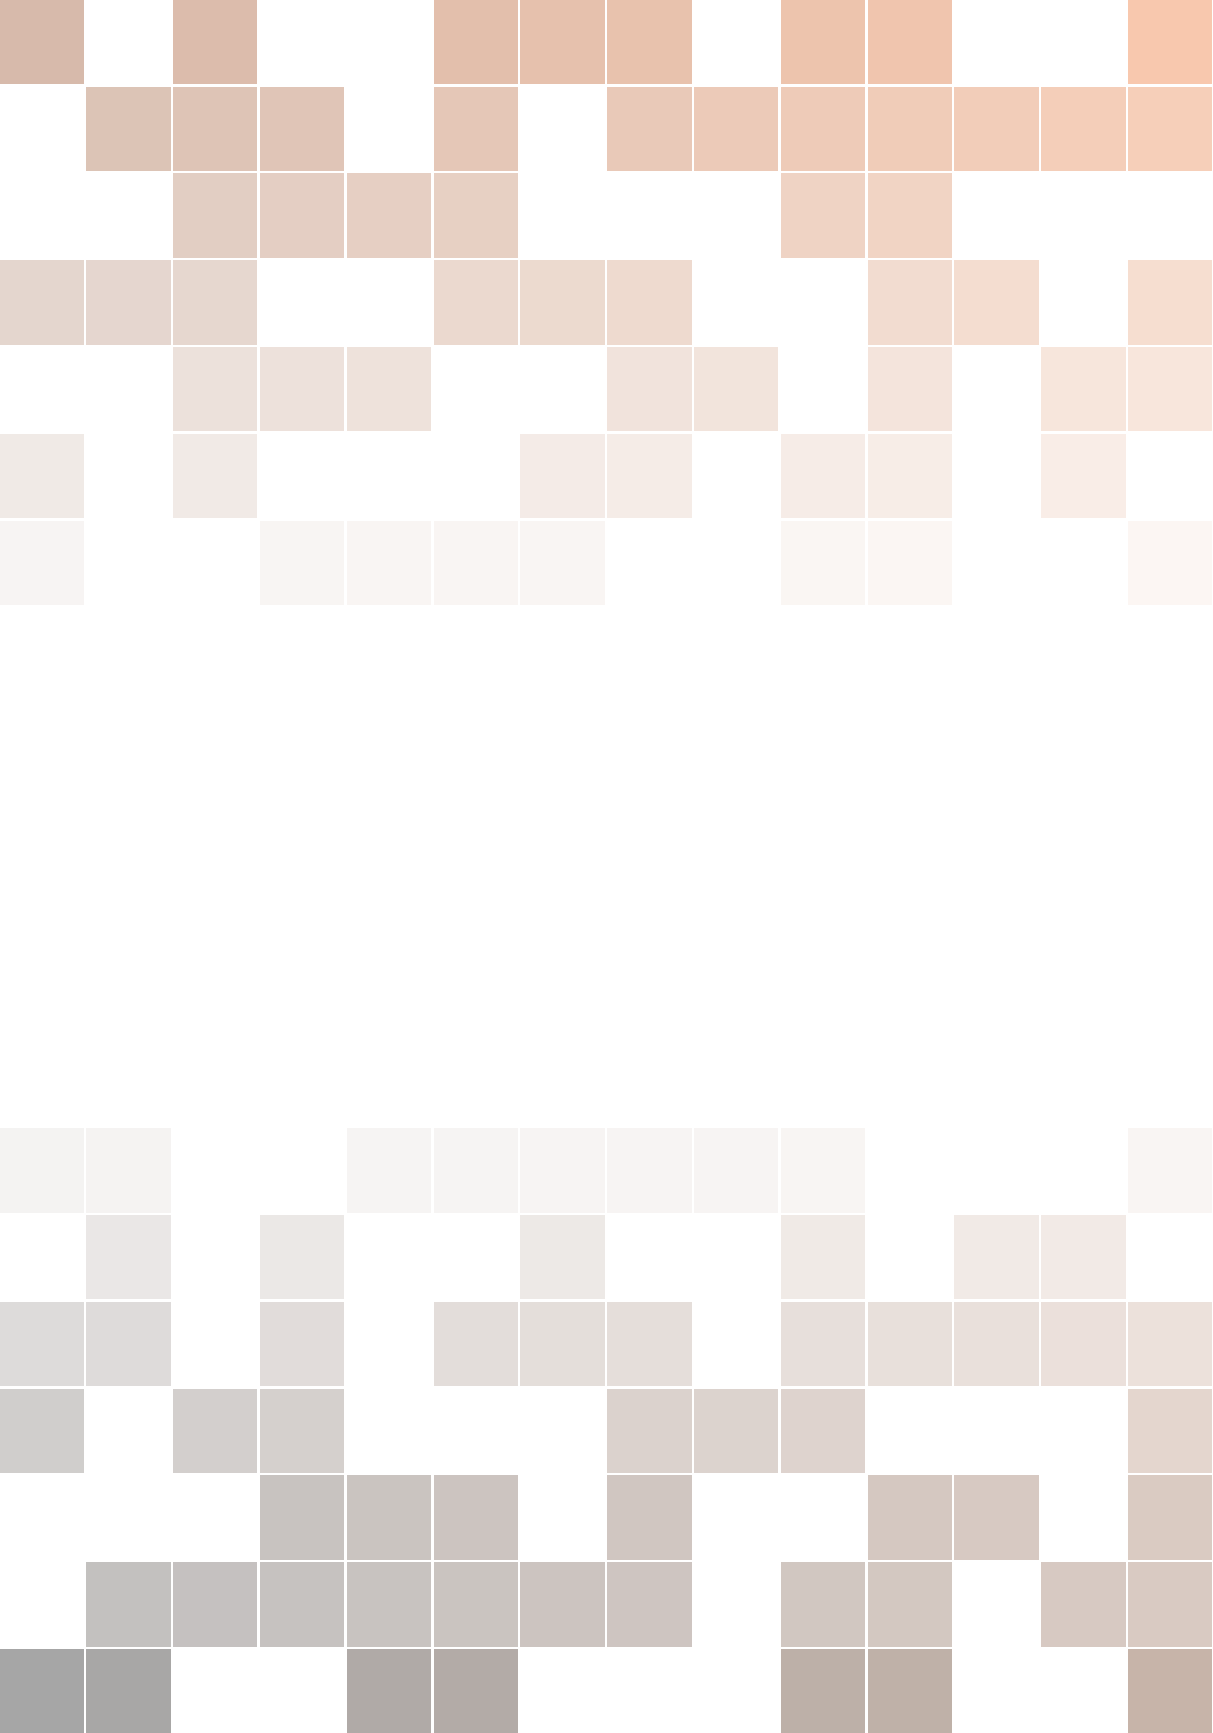
\includegraphics[width=\paperwidth]{background}};
    \draw (current page.center) node [fill=ocre!30!white,fill opacity=0.6,text opacity=1,inner sep=1cm]{\Huge\centering\bfseries\sffamily\parbox[c][][t]{\paperwidth}{\centering Introdução à Álgebra Linear\\[15pt] % Book title
            {\Large Notas de Aula \semestre/\ano}\\[20pt] % Subtitle
            {\huge José Antônio O. Freitas}\\
            {\large \today}}}; % Author name
\end{tikzpicture}
\vfill
\endgroup
%----------------------------------------------------------------------------------------
%   \COPYRIGHT PAGE
%----------------------------------------------------------------------------------------
\newpage
~\vfill
\thispagestyle{empty}

\noindent \ccbyncsa\ Este texto está licenciado sob uma \textbf{Licen\c{c}a Creative Commons Atribuição-NaoComercial-CompartilhaIgual 3.0 Brasil} \href{http://creativecommons.org/licenses/by-nc-sa/3.0/br/deed.pt\_BR}{\textit{http://creativecommons.org/licenses/by-nc-sa/3.0/br/deed.pt\_BR}}\\ % Copyright notice

%----------------------------------------------------------------------------------------
%   TABLE OF CONTENTS
%----------------------------------------------------------------------------------------
\pagestyle{empty} % Disable headers and footers for the following pages

\tableofcontents % Output the table of contents

\pagestyle{fancy} % Enable default headers and footers again

\cleardoublepage % Start the following content on a new page

%----------------------------------------------------------------------------------------
%   Capítulos
%----------------------------------------------------------------------------------------
%!TEX program = xelatex
%!TEX root = IAL.tex
%%Usar makeindex -s indexstyle.ist arquivo no terminal para gerar o {\'\i}ndice remissivo agrupado por inicial
%%Ap\'os executar pdflatex arquivo
\chapter{Matrizes}
\section{Introdução}

\subsection{Corpos}
Durante esse curso iremos trabalhar com o conceito de corpos e alguns casos específicos desse conceito.

\begin{definicao}\label{corpo}\index{Corpos}
	Um conjunto n\~ao vazio $\cp{K}$ \'e chamado de \textbf{corpo} se em $\cp{K}$ podemos definir duas opera\c{c}\~oes, denotadas por $\oplus$ (e chamada de \textbf{adi\c{c}\~ao}) e $\otimes$ (e chamada de \textbf{multiplica\c{c}\~ao}) de modo que
	\begin{align*}
		(1)\ a \oplus b \in \cp{K}\\
		(2)\ a \otimes b \in \cp{K}
	\end{align*}
	para todos $a$, $b \in \cp{K}$ e que satisfa\c{c}am as seguintes propriedades:
	\begin{enumerate}[label={\roman*})]
		\item \textbf{Comutatividade da adi\c{c}\~ao}: $a \oplus b = b \oplus a$ para todos $a$, $b \in \cp{K}$;
		\item \textbf{Associatividade da adi\c{c}\~ao}: $a \oplus (b \oplus c) = (a \oplus b) \oplus c$, para todos $a$, $b$ e $c \in \cp{K}$;
		\item \textbf{Elemento neutro da adi\c{c}\~ao}: Existe um elemento em $\cp{K}$, denotado por $0_\cp{K}$ ou simplesmente $0$ e chamado de \textbf{elemento neutro da adi\c{c}\~ao}, que satisfaz
		\[
			a \oplus 0_\cp{K} = a = 0_\cp{K} \oplus a
		\]
		para todo $a \in \cp{K}$.
		\item \textbf{Elemento oposto da adi\c{c}\~ao}: Para cada $a \in \cp{K}$, existe um elemento em $\cp{K}$, denotado por $-a$ e chamado de \textbf{oposto} de $a$ ou \textbf{inverso aditivo} de $a$ tal que
		\[
			a \oplus (-a) = 0_\cp{K} = (-a) \oplus a.
		\]
		\item \textbf{Comutatividade da multiplica\c{c}\~ao}: $a \otimes b = b \otimes a$ para todos $a$, $b \in \cp{K}$;
		\item \textbf{Associatividade da multiplica\c{c}\~ao}: $a \otimes (b \otimes c) = (a \otimes b) \otimes c$, para todos $a$, $b$ e $c \in \cp{K}$;
		\item \textbf{Elemento neutro da multiplica\c{c}\~ao}: Existe um elemento em $\cp{K}$, denotado por $1_\cp{K}$ ou simplesmente $1$ e chamado de \textbf{elemento neutro da multiplica\c{c}\~ao} ou \textbf{unidade}, que satisfaz
		\[
			a \otimes 1_\cp{K} = a = 1_\cp{K} \otimes a
		\]
		para todo $a \in \cp{K}$.
		\item \textbf{Elemento inverso da multiplica\c{c}\~ao}: Para cada $a \in \cp{K}$, $a \ne 0_{\cp{K}}$, existe um elemento em $\cp{K}$, denotado por $a^{-1}$ e chamado de \textbf{inverso multiplicativo} de $a$
		tal que
		\[
			a \otimes a^{-1} = 1_\cp{K} = a^{-1} \otimes a.
		\]
		\item \textbf{Distributividade da soma em rela\c{c}\~ao \`a multiplica\c{c}\~ao}: $(a \oplus b)\otimes c = a\otimes c \oplus b\otimes c$, para todos $a$, $b$ e $c \in \cp{K}$.
	\end{enumerate}
\end{definicao}

Para simplificar a nota\c{c}\~ao vamos escrever
\[
	a \otimes b = ab.
\]

Denotamos um corpo $\cp{K}$ pela terna $(\cp{K}, \otimes, \oplus)$. Quando n\~ao houver chance de confus\~ao em rela\c{c}\~ao \`as opera\c{c}\~oes de soma e multiplica\c{c}\~ao envolvidas no corpo $(\cp{K}, \otimes, \oplus)$, vamos simplesmente dizer que $\cp{K}$ \'e um corpo. Os elementos de um corpo $\cp{K}$ s\~ao chamados de \textbf{escalares}.

Considere $\cp{K} = \rac$ ou $\real$. Então vale sempre que:
\begin{enumerate}[label={\roman*})]
	\item $x + y = y + x$, para todos $x$, $y \in \cp{K}$;

	\item $(x + y) + z = x + (y + z)$, para todos $x$, $y$ e $z \in \cp{K}$;

	\item existe $0$ em $\cp{K}$ tal que $x + 0 = x$ para todo $x \in \cp{K}$;

	\item para cada $x \in \cp{K}$, existe $y \in \cp{K}$ tal que $x + y = 0$. Tal $y$ é escrito como $y = -x$;

	\item $xy = yx$ para todos $x$, $y \in \cp{K}$;

	\item $(xy)z = x(yz)$ para todos $x$, $y$ e $z \in \cp{K}$;

	\item existe $1 \in \cp{K}$ tal que $1x = x$ para todo $x \in \cp{K}$

	\item para todo $x \in \cp{K}$, $x \ne 0$, existe $y \in \cp{K}$ tal que $xy =1$. Tal $y$ é escrito como $y = x^{-1}$;

	\item $(x + y)z = xz + yz$ para todos $x$, $y$ e $z \in \cp{K}$.
\end{enumerate}

\subsection{Números Complexos}\index{Números Complexos}
Um outro conjunto importante com o qual iremos trabalhar é \textbf{conjunto dos números complexos}. Tal conjunto \'e definido como
\[
	\complex = \{a + bi \mid a, b \in \real, i^2 = -1\}.
\]
Dados $z = a + bi$, $w = c + di \in \complex$ definimos a soma e a multiplica\c{c}\~ao em $\complex$ por
\begin{align}
	z + w &= (a + c) + (b + d)i\label{soma_complexos}\\
	z\cdot w &= (ac - bd) + (ad + bc)i.\label{multiplicacao_complexos}
\end{align}
Al\'em disso, $a + bi = c + di$ se, e somente se, $a = c$ e $b = d$.

Dado um n\'umero complexo $z = a + bi \ne 0$, seja
\[
	w = \dfrac{a - bi}{a^2 + b^2} \ne 0.
\]
Note que
\begin{align*}
	z\cdot w = (a + bi)\cdot \dfrac{a - bi}{a^2 + b^2} = \dfrac{(a^2 + b^2) + (-ab + ba)}{a^2 + b^2} = 1
\end{align*}
assim $w$ \'e o inverso multiplicativo de $z$ em $\complex$.

O \textbf{m\'odulo}\index{Números Complexos!módulo} do n\'umero complexo $z = a + bi$ \'e definido como
\[
	|z| = \sqrt{a^2 + b^2}
\]
e o \textbf{conjugado complexo} \index{Números Complexos!conjugado complexo}de $z = a + bi$ \'e definido como
\[
	\overline{z} = a - bi.
\]

\begin{proposicao}
	Para todos $z$, $w \in \complex$ valem:
	\begin{enumerate}[label={\roman*})]
		\item $\overline{\overline{z}} = z$;
		\item $|\overline{z}| = |z|$;
		\item $z\cdot\overline{z} = |z|^2$;
		\item $\overline{z^{-1}} = \overline{z}^{-1}$;
		\item $\overline{z + w} = \overline{z} + \overline{w}$;
		\item $\overline{z \cdot w} = \overline{z} \cdot \overline{w}$;
		\item $|z \cdot w| = |z| \cdot |w|$;
	\end{enumerate}
\end{proposicao}

\begin{proposicao}
	O conjunto $\complex$ com as operações definidas em \eqref{soma_complexos} e \eqref{multiplicacao_complexos} é um corpo.
\end{proposicao}

Uma propriedade importante dos n\'umeros complexos que iremos utilizar \'e a seguinte:
\begin{teorema}
	Todo polin\^omio com coeficientes em $\complex$ possui ra{\'\i}zes complexas.
\end{teorema}

\begin{observacao}
	Um corpo satisfazendo a propriedade do teorema anterior \'e chamado de \textbf{algebricamente fechado}\index{corpo algebricamente fechado}. \'E f\'acil ver que $\rac$ e $\real$ n\~ao s\~ao corpos algebricamente fechados, isto \'e, existem polin\^omios com coeficientes em $\rac$ e em $\real$ que n\~ao possuem ra{\'\i}zes nesses corpos.
\end{observacao}
\section{Matrizes}

Durante o restante dessas notas o conjunto $\cp{K}$ representará um dos conjuntos $\rac$, $\real$ ou $\complex$.

Aqui vamos recordar algumas propriedades b\'asicas de matrizes. Para isso seja $\cp{K}$ um corpo.\index{Matriz}

Sejam $p$, $q$ dois inteiros positivos. Uma \textbf{matriz $p$ por $q$ $A$ sobre $\cp{K}$} \'e dada por $p \times q$ valores $a_{ij} \in K$, com $1 \le i \le p$, $1 \le j \le q$ agrupadas em $p$ linhas e $q$ colunas, que ser\'a representada por
\[
	A = (a_{ij})_{p\times q} = \begin{pmatrix}
		a_{11} & a_{12} & \cdots & a_{1q}\\
		a_{21} & a_{22} & \cdots & a_{2q}\\
		\vdots & & & \vdots\\
		a_{p1} & a_{p2} & \cdots & a_{pq}
	\end{pmatrix} \quad\mbox{ou}\quad
	A = [a_{ij}]_{p\times q} = \begin{bmatrix}
		a_{11} & a_{12} & \cdots & a_{1q}\\
		a_{21} & a_{22} & \cdots & a_{2q}\\
		\vdots & & & \vdots\\
		a_{p1} & a_{p2} & \cdots & a_{pq}
	\end{bmatrix}.
\]

Neste caso $A$ denota a matriz em si e o elemento de $A$ que ocorre na linha \textbf{i} e na coluna \textbf{j} é representado por $a_{ij}$.

Uma matriz $A$ com $p$ linhas e $q$ colunas é dita possuir \textbf{ordem}\index{Matriz!ordem}, ou \textbf{tamanho}, $p\times q$.

\begin{exemplo}
	A matriz $A$ dada a seguir:
	\[
		A = \begin{bmatrix}
			-1 & 0 & 1/2 & 1\\
			2 & \sqrt{2} & 3 & 3\\
			0 & 0 & \pi & 0
		\end{bmatrix}
	\]
	é uma matriz de ordem $3 \times 4$.

	Nessa matriz
	\begin{itemize}
		\item O elemento $a_{12}$ de $A$ é $a_{12} = 0$;

		\item O elemento $a_{24}$ de $A$ é $a_{24} = 3$;

		\item O elemento $a_{33}$ de $A$ é $a_{12} = \pi$.
	\end{itemize}
\end{exemplo}

\begin{definicao}
	Seja
	\[
		A = (a_{ij})_{p\times q} = \begin{bmatrix}
			a_{11} & a_{12} & \cdots & a_{1q}\\
			a_{21} & a_{22} & \cdots & a_{2q}\\
			\vdots & & & \vdots\\
			a_{p1} & a_{p2} & \cdots & a_{pq}
		\end{bmatrix}
	\]
	uma matriz de ordem $p\times q$ com entradas num corpo $\cp{K}$.

	\begin{enumerate}
		\item Se $p \ne q$, $A$ é chamada de uma \textbf{matriz retangular}.\index{Matriz!retangular}

		\item Se $A$ tem ordem $p \times 1$, isto é, se $A$ possui $p$ linhas e somente \textbf{uma coluna}, dizemos que $A$ é uma \textbf{matriz coluna}\index{Matriz!coluna}. Nesse caso $A$ tem a forma:
		\[
			A = \begin{pmatrix}a_{11}\\a_{21}\\\vdots\\a_{p - 11}\\a_{p1}\end{pmatrix}.
		\]
		\item Se $A$ tem ordem $1 \times q$, isto é, se $A$ possui somente \textbf{uma linhas} e $q$ colunas, dizemos que $A$ é uma \textbf{matriz linha}\index{Matriz!linha}. Nesse caso $A$ tem a forma:
		\[
			A = \begin{pmatrix}a_{11} & a_{12} & \cdots & a_{1n-1} & a_{1q}\end{pmatrix}.
		\]
		\item Se $p = q$, então $A$ é chamada de \textbf{matriz quadrada} e a ordem de $A$ é $p \times p$ ou simplesmente $p$. Neste caso $A$ tem a forma:
		\[
			A = (a_{ij})_{p\times p} = \begin{pmatrix}
				a_{11} & a_{12} & \cdots & a_{1p}\\
				a_{21} & a_{22} & \cdots & a_{2p}\\
				\vdots & & & \vdots\\
				a_{p1} & a_{p2} & \cdots & a_{pp}
			\end{pmatrix}.
		\]
	\end{enumerate}
\end{definicao}

\begin{exemplo}
	\begin{enumerate}
		\item A matrix
		\[
			A = \begin{pmatrix}
				-1 & 2 & -3/7 & 9
			\end{pmatrix}
		\]
		é uma matriz-linha de ordem $1 \times 4$.
		\item A matrix
		\[
			B = \begin{bmatrix}
				-1 \\ \phantom{-}2 \\ -3/7 \\ \phantom{-}9
			\end{bmatrix}
		\]
		é uma matriz-coluna de ordem $4 \times 1$.
		\item A matrix
		\[
			C = \begin{pmatrix}
				-1 & 2 & -3/7 & 9\\
				-1 & 2 & -3/7 & 9\\
				-1 & 2 & -3/7 & 9\\
				-1 & 2 & -3/7 & 9\\
			\end{pmatrix}
		\]
		é uma matriz quadrada de ordem $r \times 4$.
		\item A matrix
		\[
			D = \begin{bmatrix}
				-1 & 2 & -3/7 & 9\\
				-9 & 3/7 & -2 & 1
			\end{bmatrix}
		\]
		é uma matriz retangular de ordem $2 \times 4$.
	\end{enumerate}
\end{exemplo}

Seja
\[
	A = \begin{bmatrix}
		a_{11} & a_{21} & \cdots & a_{1q}\\
		a_{21} & a_{22} & \cdots & a_{2q}\\
		\vdots & \vdots & & \vdots\\
		a_{p1} & a_{p2} & \cdots & a_{pq}
	\end{bmatrix}
\]
uma matriz de ordem $p\times q$. Denotamos a $i$-ésima linha, $1 \le i \le p$, de $A$ por
\[
	A_i = \begin{bmatrix}a_{i1} & a_{i2} & \cdots & a_{iq}\end{bmatrix}.
\]
Denotamos a $j$-ésima coluna, $1 \le j \le q$, de $A$ por
\[
	A^j = \begin{bmatrix}a_{1j} \\ a_{2j} \\ \vdots \\ a_{pj}\end{bmatrix}.
\]

\begin{exemplo}
	Considere a matriz
	\[
		A = \begin{pmatrix}
			\phantom{-} 1 & 2 + i & 2 - 3i\\
			-2 & 0 & \pi - i\sqrt{2}
		\end{pmatrix}
	\].
	Neste caso as linhas de $A$ são:
	\begin{align*}
		A_1 &= \begin{pmatrix}\phantom{-} 1 & 2 + i & 2 - 3i\end{pmatrix}\\
		A_2 &= \begin{pmatrix}-2 & 0 & \pi - i\sqrt{2}\end{pmatrix}.
	\end{align*}
	As colunas de $A$ são:
	\begin{align*}
		A^1 &= \begin{pmatrix}
			\phantom{-} 1\\-2
			\end{pmatrix}\\
		A^2 &= \begin{pmatrix}
			2 + i\\0
			\end{pmatrix}\\
		A^3 &= \begin{pmatrix}
			2 - 3i\\\pi - i\sqrt{2}
			\end{pmatrix}\\
	\end{align*}
\end{exemplo}

Dada uma matriz quadrada de ordem $p$
\[
	A = \begin{pmatrix}
		a_{11} & a_{21} & \cdots & a_{1p}\\
		a_{21} & a_{22} & \cdots & a_{2p}\\
		\vdots & \vdots & & \vdots\\
		a_{p1} & a_{p2} & \cdots & a_{pp}
	\end{pmatrix}
\]
os elementos $a_{ij}$ de $A$ com $i = j$ formam a \textbf{diagonal princial} de $A$:\index{Matriz!diagonal principal}
\[
	\begin{pmatrix}
		\tikzmarknode{top}{a_{11}} & a_{12} & a_{13} & \cdots  & a_{1p}\\
		a_{21} & a_{22} \phantom{-} & a_{23} & \cdots  & a_{2n}\\
		a_{31} & a_{32}\phantom{-} & a_{33} \phantom{-1} & \cdots  & a_{3p}\\
		\vdots  & \vdots   & \vdots  & \vdots  & \vdots\\
		a_{p1} & a_{p2} & a_{p3} & \cdots  & \tikzmarknode{bottom}{a_{pp}}\\
	\end{pmatrix}
\]

\begin{tikzpicture}[overlay, remember picture]
	\draw[red, opacity=.5, line width=5mm, line cap=round] (top.north west) -- (bottom.south east);
\end{tikzpicture}

Os elementos $a_{ij}$ com $i + j = p + 1$ formam a \textbf{diagonal secundária} de $A$:\index{Matriz!diagonal secundária}
\[
	\begin{pmatrix}
		a_{11} & a_{12} & a_{13} & \cdots  & a_{1p-1} & \tikzmarknode{top_right}{a_{1p}}\\
		a_{21} & a_{22} & a_{23} & \cdots  & a_{2p-1} & a_{2p}\\
		a_{31} & a_{32} & a_{33} & \cdots  & \phantom{-}a_{3p-1} & a_{3p}\\
		\vdots  & \vdots   & \vdots  & \vdots  & \vdots\\
		\tikzmarknode{bottom_left}{a_{p1}} & \phantom{-} a_{p2} & a_{p3} & \cdots  & a_{pp-1} & {a_{pp}}\\
	\end{pmatrix}
\]

\begin{tikzpicture}[overlay, remember picture]
	\draw[blue, opacity=.5, line width=5mm, line cap=round] (top_right.north east) -- (bottom_left.south west);
\end{tikzpicture}

\begin{definicao}
    Seja
    \[
        A = \begin{bmatrix}
                a_{11} & \cdots & a_{1n}\\
                a_{21} & \cdots & a_{2n}\\
                \vdots & \ddots & \vdots\\
                a_{n1} & \cdots & a_{nn}
            \end{bmatrix}
    \]
    uma matriz quadrada de ordem $p$. Dizemos que:
    \begin{enumerate}
        \item $A$ é uma \textbf{matriz diagonal}\index{Matriz!diagonal} se $a_{ij} = 0$ para todo $i \ne j$. Assim $A$ é uma matriz da forma
            \[
                A = \begin{bmatrix}
                    a_{11} & 0 & \cdots & 0\\
                    0 & a_{22} & \cdots & 0\\
                    \vdots & \vdots & \ddots & \vdots\\
                    0 & \cdots & 0 & a_{nn}
                \end{bmatrix}.
            \]

        \item $A$ é uma \textbf{matriz unidade} ou \textbf{matriz identidade} ou ainda que $A$ é uma \textbf{matriz unitária} de
            \textbf{ordem} $n$ se $A$ é uma matriz diagonal e $a_{ii} = 1$ para $1 \le i \le n$. Neste caso denotamos tal matriz por $I_n$ e
        \[
            I_n = \begin{bmatrix}
                1 & 0 & \cdots & 0\\
                0 & 1 & \cdots & 0\\
                \vdots & \vdots & \ddots & \vdots\\
                0 & \cdots & 0 & 1
            \end{bmatrix}.
        \]
    \item $A$ é uma \textbf{matriz triangular inferior}\index{Matriz!triangular inferior} se $a_{ij} = 0$ para $i < j$. Assim $A$ será uma matriz da forma
    \[
        A = \begin{bmatrix}
                a_{11} & 0 & 0 & \cdots & 0\\
                a_{21} & a_{22} & 0 & \cdots & 0\\
                \vdots & \vdots & \ddots & & \vdots\\
                a_{n1} & a_{n2} & \cdots & \cdots &  a_{nn}
        \end{bmatrix}.
    \]
    \item $A$ é uma \textbf{matriz triangular superior}\index{Matriz!triangular superior} se $a_{ij} = 0$ para $i > j$. Assim $A$ será uma matriz da forma
    \[
        A = \begin{bmatrix}
                a_{11} & a_{12} & a_{13} & \cdots & a_{1n}\\
                0 & a_{22} & a_{23} & \cdots & a_{2n}\\
                \vdots & \vdots & \ddots & & \vdots\\
                0 & 0 & \cdots & 0 &  a_{nn}
        \end{bmatrix}.
    \]
    \end{enumerate}
\end{definicao}

\begin{exemplos}
    \begin{enumerate}
        \item A matriz
            \[
                A = \begin{pmatrix}
                    2 & -1/2 & 3 & \phantom{-}4\\
                    0 & \phantom{-}0 & 1 & -2\\
                    0 & \phantom{-}0 & 4 & \phantom{-}\sqrt{2}\\
                    0 & \phantom{-}0 & 0 & \phantom{-}1
                \end{pmatrix}
            \]
        é uma matriz triangular superior de ordem 4.
        \item A matriz
            \[
                B = \begin{pmatrix}
                    2 & \phantom{-}0 & \phantom{-}0 & 0\\
                    1 & -3i & \phantom{-}0 & 0\\
                    i & -1 & \phantom{-}4 & 0\\
                    7 & \phantom{-}3 & -2 & 5
                \end{pmatrix}
            \]
        é uma matriz triangular inferior de ordem 4.
        \item A matriz
            \[
                C = \begin{pmatrix}
                    1 & 0 & 0\\
                    0 & 1 & 0\\
                    0 & 0 & 1
                \end{pmatrix}
            \]
        é a matriz identidade de ordem 3.
        \item A matriz
            \[
                D = \begin{pmatrix}
                    2 & 0\\
                    0 & 3
                \end{pmatrix}
            \]
        é uma matriz diagonal de ordem 2.
    \end{enumerate}
\end{exemplos}

\begin{definicao}
    Seja $A$ uma matriz de ordem $p\times q$. Dizemos que $A$ é uma \textbf{matriz nula}\index{Matriz!nula} se $a_{ij} = 0$ para todo $1 \le i \le p$ e todo $1 \le j \le p$. Neste caso escrevemos $A_{p\times q} = 0_{p\times q}$.
\end{definicao}

\begin{exemplo}
    \begin{enumerate}
        \item $0_2 = \begin{pmatrix} 0 & 0\\0 & 0\end{pmatrix}$ é a matrz nula de ordem 2.

        \item $0_{2 \times 3} = \begin{pmatrix}0 & 0 & 0\\0 & 0 & 0\end{pmatrix}$ é a matriz nula de ordem $2 \times 3$.
    \end{enumerate}
\end{exemplo}

\begin{notacao}
	Denotaremos o conjunto de todas as matrizes $p\times q$ sobre $\cp{K}$ por $M_{p\times q}(\cp{K})$, onde $\cp{K} = \rac$, $\real$ ou $\complex$. Assim
	\[
		M_{p\times q}(\cp{K}) = \left\{\begin{bmatrix}
			a_{11} & a_{12} & \cdots & a_{1p}\\
			a_{21} & a_{22} & \cdots & a_{2p}\\
			\vdots & & & \vdots\\
			a_{p1} & a_{p2} & \cdots & a_{pq}\end{bmatrix} \mid a_{ij} \in \cp{K},\ 1 \le i \le p,\ 1 \le j \le q
		\right\}
	\]
\end{notacao}

Por exemplo,
\[
	M_{3\times 2}(\real) = \left\{\begin{pmatrix}a_{11} & a_{12}\\a_{21} & a_{22}\\ a_{31} & a_{32}\end{pmatrix} \mid a_{ij} \in \real,\ 1 \le i \le 3,\ 1 \le j \le 2\right\}.
\]


No caso em que $p = q = n$ iremos escrever simplesmente
\[
	M_{n\times n}(\cp{K}) = M_n(\cp{K}).
\]

Nesse conjunto podemos definir as seguintes opera\c{c}\~oes:
\begin{enumerate}
    \item \textit{Igualdade de matrizes:}\index{Matriz!igualdade} Sejam $A = (a_{ij})$ e $B = (b_{ij})$ matrizes em $M_{p\times q}(\cp{K})$. Então dizemos que $A$
        e $B$ são \textbf{iguais} quando $a_{ij} = b_{ij}$ para todo $1 \le i \le p$ e todo $1 \le j \le q$.

    \item \textit{Soma de matrizes:}\index{Matrizes!soma} Se $A = (a_{ij})$, $B = (b_{ij}) \in M_{p\times q}(\cp{K})$, ent\~ao a
        \textbf{soma} $A + B$ \'e a matriz $C = (c_{ij}) \in M_{p\times q}(\cp{K})$, tal que, para cada par $(i,j)$ temos $c_{ij} = a_{ij} + b_{ij}$, ou seja,
	\begin{align*}
		C = A + B &= \begin{pmatrix}
		a_{11} & a_{12} & \cdots & a_{1q}\\
		a_{21} & a_{22} & \cdots & a_{2q}\\
		\vdots & & & \vdots\\
		a_{p1} & a_{p2} & \cdots & a_{pq}
	\end{pmatrix} + \begin{pmatrix}
		b_{11} & b_{12} & \cdots & b_{1q}\\
		b_{21} & b_{22} & \cdots & b_{2q}\\
		\vdots & & & \vdots\\
		b_{p1} & b_{p2} & \cdots & b_{pq}
	\end{pmatrix}\\ &= \begin{pmatrix}
		a_{11} + b_{11} & a_{12} + b_{12} & \cdots & a_{1q} + b_{1q}\\
		a_{21} + b_{21} & a_{22} + b_{22}& \cdots & a_{2q} + b_{1q}\\
		\vdots & & & \vdots\\
		a_{p1} + b_{p1} & a_{p2} + b_{p2}& \cdots & a_{pq} + b_{pq}
	\end{pmatrix}
	\end{align*}

    \item \textit{Diferença de matrizes:}\index{Matrizes!diferença} Se $A = (a_{ij})$, $B = (b_{ij}) \in M_{p\times q}(\cp{K})$, ent\~ao a
        \textbf{diferença} $A - B$ \'e a matriz $C = (c_{ij}) \in M_{p\times q}(\cp{K})$, tal que, para cada par $(i,j)$ temos $c_{ij} =
        a_{ij} - b_{ij}$, ou seja,
	\begin{align*}
		C = A - B &= \begin{pmatrix}
		a_{11} & a_{12} & \cdots & a_{1q}\\
		a_{21} & a_{22} & \cdots & a_{2q}\\
		\vdots & & & \vdots\\
		a_{p1} & a_{p2} & \cdots & a_{pq}
	\end{pmatrix} - \begin{pmatrix}
		b_{11} & b_{12} & \cdots & b_{1n}\\
		b_{21} & b_{22} & \cdots & b_{2n}\\
		\vdots & & & \vdots\\
		b_{p1} & b_{p2} & \cdots & b_{pq}
	\end{pmatrix}\\ &= \begin{pmatrix}
		a_{11} - b_{11} & a_{12} - b_{12} & \cdots & a_{1q} - b_{1q}\\
		a_{21} - b_{21} & a_{22} - b_{22}& \cdots & a_{2q} - b_{1q}\\
		\vdots & & & \vdots\\
		a_{p1} - b_{p1} & a_{p2} - b_{p2}& \cdots & a_{pq} - b_{pq}
	\end{pmatrix}
	\end{align*}
\end{enumerate}

\begin{exemplo}
    Sejam
    \[
        A = \begin{pmatrix}1 & \phantom{-}2 & 1/3\\0 & -3 & 2/3\end{pmatrix}\\
        \mbox{e}\\
        B = \begin{pmatrix}2 & -3 & 3\\0 & \phantom{-}2 & 2/3\end{pmatrix}.
    \]
    Então
    \begin{align*}
        A + B &= \begin{pmatrix} 3 & -1 & 10/3\\0 & -1 & 4/3\end{pmatrix}\\
        A - B &= \begin{pmatrix} -1 & \phantom{-}5 & -8/3\\ \phantom{-}0 & -5 & \phantom{-}0\end{pmatrix}
    \end{align*}
\end{exemplo}

\begin{proposicao}
	Dadas matrizes $A$, $B$ e $C \in M_{p\times q}(\cp{K})$ vale:
	\begin{enumerate}[label={\roman*})]
		\item $(A + B) + C = A + (B + C)$
		\item $A + B = B + A$
        \item $0_{p\times q} + A = A = A + 0_{p\times q}$
        \item $A - A = 0_{p\times q}$.
	\end{enumerate}
\end{proposicao}

\begin{observacao}
    Os elementos de um corpo $\cp{K}$ serão chamados de \textbf{escalares}.
\end{observacao}

\begin{definicao}
    Seja $A = (a_{ij}) \in M_{p\times q}(\cp{K})$ e $\lambda \in \cp{K}$ definimos o \textbf{produto escalar}\index{Matriz!produto escalar} de $\lambda$ por $A$ como sendo a matriz $B = (b_{ij}) \in M_{p\times q}(\cp{K})$ onde para cada para $(i,j)$ temos $b_{ij} = \lambda a_{ij}$:
	\begin{align*}
		\lambda A = \lambda \begin{pmatrix}
		a_{11} & a_{12} & \cdots & a_{1q}\\
		a_{21} & a_{22} & \cdots & a_{2q}\\
		\vdots & & & \vdots\\
		a_{p1} & a_{p2} & \cdots & a_{pq}
	\end{pmatrix} = \begin{pmatrix}
		\lambda a_{11} & \lambda a_{12} & \cdots & \lambda a_{1q}\\
		\lambda a_{21} & \lambda a_{22} & \cdots & \lambda a_{2q}\\
		\vdots & & & \vdots\\
		\lambda a_{p1} & \lambda a_{p2} & \cdots & \lambda a_{pq}
	\end{pmatrix}.
	\end{align*}
\end{definicao}
\begin{exemplo}
    Seja $\lambda = 2 \in \real$ e
    \[
        A = \begin{bmatrix}
            1 & \sqrt{2} & \phantom{-}1/2\\
            \pi & 2 & -1
        \end{bmatrix}.
    \]
    Então
    \begin{align*}
        \lambda A = 2A = \begin{bmatrix}
            2 & 2\sqrt{2} & \phantom{-}1\\
            2\pi & 4 & -2
        \end{bmatrix}
    \end{align*}
\end{exemplo}

\begin{proposicao}
    Sejam $A \in M_{p\times q}(\cp{K})$ e  $B \in M_{p\times q}(\cp{K})$ e $\alpha$, $\lambda \in \cp{K}$, ent\~ao:
	\begin{enumerate}[label={\roman*})]
		\item $(\alpha\lambda) A = \alpha(\lambda A) = \lambda(\alpha A)$
		\item $(\alpha + \lambda)A = \alpha A + \lambda A$
        \item $\alpha(A + B) = \alpha A + \alpha B$
        \item $1A = A$ e $(-1)A = -A$
        \item  $0A = 0_{p\times q}$
	\end{enumerate}
\end{proposicao}

\begin{observacao}
    Dadas matrizes $A_1$, $A_2$, \dots, $A_l \in M_{p\times q}(\cp{K})$ e escalares $\lambda_1$, $\lambda_2$, \dots, $\lambda_l \in \cp{K}$
    podemos definir a soma
    \[
        \lambda_1 A_1 + \lambda_2 A_2 + \cdots + \lambda_l A_l
    \]
    que é chamada de \textbf{combinação linear} de $A_1$, $A_2$, \dots, $A_l$ com os escalares $\lambda_1$, $\lambda_2$, \dots, $\lambda_l$. Por exemplo, tomando
    \[
        A_1 = \begin{pmatrix}1\\2\\3\end{pmatrix}, A_2 = \begin{pmatrix}-1\\\phantom{-}0\\-3\end{pmatrix}, A_3 = \begin{pmatrix}-1\\\phantom{-}2\\\phantom{-}3\end{pmatrix}
    \]
    e $\lambda_1 = 2$, $\lambda_2 = -1$ e $\lambda_3 = 3$ obtemos
    \begin{align*}
        \lambda_1 A_1 + \lambda_2 A_2 + \lambda_3 A_3 &= 2A_1 + (-1)A_2 + 3A_3\\ &= 2\begin{pmatrix}1\\2\\3\end{pmatrix} + (-1)
        \begin{pmatrix}-1\\\phantom{-}0\\-3\end{pmatrix} +3\begin{pmatrix}-1\\\phantom{-}2\\\phantom{-}3\end{pmatrix}\\ &= \begin{pmatrix}2 + 1 - 3\\4 + 0 + 6\\6 + 3 +
        9\end{pmatrix} = \begin{pmatrix}-2\\\phantom{-}10\\\phantom{-}18\end{pmatrix}
    \end{align*}
\end{observacao}

\begin{definicao}
    Seja $A = (a_{ij})_{p\times q}$ uma matriz de ordem $p\times q$. A \textbf{matriz transposta}\index{Matriz!transposta} é a matriz
    denotada por $A^T = (b_{ij})$ com $b_{ij} = a_{ji}$ para todo $1 \le i \le p$, $1 \le j \le q$, de ordem $q \times p$.
\end{definicao}

\begin{exemplos}
    \begin{enumerate}
        \item Seja $A$ uma matriz qualquer, de ordem $2 \times 3$.
            Assim escrevendo
            \[
                A = \begin{pmatrix}
                        a_{11} & a_{12} & a_{13}\\
                        a_{21} & a_{22} & a_{23}
                    \end{pmatrix}
            \]
            então a \textbf{matriz transposta} de $A$ será
            \[
                A^T = \begin{pmatrix}
                        a_{11} & a_{21}\\
                        a_{12} & a_{22}\\
                        a_{13} & a_{23}
                    \end{pmatrix}
            \]
            que é uma matriz de ordem $3 \times 2$.

        \item Seja $B$ uma matriz qualquer, de ordem $3 \times 3$.
            Assim escrevendo
            \[
                B = \begin{pmatrix}
                        b_{11} & b_{12} & b_{13}\\
                        b_{21} & b_{22} & b_{23}\\
                        b_{31} & b_{32} & b_{33}
                    \end{pmatrix}
            \]
            então a \textbf{matriz transposta} de $B$ será
            \[
                B^T = \begin{pmatrix}
                        b_{11} & b_{21} & b_{31}\\
                        b_{12} & b_{22} & b_{32}\\
                        b_{13} & b_{23} & b_{33}
                    \end{pmatrix}
            \]
            que é uma matriz de ordem $3 \times 3$.

        \item Se $A = \begin{pmatrix}1 \\ 3\\ 0\end{pmatrix}$ é uma matriz $3 \times 1$, então
            \[
                A^T = \begin{pmatrix}1 & 3 & 0\end{pmatrix}
            \]
            é uma matriz $1 \times 3$.

        \item Seja $B = \begin{pmatrix}1 & -2\\3 & \sqrt{3}\end{pmatrix}$, então
            \[
                B^T = \begin{pmatrix}
                    \phantom{-}1 & 3\\
                    -2 & \sqrt{3}
                \end{pmatrix}
            \]
    \end{enumerate}
\end{exemplos}


\begin{proposicao}
    Sejam $A$, $B \in M_{p\times q}(\cp{K})$ e $\alpha \in \cp{K}$. Então:
    \begin{enumerate}
        \item $(A^T)^T = A$

        \item $(\alpha A)^T = \alpha(A^T)$

        \item $(A + B)^T = A^T + B^T$

        \item $(A - B)^T = A^T - B^T$
    \end{enumerate}
\end{proposicao}

\begin{definicao}
    Seja $A \in M_n(\cp{K})$. Definimos o \textbf{traço}\index{Matriz!traço} da matriz $A$ como o escalar dado por
    \[
        \tr{A} = a_{11} + a_{22} + \cdots + a_{nn},
    \]
    isto é, o traço de $A$ é a \textbf{soma} dos elementos da \textbf{diagonal princial} de $A$.
\end{definicao}

\begin{proposicao}
    Dadas matrizes $A$, $B \in M_n(\cp{K})$ e $\lambda \in \cp{K}$, então
    \begin{enumerate}
        \item $\tr{A^T} = \tr{A}$

        \item $\tr{\lambda A} = \lambda\tr{A}$

        \item $\tr{A + B} = \tr{A} + \tr{B}$
    \end{enumerate}
\end{proposicao}

\begin{definicao}
    Seja $A = (a_{ij})\in M_n(\cp{K})$.
    \begin{enumerate}
        \item Dizemos que $A$ é uma \textbf{matriz simétrica}\index{Matriz!simétrica} se $A = A^T$, ou seja, se $a_{ij} = a_{ji}$ para todos $i, j$.
        \item Dizemos que $A$ é uma \textbf{matriz anti-simétrica}\index{Matriz!anti-simétrica} se $A^T = -A$, ou seja, se $a_{ji} =
            -a_{ij}$ para todos $i, j$. Neste caso devemos ter $a_{ii} = 0$ para $1 \le i \le n$.
    \end{enumerate}
\end{definicao}

\begin{exemplos}
    \begin{enumerate}
        \item A matriz
            \[
                A = \begin{pmatrix}
                    1 & 2\\
                    2 & 1
                \end{pmatrix}
            \]
            é uma matriz simétrica pois
            \[
                A^T = \begin{pmatrix}
                    1 & 2\\
                    2 & 1
                \end{pmatrix} = A.
            \]

        \item A matriz
            \[
                B = \begin{pmatrix}
                    \phantom{-}1 & \phantom{-}0 & -2\\
                    \phantom{-}0 & -2 & \phantom{-}3\\
                    -2 & \phantom{-}3 & \phantom{-}4
                \end{pmatrix}
            \]
            é uma matriz simétrica pois
            \[
                B^T = \begin{pmatrix}
                    \phantom{-}1 & \phantom{-}0 & -2\\
                    \phantom{-}0 & -2 & \phantom{-}3\\
                    -2 & \phantom{-}3 & \phantom{-}4
                \end{pmatrix} = B
            \]

        \item A matriz
            \[
                C = \begin{pmatrix}
                   \phantom{-} 0 & \phantom{-}1 & -2\\
                    -1 & \phantom{-}0 & \phantom{-}3\\
                    \phantom{-}2 & -3 & \phantom{-}0
                \end{pmatrix}
            \]
            é uma matriz anti-simétrica pois
             \[
                C^T = \begin{pmatrix}
                    \phantom{-}0 & -1 & \phantom{-}2\\
                    \phantom{-}1 & \phantom{-}0 & -3\\
                    -2 & \phantom{-}3 & \phantom{-}0
                \end{pmatrix} = -C
            \]

        \item A matriz
            \[
                D = \begin{pmatrix}
                    0 & -2\\
                    2 & \phantom{-}0
                \end{pmatrix}
            \]
            é uma matriz anti-simétrica pois
            \[
                D^T = \begin{pmatrix}
                    \phantom{-}0 & 2\\
                    -2 & 0
                \end{pmatrix} = -D.
            \]

        \item A matriz
            \[
                E = \begin{pmatrix}
                    1 & 0 & -1 & 5\\
                    2 & 0 & \phantom{-}1 & 3\\
                    4 & 0 & -1 & 5\\
                    1 & 0 & -1 & 5
                \end{pmatrix}
            \]
            não é nem uma matriz simétrica e nem uma matriz anti-simétrica pois
            \[
                E^T = \begin{pmatrix}
                    \phantom{-}1 & \phantom{-}2 & \phantom{-}4 & \phantom{-}1\\
                    \phantom{-}0 & \phantom{-}0 & \phantom{-}0 & \phantom{-}0\\
                    -1 & \phantom{-}1 & -1 & -1\\
                    \phantom{-}5 & \phantom{-}3 & \phantom{-}5 & \phantom{-}5
                \end{pmatrix}
            \]
            e nesse caso $E \ne E^T$ e $E^T  \ne -E$.
    \end{enumerate}
\end{exemplos}


\begin{definicao}
	Sejam $A = (a_{ij}) \in M_{p\times q}(\cp{K})$ e $B = (b_{ij}) \in M_{q\times r}(\cp{K})$, definimos o \textbf{produto de $A$ por
    $B$}\index{Matrizes!produto de} como sendo a matriz $C = (c_{ij}) \in M_{p\times r}(\cp{K})$ tal que
	\[
        c_{ij} = a_{i1}b_{1j} + a_{i2}b_{2j} + \cdots + a_{iq}b_{qj},
	\]
	para $i = 1$, \dots, $p$ e $j = 1$, \dots, $r$. Isto \'e,
	\begin{align*}
		A\cdot B &= \begin{pmatrix}
		a_{11} & a_{12} & \cdots & a_{1q}\\
		a_{21} & a_{22} & \cdots & a_{2q}\\
		\vdots & & & \vdots\\
		a_{p1} & a_{p2} & \cdots & a_{pq}
	\end{pmatrix}\cdot \begin{pmatrix}
		b_{11} & b_{12} & \cdots & b_{1r}\\
		b_{21} & b_{22} & \cdots & b_{2r}\\
		\vdots & & & \vdots\\
		b_{q1} & b_{q2} & \cdots & b_{qr}
        \end{pmatrix} \\ &= \begin{pmatrix}
        a_{11}b_{11} + a_{12}b_{21} + \cdots + a_{1q}b_{q1} & a_{11}b_{12} + a_{12}b_{22} + \cdots + a_{1q}b_{q2} & \dots & a_{11}b_{1r} +
        a_{12}b_{2r} + \\ & & & \cdots + a_{1r}b_{qr}\\
        a_{21}b_{11} + a_{22}b_{21} + \cdots + a_{2q}b_{q1} & a_{21}b_{12} + a_{22}b_{22} + \cdots + a_{2q}b_{q2} & \dots & a_{21}b_{1r} +
        a_{12}b_{2r} +\\ & & & \cdots + a_{1q}b_{qr}\\
        \vdots & \vdots & \cdots & \vdots\\
         a_{p1}b_{11} + a_{p2}b_{21} + \cdots + a_{pq}b_{n1} & a_{p1}b_{12} + a_{p2}b_{22} + \cdots + a_{pq}b_{q2} & \dots & a_{p1}b_{1r} +
         a_{p2}b_{2r} + \\ & & & \cdots + a_{pq}b_{qr}\\
        \end{pmatrix}
	\end{align*}
\end{definicao}
\begin{exemplos}
    \begin{enumerate}
        \item Considere as matrizes
            \[
                A = \begin{pmatrix}
                    1 & \phantom{-}2 & -3\\
                    0 & -1 & -2
                \end{pmatrix},
                B = \begin{pmatrix}
                    \phantom{-}3 & 1\\
                    -2 & 2\\
                    \phantom{-}4 & 0
                \end{pmatrix}.
            \]
            Como $A$ é uma matriz $2 \times 3$ e $B$ é uma matriz $3 \times 2$, então o produto $AB$ está definido e o resultado será uma
            matriz $C$ de ordem $2 \times 2$.
            \begin{align*}
                C &= AB = \begin{pmatrix}
                    1 & \phantom{-}2 & -3\\
                    0 & -1 & -2
                \end{pmatrix}
                \begin{pmatrix}
                    \phantom{-}3 & 1\\
                    -2 & 2\\
                    \phantom{-}4 & 0
                \end{pmatrix} \\ &=
                \begin{pmatrix}
                    1\cdot 3 + 2\cdot(-2) + (-3)\cdot4 & 1\cdot 1 + 2\cdot 2 + (-3)\cdot 0\\
                    0\cdot 3 + (-1)\cdot(-2) + (-2) \cdot 4 & 0\cdot 1 + (-1)\cdot 2 + (-2)\cdot 0
                    \end{pmatrix}\\ &= \begin{pmatrix}
                        -13 & 5\\
                        -5 & -2
                    \end{pmatrix}
                \end{align*}
        \item Considere as matrizes
            \[
                A = \begin{pmatrix}
                    -2 & \phantom{-}2\\
                    \phantom{-}2 & -1\\
                    \phantom{-}1/2 & \phantom{-}3
                \end{pmatrix},
                B = \begin{pmatrix}
                    \phantom{-}3 & -1 & \phantom{-}1 &2\\
                    -2 & \phantom{-}1 & -3 & 2
                \end{pmatrix}.
            \]
            Como $A$ é uma matriz $3 \times 2$ e $B$ é uma matriz $2 \times 4$, então o produto $AB$ está definido e o resultado será uma
            matriz $C$ de ordem $3 \times 4$.
            \begin{align*}
                C &= AB = \begin{pmatrix}
                    -2 & \phantom{-}2\\
                    \phantom{-}2 & -1\\
                    \phantom{-}1/2 & \phantom{-}3
                \end{pmatrix}
                \begin{pmatrix}
                    \phantom{-}3 & -1 & \phantom{-}1 & 2\\
                    -2 & \phantom{-}1 & -3 & 2
                \end{pmatrix} \\ &=
                \begin{pmatrix}
                    -2\cdot 3 + 2\cdot(-2) & -2\cdot (-1) + 2\cdot 2 & -2\cdot 1 + 2\cdot (-3) & -2\cdot 2 + 2\cdot 2\\
                    2\cdot 3 + (-1)\cdot(-2) & 2\cdot(-1) + (-1) \cdot 1 & 2\cdot 1 + (-1)\cdot(-3) & 2\cdot 2 + (-1)\cdot 2\\
                    1/2\cdot(3) + 3\cdot(-2) & 1/2\cdot(-1) + 3\cdot 1 & 1/2\cdot 1 + 3\cdot(-3) & 1/2\cdot 2 + 3\cdot 2
                    \end{pmatrix}\\ &=
                    \begin{pmatrix}
                        -10 & \phantom{-}2 & -8 & 0\\
                        \phantom{-}8 & -3 & \phantom{-}5 & 2\\
                        -15/2 & \phantom{-}5/2 & -17/2 & 7
                    \end{pmatrix}
                \end{align*}
    \end{enumerate}
\end{exemplos}

\begin{observacoes}
    \begin{enumerate}
        \item Dadas duas matrizes $A$ e $B$ quaisquer, nem sempre o produto $AB$ ou $BA$ estarão definidos. Mesmo quando $AB$ existe, $BA$
            pode não existir ou o contrário. Por exemplo, tome
            \[
                A = \begin{pmatrix}
                    1 & 2 & 3\\
                    3 & 0 & 1\\
                    9 & 2 & 0
                \end{pmatrix},
                B = \begin{pmatrix}
                    9 & \pi
                \end{pmatrix}
            \]
            Neste caso $A$ é uma matriz de ordem $3\times 3$ e $B$ é uma matriz $2 \times 1$. Desse modo, nem $AB$ e nem $BA$ estão
            definidas.
            Agora tomando
            \[
                C = \begin{pmatrix}
                    1 & -2 & 2
                \end{pmatrix}
            \]
            o produto $AC$ não está definido, mas o produto $CA$ está e
            \begin{align*}
                CA = \begin{pmatrix}
                    1 & -2 & 2
                \end{pmatrix}
                \begin{pmatrix}
                    1 & 2 & 3\\
                    3 & 0 & 1\\
                    9 & 2 & 0
                    \end{pmatrix} = \begin{pmatrix}
                    1\cdot 1 + (-2)\cdot 3 + 2\cdot 9\\
                    1\cdot 2 + (-2)\cdot 0 + 2\cdot 2\\
                    1\cdot 3 + (-2)\cdot 1 + 2\cdot 0
                \end{pmatrix}
                = \begin{pmatrix}
                    13\\
                    4\\
                    1
                \end{pmatrix}
            \end{align*}

        \item Dadas duas matrizes $A$ e $B$ tais que $AB$ e $BA$ estejam definidas. Em geral, $AB \ne BA$. Por exemplo, tome
            \[
                A = \begin{pmatrix}\phantom{-}1& \phantom{-}2\\-1 & -2\end{pmatrix},
                B = \begin{pmatrix}3 & 1 \\ 1 & 2\end{pmatrix}.
            \]
            Assim os produtos $AB$ e $BA$ estão definidos, ambos resultam em uma matriz de ordem $2 \times 2$. Mas veja que
            \begin{align*}
                AB &= \begin{pmatrix}\phantom{-}1 & \phantom{-}2\\-1 & -2\end{pmatrix}\begin{pmatrix}3 & 1\\1 & 2\end{pmatrix} =
                \begin{pmatrix}1\cdot 3 + 2 \cdot 1 & 1\cdot 1 + 2 \cdot 2\\-1\cdot3 + (-2)\cdot 2 & -1\cdot 1+ (-2)\cdot 2\end{pmatrix} =
                \begin{pmatrix}\phantom{-}5 & \phantom{-}5\\-7 & -5\end{pmatrix}\\
                BA &=\begin{pmatrix}3 & 1\\1 & 2\end{pmatrix}\begin{pmatrix}\phantom{-}1 & \phantom{-}2\\-1 & -2\end{pmatrix} = \begin{pmatrix}3\cdot 1 +
                1\cdot(-1) & 3\cdot 2 + 1\cdot(-1)\\1\cdot 1 + 2\cdot(-1) & 1\cdot 2 + 2 \cdot(-2)\end{pmatrix} =
                \begin{pmatrix}\phantom{-}2 & \phantom{-}5\\-1 & -3\end{pmatrix},
            \end{align*}
            logo $AB \ne BA$.
        \item Se $A$ e $B$ são matrizes tais que $AB = 0$, não é verdade que $A = 0$ ou $B = 0$. Por exemplo, tome
		\[
			A = \begin{pmatrix}1 & -1\\1 & -1\end{pmatrix} \ne 0_{2\times 2}\\
			B = \begin{pmatrix}2 & -2\\2 & -2\end{pmatrix} \ne 0_{2 \times 2}.
		\]
	Temos
	\begin{align*}
		AB = \begin{pmatrix}1 & -1\\1 & -1\end{pmatrix}\begin{pmatrix}2 & -2\\2 & -2\end{pmatrix} = \begin{pmatrix}1\cdot 2 + (-1)\cdot 2 & 1 \cdot (-2) + (-1)\cdot(-2)\\ 1\cdot 2 + (-1)\cdot 2 & 1 \cdot (-2) + (-1)\cdot (-2)\end{pmatrix} = \begin{pmatrix}0 & 0\\0 & 0\end{pmatrix}.
	\end{align*}

        \item Se $A$, $B$ e $C$ são matrizes tais que $AB = AC$, não é verdade que $B = C$. Isto é, não vale a lei do cancelamento no produto. Por exemplo, tome
	\[
		A = \begin{pmatrix}0 & 1\\0 & 1\end{pmatrix}\\
		B = \begin{pmatrix}1 & 1\\0 & 0\end{pmatrix}\\
		C = \begin{pmatrix}3 & 3\\0 & 0\end{pmatrix}.
	\]
	Temos
	\[
		AB = AC = \begin{pmatrix}0 & 0\\0 & 0\end{pmatrix}
	\]
	mas $B \ne C$.
    \end{enumerate}
\end{observacoes}

\begin{proposicao}
	Sejam $A$, $B$ e $C$ matrizes de ordens tais que as operações a seguir estejam definidas. Ent\~ao:
	\begin{enumerate}[label={\roman*})]
		\item $(A\cdot B)\cdot C = A\cdot(B \cdot C)$
		\item $(A + B)\cdot C = (A\cdot C) + (B\cdot C)$
		\item $C\cdot(A + B) = (C\cdot A) + (C\cdot B)$
		\item $\alpha(A\cdot B) = (\alpha A)\cdot B = A \cdot(\alpha B)$
		\item Se $A$ é uma matriz quadrada de ordem $n$, então
			\[A\cdot I = A = I\cdot A.\]
		\item Se $A$ é uma matriz quadrada de ordem $n$, então
			\[A\cdot0_n = 0_n = 0_n\cdot A.\]
		\item $(AB)^T = B^TA^T$.
	\end{enumerate}
\end{proposicao}

%!TEX root = IAL.tex

\chapter{Sistemas Lineares}

Ao longo de todo esse cap{\'\i}tulo o conjunto $\cp{K}$ ser\'a considerado como sendo um dos conjuntos: $\rac$, $\real$ ou $\complex$.

\section{Sistemas Lineares}\label{ssub:sistemas_lineares}
Vamos trabalhar com \textbf{equa\c{c}\~oes lineares}\index{Sistemas Lineares!Equa\c{c}\~ao linear} em $n$ vari\'aveis $x_1$, $x_2$, \dots, $x_n$ que s\~ao equa\c{c}\~oes que podem ser escritas na forma
\begin{equation}\label{equacao_linear}
    a_1x_1  + a_2x_2 +  \cdots + a_qx_q  = b,
\end{equation}
onde $a_1$, $a_2$, \dots, $a_q$, $b$ s\~ao escalares no corpo $\cp{K}$, sendo que nem todos os coeficientes $a_i$ s\~ao nulos.

No caso em que $b = 0$,  a equa\c{c}\~ao \eqref{equacao_linear} tem a forma
\begin{equation}
    a_1x_1 + a_2x_2 + \cdots + a_qx_q = 0
\end{equation}
e \'e chamada de uma \textbf{equa\c{c}\~ao linear homog\^enea}\index{Sistemas Lineares!Equa\c{c}\~ao linear homog\^enea}.

\begin{exemplos}
    \begin{enumerate}[label={\arabic*})]
        \item Equa\c{c}\~oes da forma
            \begin{enumerate}
                \item $x_1 + 2x_2 - 3x_3 = 10$, em $\cp{K} = \rac$
                \item $2x_1 + 0x_2 + \sqrt{2}x_3 - 4x_4 = 0$, em $\cp{K} = \real$, que ser\'a escrita como $2x_1 + 0x_2 + \sqrt{2}x_3 - 4x_4 = 0$
                \item $ix_1 + (2 +i)x_2 = 3 + 2i$, em $\cp{K} = \complex$
            \end{enumerate}
        s\~ao exemplos de \textbf{equa\c{c}\~oes lineares}.

        \item J\'a equa\c{c}\~oes na forma
            \begin{enumerate}
                \item $x_1^2 + 2x_2 - 3x_3 = 0$ em $\cp{K} = \real$
                \item $x_1 + 2\sin(x_2) + 3x_3 + x_ 4 = 1$ em $\cp{K} = \real$
                \item $2x_1 + 3x_2 - 4x_3^{-1} = 2$ em $\cp{K} = \rac$
            \end{enumerate}
        n\~ao s\~ao equa\c{c}\~oes lineares e portanto n\~ao ser\~ao abordadas nesse curso.
    \end{enumerate}
\end{exemplos}

Considerenado $\cp{K} = \real$, queremos analisar um conjuto de equa\c{c}\~oes lineares do tipo:

\begin{align}
    \begin{cases}\label{sistema_linear_2x2}
        ax + by = b_1\\
        cx + dy = b_2
    \end{cases}
\end{align}
onde $a$, $b$, $c$, $d$, $b_1$, $b_2 \in \cp{K}$.

Queremos saber se \'e poss{\'\i}vel encontrar valores para $x$, $y$ no conjunto $\real$ de modo que essas duas equa\c{c}\~oes sejam simultaneamente verdadeiras? Caso existam, gostar{\'\i}amos de determinar todos os poss{\'\i}veis valores que $x$ e $y$ podem assumir.

Observe que cada equa\c{c}\~ao linear em \eqref{sistema_linear_2x2} representa uma reta no plano cartesiano. Assim queremos determinar se essas restas possuem alguma interse\c{c}\~ao.

Mas sabemos que duas retas no plano podem ser coincidentes, paralelas ou se interceptam em um \'unico ponto.

Assim se as retas do sistema \eqref{sistema_linear_2x2} s\~ao \textbf{coincidentes}, existem infinitos valores de $x$, $y \in \cp{K}$ que satisfazem as duas equa\c{c}\~oes simultanemente. Neste caso dizemos que o sistema \eqref{sistema_linear_2x2} \'e \textbf{poss{\'\i}vel e indeterminado}.

\definecolor{qqqqff}{rgb}{0,0,1}
\definecolor{ffqqqq}{rgb}{1,0,0}
\begin{center}
    \begin{tikzpicture}[line cap=round,line join=round,>=triangle 45,x=1cm,y=1cm]
        \begin{axis}[
            x=1cm,y=1cm,
            axis lines=middle,
            xticklabels={,,},
            yticklabels={,,},
            xlabel=$x$,
            ylabel=$y$,
            xmin=-2,
            xmax=5,
            ymin=-1.3,
            ymax=3,]
            \draw [line width=5.2pt,dash pattern=on 1pt off 1pt,color=ffqqqq,domain=-1.348257839721257:5.807994044102577] plot(\x,{(--4-1*\x)/2});
            \draw [line width=2pt,color=qqqqff,domain=-1.348257839721257:5.807994044102577] plot(\x,{(--8-2*\x)/4});
            \begin{scriptsize}
                \draw[color=ffqqqq] (1.8,2) node {$a_{11}x + a_{12}y = b_1$};
                \draw[color=qqqqff] (3,1.5) node {$a_{21}x + a_{22}y = b_2$};
            \end{scriptsize}
        \end{axis}
    \end{tikzpicture}
\end{center}

Agora se as retas em \eqref{sistema_linear_2x2} s\~ao \textbf{paralelas}, n\~ao existem valores de $x$, $y \in \cp{K}$ satisfazendo as duas equa\c{c}\~oes simultaneamente. Nesse caso dizemos que o sistema \eqref{sistema_linear_2x2} \'e \textbf{imposs{\'\i}vel}.

\definecolor{ffqqqq}{rgb}{1,0,0}
\definecolor{qqqqff}{rgb}{0,0,1}
\begin{center}
    \begin{tikzpicture}[line cap=round,line join=round,>=triangle 45,x=1cm,y=1cm]
        \begin{axis}[
            x=1cm,y=1cm,
            axis lines=middle,
            xticklabels={,,},
            yticklabels={,,},
            xlabel=$x$,
            ylabel=$y$,
            xmin=-5.3,
            xmax=6.3,
            ymin=-1,
            ymax=4.3,]
            \draw [line width=2pt,color=qqqqff,domain=-5:6] plot(\x,{(--4-1*\x)/5});
            \draw [line width=2pt,color=ffqqqq,domain=-5:6] plot(\x,{(--16-1*\x)/5});
            \begin{scriptsize}
                \draw[color=qqqqff] (-3.8,2.2) node {$a_{21}x + a_{22}y = b_2$};
                \draw[color=ffqqqq] (-3.8,3.4) node {$a_{11}x + a_{12}y = b_1$};
            \end{scriptsize}
        \end{axis}
    \end{tikzpicture}
\end{center}

Por fim, as retas em \eqref{sistema_linear_2x2} podem se \textbf{interceptar}. Nesse caso existe um \'unico conjunto de valores $x = \alpha \in \cp{K}$ e $y = \lambda \in \cp{K}$ que satisfaz as duas equa\c{c}\~oes simultaneamente. Neste caso dizemos que o sistema \eqref{sistema_linear_2x2} \'e \textbf{poss{\'\i}vel e determinado}.

\definecolor{qqqqff}{rgb}{0,0,1}
\definecolor{ffqqqq}{rgb}{1,0,0}
\begin{center}
    \begin{tikzpicture}[line cap=round,line join=round,>=triangle 45,x=1cm,y=1cm]
        \begin{axis}[
            x=1cm,y=1cm,
            axis lines=middle,
            xticklabels={,,},
            yticklabels={,,},
            xlabel=$x$,
            ylabel=$y$,
            xmin=-2,
            xmax=4.3,
            ymin=-2,
            ymax=3.5,]
            \draw [line width=2pt,color=ffqqqq,domain=-4:5] plot(\x,{(--4.94--7.92*\x)/7.58});
            \draw [line width=2pt,color=qqqqff,domain=-4:5] plot(\x,{(--4.824-8.66*\x)/8.24});
            \begin{scriptsize}
                \draw[color=ffqqqq] (2.9,2) node {$a_{11}x + a_{12}y = b_1$};
                \draw[color=qqqqff] (2.7,-0.5) node {$a_{21}x + a_{22}y = b_2$};
            \end{scriptsize}
        \end{axis}
    \end{tikzpicture}
\end{center}

Esse mesmo tipo de an\'alise pode ser aplicada num sistema da forma
\begin{align}
    \begin{cases}\label{sistema_linear_3x3}
        a_1x + a_2y + a_3z = b_1\\
        a_4x + a_5y + a_6z = b_2\\
        a_7x + a_8y + a_9z = b_3
    \end{cases}
\end{align}
onde $a_i \in \cp{K}$ para $1 \le i \le 9$ e $b_j \in \cp{K}$ para $1 \le j \le 3$.

Neste caso as equa\c{c}\~oes desse sistema representam planos no espa\c{c}o tridimensional. Nesse sistema ent\~ao queremos saber quais s\~ao as poss{\'\i}veis interse\c{c}\~oes entre estes tr\^es planos.

Temos ent\~ao as seguintes possibilidades:

\begin{enumerate}
    \item Os tr\^es planos se interceptam em um \'unico ponto. Assim existe um \'unico conjunto de valores $x = \alpha \in \cp{K}$, $y = \lambda \in \cp{K}$ e $z = \gamma \in \cp{K}$  que satisfaz as tr\^es equa\c{c}\~oes simultaneamente.  Neste caso dizemos que o sistema \eqref{sistema_linear_3x3}  \'e \textbf{poss{\'\i}vel e determinado}.
        \begin{figure}[h]
            \centering
            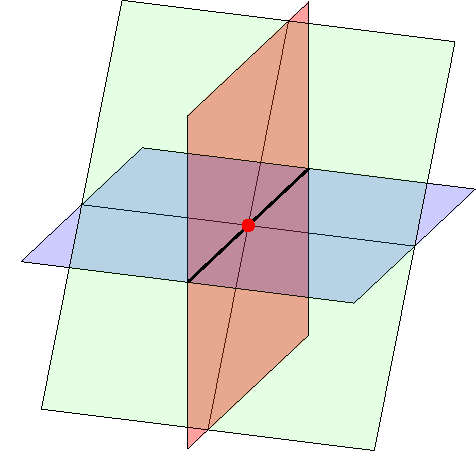
\includegraphics[scale=0.6]{3-planos-solucao-unica.pdf}
                \caption{Solu\c{c}\~ao \'unica}
        \end{figure}
    \item Os tr\^es planos se interceptam em infinitos pontos. Existem infinitos valores de $x$, $y$, $z \in \cp{K}$ que satisfazem as tr\^es equa\c{c}\~oes simultanemente. Neste caso dizemos que o sistema \eqref{sistema_linear_3x3} \'e \textbf{poss{\'\i}vel e indeterminado}.
        \begin{figure}[h]
            \centering
            \begin{subfigure}{.32\textwidth}
                \centering
                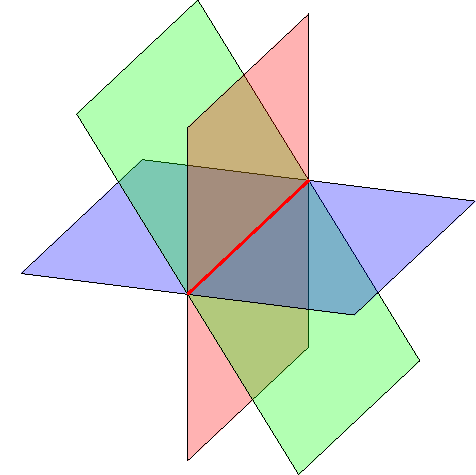
\includegraphics[width=\linewidth]{2-planos-coincidentes-infinitas-solucoes-intersecao-reta.pdf}
                \caption{Infinitas solu\c{c}\~oes}
            \end{subfigure}
            \begin{subfigure}{.32\textwidth}
                \centering
                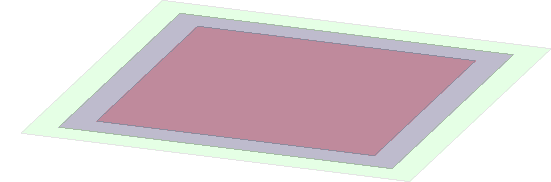
\includegraphics[width=\linewidth]{3-planos-coincidentes-infinitas-solucoes.pdf}
                \caption{Infinitas solu\c{c}\~oes}
            \end{subfigure}
            \begin{subfigure}{.32\textwidth}
                \centering
                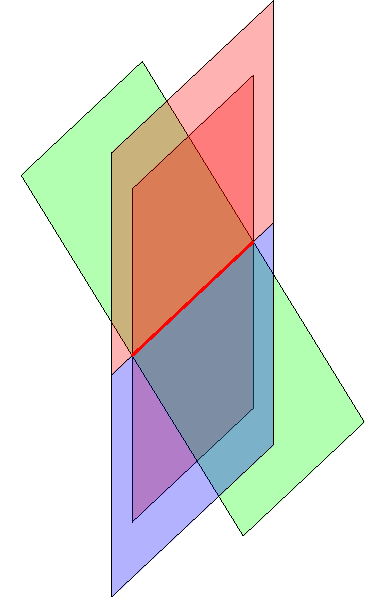
\includegraphics[width=\linewidth]{2-planos-coincidentes-terceiro-fora-infinitas-solucoes-intersecao-reta.pdf}
                \caption{Infinitas solu\c{c}\~oes}
            \end{subfigure}
        \end{figure}
    \item Os tr\^es planos n\~ao possuem uma interse\c{c}\~ao em comum. Neste caso n\~ao existem valores de $x$, $y$, $z \in \cp{K}$  satisfazendo as tr\^es equa\c{c}\~oes simultaneamente. Assim dizemos que o sistema \eqref{sistema_linear_3x3}  \'e \textbf{imposs{\'\i}vel}.
        \begin{figure}[h]
            \centering
            \begin{subfigure}{.32\textwidth}
                \centering
                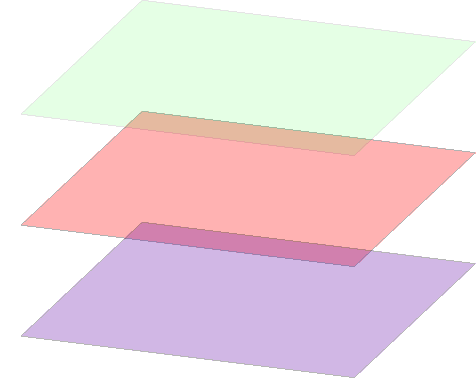
\includegraphics[width=\linewidth]{3-planos-paralelos-nenhuma-solucao.pdf}
                \caption{Nenhuma solu\c{c}\~ao}
            \end{subfigure}
            \begin{subfigure}{.32\textwidth}
                \centering
                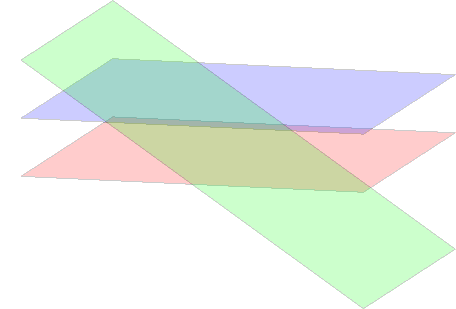
\includegraphics[width=\linewidth]{2-planos-paralelos-nenhuma-solucao.pdf}
                 \caption{Nenhuma solu\c{c}\~ao}
              \end{subfigure}
            \begin{subfigure}{.32\textwidth}
                \centering  
           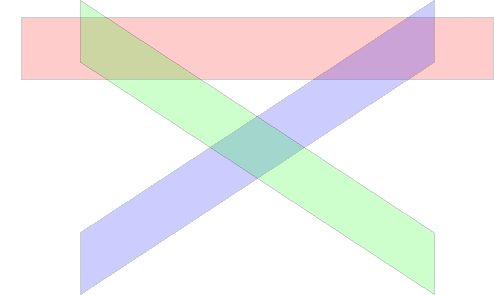
\includegraphics[width=\linewidth]{3-planos-sem-nenhuma-intersecao-dois-a-dois-retas-nenhuma-solucao.pdf}
            \caption{Nenhuma solu\c{c}\~ao}
           \end{subfigure}
        \end{figure}
\end{enumerate}

Agora, de modo geral queremos trabalhar com uma quantidade qualquer de equa\c{c}\~oes. Para isso come\c{c}amos escolhendo escalares $b_1$, \dots, $b_m$  e $a_{ij}$,  $1 \le i \le m$, $1 \le j \le n$ todos em $\cp{K}$.

Queremos saber se \'e poss{\'\i}vel encontrar valores para  $x_1$, $x_2$, \dots, $x_n$  de modo que o seguinte conjunto de equa\c{c}\~oes sejam v\'alidas: 
\begin{equation}\label{sistema_linear_geral}
\begin{cases}
        a_{11}x_1 + a_{12}x_2 + \cdots + a_{1n}x_n = b_1\\
        a_{21}x_1 + a_{22}x_2 + \cdots + a_{2n}x_n = b_2\\
        \qquad \vdots\\
        a_{m1}x_1 + a_{m2}x_2 + \cdots + a_{mn}x_n = b_m
    \end{cases}
\end{equation}

O conjunto de equa\c{c}\~oes em \eqref{sistema_linear_geral} \'e chamado de um  \textbf{sistema de $m$ equa\c{c}\~oes lineares  a $n$ inc\'ognitas}\index{Sistema Linear} $x_1$, $x_2$, \dots, $x_n$ , ou simplesmente de um \textbf{sistema linear}, nas inc\'ognitas  $x_1$, $x_2$, \dots, $x_n$.

Uma solu\c{c}\~ao de um sistema linear do tipo \eqref{sistema_linear_geral}
\[
    x_1 = \alpha_1,  x_2 = \alpha_2,  \dots, x_n = \alpha_n
\]
onde $\alpha_1$, $\alpha_2$, \dots, $\alpha_n \in \cp{K}$,  pode ser escrita como
\[
    (\alpha_1, \alpha_2, \dots, \alpha_n)
\]
e \'e chamada de uma \textbf{\^enupla ordenada}\index{Sistemas linears!\^enupla ordenada} ou uma \textbf{n-upla ordenada}.


Se $b_1 = b_2 = \cdots = b_m = 0_\cp{K} \in K$,  dizemos que o sistema
\begin{equation}\label{sistemalinearhomogeneo}\index{Sistema Linear}
    \begin{cases}
        a_{11}x_1 + a_{12}x_2 + \cdots + a_{1n}x_n = 0_\cp{K}\\
        a_{21}x_1 + a_{22}x_2 + \cdots + a_{2n}x_n = 0_\cp{K}\\
        \qquad \vdots\\
        a_{m1}x_1 + a_{m2}x_2 + \cdots + a_{mn}x_n = 0_\cp{K}
    \end{cases}
\end{equation}
\'e um \textbf{sistema linear homog\^eneo}.\index{Sistema linear!homog\^eneo} 

Observe que tal sistema sempre possui solu\c{c}\~ao,  a saber, $x_1 = x_2 = \cdots = x_n = 0_\cp{K}$.

Para o caso de sistemas lineares temos o seguinte resultado:

\begin{teorema}
    Todo sistema linear do tipo \eqref{sistema_linear_geral} tem zero,  uma  ou uma infinidade de solu\c{c}\~oes.  N\~ao existem outras possibilidades.
\end{teorema}

No caso de um sistema linear da forma \eqref{sistema_linear_geral},  o processo para encontrar suas solu\c{c}\~oes ser\'a feito mediante o uso de 3 tipos de opera\c{c}\~oes.  S\~ao elas:
\begin{itemize}
\item[$e_1$)] Troca da posi\c{c}\~ao de duas equa\c{c}\~oes.
\item[$e_2$)] Multiplica\c{c}\~ao de uma equa\c{c}\~ao por um escalar n\~ao nulo.
\item[$e_3$)] Substitui\c{c}\~ao de uma equa\c{c}\~ao pela soma desta equa\c{c}\~ao com alguma outra.
\end{itemize}

Estas tr\^es opera\c{c}\~oes s\~ao chamadas de  \textbf{opera\c{c}\~oes elementares}.

\begin{exemplos}
    Utilizando somente opera\c{c}\~oes elementares encontre as solu\c{c}\~oes dos seguintes sistemas lineares:
    \begin{enumerate}[label={\arabic*})]
        \item $\begin{cases}x + y = 4\\3x + 3y = 6\end{cases}$

        \item $\begin{cases}x + y + 2z = 9\\ 2x + 4y - 3z = 1\\ 3x + 6y - 3z = 0\end{cases}$
    \end{enumerate}

    \begin{solucao}
        \begin{enumerate}[label={\arabic*})]
            \item Neste caso podemos somar a segunda equa\c{c}\~ao do sistema com ela mesma mais -3 vezes a primeira equa\c{c}\~ao:
                \[
                    \begin{cases}
                        x + y = 4\\
                        3x + 3y + (-3x) + (-3y) = 4 + (-3)\cdot 4
                    \end{cases}
                \]
            que resulta em
            \[
                \begin{cases}
                    x + y = 4\\
                    0 = -6
                \end{cases}
            \]
            e a segunda equa\c{c}\~ao desse sistema \'e uma contradi\c{c}\~ao. Logo n\~ao existem valores para $x$ e $y$ em $\real$ que satisfazem as duas equa\c{c}\~oes desse sistema simultaneamente. Portanto tal sistema \'e um \textbf{sistema imposs{\'\i}vel}.
                    \item Denote as linhas desse sistema por $L_1$, $L_2$ e $L_3$. Come\c{c}amos trocando a linha 2, $L_2$, por ela mesma somanda com -2 vezes a linha 1, $L_1$. Denotemos essa opera\c{c}\~ao por $L_2 \to L_2 - 2L_1$. Com essa opera\c{c}\~ao obtemos o sistema
                        \[
                            \begin{cases}
                                x + y + 2z = 9\\
                                2y - 7z = -17\\
                                3x + 6y - 3z = 0
                            \end{cases}
                        \]
                        Agora trocamos a linha 3 por ela mesma menos 3 vezes a linha 1 ($L_3 \to L_3 - 3L_1$). Ap\'os essa opera\c{c}\~ao o sistema anterior torna-se
                        \[
                            \begin{cases}
                                x + y + 2z = 9\\
                                2y - 7z = -17\\
                                3y - 9z = -27
                            \end{cases}
                        \]
                        Multiplicando a segunda linha por 1/2 ($L_2 \to \frac{1}{2}L_2$) obtemos:
                        \[
                            \begin{cases}
                                x + y + 2z = 9\\
                                y - (7/2)z = -17/2\\
                                3y - 9z = -27
                            \end{cases}
                        \]
                        Agora vamos multiplicar a segunda linha por -3 e somar com a terceira linha ($L_3 \to L_3 - 3L_2$).
                        \[
                            \begin{cases}
                                x + y + 2z = 9\\
                                y - (7/2)z = -17/2\\
                                3/2z = -3/2
                            \end{cases}
                        \]
                        Podemos multiplicar a terceira linha por 2/3 ($L_3 \to \dfrac{2}{3}L_3$) para obter:
                        \[
                            \begin{cases}
                                x + y + 2z = 9\\
                                y - (7/2)z = -17/2\\
                                z = -1
                            \end{cases}
                        \]
                        Troque a primeira linha por ela mesma menos a segunda linha ($L_1 \to L_1 - L_2$):
                        \[
                            \begin{cases}
                                x + (11/2)z = 35/2\\
                                y - (7/2)z = -17/2\\
                                z = -1
                            \end{cases}
                        \]
                        Agora trocamos a segunda linha por ela mesma mais 7/2 vezes a terceira linha ($L_2 \to L_2 + (7/2)L_3$):
                        \[
                            \begin{cases}
                                x + (11/2)z = 35/2\\
                                y  = -12\\
                                z = -1
                            \end{cases}
                        \]
                        Finalmente, trocando a primeira linha por ela mesma menos (11/2) vezes a terceira linha ($L_1 \to L_1 - (11/2)L_3$) obtemos
                        \[
                            \begin{cases}
                                x = 23\\
                                y = -12\\
                                z = -1
                            \end{cases}
                        \]
                        Assim vemos que o sistema tem uma \'unica solu\c{c}\~ao que \'e $x = 23$, $y = -12$ e $z = -1$.
        \end{enumerate}
    \end{solucao}
\end{exemplos}

Observe nos exemplos anteriores que a aplica\c{c}\~ao das opera\c{c}\~oes elementares afeta somente os coeficientes das vari\'aveis e os termos independentes. As vari\'aveis do sistema permanecem inalteradas durante todo o processo. Assim n\~ao precisamos ficar repetindo as vari\'aveis o tempo todo. Podemos tratar somente com seus coeficientes e os termos independetes do sistema.

A partir dessa observa\c{c}\~ao, podemos associar ao sistema \eqref{sistema_linear_geral} uma matriz contendo os coeficientes de cada equa\c{c}\~ao junto com seus respectivos termos independentes. Obtemos assim a matriz
\[
\begin{bmatrix}
        a_{11} & a_{12} & \cdots & a_{1n} & b_1\\
a_{21} & a_{22} & \cdots & a_{2n} & b_2\\
\vdots & \vdots & \vdots & \vdots & \vdots\\
a_{m1} & a_{m2} & \cdots & a_{mn} & b_m\\
    \end{bmatrix}
\]

que \'e chamada de \textbf{matriz ampliada do sistema}  ou \textbf{matriz aumentada do sistema}.

Para destacar que a \'ultima coluna dessa matriz cont\'em os termos independentes do sistema podemos tamb\'em escrever:
\[
    \begin{amatrix}{4}
        a_{11} & a_{12} & \cdots & a_{1n} & b_1\\
    a_{21} & a_{22} & \cdots & a_{2n} & b_2\\
    \vdots & \vdots & \vdots & \vdots & \vdots\\
    a_{m1} & a_{m2} & \cdots & a_{mn} & b_m\\
    \end{amatrix}
\]

\begin{exemplos}
    Escreva a matriz ampliada dos seguintes sistemas lineares:
    \begin{enumerate}[label={\arabic*})]
        \item \[\begin{cases} x_1 + x_2 - 3x_3 + x_4 = -1\\ 2x_1 - 3x_2 + x_4 = 0\\ 3x_1 + 2x_3 = -3\\ x_1 + x_4 = -2\end{cases}\]
        \item \[\begin{cases} x_1 + x_2 - 3x_3 + x_4 = -2\\ 2x_1 - 3x_2 + x_4 = 0\end{cases}\]
        \item \[\begin{cases} 2x_1 - 5x_2 + 4x_3 - 7x_4 + 8x_5 = 0\\ 3x_1 - 7x_2 + 2x_4 - 9x_5 = 0\\ 5x_3 + 8x_4 = 0\\ x_3 - x_4 = 0\end{cases}\]
    \end{enumerate}
    \begin{solucao}
        \begin{enumerate}[label={\arabic*})]
            \item Neste caso a matriz ampliada \'e:
                \[
                    \begin{amatrix}{4}
                        1 & 1 & -3 & 1 & -1\\
                        2 & -3 & 0 & 1 & 0\\
                        3 & 0 & 2 & 0 & -3\\
                        1 & 0 & 0 & 1 & -2
                    \end{amatrix}
                \]
            \item Neste caso a matriz ampliada \'e:
                \[
                    \begin{amatrix}{4}
                        1 & 1 & -3 & 1 & -2\\
                        2 & -3 & 0 & 1 & 0\\
                    \end{amatrix}
                \]
            \item Neste caso a matriz ampliada \'e:
                \[
                    \begin{amatrix}{5}
                        2 & -5 & 4 & -7 & 8 & 0\\
                        3 & -7 & 0 & 2 & -9 & 0\\
                        0 & 0 & 5 & 8 & 0 & 0\\
                        0 & 0 & 1 & -1 & 0 & 0
                    \end{amatrix}
                \]
                Como a \'ultima coluna dessa matriz \'e composta somente de zeros podemos omit{\'\i}-la e escrever:
                \[
                    \begin{bmatrix}
                        2 & -5 & 4 & -7 & 8\\
                        3 & -7 & 0 & 2 & -9\\
                        0 & 0 & 5 & 8 & 0\\
                        0 & 0 & 1 & -1 & 0 
                    \end{bmatrix}
                \]

        \end{enumerate}
    \end{solucao}
\end{exemplos}
Na forma matricial as opera\c{c}\~oes elementares s\~ao descritas como:

\vspace{.3cm}

\begin{itemize}
    \item[$e_1$)] Trocar a $i$-\'esima linha de $A$ pela $j$-\'esima linha de $A$: $L_i \leftrightarrow L_j$;

    \item[$e_2$)] Multiplica\c{c}\~ao da $i$-\'esima linha de $A$ por um escalar $\alpha \in \cp{K}$ n\~ao nulo: $L_i \rightarrow \alpha L_i$;

   \item[$e_3$)] Substitui\c{c}\~ao da $i$-\'esima linha de $A$ pela $i$-\'esima linha mais $\alpha$ vezes a $j$-\'esima linha: $L_i \rightarrow L_i + \alpha L_j$.
\end{itemize}

O que iremos fazer para resolver um sistema linear do tipo \eqref{sistema_linear_geral} \'e aplicar opera\c{c}\~oes opera\c{c}\~oes elementares na linhas da matriz ampliada at\'e que ela esteja num formato especial. Esse formato que buscamos \'e o seguinte:

\begin{definicao}\label{linhareduzida}
    Uma matriz $A$ $m \times n$ \'e  dita estar na \textbf{forma escalonada reduzida por linhas} se:
    \begin{enumerate}[label={\roman*})]
        \item O primeiro elemento n\~ao nulo em cada linha n\~ao nula de $A$ \'e $1$. Dizemos que esse n\'umero 1 \'e um \textbf{piv\^o}.

        \item Toda linha de $A$ cujos elementos s\~ao todos nulos ocorre abaixo de todas as linhas que possuem um elemento n\~ao-nulo. 

        \item Se as linhas 1, 2, \dots, $r$ s\~ao as linhas n\~ao-nulas de $A$ e se o \textbf{piv\^o} da linha $i$ ocorre na coluna $k_i$, $i = 1$, \dots, $r$, ent\~ao $k_1 < k_2 < \cdots < k_r$.

        \item Cada coluna de $A$ que cont\'em um \textbf{piv\^o} tem todos os seus outros elementos nulos.
    \end{enumerate}
\end{definicao}

\begin{observacao}
    Uma matriz que satisfaz as tr\^es primeiras propriedades da defini\c{c}\~ao anterior \'e dita estar na \textbf{forma escalonada por linhas}, ou simplesmente, em \textbf{forma escalonada}.
\end{observacao}

\begin{exemplos}
    \begin{enumerate}[label={\arabic*})]
        \item As seguintes matrizes est\~ao na \textbf{forma escalonada reduzida por linhas}:
            \begin{align*}
                \begin{bmatrix}
                    1 & 0 & 0 & 4\\
                    0 & 1 & 0 & 7\\
                    0 & 0 & 1 & 1
                \end{bmatrix};
                \begin{bmatrix}
                    0 & 1 & i & 3 & 3\\
                    0 & 0 & 0 & 1 & -2 + 4i\\
                    0 & 0 & 0 & 0 & 0
                \end{bmatrix};
                \begin{bmatrix}
                    0 & 0\\
                    0 & 0
                \end{bmatrix};
                \begin{bmatrix}
                    1 & 0 & 0\\
                    0 & 1 & 0\\
                    0 & 0 & 1
                \end{bmatrix}.
            \end{align*}

        \item J\'a as seguintes matrizes est\~ao na \textbf{forma escalonada}:
            \begin{align*}
                \begin{bmatrix}
                    1 & 4 & -3 & 7\\
                    0 & 1 & 6 & 2\\
                    0 & 0 & 1 & 5
                \end{bmatrix};
                \begin{bmatrix}
                    1 & 1 & 0\\
                    0 & 1 & 0\\
                    0 & 0 & 0
                \end{bmatrix};
                \begin{bmatrix}
                    0 & 1 & 2 & 3 & 0\\
                    0 & 0 & 0 & 1 & 1\\
                    0 & 0 & 0 & 0 & 1
                \end{bmatrix}.
            \end{align*}
        \item Usando a matriz ampliada e as opera\c{c}\~oes elementares sobre as linhas da matriz resolva o seguinte sistema:
            \[
                \begin{cases}
                    2x_1 - 4x_2 - x_3 = 1\\
                    x_1 - 3x_2 + x_3 = 1\\
                    3x_1 - 5x_2 - 3x_3 = 1
                \end{cases}
            \]
            \begin{solucao}
                Come\c{c}amos montando a matriz ampliada do sistema:
                \[
                    \begin{amatrix}{3}
                    2 & -4 & -1 & 1\\
                1 & -3 & 1 & 1\\
                3 & -5 & -3 & 1
                    \end{amatrix}.
                \]
                Vamos aplicar as opera\c{c}\~oes elementares nessa matriz:
                \begin{align*}
                    &\begin{bmatrix}
                        2 & -4 & -1 & 1\\
                1 & -3 & 1 & 1\\
                3 & -5 & -3 & 1
                    \end{bmatrix}
                    \begin{array}{l}
                        L_1 \leftrightarrow L_2\\\phantom{x} \\\phantom{x} 
                    \end{array} \sim
                    \begin{bmatrix}
                1 & -3 & 1 & 1\\
                        2 & -4 & -1 & 1\\
                3 & -5 & -3 & 1
                    \end{bmatrix}
                    \begin{array}{l}
                        \phantom{x}\\  L_2 \to L_2 - 2L_1\\\phantom{x}
                    \end{array} \sim\\
                    &\begin{bmatrix}
                1 & -3 & 1 & 1\\
                        0 & 2 & -3 & -1\\
                3 & -5 & -3 & 1
                    \end{bmatrix}
                    \begin{array}{l}
                        \phantom{x}\\ \phantom{x}\\ L_3 \to L_3 - 3L_1
                    \end{array} \sim
                    \begin{bmatrix}
                1 & -3 & 1 & 1\\
                        0 & 2 & -3 & -1\\
                0 & 4 & -6 & -2
                    \end{bmatrix}
                    \begin{array}{l}
                        \phantom{x}\\ \phantom{x}\\ L_3 \to L_3 - 2L_1
                    \end{array} \sim\\
                    &\begin{bmatrix}
                1 & -3 & 1 & 1\\
                        0 & 2 & -3 & -1\\
                0 & 0 & 0 & 0
                    \end{bmatrix}
                    \begin{array}{l}
                        \phantom{x}\\ L_2 \to \dfrac{1}{2}L_2\\\phantom{x}
                    \end{array} \sim
                    \begin{bmatrix}
                1 & -3 & 1 & 1\\
                        0 & 1 & -3/2 & -1/2\\
                0 & 0 & 0 & 0
                    \end{bmatrix}
                    \begin{array}{l}
                        L_1 \to L_1 + 3L_2\\\phantom{x}\\\phantom{x}
                    \end{array} \sim\\
                    &\begin{bmatrix}
                1 & 0 & -7/2 & -1/2\\
                        0 & 1 & -3/2 & -1/2\\
                0 & 0 & 0 & 0
                    \end{bmatrix}
                \end{align*}
                Essa \'ultima matriz est\'a na forma escalonada reduzida por linhas. Assim obtemos o sistema
                \[
                    \begin{cases}
                        x_1 - (7/2)x_3 = -1/2\\
                        x_2 - (3/2)x_3 = -1/2
                    \end{cases}.
                \]

                Desse sistema obtemos
                \[
                    x_2 = -\dfrac{1}{2} + \dfrac{3}{2}x_3
                \]
                e substituindo essa equa\c{c}\~ao na primeira encontramos
                \[
                    x_1 = -\dfrac{1}{2} + \dfrac{7}{2}x_3.
                \]
                Portanto fazendo $x_3 = t \in \real$ a solu\c{c}\~ao desse sistema pode ser escrita como
                \[
                    x_1 = -\dfrac{1}{2} + \dfrac{7}{2}t, x_2 = -\dfrac{1}{2} + \dfrac{3}{2}t, x_3 = t, t \in \real.
                \]
                Logo o sistema \'e poss{\'\i}vel e indeterminado.
            \end{solucao}
    \end{enumerate}
\end{exemplos}
    
\begin{definicao}
    Se $A$ e $B$ s\~ao matrizes $m \times n$, dizemos que $B$ \'e \textbf{linha-equivalente}\index{Matrizes!linha-equivalente} a $A$, se $B$ for obtida de $A$ atrav\'es de uma quantidade finita de opera\c{c}\~oes elementares sobre as linhas de $A$.
\end{definicao}

\begin{notacao}
    $A \rightarrow B$ ou $A \sim B$.
\end{notacao}

\begin{exemplos}
    \begin{enumerate}[label={\arabic*})]
        \item As matrizes
            \[
                A = \begin{pmatrix}
                        1 & 2 & -1 & 0\\
                        0 & 1 & 3 & 4\\
                        2 & 0 & 1 & 3
                    \end{pmatrix}
                    \mbox{ e }
                B = \begin{pmatrix}
                        0 & 1 & 3 & 4\\
                        1 & 2 & -1 & 0\\
                        2 & 0 & 1 & 3
                    \end{pmatrix}
            \]
            s\~ao matrizes linha-equivalentes pois podemos obter a matriz $B$ de $A$ trocando a primeira linha de $A$ com a segunda linha. Assim $B \sim A$.
            
            Observe que tamb\'em podemos obter a matriz $A$ a partir de $B$ simplesmente trocando a primeira linha de $B$ com a segunda linha. Logo $A \sim B$.
        \item As matrizes
            \[
                C = \begin{pmatrix}
                        1 & 0 & 3 & 0\\
                        2 & 1 & 0 & 1\\
                        -1 & 3 & 2 & 1
                    \end{pmatrix}
                    \mbox{ e }
                D = \begin{pmatrix}
                        1 & 0 & 3 & 0\\
                        4 & 1 & 6 & 1\\
                        0 & 3 & 5 & 1
                    \end{pmatrix}
            \]
            tamb\'em s\~ao linha-equivalentes. De fato, partindo de $C$ podemos efetuar as seguintes opera\c{c}\~oes elementares:
            \begin{align*}
                C &= \begin{pmatrix}
                    1 & 0 & 3 & 0\\
                    2 & 1 & 0 & 1\\
                    -1 & 3 & 2 & 1
                \end{pmatrix}
                \begin{array}{l}
                    \phantom{x}\\ L_2 \to L_2 + 2L_1\\\phantom{x}
                \end{array} \sim
                \begin{pmatrix}
                    1 & 0 & 3 & 0\\
                    4 & 1 & 6 & 1\\
                    -1 & 3 & 2 & 1
                \end{pmatrix}
                \begin{array}{l}
                    \phantom{x}\\ \phantom{x}\\ L_3 \to L_2 + L_1
                \end{array}\\ \sim
                  &\begin{pmatrix}
                    1 & 0 & 3 & 0\\
                    4 & 1 & 6 & 1\\
                    0 & 3 & 5 & 1
                \end{pmatrix} = D
            \end{align*}
            Assim $D \sim C$.

            Poder{\'\i}amos fazer o contr\'ario, come\c{c}ar de $D$ e obter a matriz $C$:
            \begin{align*}
                D &= \begin{pmatrix}
                    1 & 0 & 3 & 0\\
                    4 & 1 & 6 & 1\\
                    0 & 3 & 5 & 1
                \end{pmatrix}
                \begin{array}{l}
                    \phantom{x}\\ L_2 \to L_2 - 2L_1\\\phantom{x}
                \end{array} \sim
                \begin{pmatrix}
                    1 & 0 & 3 & 0\\
                    2 & 1 & 0 & 1\\
                    0 & 3 & 5 & 1
                \end{pmatrix}
                \begin{array}{l}
                    \phantom{x}\\ \phantom{x}\\ L_3 \to L_3 - L_1
                \end{array}\\ \sim
                  &\begin{pmatrix}
                    1 & 0 & 3 & 0\\
                    2 & 1 & 0 & 1\\
                    -1 & 3 & 2 & 1
                \end{pmatrix} = C
            \end{align*}

            Assim $C \sim D$.
    \end{enumerate}
\end{exemplos}
\begin{teorema}
    Duas matrizes $A$ e $B$ s\~ao equivalentes por linha se, e somente, se elas puderem ser reduzidas \`a mesma forma escalonada por linhas.
\end{teorema}

\begin{teorema}
    Se as matrizes ampliadas de dois sistemas lineares s\~ao equivalentes por linhas, ent\~ao os dois sistemas possuem as mesmas solu\c{c}\~oes.
\end{teorema}

O \textbf{m\'etodo de elimina\c{c}\~ao de Gauss}\index{Sistemas lineares!m\'etodo de elimina\c{c}\~ao de Gauss} ou \textbf{m\'etodo de elemina\c{c}\~ao gaussiana}\index{Sistemas lineares!elimina\c{c}\~ao gaussiana} consiste em substituir um dado sistema de equa\c{c}\~oes lineares  por outro \textbf{equivalente}, que seja mais simples de ser solucionado e que tenha a mesma solu\c{c}\~ao do sistema original.

\begin{definicao}[M\'etodo de elimina\c{c}ao de Gauss]
    Seja $A$ a matriz ampliada de um sistema linear. O m\'etodo de \textbf{elimina\c{c}\~ao de Gauss} consiste em:
    \begin{enumerate}[label={\roman*})]
        \item Escreva a matriz ampliada do sistema de equa\c{c}\~oes lineares.

        \item Use opera\c{c}\~oes elementares nas linhas de $A$ para reduzir a matriz ampliada \`a \textbf{forma escalonada por linhas}.
        
        \item Quando a matriz ampliada estiver na forma escalonada, usando substitui\c{c}\~ao de tr\'as para a frente, resolva o sistema equivalente que corresponde a matriz escalonada reduzida por linhas.
    \end{enumerate}
\end{definicao}

\begin{observacao}
    No momento de aplicar o passo 2 do m\'etodo de elimina\c{c}\~ao de Guass, temos v\'arias escolhas que podemos fazer. Algumas dicas para a escolha da opera\c{c}\~ao s\~ao as seguintes:
    \begin{enumerate}[label=({\alph*})]
        \item Localize a coluna mais \`a esquerda que n\~ao \'e toda formada por zeros.
        
        \item Crie um \textbf{piv\^o} no topo desta coluna.
         
        \item Use o \textbf{piv\^o} para criar zeros abaixo dele.

        \item Fa\c{c}a a linha contendo este \textbf{piv\^o} ir para a parte de cima e volte ao passo (a) para repetir o procedimento com o restante da submatriz. Pare quando toda a matriz estiver na forma escalonada por linhas.
    \end{enumerate}
\end{observacao}

\begin{exemplos}
    \begin{enumerate}[label={\arabic*})]
        \item Encontre a solu\c{c}\~ao do seguinte sistema em $\rac$:
        \[
            \begin{cases}
                6x_3 + 19x_5 + 11x_6 = -27\\
                3x_1 + 12x_2 + 9x_3 - 6x_4 + 26x_5 + 31x_6 = -63\\
                x_1 + 4x_2 + 3x_3 - 2x_4 + 10x_5 + 9x_6 = -17\\
                -x_1 - 4x_2 - 4x_3 + 2x_4 - 13x_5 - 11x_6 = 22
            \end{cases}
        \]
        \item Considere o seguinte sistema em $\real$:
        \[
            \begin{cases}
                2x_1 + 4x_5 = 16\\
                5x_1 - 2x_2 = 4\\
                10x_1 - 4x_2 = 3
            \end{cases}
        \]
        \item Estude o seguinte sistema linear:
        \[
            \begin{cases}
                x_1 - x_2 + kx_3 = 1\\
                2x_1 + x_2 + x_3 = 0\\
                x_1 + 2x_2 + (1 - k)x_3 = k
            \end{cases}
        \]
        onde $k \in \real$. Isto \'e, decida para quais valores de $k \in \real$ esse sistema admite solu\c{c}\~ao \'unica, infinitas solu\c{c}\~oes e nenhuma solu\c{c}\~ao.
    \end{enumerate}
    \begin{solucao}
        \begin{enumerate}
            \item Primeiro montamos a matriz ampliada do sistema:
            \[
                \begin{amatrix}{6}
                    0 & 0 & 6 & 0 & 19 & 11 & -27\\
                    3 & 12 & 9 & -6 & 26 & 31 & -63\\
                    1 & 4 & 3 & -2 & 10 & 9 & -17\\
                    -1 & -4 & -4 & 2 & -13 & -11 & 22
                \end{amatrix}
            \]
            O primeiro passo e colocar um piv\^o na primeira linha. Para isso podemos trocar as linhas 1 e 3 de posi\c{c}\~ao: $L_1 \leftrightarrow L_3$:
            \[
               \begin{amatrix}{6}
                    1 & 4 & 3 & -2 & 10 & 9 & -17\\
                    3 & 12 & 9 & -6 & 26 & 31 & -63\\
                    0 & 0 & 6 & 0 & 19 & 11 & -27\\
                    -1 & -4 & -4 & 2 & -13 & -11 & 22
               \end{amatrix}
            \]
            Agora vamos zerar todos os elementos na primeira coluna abaixo do 1:
            \begin{align*}
                &\begin{amatrix}{6}
                    1 & 4 & 3 & -2 & 10 & 9 & -17\\
                    3 & 12 & 9 & -6 & 26 & 31 & -63\\
                    0 & 0 & 6 & 0 & 19 & 11 & -27\\
                    -1 & -4 & -4 & 2 & -13 & -11 & 22
                \end{amatrix}
                \begin{array}{l}
                    \phantom{x}\\L_2 \to L_2 - 3L_1\\\phantom{x}\\L_4 \to L_4 + L_1
                \end{array}\sim\\
                &\begin{amatrix}{6}
                    1 & 4 & 3 & -2 & 10 & 9 & -17\\
                    0 & 0 & 0 & 0 & -4 & 4 & -12\\
                    0 & 0 & 6 & 0 & 19 & 11 & -27\\
                    0 & 0 & -1 & 0 & -3 & -2 & 5
                \end{amatrix}
            \end{align*}
            Na quarta linha temos um -1 na terceira coluna. Por isso, podemos trocar a segunda e a quarta linhas de posi\c{c}\~ao: $L_2 \leftrightarrow L_4$
            \[
                \begin{amatrix}{6}
                    1 & 4 & 3 & -2 & 10 & 9 & -17\\
                    0 & 0 & -1 & 0 & -3 & -2 & 5\\
                    0 & 0 & 6 & 0 & 19 & 11 & -27\\
                    0 & 0 & 0 & 0 & -4 & 4 & -12
                \end{amatrix}
            \]
            Multiplicamos a segunda linha por -1 para obter um piv\^o na terceira coluna:
            \[
                \begin{amatrix}{6}
                    1 & 4 & 3 & -2 & 10 & 9 & -17\\
                    0 & 0 & 1 & 0 & 3 & 2 & -5\\
                    0 & 0 & 6 & 0 & 19 & 11 & -27\\
                    0 & 0 & 0 & 0 & -4 & 4 & -12
                \end{amatrix}
            \]
            Agora vamos zerar todos os coeficientes que est\~ao na terceira coluna e abaixo do piv\^o:
            \begin{align*}
                &\begin{amatrix}{6}
                    1 & 4 & 3 & -2 & 10 & 9 & -17\\
                    0 & 0 & 1 & 0 & 3 & 2 & -5\\
                    0 & 0 & 6 & 0 & 19 & 11 & -27\\
                    0 & 0 & 0 & 0 & -4 & 4 & -12
                \end{amatrix}
                \begin{array}{l}
                    \phantom{x}\\ \phantom{x}\\ L_3 \to L_3 - 6L_2\\ \phantom{x} 
                \end{array}\sim\\
                &\begin{amatrix}{6}
                    1 & 4 & 3 & -2 & 10 & 9 & -17\\
                    0 & 0 & 1 & 0 & 3 & 2 & -5\\
                    0 & 0 & 0 & 0 & 1 & -1 & 3\\
                    0 & 0 & 0 & 0 & -4 & 4 & -12
                \end{amatrix}
            \end{align*}
            Como na terceira linha j\'a temos um piv\^o na quinta coluna, vamos somente zerar os coeficientes abaixo desse piv\^o.
            \begin{align*}
                &\begin{amatrix}{6}
                    1 & 4 & 3 & -2 & 10 & 9 & -17\\
                    0 & 0 & 1 & 0 & 3 & 2 & -5\\
                    0 & 0 & 0 & 0 & 1 & -1 & 3\\
                    0 & 0 & 0 & 0 & -4 & 4 & -12
                \end{amatrix}
                \begin{array}{l}
                    \phantom{x}\\ \phantom{x}\\ \phantom{x}\\ L_4 \to L_4 - 4L_3 
                \end{array}\sim\\
                &\begin{amatrix}{6}
                    1 & 4 & 3 & -2 & 10 & 9 & -17\\
                    0 & 0 & 1 & 0 & 3 & 2 & -5\\
                    0 & 0 & 0 & 0 & 1 & -1 & 3\\
                    0 & 0 & 0 & 0 & 0 & 0 & 0
                \end{amatrix}
            \end{align*}
            Como essa matriz est\'a na forma escalonada temos o seguinte sistema:
            \[
                \begin{cases}
                    x_1 + 4x_2 + 3x_3 - 2x_4 + 10x_5 + 9x_6 = -17\\
                    x_3 + 3x_5 + 2x_6 = -5\\
                    x_5 - x_6 = 3
                \end{cases}
            \]
            As vari\'aveis $x_2$, $x_4$ e $x_6$ s\~ao chamadas de \textbf{vari\'aveis livres} do sistema linear pois n\~ao est\~ao associadas a nenhum \textbf{piv\^o} na matriz escalonada desse sistema.
            Da terceira equa\c{c}\~ao temos
            \[
                x_5 = 3 + x_6.
            \]
            Substituindo esse valor na segunda equa\c{c}\~ao:
            \begin{align*}
                x_3 + 3(3 + x_6) + 2x_6 = -5\\
                x_3 + 9 + 3x_6 + 2x_6 = -5\\
                x_3 = -14 - 5x_6
            \end{align*}
            Finalmente, substituindo os valores encontrados para $x_3$ e $x_5$ na primeira equa\c{c}\~ao:
            \begin{align*}
                x_1 + 4x_2 + 3(-14 - 5x_6) - 2x_4 + 10(3 + x_6) + 9x_6 = -17\\
                x_1 + 4x_2 - 42 - 15x_6 - 2x_4 + 30 + 10x_6 + 9x_6 = -17\\
                x_1 = -5 - 4x_2 + 2x_4 - 4x_6
            \end{align*}

            Fazendo $x_2 = s$, $x_4 = t$ e $x_6 = z$ com $s$, $t$ e $z \in \rac$ podemos escrever
            \begin{align*}
                x_1 &= -5 - 4s + 2t - 4z\\
                x_2 &= s\\
                x_3 &= -14 - 5z\\
                x_4 &= t\\
                x_5 &= 3 + z\\
                x_6 &= z
            \end{align*}
            Nesse caso temos um sistema \textbf{poss{\'\i}vel e indeterminado}. O sistema admite infinitas solu\c{c}\~oes. Podemos escrever as solu\c{c}\~oes desse sistema como o conjunto
            \[
                S = \{(-5 - 4s + 2t - 4z, s, -14 - 5z, t, 3 + z, z) \mid s, t, z \in \rac\}
            \]
            que \'e chamado de \textbf{conjunto-solu\c{c}\~ao} do sistema linear.

            \item A matriz ampliada do sistema \'e
                \[
                    \begin{amatrix}{2}
                        2 & 4 & 16\\
                        5 & 2 & 4\\
                        10 & 4 & 3
                    \end{amatrix}
                \]
                Primeiro multiplicamos a linha 1 por 1/2 para termos um piv\^o na primeira coluna:
                \begin{align*}
                    \begin{amatrix}{2}
                        2 & 4 & 16\\
                        5 & 2 & 4\\
                        10 & 4 & 3
                    \end{amatrix}
                    \begin{array}{l}
                        L_1 \to \dfrac{1}{2}L_1\\\phantom{x}\\\phantom{x}
                    \end{array}\sim
                    \begin{amatrix}{2}
                        1 & 2 & 8\\
                        5 & 2 & 4\\
                        10 & 4 & 3
                    \end{amatrix}
                \end{align*}
                Agora vamos zerar os demais coeficientes na primeira coluna:
                \begin{align*}
                    \begin{amatrix}{2}
                        1 & 2 & 8\\
                        5 & 2 & 4\\
                        10 & 4 & 3
                    \end{amatrix}
                    \begin{array}{l}
                        \phantom{x}\\L_2 \to L_2 - 5L_1\\L_3 \to L_3 - 10L_1
                    \end{array}\sim
                    \begin{amatrix}{2}
                        1 & 2 & 8\\
                        0 & -8 & -36\\
                        0 & -16 & -77
                    \end{amatrix}
                \end{align*}
                Agora vamos criar um piv\^o na segunda linha, segunda coluna. Para isso fazemos:
                \begin{align*}
                    \begin{amatrix}{2}
                        1 & 2 & 8\\
                        0 & -8 & -36\\
                        0 & -16 & -77
                    \end{amatrix}
                    \begin{array}{l}
                        \phantom{x}\\L_2 \to -\dfrac{1}{8}\\\phantom{x}
                    \end{array}\sim
                    \begin{amatrix}{2}
                        1 & 2 & 8\\
                        0 & 1 & 9/4\\
                        0 & -16 & -77
                    \end{amatrix}
                \end{align*}
                Por \'ultimo podemos zerar o coeficiente abaixo do piv\^o da segunda linha:
                \begin{align*}
                    \begin{amatrix}{2}
                        1 & 2 & 8\\
                        0 & 1 & 9/4\\
                        0 & -16 & -77
                    \end{amatrix}
                    \begin{array}{l}
                        \phantom{x}\\\phantom{x}\\L_3 \to L_3 + 16L_2!
                    \end{array}\sim
                    \begin{amatrix}{2}
                        1 & 2 & 8\\
                        0 & 1 & 9/4\\
                        0 & 0 & -5
                    \end{amatrix}
                \end{align*}
                Dessa \'ultima matriz, obtemos o sistema
                \[
                    \begin{cases}
                        x_1 - 2x_2 = 8\\
                        x_2 = 3\\
                        0 = -5
                    \end{cases}
                \]
                A \'ultima equa\c{c}\~ao desse sistema n\~ao admite solu\c{c}\~ao. Logo tal sistema \'e imposs{\'\i}vel.
                \item A matriz ampliada desse sistema \'e:
                \[
                    \begin{amatrix}{3}
                        1 & -1 & k & 1\\
                        2 & 1 & 1 & 0\\
                        1 & 2 & 1 - k & k\\
                    \end{amatrix}    
                \]
                Apliquemos a elimina\c{c}\~ao gaussiana
                \begin{align*}
                    &\begin{amatrix}{3}
                        1 & -1 & k & 1\\
                        2 & 1 & 1 & 0\\
                        1 & 2 & 1 - k & k\\
                    \end{amatrix}
                    \begin{array}{l}
                        \phantom{x}\\L_2 \to L_2 - 2L_1\\L_3 \to L_3 - L_1
                    \end{array}\sim
                    \begin{amatrix}{3}
                        1 & -1 & k & 1\\
                        0 & 3 & 1 - 2k & -2\\
                        0 & 3 & 1 - 2k & k - 1\\
                    \end{amatrix}
                    \begin{array}{l}
                        \phantom{x}\\\phantom{x}\\L_3 \to L_3 - L_2
                    \end{array}\\ &\sim
                    \begin{amatrix}{3}
                        1 & -1 & k & 1\\
                        0 & 3 & 1 - 2k & -2\\
                        0 & 0 & 0 & k + 1\\
                    \end{amatrix}
                    \begin{array}{l}
                        \phantom{x}\\L_2 \to \dfrac{1}{3}L_2\\\phantom{x}
                    \end{array}\sim
                    \begin{amatrix}{3}
                        1 & -1 & k & 1\\
                        0 & 1 & (1 - 2k)/3 & -2/3\\
                        0 & 0 & 0 & k + 1\\
                    \end{amatrix}
                \end{align*}
                Da \'ultima linha dessa matriz temos que se $k + 1 \ne 0$, isto \'e, $k \ne -1$ ent\~ao o sistema \'e imposs{\'\i}vel. Ent\~ao para qualquer $K \in \real$ com $k \ne -1$ o sistema \'e imposs{\'\i}vel.

                Se $k = -1$, a \'ultima matriz torna-se
                \[
                    \begin{amatrix}{3}
                        1 & -1 & -1 & 1\\
                        0 & 1 & 1 & -2/3\\
                        0 & 0 & 0 & 0\\
                    \end{amatrix}
                \]
                Com isso obtemos as equa\c{c}\~oes
                \[
                    \begin{cases}
                        x_1 = 1/3\\
                        x_2 + x_3 = -2/3
                    \end{cases}
                \]
                Da segunda equa\c{c}\~ao desse sistema encontramos
                \[
                    x_2 = -\dfrac{2}{3} - x_3
                \]
                Com isso, $x_3$ \'e uma vari\'avel livre. Da{\'\i}, quando $k = -1$ o sistema \'e poss{\'\i}vel e indeterminado. O conjunto-solu\c{c}\~ao \'e
                \[
                    S = \{(1/3, -2/3 - x_3, x_3) \mid x_3 \in \real\}.
                \]
        \end{enumerate}
    \end{solucao}
\end{exemplos}

Considere o sistema linear:
\begin{equation*}
    \begin{cases}
        a_{11}x_1 + a_{12}x_2 + \cdots + a_{1n}x_n = b_1\\
        a_{21}x_1 + a_{22}x_2 + \cdots + a_{2n}x_n = b_2\\
        \qquad \vdots\\
        a_{m1}x_1 + a_{m2}x_2 + \cdots + a_{mn}x_n = b_m
    \end{cases}
\end{equation*}
A matriz
\[
    A = \begin{bmatrix}
        a_{11} & a_{12} & \cdots & a_{1n}\\
        a_{21} & a_{22} & \cdots & a_{2n}\\
        \vdots & \vdots & \cdots & \vdots\\
        a_{m1} & a_{m2} & \cdots & a_{mn}
    \end{bmatrix}
\]
\'e chamada de \textbf{matriz dos coeficientes} do sistema linear.

\begin{definicao}
    Seja $A$ a matriz ampliada de um sistema linear. Se $A$ est\'a na forma escalonada reduzida por linhas, ent\~ao as vari\'aveis desse 
    sistema que n\~ao correspondem aos piv\^os s\~ao chamadas de \textbf{vari\'aveis livres}.\index{Sistemas lineares!vari\'aveis livres}
\end{definicao}

\begin{definicao}
    O \textbf{posto}\index{Matriz!posto}, denotado $\p{A}$ ou $p(A)$, de uma matriz $A$ \'e n\'umero de linhas n\~ao nulas de qualquer 
    uma de suas formas escalonadas por linhas.
\end{definicao}

\begin{teorema}[Teorema do Posto]
    Seja $A$ a matriz dos coeficientes de um sistema linear com $n$ vari\'aveis. Ent\~ao
    \[
        \mbox{n\'umero de vari\'aveis livres} =  n - \p{A}.
    \]
\end{teorema}

Durante a aplica\c{c}\~ao do \textbf{m\'etodo de elimina\c{c}\~ao de Gauss}, paramos quando a matriz ampliada do sistema est\'a na forma escalonada.
Todavia podemos continuar aplicando opera\c{c}\~oes elementares at\'e que a matriz atinja a forma escalonada reduzida por linhas. Esse \'e o caso do 
\textbf{m\'etodo de Gaus-Jordan}.

\begin{definicao}[M\'etodo de elimina\c{c}ao de Gauss-Jordan]
    O m\'etodo de \textbf{elimina\c{c}\~ao de Gauss-Jordan}, para solu\c{c}\~ao de um sistema linear, consiste em:
    \begin{enumerate}[label={\roman*})]
        \item Escreva a matriz ampliada do sistema de equa\c{c}\~oes lineares.

        \item Use opera\c{c}\~oes elementares nas linhas de $A$ para reduzir a matriz ampliada \`a \textbf{forma escalonada reduzida por linhas}.
        
        \item Se o sistema resultante for poss{\'\i}vel, resolva-o para as vari\'aveis dependentes em termos de quaisquer vari\'aveis livres que 
            tenham sobrado.
    \end{enumerate}
\end{definicao}
\begin{exemplo}
    Resolva os seguintes sistemas usando o m\'etodo de Guass-Jordan. Encontre o posto e o n\'umero de vari\'aveis livres:
    \begin{enumerate}
        \item $\begin{cases}
                x_1 + 2x_2 - x_3 = 9\\
                2x_1 - x_2 + x_3 = 0\\
                4x_1 - x_2 + x_3 = 4
            \end{cases}$

        \item $\begin{cases}
                w + x + 2y + z = 0\\
                w - x - y + z = 0\\
                x + y = 0\\
                w + x + z = 0
        \end{cases}$
    \end{enumerate}
    \begin{solucao}
        \begin{enumerate}
            \item A matriz ampliada do sistema \'e
                \[
                    \begin{amatrix}{3}
                        1 & 2 & -1 & 9\\
                        2 & -1 & 1 & 0\\
                        4 & -1 & 1 & 4
                    \end{amatrix}
                \]
                Aplicando om\'etodo de Guass-Jordan \`a essa matriz:
                \begin{align*}
                &\begin{amatrix}{3}
                    1 & 2 & -1 & 9\\
                    2 & -1 & 1 & 0\\
                    4 & -1 & 1 & 4
                \end{amatrix}
                \begin{array}{l}
                    \phantom{x}\\L_2 \to L_2 - 2L_1\\L_3 \to L_3 - 4L_1
                \end{array}\sim
                \begin{amatrix}{3}
                    1 & 2 & -1 & 9\\
                    0 & -5 & 3 & -18\\
                    0 & -9 & 5 & -32
                \end{amatrix}
                \begin{array}{l}
                    \phantom{x}\\L_2 \to -\dfrac{1}{5}L_2 \\\phantom{x}
                \end{array}\sim\\
                &\begin{amatrix}{3}
                    1 & 2 & -1 & 9\\
                    0 & 1 & -3/5 & 18/5\\
                    0 & -9 & 5 & -32
                \end{amatrix}
                \begin{array}{l}
                    \phantom{x}\\\phantom{x}\\L_3 \to L_3 + 9L_2
                \end{array}\sim
                \begin{amatrix}{3}
                    1 & 2 & -1 & 9\\
                    0 & 1 & -3/5 & 18/5\\
                    0 & 0 & -2/5 & 2/5
                \end{amatrix}
                \begin{array}{l}
                    \phantom{x}\\\phantom{x}\\L_3 \to -\dfrac{5}{2}L_3
                \end{array}\sim\\
                &\begin{amatrix}{3}
                    1 & 2 & -1 & 9\\
                    0 & 1 & -3/5 & 18/5\\
                    0 & 0 & 1 & -1
                \end{amatrix}
                \begin{array}{l}
                    \phantom{x}\\L_2 \to L_2 +\dfrac{3}{5}L_3\\\phantom{x}\\\phantom{x}
                \end{array}\sim
                \begin{amatrix}{3}
                    1 & 2 & -1 & 9\\
                    0 & 1 & 0 & 3\\
                    0 & 0 & 1 & -1
                \end{amatrix}
                \begin{array}{l}
                    L_1 \to L_1 - 2L_2\\\phantom{x}\\\phantom{x}
                \end{array}\sim\\
                &\begin{amatrix}{3}
                    1 & 0 & -1 & 3\\
                    0 & 1 & 0 & 3\\
                    0 & 0 & 1 & -1
                \end{amatrix}
                \begin{array}{l}
                    L_1 \to L_1 + L_3\\\phantom{x}\\\phantom{x}
                \end{array}\sim
                \begin{amatrix}{3}
                    1 & 0 & 0 & 2\\
                    0 & 1 & 0 & 3\\
                    0 & 0 & 1 & -1
                \end{amatrix}
            \end{align*}
            Assim o posto da matriz \'e 3 e o n\'umero de vari\'aveis livres \'e 0.
            O sistema admite solu\c{c}\~ao \'unica $x_1 = 2$, $x_2 = 3$ e $x_3 = -1$, que pode ser denotada como $S = \{(2,3,-1)\}$.

            \item A matriz ampliada do sistema \'e
                \[
                    \begin{amatrix}{4}
                        1 & 1 & 2 & 1 & 0\\
                        1 & -1 & -1 & 1 & 0\\
                        0 & 1 & 1 & 0 & 0\\
                        1 & 1 & 0 & 1 & 0
                    \end{amatrix}.
                \]
            Como a \'ultima coluna dessa matriz \'e nula podemos omit{\'\i}-la na hora de aplicar o m\'etodo de Gauss-Jordan.
            \begin{align*}
                &\begin{pmatrix}
                    1 &\phantom{-} 1 &\phantom{-} 2 & 1\\
                    1 & -1 & -1 & 1\\
                    0 &\phantom{-} 1 &\phantom{-} 1 & 0\\
                    1 &\phantom{-} 1 &\phantom{-} 0 & 1
                \end{pmatrix}
                \begin{array}{l}
                    \phantom{x}\\L_2 \to L_2 - L_1\\\phantom{x}\\L_4 \to L_4 - L_1
                \end{array}\sim
                \begin{pmatrix}
                    1 &\phantom{-} 1 &\phantom{-} 2 & 1\\
                    0 & -2 & -3 & 1\\
                    0 &\phantom{-} 1 &\phantom{-} 1 & 0\\
                    0 &\phantom{-} 0 & -2 & 0
                \end{pmatrix}
                \begin{array}{l}
                    \phantom{x}\\L_2 \leftrightarrow L_3\\\phantom{x}\\\phantom{x}
                \end{array}\sim\\
                &\begin{pmatrix}
                    1 &\phantom{-} 1 &\phantom{-} 2 & 1\\
                    0 &\phantom{-} 1 &\phantom{-} 1 & 0\\
                    0 & -2 & -3 & 0\\
                    0 &\phantom{-} 0 & -2 & 0
                \end{pmatrix}
                \begin{array}{l}
                    L_1 \to L_1 - L_2\\\phantom{x}\\L_3 \to L_3 + 2L_2\\\phantom{x}
                \end{array}\sim
                \begin{pmatrix}
                    1 & 0 &\phantom{-} 1 & 1\\
                    0 & 1 &\phantom{-} 1 & 0\\
                    0 & 0 & -1 & 0\\
                    0 & 0 & -2 & 0
                \end{pmatrix}
                \begin{array}{l}
                    \phantom{x}\\\phantom{x}\\L_3 \to -L_3\\\phantom{x}
                \end{array}\sim\\
                &\begin{pmatrix}
                    1 & 0 &\phantom{-} 1 & 1\\
                    0 & 1 &\phantom{-} 1 & 0\\
                    0 & 0 &\phantom{-} 1 & 0\\
                    0 & 0 & -2 & 0
                \end{pmatrix}
                \begin{array}{l}
                    L_1 \to L_1 - L_3\\L_2 \to L_2 - L_3\\\phantom{x}\\L_4 \to L_4 + 2L_3
                \end{array}\sim
                \begin{pmatrix}
                    1 & 0 & 0 & 1\\
                    0 & 1 & 0 & 0\\
                    0 & 0 & 1 & 0\\
                    0 & 0 & 0 & 0
                \end{pmatrix}
            \end{align*}
            Neste caso o posto \'e 3 e o n\'umero de vari\'aveis livres \'e 1. A solu\c{c}\~ao desse sistema \'e
            \[
                x_2 = x_3 = 0, x_1 = -x_4
            \]
            que pode ser dada pelo conjunto
            \[
                S = \{(-x_4, 0, 0, x_4) \mid x_4 \in \real\}.
            \]

    \end{enumerate}
\end{solucao}
\end{exemplo}
\begin{teorema}
    Um sistema linear homog\^eneo com mais inc\'ognitas que equa\c{c}\~oes tem uma infinidade de solu\c{c}\~oes.
\end{teorema}

\section{Matriz Inversa}

\begin{definicao}
    Seja $A$ uma matriz quadrada de ordem $n$ e $A \ne 0$. Se for poss{\'\i}vel encontrar uma matriz quadrada $B$ tamb\'em de 
    ordem $n$ tal que
    \[
        AB = I_n = BA   
    \]
    onde $I_n$ \'e a matriz identidade de ordem $n$, ent\~ao diremos que $A$ \'e \textbf{invert{\'\i}vel}, ou \textbf{n\~ao singular},
    e que $B$ \'e a \textbf{inversa} de $A$. Se n\~ao pudermos encontrar tal matriz $B$, ent\~ao diremos que $A$ \'e \textbf{n\~ao invert{\'\i}vel}  
    ou \textbf{singular}.
\end{definicao}

\begin{exemplos}
\begin{enumerate}
    \item A matriz
    \[
       A = \begin{pmatrix}
            -1 & -1 & 0\\
            0 & -1 & -1\\
            1 & -1 & -3
        \end{pmatrix}
    \]
    é invertível e sua inversa é a matriz
    \[
       B = \begin{pmatrix}
            -2 & 3 & 1\\
            1 & -3 & 1\\
            -1 & 2 & -1
        \end{pmatrix}.
    \]
    \item A matriz
    \[
        C = \begin{pmatrix}1 & -1 & 0\\2 & 5 & 0\\3 & 6 & 0\end{pmatrix}
    \]
    é singular.
\end{enumerate}
    
    \begin{solucao}
    \begin{enumerate}
        \item De fato,
        \begin{align*}
            AB &= \begin{pmatrix} -1 & -1 & 0\\ 0 & -1 & -1\\ 1 & -1 & -3\end{pmatrix}
            \begin{pmatrix}-2 & 3 & 1\\ 1 & -3 & 1\\ -1 & 2 & -1\end{pmatrix} = 
            \begin{pmatrix} 1 & 0 & 0\\ 0 & 1 & 0\\ 0 & 0 & 1\end{pmatrix} = I_3\\
            BA &= \begin{pmatrix}-2 & 3 & 1\\ 1 & -3 & 1\\ -1 & 2 & -1\end{pmatrix}
            \begin{pmatrix} -1 & -1 & 0\\ 0 & -1 & -1\\ 1 & -1 & -3\end{pmatrix} = \begin{pmatrix} 1 & 0 & 0\\ 0 & 1 & 0\\ 0 & 0 & 1\end{pmatrix} = I_3.
        \end{align*}
        Logo, $AB = I_3 = BA$ e com isso $A$ é invertível e sua inversa é $B$.

        \item De fato, para toda matriz
        \[
            D = \begin{pmatrix}d_{11} & d_{12} & d_{13}\\ d_{21} & d_{22} & d_{23}\\d_{31} & d_{32} & d_{33}\end{pmatrix}
        \]
        temos
        \begin{align*}
            DC &= \begin{pmatrix}d_{11} & d_{12} & d_{13}\\ d_{21} & d_{22} & d_{23}\\d_{31} & d_{32} & d_{33}\end{pmatrix}
            \begin{pmatrix}1 & -1 & 0\\2 & 5 & 0\\3 & 6 & 0\end{pmatrix}\\ &= \begin{pmatrix}
                d_{11}\cdot 1 + d_{12}\cdot 2 + d_{13}\cdot 3 & d_{11}\cdot(-1) + d_{12}\cdot 5 + d_{13}\cdot 6 & 0\\
                d_{21}\cdot 1 + d_{22}\cdot 2 + d_{23}\cdot 3 & d_{21}\cdot(-1) + d_{22}\cdot 5 + d_{23}\cdot 6 & 0\\
                d_{31}\cdot 1 + d_{32}\cdot 2 + d_{33}\cdot 3 & d_{31}\cdot(-1) + d_{32}\cdot 5 + d_{33}\cdot 6 & 0
            \end{pmatrix} \ne \begin{pmatrix}1 & 0 & 0\\0 & 1 & 0\\0 & 0 & 1\end{pmatrix}
        \end{align*}
        Logo $C$ é uma matriz não invertível ou singular.
    \end{enumerate}
    \end{solucao}
\end{exemplos}

\begin{teorema}
    Se $B$ e $C$ s\~ao ambas inversas da matriz $A$, ent\~ao $B = C$.
\end{teorema}
\begin{prova}
    Suponha que $B$ e $C$ são matrizes inversas de uma matriz quadrada $A$. Assim
    \begin{align*}
        A\cdot B = I_n = B\cdot A\\
        A\cdot C = I_n = C\cdot A
    \end{align*}
    Mas de $A\cdot B = I_n$, podemos multiplicar os dois lados dessa igualdade pela matriz $C$ do lado esquerdo obtendo
    \[
        C\cdot (A\cdot B) = C\cdot I_n.
    \]
    Como $C\cdot I_n = C$ e usando a associatividade do produto de matrizes podemos escrever essa última igualdade como
    \[
        (C\cdot A)\cdot B = C.
    \]
    Mas $C\cdot A = I_n$, logo temos
    \[
        I_n\cdot B = C
    \]
    e com isso $B = C$, como queríamos.
\end{prova}

\begin{notacao}
    Se $A$ \'e uma matriz invert{\'\i}vel e $B$ \'e a sua inversa, vamos escrever $B = A^{-1}$.
\end{notacao}

\begin{proposicao}
    Se $A$ e $B$ s\~ao matrizes invert{\'\i}veis de mesmo tamanho, ent\~ao $AB$ \'e invert{\'\i}vel e
    \[
        (AB)^{-1} = B^{-1} A^{-1}.
    \]
\end{proposicao}
\begin{prova}
    Como $A$ e $B$ são invertíveis então
    \begin{align*}
        A\cdot A^{-1} = I_n = A^{-1}\cdot A\\
        B\cdot B^{-1} = I_n = B^{-1}\cdot B.
    \end{align*}
    Assim
    \begin{align*}
        (A\cdot B)\cdot (B^{-1}\cdot A^{-1}) = A \cdot (B \cdot B^{-1})\cdot A^{-1} = (A \cdot I_n) \cdot A^{-1} = A\cdot A^{-1} = I_n\\
        (B^{-1}\cdot A^{-1}) \cdot (A\cdot B) = B^{-1}\cdot (A^{-1} \cdot A)\cdot B = (B^{-1} \cdot I_n) \cdot B = B^{-1}\cdot B = I_n.
    \end{align*}
    Portanto $AB$ é invertível e
    \[
        (A\cdot B)^{-1} = B^{-1}\cdot A^{-1}.
    \]
\end{prova}

\begin{proposicao}
    Seja $A$ uma matriz invert{\'\i}vel e $n$ um n\'umero inteiro n\~ao negativo. Ent\~ao:
    \begin{enumerate}[label={\roman*})]
        \item $A^{-1}$ \'e invert{\'\i}vel e $(A^{-1})^{-1} = A$.

        \item $A^n$ \'e invert{\'\i}vel e $(A^n)^{-1} = A^{-n} = (A^{-1})^n$.

        \item $kA$ \'e invert{\'\i}vel para todo escalar $k$ n\~ao nulo e $(kA)^{-1} = k^{-1}A^{-1}$.
    \end{enumerate}
\end{proposicao}

Agora temos duas questões para responder:
\begin{enumerate}[label={\arabic*})]
    \item Seja $A$ uma matriz quadrada de ordem $n$. Como podemos encontrar a inversa de $A$, se existir.

    \item Dada uma matriz $A$, como podemos decidir se $A$ \'e invert{\'\i}vel?
\end{enumerate}

Para responder à primeira pergunta vamos começar um caso simples. Considere a seguinte matriz de ordem 2:
\[
    A = \begin{pmatrix}
        1 & 2\\1 & 3
    \end{pmatrix}.
\]
Como podemos tentar determinar se existe uma inversa para essa matriz? Se tal matriz existir ela será também uma matriz de ordem 2 e precisará satisfazer
\[
    AB = I_2 = BA.
\]
Suponha então que
\[
    B = \begin{pmatrix}
        x & y\\z & t
    \end{pmatrix}.
\]
Vamos tentar encontrar $B$ de modo que $AB = I_2$. Para isso vamos desenvolder esse produto e igualar as matrizes:
\begin{align*}
    AB &= I_2\\
    \begin{pmatrix}1 & 2\\1 & 3\end{pmatrix}\begin{pmatrix}x & y\\z & t\end{pmatrix} &= \begin{pmatrix}1 & 0\\0 & 1\end{pmatrix}\\
    \begin{pmatrix}x + 2z & y + 2t\\x + 3z & y + 3t\end{pmatrix} &= \begin{pmatrix}1 & 0\\0 & 1\end{pmatrix}
\end{align*}

Que produz os seguintes sistemas lineares:
\begin{align}
    \begin{cases}\label{primeirosistema}
        x + 2z = 1\\
        x + 3z = 0
    \end{cases}\\
    \begin{cases}\label{segundosistema}
        y + 2t = 0\\
        y + 3t = 1
    \end{cases}
\end{align}
Assim precisamos resolver esses dois sistemas para encontrar a matriz $B$.

Aplicando o método de eliminação de Gauss-Jordan no sistema \eqref{primeirosistema}:
\begin{align*}
    \begin{amatrix}{2}
        1 & 2 & 1\\
        1 & 3 & 0
    \end{amatrix}
    \begin{array}{l}
        \phantom{x}\\L_2 \to L_2 - L_1
    \end{array}\sim
    \begin{amatrix}{2}
        1 & 2 & 1\\
        0 & 1 & 1
    \end{amatrix}
    \begin{array}{l}
        L_1 \to L_1 - 2L_2\\\phantom{x}
    \end{array}\sim
    \begin{amatrix}{2}
        1 & 0 & 3\\
        0 & 1 & -1
    \end{amatrix}.
\end{align*}
Nesse caso o sistema \eqref{primeirosistema} é um sistema possível e determinado com solução dada por $x = 3$ e $z = -1$.

Agora, usando o método de Gauss-Jordan no sistema \eqref{segundosistema}:
\begin{align*}
    \begin{amatrix}{2}
        1 & 2 & 0\\
        1 & 3 & 1
    \end{amatrix}
    \begin{array}{l}
        \phantom{x}\\L_2 \to L_2 - L_1
    \end{array}\sim
    \begin{amatrix}{2}
        1 & 2 & 0\\
        0 & 1 & 1
    \end{amatrix}
    \begin{array}{l}
        L_1 \to L_1 - 2L_2\\\phantom{x}
    \end{array}\sim
    \begin{amatrix}{2}
        1 & 0 & -2\\
        0 & 1 & 1
    \end{amatrix}.
\end{align*}

Nesse caso o sistema \eqref{segundosistema} é um sistema possível e determinado com solução dada por $y = -2$ e $t = 1$.

Logo
\[
    B = \begin{pmatrix}
        3 & -2\\
        -1 & 1
    \end{pmatrix}
\]
e $AB = I_2 = BA$. Portanto, $A$ é invertível e $A^{-1} = B$.

Observe que na hora de resolver o sistema \eqref{segundosistema}, a matriz de coeficientes é a mesma e também  aplicamos as mesmas operações elementares. Poderíamos ter resolvido os dois sistemas simultaneamente considere a matriz ampliada dos dois sistemas. Nesse caso montamos a matriz
\[
    \left[\begin{array}{cc|cc}
        1 & 2 & 1 & 0\\
        1 & 3 & 0 & 1
    \end{array}\right]
\]
e aplicamos operações elementares nessa matriz até o que o lado esquerdo dela esteja na forma escalonada reduzida por linhas. Se isso acontecer, a matriz que resultante no lado direito será a inversa da matriz $A$.

Considere o sistema linear: 
\begin{equation}
\begin{cases}
        a_{11}x_1 + a_{12}x_2 + \cdots + a_{1n}x_n = b_1\\
        a_{21}x_1 + a_{22}x_2 + \cdots + a_{2n}x_n = b_2\\
        \qquad \vdots\\
        a_{m1}x_1 + a_{m2}x_2 + \cdots + a_{mn}x_n = b_m
    \end{cases}
\end{equation}
A esse sistema podemos associar algumas matrizes. A saber:
\[
    A = \begin{pmatrix}
        a_{11} & a_{12} & \cdots & a_{1n}\\
        a_{21} & a_{22} & \cdots & a_{2n}\\
        \vdots & \vdots & \cdots & \vdots\\
        a_{m1} & a_{m2} & \cdots & a_{mn}
    \end{pmatrix}, \quad
    X = \begin{pmatrix}
        x_1\\
        x_2\\
        \vdots\\
        x_n
    \end{pmatrix},\quad 
    B = \begin{pmatrix}
        b_1\\
        b_2\\
        \vdots\\
        b_m
    \end{pmatrix}
\]

A partir dessas matrizes o sistema linear anterior pode ser escrito como a equa\c{c}\~ao matricial:
\[
    AX = B
\]

No caso em que
\[
    B = \begin{pmatrix}
        0\\0\\\vdots\\0
    \end{pmatrix}
\]
Vamos escrever simplesmente
\[
    AX = 0.
\]

\begin{teorema}
    Seja $A$ uma matriz invert{\'\i}vel de ordem $n$. Para cada matriz $B$ de ordem $n\times 1$ o sistema linear de forma matricial
    $AX = B$ admite solu\c{c}\~ao \'unica que \'e dada por
    \[
        X = \begin{pmatrix}
            x_1 \\ x_2 \\ \vdots \\ x_n
        \end{pmatrix} = A^{-1}B.
    \]
\end{teorema}

\begin{definicao}
    Uma matriz $n\times n$ que pode ser obtida da matriz identidade $I_n$, de tamanho $n\times n$, efetuando uma 
    \'unica opera\c{c}\~ao elementar sobre linhas \'e chamada de \textbf{matriz elementar}.
\end{definicao}

\begin{teorema}
    Se a matriz elementar $E$ \'e o resultado de efetuar uma certa opera\c{c}\~ao com as linhas de $I_m$ e se $A$ \'e uma matriz 
    $m \times n$, ent\~ao o produto $EA$ \'e a matriz que resulta quando essa mesma opera\c{c}\~ao com linhas \'e efetuada em $A$.
\end{teorema}

\begin{teorema}
    Qualquer matriz elementar \'e invert{\'\i}vel, e a inversa tamb\'em \'e uma matriz elementar.
\end{teorema}

\begin{teorema}
    Se $A$ \'e uma matriz $n \times n$, ent\~ao as seguintes afirma\c{c}\~oes s\~ao equivalentes, ou seja, s\~ao todas verdadeiras  
    ou todas falsas.
    \begin{enumerate}[label={\roman*})]
        \item $A$ \'e invert{\'\i}vel.
        
        \item $AX = 0$ tem somente a solu\c{c}\~ao trivial.

        \item A forma escalonada reduzida por linhas de $A$ \'e $I_n$.

        \item $A$ pode ser expressa como um produto de matrizes elementares.
    \end{enumerate}
\end{teorema}

\section{Aplicações de sistema lineares}

\subsection{Análise de Redes}

Redes aparecem em várias situações práticas: redes de transporte, redes de comunicação e redes econômicas, entre outros. Para nós, uma \textbf{rede} consiste em um número finito de \textbf{nós}, também chamdados \textbf{junções} ou \textbf{vértices}, conectados por uma série de segmentos dirigidos, conhecidos como \textbf{ramos} ou \textbf{arcos}. Cada ramo é rotulado com um \textbf{fluxo} que representa a quantidade de alguma mercadoria  que pode fluir ao longo ou através daquele ramo na direção indicada.

A regra fundamental que governa o fluxo através de uma rede é a \textbf{conservação de fluxo}:

\begin{definicao}
  \textit{Em cada nó, o fluxo de entrada é igual ao fluxo de saída.}
\end{definicao}

Por exemplo, para uma rede de um único nó:
\begin{figure}[!h]
    \centering
    \ifx\du\undefined
  \newlength{\du}
\fi
\setlength{\du}{15\unitlength}
\begin{tikzpicture}
\pgftransformxscale{1.000000}
\pgftransformyscale{-1.000000}
\definecolor{dialinecolor}{rgb}{0.000000, 0.000000, 0.000000}
\pgfsetstrokecolor{dialinecolor}
\definecolor{dialinecolor}{rgb}{1.000000, 1.000000, 1.000000}
\pgfsetfillcolor{dialinecolor}
\pgfsetlinewidth{0.100000\du}
\pgfsetdash{}{0pt}
\pgfsetdash{}{0pt}
\pgfsetbuttcap
{
\definecolor{dialinecolor}{rgb}{0.000000, 0.000000, 0.000000}
\pgfsetfillcolor{dialinecolor}
% was here!!!
\definecolor{dialinecolor}{rgb}{0.000000, 0.000000, 0.000000}
\pgfsetstrokecolor{dialinecolor}
\draw (22.050000\du,11.400000\du)--(22.000000\du,24.300000\du);
}
\pgfsetlinewidth{0.100000\du}
\pgfsetdash{}{0pt}
\pgfsetdash{}{0pt}
\pgfsetbuttcap
{
\definecolor{dialinecolor}{rgb}{0.000000, 0.000000, 0.000000}
\pgfsetfillcolor{dialinecolor}
% was here!!!
\definecolor{dialinecolor}{rgb}{0.000000, 0.000000, 0.000000}
\pgfsetstrokecolor{dialinecolor}
\draw (15.350000\du,18.300000\du)--(28.850000\du,18.300000\du);
}
\pgfsetlinewidth{0.150000\du}
\pgfsetdash{}{0pt}
\pgfsetdash{}{0pt}
\pgfsetbuttcap
\pgfsetmiterjoin
\pgfsetlinewidth{0.150000\du}
\pgfsetbuttcap
\pgfsetmiterjoin
\pgfsetdash{}{0pt}
\definecolor{dialinecolor}{rgb}{0.000000, 0.000000, 0.000000}
\pgfsetfillcolor{dialinecolor}
\pgfpathellipse{\pgfpoint{22.037500\du}{18.287500\du}}{\pgfpoint{0.312500\du}{0\du}}{\pgfpoint{0\du}{0.312500\du}}
\pgfusepath{fill}
\definecolor{dialinecolor}{rgb}{0.000000, 0.000000, 0.000000}
\pgfsetstrokecolor{dialinecolor}
\pgfpathellipse{\pgfpoint{22.037500\du}{18.287500\du}}{\pgfpoint{0.312500\du}{0\du}}{\pgfpoint{0\du}{0.312500\du}}
\pgfusepath{stroke}
\pgfsetbuttcap
\pgfsetmiterjoin
\pgfsetdash{}{0pt}
\definecolor{dialinecolor}{rgb}{0.000000, 0.000000, 0.000000}
\pgfsetstrokecolor{dialinecolor}
\pgfpathellipse{\pgfpoint{22.037500\du}{18.287500\du}}{\pgfpoint{0.312500\du}{0\du}}{\pgfpoint{0\du}{0.312500\du}}
\pgfusepath{stroke}
% setfont left to latex
\definecolor{dialinecolor}{rgb}{0.000000, 0.000000, 0.000000}
\pgfsetstrokecolor{dialinecolor}
\node[anchor=west] at (18\du,16.3\du){$f_1$};
\pgfsetlinewidth{0.150000\du}
\pgfsetdash{}{0pt}
\pgfsetdash{}{0pt}
\pgfsetbuttcap
{
\definecolor{dialinecolor}{rgb}{1.000000, 0.000000, 0.000000}
\pgfsetfillcolor{dialinecolor}
% was here!!!
\pgfsetarrowsend{latex}
\definecolor{dialinecolor}{rgb}{1.000000, 0.000000, 0.000000}
\pgfsetstrokecolor{dialinecolor}
\draw (17.450000\du,16.900000\du)--(19.800000\du,16.900000\du);
}
\pgfsetlinewidth{0.150000\du}
\pgfsetdash{}{0pt}
\pgfsetdash{}{0pt}
\pgfsetbuttcap
{
\definecolor{dialinecolor}{rgb}{1.000000, 0.000000, 0.000000}
\pgfsetfillcolor{dialinecolor}
% was here!!!
\pgfsetarrowsend{latex}
\definecolor{dialinecolor}{rgb}{1.000000, 0.000000, 0.000000}
\pgfsetstrokecolor{dialinecolor}
\draw (27.15\du,17\du)--(24.8\du,17\du);
}
% setfont left to latex
\definecolor{dialinecolor}{rgb}{0.000000, 0.000000, 0.000000}
\pgfsetstrokecolor{dialinecolor}
\node[anchor=west] at (25.4\du,16.2\du){$f_2$};
\pgfsetlinewidth{0.150000\du}
\pgfsetdash{}{0pt}
\pgfsetdash{}{0pt}
\pgfsetbuttcap
{
\definecolor{dialinecolor}{rgb}{0.000000, 0.000000, 1.000000}
\pgfsetfillcolor{dialinecolor}
% was here!!!
\pgfsetarrowsend{latex}
\definecolor{dialinecolor}{rgb}{0.000000, 0.000000, 1.000000}
\pgfsetstrokecolor{dialinecolor}
\draw (23.050000\du,16.850000\du)--(23.032700\du,14.467700\du);
}
\pgfsetlinewidth{0.150000\du}
\pgfsetdash{}{0pt}
\pgfsetdash{}{0pt}
\pgfsetbuttcap
{
\definecolor{dialinecolor}{rgb}{0.000000, 0.000000, 1.000000}
\pgfsetfillcolor{dialinecolor}
% was here!!!
\pgfsetarrowsend{latex}
\definecolor{dialinecolor}{rgb}{0.000000, 0.000000, 1.000000}
\pgfsetstrokecolor{dialinecolor}
\draw (23.050000\du,20.100000\du)--(23.047700\du,22.417700\du);
}
% setfont left to latex
\definecolor{dialinecolor}{rgb}{0.000000, 0.000000, 0.000000}
\pgfsetstrokecolor{dialinecolor}
\node[anchor=west] at (23.2\du,15.8\du){$20$};
% setfont left to latex
\definecolor{dialinecolor}{rgb}{0.000000, 0.000000, 0.000000}
\pgfsetstrokecolor{dialinecolor}
\node[anchor=west] at (23.2\du,21.2\du){$30$};
\end{tikzpicture}

\end{figure}
devemos ter:
\[
    f_1 + f_2 = 50.
\]

\begin{figure}[!h]
    \centering
    % Graphic for TeX using PGF
% Title: C:\Users\josea\GitHub\IAL\diagramas_aplicacoes\Diagrama_exemplo.dia
% Creator: Dia v0.97.2
% CreationDate: Thu Apr 13 14:51:42 2023
% For: josea
% \usepackage{tikz}
% The following commands are not supported in PSTricks at present
% We define them conditionally, so when they are implemented,
% this pgf file will use them.
\ifx\du\undefined
  \newlength{\du}
\fi
\setlength{\du}{15\unitlength}
\begin{tikzpicture}
\pgftransformxscale{1.000000}
\pgftransformyscale{-1.000000}
\definecolor{dialinecolor}{rgb}{0.000000, 0.000000, 0.000000}
\pgfsetstrokecolor{dialinecolor}
\definecolor{dialinecolor}{rgb}{1.000000, 1.000000, 1.000000}
\pgfsetfillcolor{dialinecolor}
\pgfsetlinewidth{0.100000\du}
\pgfsetdash{}{0pt}
\pgfsetdash{}{0pt}
\pgfsetbuttcap
{
\definecolor{dialinecolor}{rgb}{0.000000, 0.000000, 0.000000}
\pgfsetfillcolor{dialinecolor}
% was here!!!
\definecolor{dialinecolor}{rgb}{0.000000, 0.000000, 0.000000}
\pgfsetstrokecolor{dialinecolor}
\draw(22.050000\du,7.800000\du)--(22.000000\du,19.900000\du);%vertical AD
}
\pgfsetlinewidth{0.100000\du}
\pgfsetdash{}{0pt}
\pgfsetdash{}{0pt}
\pgfsetbuttcap
{
\definecolor{dialinecolor}{rgb}{0.000000, 0.000000, 0.000000}
\pgfsetfillcolor{dialinecolor}
% was here!!!
\definecolor{dialinecolor}{rgb}{0.000000, 0.000000, 0.000000}
\pgfsetstrokecolor{dialinecolor}
\draw (15.350000\du,13.000000\du)--(32.950000\du,12.950000\du);%horizontal AB
}
\pgfsetlinewidth{0.150000\du}
\pgfsetdash{}{0pt}
\pgfsetdash{}{0pt}
\pgfsetbuttcap
\pgfsetmiterjoin
\pgfsetlinewidth{0.150000\du}
\pgfsetbuttcap
\pgfsetmiterjoin
\pgfsetdash{}{0pt}
\definecolor{dialinecolor}{rgb}{0.000000, 0.000000, 0.000000}
\pgfsetfillcolor{dialinecolor}
\pgfpathellipse{\pgfpoint{22.052500\du}{13\du}}{\pgfpoint{0.312500\du}{0\du}}{\pgfpoint{0\du}{0.312500\du}}%círculo no nó A
\pgfusepath{fill}
\definecolor{dialinecolor}{rgb}{0.000000, 0.000000, 0.000000}
\pgfsetstrokecolor{dialinecolor}

\pgfusepath{stroke}
\pgfsetbuttcap
\pgfsetmiterjoin
\pgfsetdash{}{0pt}
\definecolor{dialinecolor}{rgb}{0.000000, 0.000000, 0.000000}
\pgfsetstrokecolor{dialinecolor}

\pgfusepath{stroke}
% setfont left to latex
\definecolor{dialinecolor}{rgb}{0.000000, 0.000000, 0.000000}
\pgfsetstrokecolor{dialinecolor}
\node[anchor=west] at (20\du,16.550000\du){$f_4$};
% setfont left to latex
\definecolor{dialinecolor}{rgb}{0.000000, 0.000000, 0.000000}
\pgfsetstrokecolor{dialinecolor}
\node[anchor=west] at (23.850000\du,18.3\du){$f_3$};
\pgfsetlinewidth{0.100000\du}
\pgfsetdash{}{0pt}
\pgfsetdash{}{0pt}
\pgfsetbuttcap
{
\definecolor{dialinecolor}{rgb}{0.000000, 0.000000, 1.000000}
\pgfsetfillcolor{dialinecolor}
% was here!!!
\pgfsetarrowsend{latex}
\definecolor{dialinecolor}{rgb}{0.000000, 0.000000, 1.000000}
\pgfsetstrokecolor{dialinecolor}
\draw (27.118000\du,21.150000\du)--(27.118000\du,23.150000\du);%30 saindo de C
}
% setfont left to latex
\definecolor{dialinecolor}{rgb}{0.000000, 0.000000, 0.000000}
\pgfsetstrokecolor{dialinecolor}
\node[anchor=west] at (20\du,9.150000\du){5};
% setfont left to latex
\definecolor{dialinecolor}{rgb}{0.000000, 0.000000, 0.000000}
\pgfsetstrokecolor{dialinecolor}
\node[anchor=west] at (25.815000\du,22\du){30};
\pgfsetlinewidth{0.100000\du}
\pgfsetdash{}{0pt}
\pgfsetdash{}{0pt}
\pgfsetbuttcap
{
\definecolor{dialinecolor}{rgb}{0.000000, 0.000000, 0.000000}
\pgfsetfillcolor{dialinecolor}
% was here!!!
\definecolor{dialinecolor}{rgb}{0.000000, 0.000000, 0.000000}
\pgfsetstrokecolor{dialinecolor}
\draw (15.300000\du,19.950000\du)--(33.100000\du,19.950000\du);%horizontal DC
}
\pgfsetlinewidth{0.100000\du}
\pgfsetdash{}{0pt}
\pgfsetdash{}{0pt}
\pgfsetbuttcap
{
\definecolor{dialinecolor}{rgb}{0.000000, 0.000000, 0.000000}
\pgfsetfillcolor{dialinecolor}
% was here!!!
\definecolor{dialinecolor}{rgb}{0.000000, 0.000000, 0.000000}
\pgfsetstrokecolor{dialinecolor}
\draw (27.950000\du,12.950000\du)--(27.950000\du,24.050000\du);%vertical CB
}
\pgfsetlinewidth{0.150000\du}
\pgfsetdash{}{0pt}
\pgfsetdash{}{0pt}
\pgfsetbuttcap
\pgfsetmiterjoin
\pgfsetlinewidth{0.150000\du}
\pgfsetbuttcap
\pgfsetmiterjoin
\pgfsetdash{}{0pt}
\definecolor{dialinecolor}{rgb}{0.000000, 0.000000, 0.000000}
\pgfsetfillcolor{dialinecolor}
\pgfpathellipse{\pgfpoint{22.052500\du}{19.987500\du}}{\pgfpoint{0.312500\du}{0\du}}{\pgfpoint{0\du}{0.312500\du}}%círculo no nó D
\pgfusepath{fill}
\definecolor{dialinecolor}{rgb}{0.000000, 0.000000, 0.000000}
\pgfsetstrokecolor{dialinecolor}
\pgfusepath{stroke}
\pgfsetbuttcap
\pgfsetmiterjoin
\pgfsetdash{}{0pt}
\definecolor{dialinecolor}{rgb}{0.000000, 0.000000, 0.000000}
\pgfsetstrokecolor{dialinecolor}
\pgfusepath{stroke}
\pgfsetlinewidth{0.150000\du}
\pgfsetdash{}{0pt}
\pgfsetdash{}{0pt}
\pgfsetbuttcap
\pgfsetmiterjoin
\pgfsetlinewidth{0.150000\du}
\pgfsetbuttcap
\pgfsetmiterjoin
\pgfsetdash{}{0pt}
\definecolor{dialinecolor}{rgb}{0.000000, 0.000000, 0.000000}
\pgfsetfillcolor{dialinecolor}
\pgfpathellipse{\pgfpoint{27.952500\du}{19.987500\du}}{\pgfpoint{0.312500\du}{0\du}}{\pgfpoint{0\du}{0.312500\du}}%círculo no nó C
\pgfusepath{fill}
\definecolor{dialinecolor}{rgb}{0.000000, 0.000000, 0.000000}
\pgfsetstrokecolor{dialinecolor}
\pgfusepath{stroke}
\pgfsetlinewidth{0.150000\du}
\pgfsetdash{}{0pt}
\pgfsetdash{}{0pt}
\pgfsetbuttcap
\pgfsetmiterjoin
\pgfsetlinewidth{0.150000\du}
\pgfsetbuttcap
\pgfsetmiterjoin
\pgfsetdash{}{0pt}
\definecolor{dialinecolor}{rgb}{0.000000, 0.000000, 0.000000}
\pgfsetfillcolor{dialinecolor}
\pgfpathellipse{\pgfpoint{27.952500\du}{13\du}}{\pgfpoint{0.312500\du}{0\du}}{\pgfpoint{0\du}{0.312500\du}}%círculo no nó B
\pgfusepath{fill}
\definecolor{dialinecolor}{rgb}{0.000000, 0.000000, 0.000000}
\pgfsetstrokecolor{dialinecolor}
\pgfusepath{stroke}
\pgfsetbuttcap
\pgfsetmiterjoin
\pgfsetdash{}{0pt}
\definecolor{dialinecolor}{rgb}{0.000000, 0.000000, 0.000000}
\pgfsetstrokecolor{dialinecolor}
\pgfusepath{stroke}
\pgfsetlinewidth{0.100000\du}
\pgfsetdash{}{0pt}
\pgfsetdash{}{0pt}
\pgfsetbuttcap
{
\definecolor{dialinecolor}{rgb}{1.000000, 0.000000, 0.000000}
\pgfsetfillcolor{dialinecolor}
% was here!!!
\pgfsetarrowsend{latex}
\definecolor{dialinecolor}{rgb}{1.000000, 0.000000, 0.000000}
\pgfsetstrokecolor{dialinecolor}
\draw (23.415000\du,19.015500\du)--(25.415000\du,19.015500\du);%f_3
}
\pgfsetlinewidth{0.100000\du}
\pgfsetdash{}{0pt}
\pgfsetdash{}{0pt}
\pgfsetbuttcap
{
\definecolor{dialinecolor}{rgb}{0.000000, 0.000000, 1.000000}
\pgfsetfillcolor{dialinecolor}
% was here!!!
\pgfsetarrowsend{latex}
\definecolor{dialinecolor}{rgb}{0.000000, 0.000000, 1.000000}
\pgfsetstrokecolor{dialinecolor}
\draw (21.247700\du,8.4\du)--(21.245400\du,10.4\du);%5 chegando em A
}
\pgfsetlinewidth{0.100000\du}
\pgfsetdash{}{0pt}
\pgfsetdash{}{0pt}
\pgfsetbuttcap
{
\definecolor{dialinecolor}{rgb}{0.000000, 0.000000, 1.000000}
\pgfsetfillcolor{dialinecolor}
% was here!!!
\pgfsetarrowsend{latex}
\definecolor{dialinecolor}{rgb}{0.000000, 0.000000, 1.000000}
\pgfsetstrokecolor{dialinecolor}
\draw (18\du,12.165500\du)--(20\du,12.165500\du);%10 chegando em A
}
% setfont left to latex
\definecolor{dialinecolor}{rgb}{0.000000, 0.000000, 0.000000}
\pgfsetstrokecolor{dialinecolor}
\node[anchor=west] at (18\du,11.5\du){10};
\pgfsetlinewidth{0.100000\du}
\pgfsetdash{}{0pt}
\pgfsetdash{}{0pt}
\pgfsetbuttcap
{
\definecolor{dialinecolor}{rgb}{0.000000, 0.000000, 1.000000}
\pgfsetfillcolor{dialinecolor}
% was here!!!
\pgfsetarrowsend{latex}
\definecolor{dialinecolor}{rgb}{0.000000, 0.000000, 1.000000}
\pgfsetstrokecolor{dialinecolor}
\draw (29.431400\du,12.165500\du)--(31.431400\du,12.165500\du);%10 saindo de B
}
\pgfsetlinewidth{0.100000\du}
\pgfsetdash{}{0pt}
\pgfsetdash{}{0pt}
\pgfsetbuttcap
{
\definecolor{dialinecolor}{rgb}{0.000000, 0.000000, 1.000000}
\pgfsetfillcolor{dialinecolor}
% was here!!!
\pgfsetarrowsstart{latex}
\definecolor{dialinecolor}{rgb}{0.000000, 0.000000, 1.000000}
\pgfsetstrokecolor{dialinecolor}
\draw (29\du,19.015500\du)--(31\du,19.015500\du);%5 entrando em C
}
% setfont left to latex
\definecolor{dialinecolor}{rgb}{0.000000, 0.000000, 0.000000}
\pgfsetstrokecolor{dialinecolor}
\node[anchor=west] at (23.850000\du,11.5\du){$f_1$};
% setfont left to latex
\definecolor{dialinecolor}{rgb}{0.000000, 0.000000, 0.000000}
\pgfsetstrokecolor{dialinecolor}
\node[anchor=west] at (29.5\du,11.5\du){10};
\pgfsetlinewidth{0.100000\du}
\pgfsetdash{}{0pt}
\pgfsetdash{}{0pt}
\pgfsetbuttcap
{
\definecolor{dialinecolor}{rgb}{1.000000, 0.000000, 0.000000}
\pgfsetfillcolor{dialinecolor}
% was here!!!
\pgfsetarrowsend{latex}
\definecolor{dialinecolor}{rgb}{1.000000, 0.000000, 0.000000}
\pgfsetstrokecolor{dialinecolor}
\draw (23.726800\du,12.165500\du)--(25.726800\du,12.165500\du);%f_1
}
\pgfsetlinewidth{0.100000\du}
\pgfsetdash{}{0pt}
\pgfsetdash{}{0pt}
\pgfsetbuttcap
{
\definecolor{dialinecolor}{rgb}{0.000000, 0.000000, 1.000000}
\pgfsetfillcolor{dialinecolor}
% was here!!!
\pgfsetarrowsend{latex}
\definecolor{dialinecolor}{rgb}{0.000000, 0.000000, 1.000000}
\pgfsetstrokecolor{dialinecolor}
\draw (17.766400\du,19.015500\du)--(19.766400\du,19.015500\du);%20 chegando em D
}
% setfont left to latex
\definecolor{dialinecolor}{rgb}{0.000000, 0.000000, 0.000000}
\pgfsetstrokecolor{dialinecolor}
\node[anchor=west] at (18\du,18.3\du){20};
\pgfsetlinewidth{0.100000\du}
\pgfsetdash{}{0pt}
\pgfsetdash{}{0pt}
\pgfsetbuttcap
{
\definecolor{dialinecolor}{rgb}{1.000000, 0.000000, 0.000000}
\pgfsetfillcolor{dialinecolor}
% was here!!!
\pgfsetarrowsend{latex}
\definecolor{dialinecolor}{rgb}{1.000000, 0.000000, 0.000000}
\pgfsetstrokecolor{dialinecolor}
\draw (21.318000\du,15.452400\du)--(21.318000\du,17.452400\du);%f_4
}
\pgfsetlinewidth{0.100000\du}
\pgfsetdash{}{0pt}
\pgfsetdash{}{0pt}
\pgfsetbuttcap
{
\definecolor{dialinecolor}{rgb}{1.000000, 0.000000, 0.000000}
\pgfsetfillcolor{dialinecolor}
% was here!!!
\pgfsetarrowsend{latex}
\definecolor{dialinecolor}{rgb}{1.000000, 0.000000, 0.000000}
\pgfsetstrokecolor{dialinecolor}
\draw (27.118000\du,15.602400\du)--(27.118000\du,17.602400\du);%f_2
}
% setfont left to latex
\definecolor{dialinecolor}{rgb}{0.000000, 0.000000, 0.000000}
\pgfsetstrokecolor{dialinecolor}
\node[anchor=west] at (25.815000\du,16.540000\du){$f_2$};
% setfont left to latex
\definecolor{dialinecolor}{rgb}{0.000000, 0.000000, 0.000000}
\pgfsetstrokecolor{dialinecolor}
\node[anchor=west] at (29.5\du,18.3\du){5};
% setfont left to latex
\definecolor{dialinecolor}{rgb}{0.000000, 0.000000, 0.000000}
\pgfsetstrokecolor{dialinecolor}
\node[anchor=west] at (20.8\du,12.500000\du){A};
% setfont left to latex
\definecolor{dialinecolor}{rgb}{0.000000, 0.000000, 0.000000}
\pgfsetstrokecolor{dialinecolor}
\node[anchor=west] at (27.265000\du,12.190000\du){B};
% setfont left to latex
\definecolor{dialinecolor}{rgb}{0.000000, 0.000000, 0.000000}
\pgfsetstrokecolor{dialinecolor}
\node[anchor=west] at (28\du,20.8\du){C};
% setfont left to latex
\definecolor{dialinecolor}{rgb}{0.000000, 0.000000, 0.000000}
\pgfsetstrokecolor{dialinecolor}
\node[anchor=west] at (21.5\du,20.8\du){D};
\end{tikzpicture}

\end{figure}

\begin{enumerate}[label={\roman*})]
    \item para o \textbf{nó} A temos a equação: $15 = f_1 + f_4$
    \item para o \textbf{nó} B temos a equação: $f_1 = f_2 + 10$
    \item para o \textbf{nó} C temos a equação: $f_2 + f_3 + 5 = 30$
    \item para o \textbf{nó} D temos a equação: $f_4 + 20 = f_3$
\end{enumerate}

Que produz o seguinte sistema:
\[
    \begin{cases}
        f_1 + f_4 = 15\\
        f_1 - f_2 = 10\\
        f_2 + f_3 = 25\\
        f_3 - f_4 = 20
    \end{cases}
\]

Nesse caso podemos usar o método de eliminação de Gauss-Jordan para resolver tal sistema linear e encontrar:
\begin{align*}
    f_1 &= 15 - t\\
    f_2 &= 5 - t\\
    f_3 &= 20 + t\\
    f_4 &= t
\end{align*}

\subsection{Circuitos Élétricos}

Circuitos elétricos formam um tipo especializado de rede com informações sobre fontes de energia, tais como baterias, e dispositivos alimentados por essas fontes, tais como lâmpadas ou motores.

A lei fundamental da eletricidade é a \textrm{lei de Ohm}, que estabelece exatamente quanta força elétrica $E$ é necessária para fazer uma corrente $I$ atravessar um resistor $R$.

\begin{definicao}[Lei de Ohm]
    \[
        E = RI,
    \] 
    onde $E$ é medida em \textrm{volts}, a resistência $R$ em \textrm{ohms} e a corrente $I$ em \textrm{amperes}.
\end{definicao}

A corrente sai pelo terminal positivo de uma bateria e entra pelo terminal negativo, viajando por um ou mais circuitos fechados no processo. Em um diagrama de um circuito elétrico, baterias são representadas por
\begin{center}
    \begin{tikzpicture}[circuit ee IEC]
        \draw (-1, 0) to [battery] (0, 0) {};
    \end{tikzpicture}
\end{center}
em que o terminal positivo é indicado pela barra vertical mais longa.

Resistores são representados por
\begin{center}
    \begin{tikzpicture}[circuit ee IEC]
        \begin{scope}[set resistor graphic=var resistor IEC graphic]
            \draw (0,1) to [resistor] (3,1);
        \end{scope}
    \end{tikzpicture}
\end{center}

As duas leis a seguir, descobertas por Kirchhoff, regem os circuitos elétricos. A primeira é uma lei de ``converservação de fluxo'' em cada nó:

\begin{definicao}[Lei da Corrente (nós)]
    A soma das correntes que entram em qualquer nó é igual à soma das correntes que saem dele.
\end{definicao}

A segunda é uma lei de ``balanceamento da voltagem'' ao longo de cada circuito:

\begin{definicao}[Lei da Voltagem (circuitos)]
    A soma das quedas de voltagem ao longo de qualquer circuito  é igual à voltagem total em torno do circuito (fornecida pelas baterias).
\end{definicao}

\begin{figure}[!h]
    \centering
    % Graphic for TeX using PGF
% Title: /home/jfreitas/GitHub/IAL/diagramas_aplicacoes/diagrama_corrente_simples.dia
% Creator: Dia vDIA_0_97_0-2473-g1a1b882bd+
% CreationDate: Tue Apr 18 10:33:58 2023
% For: jfreitas
% \usepackage{tikz}
% The following commands are not supported in PSTricks at present
% We define them conditionally, so when they are implemented,
% this pgf file will use them.
\ifx\du\undefined
  \newlength{\du}
\fi
\setlength{\du}{15\unitlength}
\begin{tikzpicture}[even odd rule]
\pgftransformxscale{1.000000}
\pgftransformyscale{-1.000000}
\definecolor{dialinecolor}{rgb}{0.000000, 0.000000, 0.000000}
\pgfsetstrokecolor{dialinecolor}
\pgfsetstrokeopacity{1.000000}
\definecolor{diafillcolor}{rgb}{1.000000, 1.000000, 1.000000}
\pgfsetfillcolor{diafillcolor}
\pgfsetfillopacity{1.000000}
\pgfsetlinewidth{0.100000\du}
\pgfsetdash{}{0pt}
\pgfsetbuttcap
{
\definecolor{diafillcolor}{rgb}{0.000000, 0.000000, 0.000000}
\pgfsetfillcolor{diafillcolor}
\pgfsetfillopacity{1.000000}
% was here!!!
\pgfsetarrowsstart{latex}
\definecolor{dialinecolor}{rgb}{0.000000, 0.000000, 0.000000}
\pgfsetstrokecolor{dialinecolor}
\pgfsetstrokeopacity{1.000000}
\draw (26.082700\du,14.067700\du)--(23.700000\du,14.050000\du);
}
\pgfsetlinewidth{0.100000\du}
\pgfsetdash{}{0pt}
\pgfsetbuttcap
{
\definecolor{diafillcolor}{rgb}{0.000000, 0.000000, 0.000000}
\pgfsetfillcolor{diafillcolor}
\pgfsetfillopacity{1.000000}
% was here!!!
\pgfsetarrowsend{latex}
\definecolor{dialinecolor}{rgb}{0.000000, 0.000000, 0.000000}
\pgfsetstrokecolor{dialinecolor}
\pgfsetstrokeopacity{1.000000}
\draw (28.820300\du,12.947300\du)--(30.708200\du,11.057700\du);
}
% setfont left to latex
% setfont left to latex
\definecolor{dialinecolor}{rgb}{0.000000, 0.000000, 0.000000}
\pgfsetstrokecolor{dialinecolor}
\pgfsetstrokeopacity{1.000000}
\definecolor{diafillcolor}{rgb}{0.000000, 0.000000, 0.000000}
\pgfsetfillcolor{diafillcolor}
\pgfsetfillopacity{1.000000}
\node[anchor=base west,inner sep=0pt,outer sep=0pt,color=dialinecolor] at (24.400000\du,13.600000\du){$I_1$};
% setfont left to latex
% setfont left to latex
\definecolor{dialinecolor}{rgb}{0.000000, 0.000000, 0.000000}
\pgfsetstrokecolor{dialinecolor}
\pgfsetstrokeopacity{1.000000}
\definecolor{diafillcolor}{rgb}{0.000000, 0.000000, 0.000000}
\pgfsetfillcolor{diafillcolor}
\pgfsetfillopacity{1.000000}
\node[anchor=base west,inner sep=0pt,outer sep=0pt,color=dialinecolor] at (28.812825\du,11.990000\du){$I_2$};
\pgfsetlinewidth{0.150000\du}
\pgfsetdash{}{0pt}
\pgfsetbuttcap
{
\definecolor{diafillcolor}{rgb}{0.000000, 0.000000, 0.000000}
\pgfsetfillcolor{diafillcolor}
\pgfsetfillopacity{1.000000}
% was here!!!
\definecolor{dialinecolor}{rgb}{0.000000, 0.000000, 0.000000}
\pgfsetstrokecolor{dialinecolor}
\pgfsetstrokeopacity{1.000000}
\draw (28.050000\du,15.000000\du)--(32.475200\du,19.422300\du);
}
\pgfsetlinewidth{0.150000\du}
\pgfsetdash{}{0pt}
\pgfsetbuttcap
{
\definecolor{diafillcolor}{rgb}{0.000000, 0.000000, 0.000000}
\pgfsetfillcolor{diafillcolor}
\pgfsetfillopacity{1.000000}
% was here!!!
\definecolor{dialinecolor}{rgb}{0.000000, 0.000000, 0.000000}
\pgfsetstrokecolor{dialinecolor}
\pgfsetstrokeopacity{1.000000}
\draw (28.100000\du,14.950000\du)--(32.621000\du,10.409300\du);
}
\pgfsetlinewidth{0.150000\du}
\pgfsetdash{}{0pt}
\pgfsetbuttcap
{
\definecolor{diafillcolor}{rgb}{0.000000, 0.000000, 0.000000}
\pgfsetfillcolor{diafillcolor}
\pgfsetfillopacity{1.000000}
% was here!!!
\definecolor{dialinecolor}{rgb}{0.000000, 0.000000, 0.000000}
\pgfsetstrokecolor{dialinecolor}
\pgfsetstrokeopacity{1.000000}
\draw (22.800000\du,15.050000\du)--(28.000000\du,15.050000\du);
}
\pgfsetlinewidth{0.150000\du}
\pgfsetdash{}{0pt}
\pgfsetbuttcap
\pgfsetmiterjoin
\pgfsetlinewidth{0.150000\du}
\pgfsetbuttcap
\pgfsetmiterjoin
\pgfsetdash{}{0pt}
\definecolor{diafillcolor}{rgb}{0.000000, 0.000000, 0.000000}
\pgfsetfillcolor{diafillcolor}
\pgfsetfillopacity{1.000000}
\pgfpathellipse{\pgfpoint{28.144900\du}{15.052300\du}}{\pgfpoint{0.312500\du}{0\du}}{\pgfpoint{0\du}{0.312500\du}}
\pgfusepath{fill}
\definecolor{dialinecolor}{rgb}{0.000000, 0.000000, 0.000000}
\pgfsetstrokecolor{dialinecolor}
\pgfsetstrokeopacity{1.000000}
\pgfpathellipse{\pgfpoint{28.144900\du}{15.052300\du}}{\pgfpoint{0.312500\du}{0\du}}{\pgfpoint{0\du}{0.312500\du}}
\pgfusepath{stroke}
\pgfsetlinewidth{0.015000\du}
\pgfsetbuttcap
\pgfsetmiterjoin
\pgfsetdash{}{0pt}
\definecolor{dialinecolor}{rgb}{0.000000, 0.000000, 0.000000}
\pgfsetstrokecolor{dialinecolor}
\pgfsetstrokeopacity{1.000000}
\pgfpathellipse{\pgfpoint{28.144900\du}{15.052300\du}}{\pgfpoint{0.312500\du}{0\du}}{\pgfpoint{0\du}{0.312500\du}}
\pgfusepath{stroke}
\pgfsetlinewidth{0.100000\du}
\pgfsetdash{}{0pt}
\pgfsetbuttcap
{
\definecolor{diafillcolor}{rgb}{0.000000, 0.000000, 0.000000}
\pgfsetfillcolor{diafillcolor}
\pgfsetfillopacity{1.000000}
% was here!!!
\pgfsetarrowsend{latex}
\definecolor{dialinecolor}{rgb}{0.000000, 0.000000, 0.000000}
\pgfsetstrokecolor{dialinecolor}
\pgfsetstrokeopacity{1.000000}
\draw (28.935700\du,17.264300\du)--(30.700000\du,19.000000\du);
}
% setfont left to latex
% setfont left to latex
\definecolor{dialinecolor}{rgb}{0.000000, 0.000000, 0.000000}
\pgfsetstrokecolor{dialinecolor}
\pgfsetstrokeopacity{1.000000}
\definecolor{diafillcolor}{rgb}{0.000000, 0.000000, 0.000000}
\pgfsetfillcolor{diafillcolor}
\pgfsetfillopacity{1.000000}
\node[anchor=base west,inner sep=0pt,outer sep=0pt,color=dialinecolor] at (28.805512\du,18.590000\du){$I_3$};
\end{tikzpicture}

    \caption{$I_1 = I_2 + I_3$}
\end{figure}

\begin{figure}[!h]
    \centering
    % Graphic for TeX using PGF
% Title: /home/jfreitas/GitHub/IAL/diagramas_aplicacoes/diagrama_circuito_um_resistor.dia
% Creator: Dia vDIA_0_97_0-2473-g1a1b882bd+
% CreationDate: Tue Apr 18 10:39:18 2023
% For: jfreitas
% \usepackage{tikz}
% The following commands are not supported in PSTricks at present
% We define them conditionally, so when they are implemented,
% this pgf file will use them.
\ifx\du\undefined
  \newlength{\du}
\fi
\setlength{\du}{15\unitlength}
\begin{tikzpicture}[even odd rule]
\pgftransformxscale{1.000000}
\pgftransformyscale{-1.000000}
\definecolor{dialinecolor}{rgb}{0.000000, 0.000000, 0.000000}
\pgfsetstrokecolor{dialinecolor}
\pgfsetstrokeopacity{1.000000}
\definecolor{diafillcolor}{rgb}{1.000000, 1.000000, 1.000000}
\pgfsetfillcolor{diafillcolor}
\pgfsetfillopacity{1.000000}
\pgfsetlinewidth{0.150000\du}
\pgfsetdash{}{0pt}
\pgfsetbuttcap
\pgfsetmiterjoin
\pgfsetlinewidth{0.150000\du}
\pgfsetbuttcap
\pgfsetmiterjoin
\pgfsetdash{}{0pt}
\definecolor{dialinecolor}{rgb}{0.000000, 0.000000, 0.000000}
\pgfsetstrokecolor{dialinecolor}
\pgfsetstrokeopacity{1.000000}
\draw (24.500000\du,10.900000\du)--(23.000000\du,10.900000\du);
\pgfsetbuttcap
\pgfsetmiterjoin
\pgfsetdash{}{0pt}
\definecolor{dialinecolor}{rgb}{0.000000, 0.000000, 0.000000}
\pgfsetstrokecolor{dialinecolor}
\pgfsetstrokeopacity{1.000000}
\draw (23.000000\du,10.425000\du)--(23.000000\du,11.375000\du);
\pgfsetbuttcap
\pgfsetmiterjoin
\pgfsetdash{}{0pt}
\definecolor{dialinecolor}{rgb}{0.000000, 0.000000, 0.000000}
\pgfsetstrokecolor{dialinecolor}
\pgfsetstrokeopacity{1.000000}
\draw (22.400000\du,9.950000\du)--(22.400000\du,11.850000\du);
\pgfsetbuttcap
\pgfsetmiterjoin
\pgfsetdash{}{0pt}
\definecolor{dialinecolor}{rgb}{0.000000, 0.000000, 0.000000}
\pgfsetstrokecolor{dialinecolor}
\pgfsetstrokeopacity{1.000000}
\pgfsetbuttcap
\pgfsetmiterjoin
\pgfsetdash{}{0pt}
\definecolor{dialinecolor}{rgb}{0.000000, 0.000000, 0.000000}
\pgfsetstrokecolor{dialinecolor}
\pgfsetstrokeopacity{1.000000}
\pgfsetbuttcap
\pgfsetmiterjoin
\pgfsetdash{}{0pt}
\definecolor{dialinecolor}{rgb}{0.000000, 0.000000, 0.000000}
\pgfsetstrokecolor{dialinecolor}
\pgfsetstrokeopacity{1.000000}
\draw (22.400000\du,10.900000\du)--(20.900000\du,10.900000\du);
\pgfsetlinewidth{0.150000\du}
\pgfsetdash{}{0pt}
\pgfsetbuttcap
\pgfsetmiterjoin
\pgfsetlinewidth{0.150000\du}
\pgfsetbuttcap
\pgfsetmiterjoin
\pgfsetdash{}{0pt}
\definecolor{dialinecolor}{rgb}{0.000000, 0.000000, 0.000000}
\pgfsetstrokecolor{dialinecolor}
\pgfsetstrokeopacity{1.000000}
\draw (20.900000\du,17.550000\du)--(21.845000\du,17.550000\du)--(21.950000\du,17.050000\du)--(22.160000\du,18.050000\du)--(22.370000\du,17.050000\du)--(22.580000\du,18.050000\du)--(22.790000\du,17.050000\du)--(23.000000\du,18.050000\du)--(23.105000\du,17.550000\du)--(24.050000\du,17.550000\du);
\pgfsetlinewidth{0.150000\du}
\pgfsetdash{}{0pt}
\pgfsetmiterjoin
\pgfsetbuttcap
{
\definecolor{diafillcolor}{rgb}{0.000000, 0.000000, 0.000000}
\pgfsetfillcolor{diafillcolor}
\pgfsetfillopacity{1.000000}
% was here!!!
{\pgfsetcornersarced{\pgfpoint{0.000000\du}{0.000000\du}}\definecolor{dialinecolor}{rgb}{0.000000, 0.000000, 0.000000}
\pgfsetstrokecolor{dialinecolor}
\pgfsetstrokeopacity{1.000000}
\draw (24.499792\du,10.900000\du)--(27.400000\du,10.900000\du)--(27.400000\du,17.550000\du)--(24.048932\du,17.550000\du);
}}
\pgfsetlinewidth{0.150000\du}
\pgfsetdash{}{0pt}
\pgfsetmiterjoin
\pgfsetbuttcap
{
\definecolor{diafillcolor}{rgb}{0.000000, 0.000000, 0.000000}
\pgfsetfillcolor{diafillcolor}
\pgfsetfillopacity{1.000000}
% was here!!!
{\pgfsetcornersarced{\pgfpoint{0.000000\du}{0.000000\du}}\definecolor{dialinecolor}{rgb}{0.000000, 0.000000, 0.000000}
\pgfsetstrokecolor{dialinecolor}
\pgfsetstrokeopacity{1.000000}
\draw (20.899796\du,10.900000\du)--(17.350000\du,10.900000\du)--(17.350000\du,17.550000\du)--(20.900000\du,17.550000\du);
}}
\pgfsetlinewidth{0.100000\du}
\pgfsetdash{}{0pt}
\pgfsetbuttcap
{
\definecolor{diafillcolor}{rgb}{0.000000, 0.000000, 0.000000}
\pgfsetfillcolor{diafillcolor}
\pgfsetfillopacity{1.000000}
% was here!!!
\pgfsetarrowsend{stealth}
\definecolor{dialinecolor}{rgb}{0.000000, 0.000000, 0.000000}
\pgfsetstrokecolor{dialinecolor}
\pgfsetstrokeopacity{1.000000}
\draw (20.782700\du,10.243758\du)--(18.900000\du,10.226058\du);
}
% setfont left to latex
% setfont left to latex
\definecolor{dialinecolor}{rgb}{0.000000, 0.000000, 0.000000}
\pgfsetstrokecolor{dialinecolor}
\pgfsetstrokeopacity{1.000000}
\definecolor{diafillcolor}{rgb}{0.000000, 0.000000, 0.000000}
\pgfsetfillcolor{diafillcolor}
\pgfsetfillopacity{1.000000}
\node[anchor=base west,inner sep=0pt,outer sep=0pt,color=dialinecolor] at (19.933726\du,9.973023\du){$I$};
% setfont left to latex
% setfont left to latex
\definecolor{dialinecolor}{rgb}{0.000000, 0.000000, 0.000000}
\pgfsetstrokecolor{dialinecolor}
\pgfsetstrokeopacity{1.000000}
\definecolor{diafillcolor}{rgb}{0.000000, 0.000000, 0.000000}
\pgfsetfillcolor{diafillcolor}
\pgfsetfillopacity{1.000000}
\node[anchor=base west,inner sep=0pt,outer sep=0pt,color=dialinecolor] at (24.968004\du,10.011578\du){$I$};
\pgfsetlinewidth{0.100000\du}
\pgfsetdash{}{0pt}
\pgfsetbuttcap
{
\definecolor{diafillcolor}{rgb}{0.000000, 0.000000, 0.000000}
\pgfsetfillcolor{diafillcolor}
\pgfsetfillopacity{1.000000}
% was here!!!
\pgfsetarrowsend{stealth}
\definecolor{dialinecolor}{rgb}{0.000000, 0.000000, 0.000000}
\pgfsetstrokecolor{dialinecolor}
\pgfsetstrokeopacity{1.000000}
\draw (25.905551\du,10.243758\du)--(24.022851\du,10.226058\du);
}
% setfont left to latex
% setfont left to latex
\definecolor{dialinecolor}{rgb}{0.000000, 0.000000, 0.000000}
\pgfsetstrokecolor{dialinecolor}
\pgfsetstrokeopacity{1.000000}
\definecolor{diafillcolor}{rgb}{0.000000, 0.000000, 0.000000}
\pgfsetfillcolor{diafillcolor}
\pgfsetfillopacity{1.000000}
\node[anchor=base west,inner sep=0pt,outer sep=0pt,color=dialinecolor] at (21.811366\du,19.236633\du){4 ohms};
% setfont left to latex
% setfont left to latex
\definecolor{dialinecolor}{rgb}{0.000000, 0.000000, 0.000000}
\pgfsetstrokecolor{dialinecolor}
\pgfsetstrokeopacity{1.000000}
\definecolor{diafillcolor}{rgb}{0.000000, 0.000000, 0.000000}
\pgfsetfillcolor{diafillcolor}
\pgfsetfillopacity{1.000000}
\node[anchor=base west,inner sep=0pt,outer sep=0pt,color=dialinecolor] at (21.697628\du,12.700250\du){10 volts};
\end{tikzpicture}

    \caption{$4I = 10$}
\end{figure}

\begin{figure}[!h]
    \centering
    % Graphic for TeX using PGF
% Title: /home/jfreitas/GitHub/IAL/diagramas_aplicacoes/diagrama_circuito_quatro_resistores.dia
% Creator: Dia vDIA_0_97_0-2473-g1a1b882bd+
% CreationDate: Tue Apr 18 10:46:41 2023
% For: jfreitas
% \usepackage{tikz}
% The following commands are not supported in PSTricks at present
% We define them conditionally, so when they are implemented,
% this pgf file will use them.
\ifx\du\undefined
  \newlength{\du}
\fi
\setlength{\du}{15\unitlength}
\begin{tikzpicture}[even odd rule]
\pgftransformxscale{1.000000}
\pgftransformyscale{-1.000000}
\definecolor{dialinecolor}{rgb}{0.000000, 0.000000, 0.000000}
\pgfsetstrokecolor{dialinecolor}
\pgfsetstrokeopacity{1.000000}
\definecolor{diafillcolor}{rgb}{1.000000, 1.000000, 1.000000}
\pgfsetfillcolor{diafillcolor}
\pgfsetfillopacity{1.000000}
\pgfsetlinewidth{0.150000\du}
\pgfsetdash{}{0pt}
\pgfsetbuttcap
\pgfsetmiterjoin
\pgfsetlinewidth{0.150000\du}
\pgfsetbuttcap
\pgfsetmiterjoin
\pgfsetdash{}{0pt}
\definecolor{dialinecolor}{rgb}{0.000000, 0.000000, 0.000000}
\pgfsetstrokecolor{dialinecolor}
\pgfsetstrokeopacity{1.000000}
\draw (21.839525\du,9.725000\du)--(20.589525\du,9.725000\du);
\pgfsetbuttcap
\pgfsetmiterjoin
\pgfsetdash{}{0pt}
\definecolor{dialinecolor}{rgb}{0.000000, 0.000000, 0.000000}
\pgfsetstrokecolor{dialinecolor}
\pgfsetstrokeopacity{1.000000}
\draw (20.589525\du,9.337500\du)--(20.589525\du,10.112500\du);
\pgfsetbuttcap
\pgfsetmiterjoin
\pgfsetdash{}{0pt}
\definecolor{dialinecolor}{rgb}{0.000000, 0.000000, 0.000000}
\pgfsetstrokecolor{dialinecolor}
\pgfsetstrokeopacity{1.000000}
\draw (20.089525\du,8.950000\du)--(20.089525\du,10.500000\du);
\pgfsetbuttcap
\pgfsetmiterjoin
\pgfsetdash{}{0pt}
\definecolor{dialinecolor}{rgb}{0.000000, 0.000000, 0.000000}
\pgfsetstrokecolor{dialinecolor}
\pgfsetstrokeopacity{1.000000}
\pgfsetbuttcap
\pgfsetmiterjoin
\pgfsetdash{}{0pt}
\definecolor{dialinecolor}{rgb}{0.000000, 0.000000, 0.000000}
\pgfsetstrokecolor{dialinecolor}
\pgfsetstrokeopacity{1.000000}
\pgfsetbuttcap
\pgfsetmiterjoin
\pgfsetdash{}{0pt}
\definecolor{dialinecolor}{rgb}{0.000000, 0.000000, 0.000000}
\pgfsetstrokecolor{dialinecolor}
\pgfsetstrokeopacity{1.000000}
\draw (20.089525\du,9.725000\du)--(18.839525\du,9.725000\du);
\pgfsetlinewidth{0.150000\du}
\pgfsetdash{}{0pt}
\pgfsetbuttcap
\pgfsetmiterjoin
\pgfsetlinewidth{0.150000\du}
\pgfsetbuttcap
\pgfsetmiterjoin
\pgfsetdash{}{0pt}
\definecolor{dialinecolor}{rgb}{0.000000, 0.000000, 0.000000}
\pgfsetstrokecolor{dialinecolor}
\pgfsetstrokeopacity{1.000000}
\draw (22.098900\du,21.876000\du)--(20.848900\du,21.876000\du);
\pgfsetbuttcap
\pgfsetmiterjoin
\pgfsetdash{}{0pt}
\definecolor{dialinecolor}{rgb}{0.000000, 0.000000, 0.000000}
\pgfsetstrokecolor{dialinecolor}
\pgfsetstrokeopacity{1.000000}
\draw (20.848900\du,21.488500\du)--(20.848900\du,22.263500\du);
\pgfsetbuttcap
\pgfsetmiterjoin
\pgfsetdash{}{0pt}
\definecolor{dialinecolor}{rgb}{0.000000, 0.000000, 0.000000}
\pgfsetstrokecolor{dialinecolor}
\pgfsetstrokeopacity{1.000000}
\draw (20.348900\du,21.101000\du)--(20.348900\du,22.651000\du);
\pgfsetbuttcap
\pgfsetmiterjoin
\pgfsetdash{}{0pt}
\definecolor{dialinecolor}{rgb}{0.000000, 0.000000, 0.000000}
\pgfsetstrokecolor{dialinecolor}
\pgfsetstrokeopacity{1.000000}
\pgfsetbuttcap
\pgfsetmiterjoin
\pgfsetdash{}{0pt}
\definecolor{dialinecolor}{rgb}{0.000000, 0.000000, 0.000000}
\pgfsetstrokecolor{dialinecolor}
\pgfsetstrokeopacity{1.000000}
\pgfsetbuttcap
\pgfsetmiterjoin
\pgfsetdash{}{0pt}
\definecolor{dialinecolor}{rgb}{0.000000, 0.000000, 0.000000}
\pgfsetstrokecolor{dialinecolor}
\pgfsetstrokeopacity{1.000000}
\draw (20.348900\du,21.876000\du)--(19.098900\du,21.876000\du);
\pgfsetlinewidth{0.150000\du}
\pgfsetdash{}{0pt}
\pgfsetbuttcap
\pgfsetmiterjoin
\pgfsetlinewidth{0.150000\du}
\pgfsetbuttcap
\pgfsetmiterjoin
\pgfsetdash{}{0pt}
\definecolor{dialinecolor}{rgb}{0.000000, 0.000000, 0.000000}
\pgfsetstrokecolor{dialinecolor}
\pgfsetstrokeopacity{1.000000}
\draw (27.606900\du,11.243200\du)--(27.606900\du,12.143200\du)--(27.106900\du,12.243200\du)--(28.106900\du,12.443200\du)--(27.106900\du,12.643200\du)--(28.106900\du,12.843200\du)--(27.106900\du,13.043200\du)--(28.106900\du,13.243200\du)--(27.606900\du,13.343200\du)--(27.606900\du,14.243200\du);
\pgfsetlinewidth{0.150000\du}
\pgfsetdash{}{0pt}
\pgfsetbuttcap
\pgfsetmiterjoin
\pgfsetlinewidth{0.150000\du}
\pgfsetbuttcap
\pgfsetmiterjoin
\pgfsetdash{}{0pt}
\definecolor{dialinecolor}{rgb}{0.000000, 0.000000, 0.000000}
\pgfsetstrokecolor{dialinecolor}
\pgfsetstrokeopacity{1.000000}
\draw (13.996800\du,11.209000\du)--(13.996800\du,12.109000\du)--(13.496800\du,12.209000\du)--(14.496800\du,12.409000\du)--(13.496800\du,12.609000\du)--(14.496800\du,12.809000\du)--(13.496800\du,13.009000\du)--(14.496800\du,13.209000\du)--(13.996800\du,13.309000\du)--(13.996800\du,14.209000\du);
\pgfsetlinewidth{0.150000\du}
\pgfsetdash{}{0pt}
\pgfsetbuttcap
\pgfsetmiterjoin
\pgfsetlinewidth{0.150000\du}
\pgfsetbuttcap
\pgfsetmiterjoin
\pgfsetdash{}{0pt}
\definecolor{dialinecolor}{rgb}{0.000000, 0.000000, 0.000000}
\pgfsetstrokecolor{dialinecolor}
\pgfsetstrokeopacity{1.000000}
\draw (19.168900\du,15.845900\du)--(20.034047\du,15.845900\du)--(20.130174\du,15.345900\du)--(20.322429\du,16.345900\du)--(20.514684\du,15.345900\du)--(20.706939\du,16.345900\du)--(20.899194\du,15.345900\du)--(21.091449\du,16.345900\du)--(21.187576\du,15.845900\du)--(22.052723\du,15.845900\du);
\pgfsetlinewidth{0.150000\du}
\pgfsetdash{}{0pt}
\pgfsetbuttcap
\pgfsetmiterjoin
\pgfsetlinewidth{0.150000\du}
\pgfsetbuttcap
\pgfsetmiterjoin
\pgfsetdash{}{0pt}
\definecolor{dialinecolor}{rgb}{0.000000, 0.000000, 0.000000}
\pgfsetstrokecolor{dialinecolor}
\pgfsetstrokeopacity{1.000000}
\draw (14.004200\du,17.816500\du)--(14.004200\du,18.716500\du)--(13.504200\du,18.816500\du)--(14.504200\du,19.016500\du)--(13.504200\du,19.216500\du)--(14.504200\du,19.416500\du)--(13.504200\du,19.616500\du)--(14.504200\du,19.816500\du)--(14.004200\du,19.916500\du)--(14.004200\du,20.816500\du);
\pgfsetlinewidth{0.150000\du}
\pgfsetdash{}{0pt}
\pgfsetmiterjoin
\pgfsetbuttcap
{
\definecolor{diafillcolor}{rgb}{0.000000, 0.000000, 0.000000}
\pgfsetfillcolor{diafillcolor}
\pgfsetfillopacity{1.000000}
% was here!!!
{\pgfsetcornersarced{\pgfpoint{0.000000\du}{0.000000\du}}\definecolor{dialinecolor}{rgb}{0.000000, 0.000000, 0.000000}
\pgfsetstrokecolor{dialinecolor}
\pgfsetstrokeopacity{1.000000}
\draw (21.839525\du,9.725000\du)--(22.064300\du,9.725000\du)--(22.064300\du,9.726550\du)--(27.606900\du,9.726550\du)--(27.606900\du,11.243200\du);
}}
\pgfsetlinewidth{0.150000\du}
\pgfsetdash{}{0pt}
\pgfsetmiterjoin
\pgfsetbuttcap
{
\definecolor{diafillcolor}{rgb}{0.000000, 0.000000, 0.000000}
\pgfsetfillcolor{diafillcolor}
\pgfsetfillopacity{1.000000}
% was here!!!
{\pgfsetcornersarced{\pgfpoint{0.000000\du}{0.000000\du}}\definecolor{dialinecolor}{rgb}{0.000000, 0.000000, 0.000000}
\pgfsetstrokecolor{dialinecolor}
\pgfsetstrokeopacity{1.000000}
\draw (27.606900\du,14.243200\du)--(27.606900\du,20.066800\du)--(27.607400\du,20.066800\du)--(27.607400\du,21.876000\du)--(22.098900\du,21.876000\du);
}}
\pgfsetlinewidth{0.150000\du}
\pgfsetdash{}{0pt}
\pgfsetmiterjoin
\pgfsetbuttcap
{
\definecolor{diafillcolor}{rgb}{0.000000, 0.000000, 0.000000}
\pgfsetfillcolor{diafillcolor}
\pgfsetfillopacity{1.000000}
% was here!!!
{\pgfsetcornersarced{\pgfpoint{0.000000\du}{0.000000\du}}\definecolor{dialinecolor}{rgb}{0.000000, 0.000000, 0.000000}
\pgfsetstrokecolor{dialinecolor}
\pgfsetstrokeopacity{1.000000}
\draw (19.098900\du,21.876000\du)--(19.134700\du,21.876000\du)--(19.134700\du,21.865000\du)--(14.004200\du,21.865000\du)--(14.004200\du,20.816500\du);
}}
\pgfsetlinewidth{0.150000\du}
\pgfsetdash{}{0pt}
\pgfsetmiterjoin
\pgfsetbuttcap
{
\definecolor{diafillcolor}{rgb}{0.000000, 0.000000, 0.000000}
\pgfsetfillcolor{diafillcolor}
\pgfsetfillopacity{1.000000}
% was here!!!
{\pgfsetcornersarced{\pgfpoint{0.000000\du}{0.000000\du}}\definecolor{dialinecolor}{rgb}{0.000000, 0.000000, 0.000000}
\pgfsetstrokecolor{dialinecolor}
\pgfsetstrokeopacity{1.000000}
\draw (13.996800\du,13.968100\du)--(13.996800\du,16.012700\du)--(14.004200\du,16.012700\du)--(14.004200\du,18.057400\du);
}}
\pgfsetlinewidth{0.150000\du}
\pgfsetdash{}{0pt}
\pgfsetmiterjoin
\pgfsetbuttcap
{
\definecolor{diafillcolor}{rgb}{0.000000, 0.000000, 0.000000}
\pgfsetfillcolor{diafillcolor}
\pgfsetfillopacity{1.000000}
% was here!!!
{\pgfsetcornersarced{\pgfpoint{0.000000\du}{0.000000\du}}\definecolor{dialinecolor}{rgb}{0.000000, 0.000000, 0.000000}
\pgfsetstrokecolor{dialinecolor}
\pgfsetstrokeopacity{1.000000}
\draw (19.785800\du,15.845900\du)--(19.785800\du,15.847900\du)--(18.837400\du,15.847900\du)--(18.837400\du,15.847900\du)--(13.981200\du,15.847900\du)--(13.981200\du,15.813900\du);
}}
\pgfsetlinewidth{0.150000\du}
\pgfsetdash{}{0pt}
\pgfsetmiterjoin
\pgfsetbuttcap
{
\definecolor{diafillcolor}{rgb}{0.000000, 0.000000, 0.000000}
\pgfsetfillcolor{diafillcolor}
\pgfsetfillopacity{1.000000}
% was here!!!
{\pgfsetcornersarced{\pgfpoint{0.000000\du}{0.000000\du}}\definecolor{dialinecolor}{rgb}{0.000000, 0.000000, 0.000000}
\pgfsetstrokecolor{dialinecolor}
\pgfsetstrokeopacity{1.000000}
\draw (13.996800\du,11.209000\du)--(13.996800\du,9.722110\du)--(19.031200\du,9.722110\du)--(19.031200\du,9.718750\du);
}}
\pgfsetlinewidth{0.150000\du}
\pgfsetdash{}{0pt}
\pgfsetmiterjoin
\pgfsetbuttcap
{
\definecolor{diafillcolor}{rgb}{0.000000, 0.000000, 0.000000}
\pgfsetfillcolor{diafillcolor}
\pgfsetfillopacity{1.000000}
% was here!!!
{\pgfsetcornersarced{\pgfpoint{0.000000\du}{0.000000\du}}\definecolor{dialinecolor}{rgb}{0.000000, 0.000000, 0.000000}
\pgfsetstrokecolor{dialinecolor}
\pgfsetstrokeopacity{1.000000}
\draw (27.598200\du,15.843800\du)--(27.598200\du,15.845800\du)--(26.649800\du,15.845800\du)--(26.649800\du,15.845800\du)--(21.770400\du,15.845800\du)--(21.770400\du,15.828700\du);
}}
\pgfsetlinewidth{0.150000\du}
\pgfsetdash{}{0pt}
\pgfsetbuttcap
\pgfsetmiterjoin
\pgfsetlinewidth{0.150000\du}
\pgfsetbuttcap
\pgfsetmiterjoin
\pgfsetdash{}{0pt}
\definecolor{diafillcolor}{rgb}{0.000000, 0.000000, 0.000000}
\pgfsetfillcolor{diafillcolor}
\pgfsetfillopacity{1.000000}
\pgfpathellipse{\pgfpoint{14.019283\du}{15.827583\du}}{\pgfpoint{0.222183\du}{0\du}}{\pgfpoint{0\du}{0.222183\du}}
\pgfusepath{fill}
\definecolor{dialinecolor}{rgb}{0.000000, 0.000000, 0.000000}
\pgfsetstrokecolor{dialinecolor}
\pgfsetstrokeopacity{1.000000}
\pgfpathellipse{\pgfpoint{14.019283\du}{15.827583\du}}{\pgfpoint{0.222183\du}{0\du}}{\pgfpoint{0\du}{0.222183\du}}
\pgfusepath{stroke}
\pgfsetlinewidth{0.015000\du}
\pgfsetbuttcap
\pgfsetmiterjoin
\pgfsetdash{}{0pt}
\definecolor{dialinecolor}{rgb}{0.000000, 0.000000, 0.000000}
\pgfsetstrokecolor{dialinecolor}
\pgfsetstrokeopacity{1.000000}
\pgfpathellipse{\pgfpoint{14.019283\du}{15.827583\du}}{\pgfpoint{0.222183\du}{0\du}}{\pgfpoint{0\du}{0.222183\du}}
\pgfusepath{stroke}
\pgfsetlinewidth{0.150000\du}
\pgfsetdash{}{0pt}
\pgfsetbuttcap
\pgfsetmiterjoin
\pgfsetlinewidth{0.150000\du}
\pgfsetbuttcap
\pgfsetmiterjoin
\pgfsetdash{}{0pt}
\definecolor{diafillcolor}{rgb}{0.000000, 0.000000, 0.000000}
\pgfsetfillcolor{diafillcolor}
\pgfsetfillopacity{1.000000}
\pgfpathellipse{\pgfpoint{27.575783\du}{15.829983\du}}{\pgfpoint{0.222183\du}{0\du}}{\pgfpoint{0\du}{0.222183\du}}
\pgfusepath{fill}
\definecolor{dialinecolor}{rgb}{0.000000, 0.000000, 0.000000}
\pgfsetstrokecolor{dialinecolor}
\pgfsetstrokeopacity{1.000000}
\pgfpathellipse{\pgfpoint{27.575783\du}{15.829983\du}}{\pgfpoint{0.222183\du}{0\du}}{\pgfpoint{0\du}{0.222183\du}}
\pgfusepath{stroke}
\pgfsetlinewidth{0.015000\du}
\pgfsetbuttcap
\pgfsetmiterjoin
\pgfsetdash{}{0pt}
\definecolor{dialinecolor}{rgb}{0.000000, 0.000000, 0.000000}
\pgfsetstrokecolor{dialinecolor}
\pgfsetstrokeopacity{1.000000}
\pgfpathellipse{\pgfpoint{27.575783\du}{15.829983\du}}{\pgfpoint{0.222183\du}{0\du}}{\pgfpoint{0\du}{0.222183\du}}
\pgfusepath{stroke}
% setfont left to latex
% setfont left to latex
\definecolor{dialinecolor}{rgb}{0.000000, 0.000000, 0.000000}
\pgfsetstrokecolor{dialinecolor}
\pgfsetstrokeopacity{1.000000}
\definecolor{diafillcolor}{rgb}{0.000000, 0.000000, 0.000000}
\pgfsetfillcolor{diafillcolor}
\pgfsetfillopacity{1.000000}
\node[anchor=base west,inner sep=0pt,outer sep=0pt,color=dialinecolor] at (19.556400\du,11.084300\du){8 volts};
% setfont left to latex
% setfont left to latex
\definecolor{dialinecolor}{rgb}{0.000000, 0.000000, 0.000000}
\pgfsetstrokecolor{dialinecolor}
\pgfsetstrokeopacity{1.000000}
\definecolor{diafillcolor}{rgb}{0.000000, 0.000000, 0.000000}
\pgfsetfillcolor{diafillcolor}
\pgfsetfillopacity{1.000000}
\node[anchor=base west,inner sep=0pt,outer sep=0pt,color=dialinecolor] at (20.288900\du,8.612010\du){C};
% setfont left to latex
% setfont left to latex
\definecolor{dialinecolor}{rgb}{0.000000, 0.000000, 0.000000}
\pgfsetstrokecolor{dialinecolor}
\pgfsetstrokeopacity{1.000000}
\definecolor{diafillcolor}{rgb}{0.000000, 0.000000, 0.000000}
\pgfsetfillcolor{diafillcolor}
\pgfsetfillopacity{1.000000}
\node[anchor=base west,inner sep=0pt,outer sep=0pt,color=dialinecolor] at (10.511089\du,12.765470\du){2 ohms};
% setfont left to latex
% setfont left to latex
\definecolor{dialinecolor}{rgb}{0.000000, 0.000000, 0.000000}
\pgfsetstrokecolor{dialinecolor}
\pgfsetstrokeopacity{1.000000}
\definecolor{diafillcolor}{rgb}{0.000000, 0.000000, 0.000000}
\pgfsetfillcolor{diafillcolor}
\pgfsetfillopacity{1.000000}
\node[anchor=base west,inner sep=0pt,outer sep=0pt,color=dialinecolor] at (10.610219\du,19.513390\du){4 ohms};
% setfont left to latex
% setfont left to latex
\definecolor{dialinecolor}{rgb}{0.000000, 0.000000, 0.000000}
\pgfsetstrokecolor{dialinecolor}
\pgfsetstrokeopacity{1.000000}
\definecolor{diafillcolor}{rgb}{0.000000, 0.000000, 0.000000}
\pgfsetfillcolor{diafillcolor}
\pgfsetfillopacity{1.000000}
\node[anchor=base west,inner sep=0pt,outer sep=0pt,color=dialinecolor] at (19.672012\du,23.547100\du){16 volts};
% setfont left to latex
% setfont left to latex
\definecolor{dialinecolor}{rgb}{0.000000, 0.000000, 0.000000}
\pgfsetstrokecolor{dialinecolor}
\pgfsetstrokeopacity{1.000000}
\definecolor{diafillcolor}{rgb}{0.000000, 0.000000, 0.000000}
\pgfsetfillcolor{diafillcolor}
\pgfsetfillopacity{1.000000}
\node[anchor=base west,inner sep=0pt,outer sep=0pt,color=dialinecolor] at (20.366000\du,20.636300\du){D};
% setfont left to latex
% setfont left to latex
\definecolor{dialinecolor}{rgb}{0.000000, 0.000000, 0.000000}
\pgfsetstrokecolor{dialinecolor}
\pgfsetstrokeopacity{1.000000}
\definecolor{diafillcolor}{rgb}{0.000000, 0.000000, 0.000000}
\pgfsetfillcolor{diafillcolor}
\pgfsetfillopacity{1.000000}
\node[anchor=base west,inner sep=0pt,outer sep=0pt,color=dialinecolor] at (19.556314\du,17.320500\du){1 ohm};
% setfont left to latex
% setfont left to latex
\definecolor{dialinecolor}{rgb}{0.000000, 0.000000, 0.000000}
\pgfsetstrokecolor{dialinecolor}
\pgfsetstrokeopacity{1.000000}
\definecolor{diafillcolor}{rgb}{0.000000, 0.000000, 0.000000}
\pgfsetfillcolor{diafillcolor}
\pgfsetfillopacity{1.000000}
\node[anchor=base west,inner sep=0pt,outer sep=0pt,color=dialinecolor] at (13.098400\du,15.932600\du){A};
% setfont left to latex
% setfont left to latex
\definecolor{dialinecolor}{rgb}{0.000000, 0.000000, 0.000000}
\pgfsetstrokecolor{dialinecolor}
\pgfsetstrokeopacity{1.000000}
\definecolor{diafillcolor}{rgb}{0.000000, 0.000000, 0.000000}
\pgfsetfillcolor{diafillcolor}
\pgfsetfillopacity{1.000000}
\node[anchor=base west,inner sep=0pt,outer sep=0pt,color=dialinecolor] at (28.049900\du,15.880500\du){B};
% setfont left to latex
% setfont left to latex
\definecolor{dialinecolor}{rgb}{0.000000, 0.000000, 0.000000}
\pgfsetstrokecolor{dialinecolor}
\pgfsetstrokeopacity{1.000000}
\definecolor{diafillcolor}{rgb}{0.000000, 0.000000, 0.000000}
\pgfsetfillcolor{diafillcolor}
\pgfsetfillopacity{1.000000}
\node[anchor=base west,inner sep=0pt,outer sep=0pt,color=dialinecolor] at (28.501000\du,15.682000\du){};
% setfont left to latex
% setfont left to latex
\definecolor{dialinecolor}{rgb}{0.000000, 0.000000, 0.000000}
\pgfsetstrokecolor{dialinecolor}
\pgfsetstrokeopacity{1.000000}
\definecolor{diafillcolor}{rgb}{0.000000, 0.000000, 0.000000}
\pgfsetfillcolor{diafillcolor}
\pgfsetfillopacity{1.000000}
\node[anchor=base west,inner sep=0pt,outer sep=0pt,color=dialinecolor] at (28.757650\du,12.861940\du){2 ohms};
\pgfsetlinewidth{0.150000\du}
\pgfsetdash{}{0pt}
\pgfsetbuttcap
{
\definecolor{diafillcolor}{rgb}{0.000000, 0.000000, 0.000000}
\pgfsetfillcolor{diafillcolor}
\pgfsetfillopacity{1.000000}
% was here!!!
\pgfsetarrowsstart{stealth}
\definecolor{dialinecolor}{rgb}{0.000000, 0.000000, 0.000000}
\pgfsetstrokecolor{dialinecolor}
\pgfsetstrokeopacity{1.000000}
\draw (16.063275\du,8.923363\du)--(17.913875\du,8.923363\du);
}
% setfont left to latex
% setfont left to latex
\definecolor{dialinecolor}{rgb}{0.000000, 0.000000, 0.000000}
\pgfsetstrokecolor{dialinecolor}
\pgfsetstrokeopacity{1.000000}
\definecolor{diafillcolor}{rgb}{0.000000, 0.000000, 0.000000}
\pgfsetfillcolor{diafillcolor}
\pgfsetfillopacity{1.000000}
\node[anchor=base west,inner sep=0pt,outer sep=0pt,color=dialinecolor] at (17.106246\du,20.653753\du){$I_3$};
% setfont left to latex
% setfont left to latex
\definecolor{dialinecolor}{rgb}{0.000000, 0.000000, 0.000000}
\pgfsetstrokecolor{dialinecolor}
\pgfsetstrokeopacity{1.000000}
\definecolor{diafillcolor}{rgb}{0.000000, 0.000000, 0.000000}
\pgfsetfillcolor{diafillcolor}
\pgfsetfillopacity{1.000000}
\node[anchor=base west,inner sep=0pt,outer sep=0pt,color=dialinecolor] at (24.062700\du,20.712100\du){$I_3$};
% setfont left to latex
% setfont left to latex
\definecolor{dialinecolor}{rgb}{0.000000, 0.000000, 0.000000}
\pgfsetstrokecolor{dialinecolor}
\pgfsetstrokeopacity{1.000000}
\definecolor{diafillcolor}{rgb}{0.000000, 0.000000, 0.000000}
\pgfsetfillcolor{diafillcolor}
\pgfsetfillopacity{1.000000}
\node[anchor=base west,inner sep=0pt,outer sep=0pt,color=dialinecolor] at (23.234302\du,14.682688\du){$I_2$};
% setfont left to latex
% setfont left to latex
\definecolor{dialinecolor}{rgb}{0.000000, 0.000000, 0.000000}
\pgfsetstrokecolor{dialinecolor}
\pgfsetstrokeopacity{1.000000}
\definecolor{diafillcolor}{rgb}{0.000000, 0.000000, 0.000000}
\pgfsetfillcolor{diafillcolor}
\pgfsetfillopacity{1.000000}
\node[anchor=base west,inner sep=0pt,outer sep=0pt,color=dialinecolor] at (16.504218\du,14.666363\du){$I_2$};
% setfont left to latex
% setfont left to latex
\definecolor{dialinecolor}{rgb}{0.000000, 0.000000, 0.000000}
\pgfsetstrokecolor{dialinecolor}
\pgfsetstrokeopacity{1.000000}
\definecolor{diafillcolor}{rgb}{0.000000, 0.000000, 0.000000}
\pgfsetfillcolor{diafillcolor}
\pgfsetfillopacity{1.000000}
\node[anchor=base west,inner sep=0pt,outer sep=0pt,color=dialinecolor] at (17.035403\du,8.550975\du){$I_1$};
% setfont left to latex
% setfont left to latex
\definecolor{dialinecolor}{rgb}{0.000000, 0.000000, 0.000000}
\pgfsetstrokecolor{dialinecolor}
\pgfsetstrokeopacity{1.000000}
\definecolor{diafillcolor}{rgb}{0.000000, 0.000000, 0.000000}
\pgfsetfillcolor{diafillcolor}
\pgfsetfillopacity{1.000000}
\node[anchor=base west,inner sep=0pt,outer sep=0pt,color=dialinecolor] at (23.723553\du,8.599471\du){$I_1$};
\pgfsetlinewidth{0.150000\du}
\pgfsetdash{}{0pt}
\pgfsetbuttcap
{
\definecolor{diafillcolor}{rgb}{0.000000, 0.000000, 0.000000}
\pgfsetfillcolor{diafillcolor}
\pgfsetfillopacity{1.000000}
% was here!!!
\pgfsetarrowsstart{stealth}
\definecolor{dialinecolor}{rgb}{0.000000, 0.000000, 0.000000}
\pgfsetstrokecolor{dialinecolor}
\pgfsetstrokeopacity{1.000000}
\draw (22.629468\du,8.971989\du)--(24.480068\du,8.971989\du);
}
\pgfsetlinewidth{0.150000\du}
\pgfsetdash{}{0pt}
\pgfsetbuttcap
{
\definecolor{diafillcolor}{rgb}{0.000000, 0.000000, 0.000000}
\pgfsetfillcolor{diafillcolor}
\pgfsetfillopacity{1.000000}
% was here!!!
\pgfsetarrowsend{stealth}
\definecolor{dialinecolor}{rgb}{0.000000, 0.000000, 0.000000}
\pgfsetstrokecolor{dialinecolor}
\pgfsetstrokeopacity{1.000000}
\draw (16.093821\du,14.941152\du)--(17.944421\du,14.941152\du);
}
\pgfsetlinewidth{0.150000\du}
\pgfsetdash{}{0pt}
\pgfsetbuttcap
{
\definecolor{diafillcolor}{rgb}{0.000000, 0.000000, 0.000000}
\pgfsetfillcolor{diafillcolor}
\pgfsetfillopacity{1.000000}
% was here!!!
\pgfsetarrowsend{stealth}
\definecolor{dialinecolor}{rgb}{0.000000, 0.000000, 0.000000}
\pgfsetstrokecolor{dialinecolor}
\pgfsetstrokeopacity{1.000000}
\draw (23.012551\du,14.992976\du)--(24.863151\du,14.992976\du);
}
\pgfsetlinewidth{0.150000\du}
\pgfsetdash{}{0pt}
\pgfsetbuttcap
{
\definecolor{diafillcolor}{rgb}{0.000000, 0.000000, 0.000000}
\pgfsetfillcolor{diafillcolor}
\pgfsetfillopacity{1.000000}
% was here!!!
\pgfsetarrowsstart{stealth}
\definecolor{dialinecolor}{rgb}{0.000000, 0.000000, 0.000000}
\pgfsetstrokecolor{dialinecolor}
\pgfsetstrokeopacity{1.000000}
\draw (16.057985\du,20.973837\du)--(17.908585\du,20.973837\du);
}
\pgfsetlinewidth{0.150000\du}
\pgfsetdash{}{0pt}
\pgfsetbuttcap
{
\definecolor{diafillcolor}{rgb}{0.000000, 0.000000, 0.000000}
\pgfsetfillcolor{diafillcolor}
\pgfsetfillopacity{1.000000}
% was here!!!
\pgfsetarrowsstart{stealth}
\definecolor{dialinecolor}{rgb}{0.000000, 0.000000, 0.000000}
\pgfsetstrokecolor{dialinecolor}
\pgfsetstrokeopacity{1.000000}
\draw (23.091589\du,21.010464\du)--(24.942189\du,21.010464\du);
}
\end{tikzpicture}

\end{figure}

Neste caso a corrente $I_1$ flui pelo ramo superior $BCA$. A corrente $I_2$ pelo ramo do meio, $AB$. A corrente $I_3$ pelo ramo inferior, $BDA$. No nó $A$ temos: $I_1 + I_3 = I_2$. (Que é a mesma equação no nó $B$.)  Essa equação pode ser escrita como

\[
    I_1 - I_2 + I_3 = 0.
\]


Agora vamos aplicar a lei da voltagem para cada circuito. Para o circuito $CABC$, as quedas de voltagem nos resistores são $2I_1$, $I_2$ e $2I_1$. Assim temos a equação
\[
    4I_1 + I_2 = 8.
\]

Para o circuito $DABD$, as quedas de voltagem nos resistores são $4I_3$, $I_2$. Assim temos a equação
\[
    4I_3 + I_2 = 16.
\]

Com isso temos o seguinte sistema linear.
\[
    \begin{cases}
        I_1 - I_2 + I_3 = 0\\
        4I_1 + I_2 = 8\\
        I_2 + 4I_3 = 16
    \end{cases}
\]
Aplicando o método de eliminação de Gauss-Jordan obtemos a solução
\begin{center}
    $I_1 = 1 \mbox{ ampere}$, $I_2 = 4 \mbox{ amperes}$ $I_1 = 3 \mbox{ amperes}$.
\end{center}

\begin{figure}[!h]
    \centering
    % Graphic for TeX using PGF
% Title: C:\Users\josea\GitHub\IAL\diagramas_aplicacoes\diagrama_circuito_uma_unica_fonte_energia.dia
% Creator: Dia v0.97.2
% CreationDate: Tue Apr 18 14:09:16 2023
% For: josea
% \usepackage{tikz}
% The following commands are not supported in PSTricks at present
% We define them conditionally, so when they are implemented,
% this pgf file will use them.
\ifx\du\undefined
  \newlength{\du}
\fi
\setlength{\du}{15\unitlength}
\begin{tikzpicture}
\pgftransformxscale{1.000000}
\pgftransformyscale{-1.000000}
\definecolor{dialinecolor}{rgb}{0.000000, 0.000000, 0.000000}
\pgfsetstrokecolor{dialinecolor}
\definecolor{dialinecolor}{rgb}{1.000000, 1.000000, 1.000000}
\pgfsetfillcolor{dialinecolor}
\pgfsetlinewidth{0.100000\du}
\pgfsetdash{}{0pt}
\pgfsetdash{}{0pt}
\pgfsetbuttcap
\pgfsetmiterjoin
\pgfsetlinewidth{0.100000\du}
\pgfsetbuttcap
\pgfsetmiterjoin
\pgfsetdash{}{0pt}
\definecolor{dialinecolor}{rgb}{0.000000, 0.000000, 0.000000}
\pgfsetstrokecolor{dialinecolor}
\draw (18.525300\du,19.929400\du)--(17.275300\du,19.929400\du);
\pgfsetbuttcap
\pgfsetmiterjoin
\pgfsetdash{}{0pt}
\definecolor{dialinecolor}{rgb}{0.000000, 0.000000, 0.000000}
\pgfsetstrokecolor{dialinecolor}
\draw (17.275300\du,19.679400\du)--(17.275300\du,20.179400\du);
\pgfsetbuttcap
\pgfsetmiterjoin
\pgfsetdash{}{0pt}
\definecolor{dialinecolor}{rgb}{0.000000, 0.000000, 0.000000}
\pgfsetstrokecolor{dialinecolor}
\draw (16.775300\du,19.429400\du)--(16.775300\du,20.429400\du);
\pgfsetbuttcap
\pgfsetmiterjoin
\pgfsetdash{}{0pt}
\definecolor{dialinecolor}{rgb}{0.000000, 0.000000, 0.000000}
\pgfsetstrokecolor{dialinecolor}
\pgfsetbuttcap
\pgfsetmiterjoin
\pgfsetdash{}{0pt}
\definecolor{dialinecolor}{rgb}{0.000000, 0.000000, 0.000000}
\pgfsetstrokecolor{dialinecolor}
\pgfsetbuttcap
\pgfsetmiterjoin
\pgfsetdash{}{0pt}
\definecolor{dialinecolor}{rgb}{0.000000, 0.000000, 0.000000}
\pgfsetstrokecolor{dialinecolor}
\draw (16.775300\du,19.929400\du)--(15.525300\du,19.929400\du);
\pgfsetlinewidth{0.100000\du}
\pgfsetdash{}{0pt}
\pgfsetdash{}{0pt}
\pgfsetbuttcap
\pgfsetmiterjoin
\pgfsetlinewidth{0.100000\du}
\pgfsetbuttcap
\pgfsetmiterjoin
\pgfsetdash{}{0pt}
\definecolor{dialinecolor}{rgb}{0.000000, 0.000000, 0.000000}
\pgfsetstrokecolor{dialinecolor}
\draw (10.414421\du,15.035526\du)--(11.314421\du,15.035526\du)--(11.414421\du,14.535526\du)--(11.614421\du,15.535526\du)--(11.814421\du,14.535526\du)--(12.014421\du,15.535526\du)--(12.214421\du,14.535526\du)--(12.414421\du,15.535526\du)--(12.514421\du,15.035526\du)--(13.414421\du,15.035526\du);
\pgfsetlinewidth{0.100000\du}
\pgfsetdash{}{0pt}
\pgfsetdash{}{0pt}
\pgfsetbuttcap
\pgfsetmiterjoin
\pgfsetlinewidth{0.100000\du}
\pgfsetbuttcap
\pgfsetmiterjoin
\pgfsetdash{}{0pt}
\definecolor{dialinecolor}{rgb}{0.000000, 0.000000, 0.000000}
\pgfsetstrokecolor{dialinecolor}
\draw (20.010392\du,15.053421\du)--(20.910392\du,15.053421\du)--(21.010392\du,14.553421\du)--(21.210392\du,15.553421\du)--(21.410392\du,14.553421\du)--(21.610392\du,15.553421\du)--(21.810392\du,14.553421\du)--(22.010392\du,15.553421\du)--(22.110392\du,15.053421\du)--(23.010392\du,15.053421\du);
\pgfsetlinewidth{0.100000\du}
\pgfsetdash{}{0pt}
\pgfsetdash{}{0pt}
\pgfsetbuttcap
\pgfsetmiterjoin
\pgfsetlinewidth{0.100000\du}
\pgfsetbuttcap
\pgfsetmiterjoin
\pgfsetdash{}{0pt}
\definecolor{dialinecolor}{rgb}{0.000000, 0.000000, 0.000000}
\pgfsetfillcolor{dialinecolor}
\pgfpathellipse{\pgfpoint{17.031514\du}{15.036714\du}}{\pgfpoint{0.188214\du}{0\du}}{\pgfpoint{0\du}{0.188214\du}}
\pgfusepath{fill}
\definecolor{dialinecolor}{rgb}{0.000000, 0.000000, 0.000000}
\pgfsetstrokecolor{dialinecolor}
\pgfpathellipse{\pgfpoint{17.031514\du}{15.036714\du}}{\pgfpoint{0.188214\du}{0\du}}{\pgfpoint{0\du}{0.188214\du}}
\pgfusepath{stroke}
\pgfsetlinewidth{0.010000\du}
\pgfsetbuttcap
\pgfsetmiterjoin
\pgfsetdash{}{0pt}
\definecolor{dialinecolor}{rgb}{0.000000, 0.000000, 0.000000}
\pgfsetstrokecolor{dialinecolor}
\pgfpathellipse{\pgfpoint{17.031514\du}{15.036714\du}}{\pgfpoint{0.188214\du}{0\du}}{\pgfpoint{0\du}{0.188214\du}}
\pgfusepath{stroke}
\pgfsetlinewidth{0.100000\du}
\pgfsetdash{}{0pt}
\pgfsetdash{}{0pt}
\pgfsetbuttcap
\pgfsetmiterjoin
\pgfsetlinewidth{0.100000\du}
\pgfsetbuttcap
\pgfsetmiterjoin
\pgfsetdash{}{0pt}
\definecolor{dialinecolor}{rgb}{0.000000, 0.000000, 0.000000}
\pgfsetfillcolor{dialinecolor}
\pgfpathellipse{\pgfpoint{17.027814\du}{6.002254\du}}{\pgfpoint{0.188214\du}{0\du}}{\pgfpoint{0\du}{0.188214\du}}
\pgfusepath{fill}
\definecolor{dialinecolor}{rgb}{0.000000, 0.000000, 0.000000}
\pgfsetstrokecolor{dialinecolor}
\pgfpathellipse{\pgfpoint{17.027814\du}{6.002254\du}}{\pgfpoint{0.188214\du}{0\du}}{\pgfpoint{0\du}{0.188214\du}}
\pgfusepath{stroke}
\pgfsetlinewidth{0.010000\du}
\pgfsetbuttcap
\pgfsetmiterjoin
\pgfsetdash{}{0pt}
\definecolor{dialinecolor}{rgb}{0.000000, 0.000000, 0.000000}
\pgfsetstrokecolor{dialinecolor}
\pgfpathellipse{\pgfpoint{17.027814\du}{6.002254\du}}{\pgfpoint{0.188214\du}{0\du}}{\pgfpoint{0\du}{0.188214\du}}
\pgfusepath{stroke}
\pgfsetlinewidth{0.100000\du}
\pgfsetdash{}{0pt}
\pgfsetdash{}{0pt}
\pgfsetbuttcap
\pgfsetmiterjoin
\pgfsetlinewidth{0.100000\du}
\pgfsetbuttcap
\pgfsetmiterjoin
\pgfsetdash{}{0pt}
\definecolor{dialinecolor}{rgb}{0.000000, 0.000000, 0.000000}
\pgfsetfillcolor{dialinecolor}
\pgfpathellipse{\pgfpoint{7.683757\du}{15.045160\du}}{\pgfpoint{0.188214\du}{0\du}}{\pgfpoint{0\du}{0.188214\du}}
\pgfusepath{fill}
\definecolor{dialinecolor}{rgb}{0.000000, 0.000000, 0.000000}
\pgfsetstrokecolor{dialinecolor}
\pgfpathellipse{\pgfpoint{7.683757\du}{15.045160\du}}{\pgfpoint{0.188214\du}{0\du}}{\pgfpoint{0\du}{0.188214\du}}
\pgfusepath{stroke}
\pgfsetlinewidth{0.010000\du}
\pgfsetbuttcap
\pgfsetmiterjoin
\pgfsetdash{}{0pt}
\definecolor{dialinecolor}{rgb}{0.000000, 0.000000, 0.000000}
\pgfsetstrokecolor{dialinecolor}
\pgfpathellipse{\pgfpoint{7.683757\du}{15.045160\du}}{\pgfpoint{0.188214\du}{0\du}}{\pgfpoint{0\du}{0.188214\du}}
\pgfusepath{stroke}
\pgfsetlinewidth{0.100000\du}
\pgfsetdash{}{0pt}
\pgfsetdash{}{0pt}
\pgfsetbuttcap
\pgfsetmiterjoin
\pgfsetlinewidth{0.100000\du}
\pgfsetbuttcap
\pgfsetmiterjoin
\pgfsetdash{}{0pt}
\definecolor{dialinecolor}{rgb}{0.000000, 0.000000, 0.000000}
\pgfsetfillcolor{dialinecolor}
\pgfpathellipse{\pgfpoint{25.219128\du}{15.027435\du}}{\pgfpoint{0.188214\du}{0\du}}{\pgfpoint{0\du}{0.188214\du}}
\pgfusepath{fill}
\definecolor{dialinecolor}{rgb}{0.000000, 0.000000, 0.000000}
\pgfsetstrokecolor{dialinecolor}
\pgfpathellipse{\pgfpoint{25.219128\du}{15.027435\du}}{\pgfpoint{0.188214\du}{0\du}}{\pgfpoint{0\du}{0.188214\du}}
\pgfusepath{stroke}
\pgfsetlinewidth{0.010000\du}
\pgfsetbuttcap
\pgfsetmiterjoin
\pgfsetdash{}{0pt}
\definecolor{dialinecolor}{rgb}{0.000000, 0.000000, 0.000000}
\pgfsetstrokecolor{dialinecolor}
\pgfpathellipse{\pgfpoint{25.219128\du}{15.027435\du}}{\pgfpoint{0.188214\du}{0\du}}{\pgfpoint{0\du}{0.188214\du}}
\pgfusepath{stroke}
\pgfsetlinewidth{0.100000\du}
\pgfsetdash{}{0pt}
\pgfsetdash{}{0pt}
\pgfsetbuttcap
\pgfsetmiterjoin
\pgfsetlinewidth{0.100000\du}
\pgfsetbuttcap
\pgfsetmiterjoin
\pgfsetdash{}{0pt}
\definecolor{dialinecolor}{rgb}{0.000000, 0.000000, 0.000000}
\pgfsetstrokecolor{dialinecolor}
\draw (9.942110\du,6.007360\du)--(10.842110\du,6.007360\du)--(10.942110\du,5.507360\du)--(11.142110\du,6.507360\du)--(11.342110\du,5.507360\du)--(11.542110\du,6.507360\du)--(11.742110\du,5.507360\du)--(11.942110\du,6.507360\du)--(12.042110\du,6.007360\du)--(12.942110\du,6.007360\du);
\pgfsetlinewidth{0.100000\du}
\pgfsetdash{}{0pt}
\pgfsetdash{}{0pt}
\pgfsetbuttcap
\pgfsetmiterjoin
\pgfsetlinewidth{0.100000\du}
\pgfsetbuttcap
\pgfsetmiterjoin
\pgfsetdash{}{0pt}
\definecolor{dialinecolor}{rgb}{0.000000, 0.000000, 0.000000}
\pgfsetstrokecolor{dialinecolor}
\draw (18.796644\du,6.015700\du)--(19.696644\du,6.015700\du)--(19.796644\du,5.515700\du)--(19.996644\du,6.515700\du)--(20.196644\du,5.515700\du)--(20.396644\du,6.515700\du)--(20.596644\du,5.515700\du)--(20.796644\du,6.515700\du)--(20.896644\du,6.015700\du)--(21.796644\du,6.015700\du);
\pgfsetlinewidth{0.100000\du}
\pgfsetdash{}{0pt}
\pgfsetdash{}{0pt}
\pgfsetbuttcap
\pgfsetmiterjoin
\pgfsetlinewidth{0.100000\du}
\pgfsetbuttcap
\pgfsetmiterjoin
\pgfsetdash{}{0pt}
\definecolor{dialinecolor}{rgb}{0.000000, 0.000000, 0.000000}
\pgfsetstrokecolor{dialinecolor}
\draw (17.026521\du,9.477980\du)--(17.026521\du,10.377980\du)--(16.526521\du,10.477980\du)--(17.526521\du,10.677980\du)--(16.526521\du,10.877980\du)--(17.526521\du,11.077980\du)--(16.526521\du,11.277980\du)--(17.526521\du,11.477980\du)--(17.026521\du,11.577980\du)--(17.026521\du,12.477980\du);
\pgfsetlinewidth{0.100000\du}
\pgfsetdash{}{0pt}
\pgfsetdash{}{0pt}
\pgfsetmiterjoin
\pgfsetbuttcap
{
\definecolor{dialinecolor}{rgb}{0.000000, 0.000000, 0.000000}
\pgfsetfillcolor{dialinecolor}
% was here!!!
{\pgfsetcornersarced{\pgfpoint{0.000000\du}{0.000000\du}}\definecolor{dialinecolor}{rgb}{0.000000, 0.000000, 0.000000}
\pgfsetstrokecolor{dialinecolor}
\draw (7.683757\du,15.279017\du)--(7.683757\du,19.932300\du)--(15.525300\du,19.932300\du)--(15.525300\du,19.929400\du);
}}
\pgfsetlinewidth{0.100000\du}
\pgfsetdash{}{0pt}
\pgfsetdash{}{0pt}
\pgfsetmiterjoin
\pgfsetbuttcap
{
\definecolor{dialinecolor}{rgb}{0.000000, 0.000000, 0.000000}
\pgfsetfillcolor{dialinecolor}
% was here!!!
{\pgfsetcornersarced{\pgfpoint{0.000000\du}{0.000000\du}}\definecolor{dialinecolor}{rgb}{0.000000, 0.000000, 0.000000}
\pgfsetstrokecolor{dialinecolor}
\draw (18.525300\du,19.929400\du)--(18.525300\du,19.930569\du)--(25.242091\du,19.930569\du)--(25.242091\du,15.056182\du);
}}
\pgfsetlinewidth{0.100000\du}
\pgfsetdash{}{0pt}
\pgfsetdash{}{0pt}
\pgfsetbuttcap
{
\definecolor{dialinecolor}{rgb}{0.000000, 0.000000, 0.000000}
\pgfsetfillcolor{dialinecolor}
% was here!!!
\definecolor{dialinecolor}{rgb}{0.000000, 0.000000, 0.000000}
\pgfsetstrokecolor{dialinecolor}
\draw (17.269622\du,15.038118\du)--(20.108135\du,15.054856\du);
}
\pgfsetlinewidth{0.100000\du}
\pgfsetdash{}{0pt}
\pgfsetdash{}{0pt}
\pgfsetbuttcap
{
\definecolor{dialinecolor}{rgb}{0.000000, 0.000000, 0.000000}
\pgfsetfillcolor{dialinecolor}
% was here!!!
\definecolor{dialinecolor}{rgb}{0.000000, 0.000000, 0.000000}
\pgfsetstrokecolor{dialinecolor}
\draw (13.414194\du,15.035874\du)--(16.793524\du,15.036659\du);
}
\pgfsetlinewidth{0.100000\du}
\pgfsetdash{}{0pt}
\pgfsetdash{}{0pt}
\pgfsetmiterjoin
\pgfsetbuttcap
{
\definecolor{dialinecolor}{rgb}{0.000000, 0.000000, 0.000000}
\pgfsetfillcolor{dialinecolor}
% was here!!!
{\pgfsetcornersarced{\pgfpoint{0.000000\du}{0.000000\du}}\definecolor{dialinecolor}{rgb}{0.000000, 0.000000, 0.000000}
\pgfsetstrokecolor{dialinecolor}
\draw (7.683757\du,14.856946\du)--(7.690563\du,14.856946\du)--(7.690563\du,6.007360\du)--(9.942110\du,6.007360\du);
}}
\pgfsetlinewidth{0.100000\du}
\pgfsetdash{}{0pt}
\pgfsetdash{}{0pt}
\pgfsetbuttcap
{
\definecolor{dialinecolor}{rgb}{0.000000, 0.000000, 0.000000}
\pgfsetfillcolor{dialinecolor}
% was here!!!
\definecolor{dialinecolor}{rgb}{0.000000, 0.000000, 0.000000}
\pgfsetstrokecolor{dialinecolor}
\draw (12.942110\du,6.007360\du)--(16.789913\du,6.002551\du);
}
\pgfsetlinewidth{0.100000\du}
\pgfsetdash{}{0pt}
\pgfsetdash{}{0pt}
\pgfsetbuttcap
{
\definecolor{dialinecolor}{rgb}{0.000000, 0.000000, 0.000000}
\pgfsetfillcolor{dialinecolor}
% was here!!!
\definecolor{dialinecolor}{rgb}{0.000000, 0.000000, 0.000000}
\pgfsetstrokecolor{dialinecolor}
\draw (17.216100\du,6.002250\du)--(18.796644\du,6.015700\du);
}
\pgfsetlinewidth{0.100000\du}
\pgfsetdash{}{0pt}
\pgfsetdash{}{0pt}
\pgfsetbuttcap
{
\definecolor{dialinecolor}{rgb}{0.000000, 0.000000, 0.000000}
\pgfsetfillcolor{dialinecolor}
% was here!!!
\definecolor{dialinecolor}{rgb}{0.000000, 0.000000, 0.000000}
\pgfsetstrokecolor{dialinecolor}
\draw (17.027725\du,6.240277\du)--(17.026521\du,9.477980\du);
}
\pgfsetlinewidth{0.100000\du}
\pgfsetdash{}{0pt}
\pgfsetdash{}{0pt}
\pgfsetbuttcap
{
\definecolor{dialinecolor}{rgb}{0.000000, 0.000000, 0.000000}
\pgfsetfillcolor{dialinecolor}
% was here!!!
\definecolor{dialinecolor}{rgb}{0.000000, 0.000000, 0.000000}
\pgfsetstrokecolor{dialinecolor}
\draw (17.028401\du,12.477980\du)--(17.031514\du,14.961973\du);
}
% setfont left to latex
\definecolor{dialinecolor}{rgb}{0.000000, 0.000000, 0.000000}
\pgfsetstrokecolor{dialinecolor}
\node[anchor=west] at (16.5\du,15.8\du){E};
% setfont left to latex
\definecolor{dialinecolor}{rgb}{0.000000, 0.000000, 0.000000}
\pgfsetstrokecolor{dialinecolor}
\node[anchor=west] at (16.5\du,5.3\du){C};
% setfont left to latex
\definecolor{dialinecolor}{rgb}{0.000000, 0.000000, 0.000000}
\pgfsetstrokecolor{dialinecolor}
\node[anchor=west] at (6.5\du,15\du){B};
% setfont left to latex
\definecolor{dialinecolor}{rgb}{0.000000, 0.000000, 0.000000}
\pgfsetstrokecolor{dialinecolor}
\node[anchor=west] at (25.5\du,15\du){D};
\pgfsetlinewidth{0.100000\du}
\pgfsetdash{}{0pt}
\pgfsetdash{}{0pt}
\pgfsetbuttcap
{
\definecolor{dialinecolor}{rgb}{0.000000, 0.000000, 0.000000}
\pgfsetfillcolor{dialinecolor}
% was here!!!
\definecolor{dialinecolor}{rgb}{0.000000, 0.000000, 0.000000}
\pgfsetstrokecolor{dialinecolor}
\draw (22.962755\du,15.055107\du)--(25.291977\du,15.054856\du);
}
\pgfsetlinewidth{0.100000\du}
\pgfsetdash{}{0pt}
\pgfsetdash{}{0pt}
\pgfsetbuttcap
{
\definecolor{dialinecolor}{rgb}{0.000000, 0.000000, 0.000000}
\pgfsetfillcolor{dialinecolor}
% was here!!!
\definecolor{dialinecolor}{rgb}{0.000000, 0.000000, 0.000000}
\pgfsetstrokecolor{dialinecolor}
\draw (10.414421\du,15.039101\du)--(7.871971\du,15.045160\du);
}
\pgfsetlinewidth{0.100000\du}
\pgfsetdash{}{0pt}
\pgfsetdash{}{0pt}
\pgfsetmiterjoin
\pgfsetbuttcap
{
\definecolor{dialinecolor}{rgb}{0.000000, 0.000000, 0.000000}
\pgfsetfillcolor{dialinecolor}
% was here!!!
{\pgfsetcornersarced{\pgfpoint{0.000000\du}{0.000000\du}}\definecolor{dialinecolor}{rgb}{0.000000, 0.000000, 0.000000}
\pgfsetstrokecolor{dialinecolor}
\draw (21.796644\du,6.015700\du)--(25.229591\du,6.015700\du)--(25.229591\du,15.027435\du)--(25.219128\du,15.027435\du);
}}
% setfont left to latex
\definecolor{dialinecolor}{rgb}{0.000000, 0.000000, 0.000000}
\pgfsetstrokecolor{dialinecolor}
\node[anchor=west] at (16.5\du,18.9\du){A};
% setfont left to latex
\definecolor{dialinecolor}{rgb}{0.000000, 0.000000, 0.000000}
\pgfsetstrokecolor{dialinecolor}
\node[anchor=west] at (10.116283\du,7.348232\du){2 ohms};
% setfont left to latex
\definecolor{dialinecolor}{rgb}{0.000000, 0.000000, 0.000000}
\pgfsetstrokecolor{dialinecolor}
\node[anchor=west] at (19.167532\du,7.239482\du){2 ohms};
% setfont left to latex
\definecolor{dialinecolor}{rgb}{0.000000, 0.000000, 0.000000}
\pgfsetstrokecolor{dialinecolor}
\node[anchor=west] at (10.859146\du,16.5\du){2 ohms};
% setfont left to latex
\definecolor{dialinecolor}{rgb}{0.000000, 0.000000, 0.000000}
\pgfsetstrokecolor{dialinecolor}
\node[anchor=west] at (20\du,16.5\du){2 ohms};
% setfont left to latex
\definecolor{dialinecolor}{rgb}{0.000000, 0.000000, 0.000000}
\pgfsetstrokecolor{dialinecolor}
\node[anchor=west] at (18.077579\du,11.300768\du){2 ohms};
% setfont left to latex
\definecolor{dialinecolor}{rgb}{0.000000, 0.000000, 0.000000}
\pgfsetstrokecolor{dialinecolor}
\node[anchor=west] at (16.154051\du,21.090037\du){10 volts};
\pgfsetlinewidth{0.100000\du}
\pgfsetdash{}{0pt}
\pgfsetdash{}{0pt}
\pgfsetbuttcap
{
\definecolor{dialinecolor}{rgb}{0.000000, 0.000000, 0.000000}
\pgfsetfillcolor{dialinecolor}
% was here!!!
\pgfsetarrowsend{stealth}
\definecolor{dialinecolor}{rgb}{0.000000, 0.000000, 0.000000}
\pgfsetstrokecolor{dialinecolor}
\draw (8.723575\du,14.549447\du)--(10.834402\du,14.549447\du);
}
\pgfsetlinewidth{0.100000\du}
\pgfsetdash{}{0pt}
\pgfsetdash{}{0pt}
\pgfsetbuttcap
{
\definecolor{dialinecolor}{rgb}{0.000000, 0.000000, 0.000000}
\pgfsetfillcolor{dialinecolor}
% was here!!!
\pgfsetarrowsend{stealth}
\definecolor{dialinecolor}{rgb}{0.000000, 0.000000, 0.000000}
\pgfsetstrokecolor{dialinecolor}
\draw (18.105164\du,14.506923\du)--(20.215991\du,14.506923\du);
}
\pgfsetlinewidth{0.100000\du}
\pgfsetdash{}{0pt}
\pgfsetdash{}{0pt}
\pgfsetbuttcap
{
\definecolor{dialinecolor}{rgb}{0.000000, 0.000000, 0.000000}
\pgfsetfillcolor{dialinecolor}
% was here!!!
\pgfsetarrowsstart{stealth}
\definecolor{dialinecolor}{rgb}{0.000000, 0.000000, 0.000000}
\pgfsetstrokecolor{dialinecolor}
\draw (19.133968\du,19.121305\du)--(21.244795\du,19.121305\du);
}
\pgfsetlinewidth{0.100000\du}
\pgfsetdash{}{0pt}
\pgfsetdash{}{0pt}
\pgfsetbuttcap
{
\definecolor{dialinecolor}{rgb}{0.000000, 0.000000, 0.000000}
\pgfsetfillcolor{dialinecolor}
% was here!!!
\pgfsetarrowsstart{stealth}
\definecolor{dialinecolor}{rgb}{0.000000, 0.000000, 0.000000}
\pgfsetstrokecolor{dialinecolor}
\draw (10.859622\du,19.269509\du)--(12.970449\du,19.269509\du);
}
\pgfsetlinewidth{0.100000\du}
\pgfsetdash{}{0pt}
\pgfsetdash{}{0pt}
\pgfsetbuttcap
{
\definecolor{dialinecolor}{rgb}{0.000000, 0.000000, 0.000000}
\pgfsetfillcolor{dialinecolor}
% was here!!!
\pgfsetarrowsend{stealth}
\definecolor{dialinecolor}{rgb}{0.000000, 0.000000, 0.000000}
\pgfsetstrokecolor{dialinecolor}
\draw (6.938362\du,10.892662\du)--(6.938362\du,9.079134\du);
}
\pgfsetlinewidth{0.100000\du}
\pgfsetdash{}{0pt}
\pgfsetdash{}{0pt}
\pgfsetbuttcap
{
\definecolor{dialinecolor}{rgb}{0.000000, 0.000000, 0.000000}
\pgfsetfillcolor{dialinecolor}
% was here!!!
\pgfsetarrowsstart{stealth}
\definecolor{dialinecolor}{rgb}{0.000000, 0.000000, 0.000000}
\pgfsetstrokecolor{dialinecolor}
\draw (16.393962\du,13.929893\du)--(16.393962\du,12.116366\du);
}
\pgfsetlinewidth{0.100000\du}
\pgfsetdash{}{0pt}
\pgfsetdash{}{0pt}
\pgfsetbuttcap
{
\definecolor{dialinecolor}{rgb}{0.000000, 0.000000, 0.000000}
\pgfsetfillcolor{dialinecolor}
% was here!!!
\pgfsetarrowsend{stealth}
\definecolor{dialinecolor}{rgb}{0.000000, 0.000000, 0.000000}
\pgfsetstrokecolor{dialinecolor}
\draw (25.823174\du,11.395818\du)--(25.823174\du,9.582290\du);
}
% setfont left to latex
\definecolor{dialinecolor}{rgb}{0.000000, 0.000000, 0.000000}
\pgfsetstrokecolor{dialinecolor}
\node[anchor=west] at (5.9\du,10\du){$I_1$};
% setfont left to latex
\definecolor{dialinecolor}{rgb}{0.000000, 0.000000, 0.000000}
\pgfsetstrokecolor{dialinecolor}
\node[anchor=west] at (9.006750\du,14.041870\du){$I_4$};
% setfont left to latex
\definecolor{dialinecolor}{rgb}{0.000000, 0.000000, 0.000000}
\pgfsetstrokecolor{dialinecolor}
\node[anchor=west] at (15.137287\du,12.953754\du){$I_3$};
% setfont left to latex
\definecolor{dialinecolor}{rgb}{0.000000, 0.000000, 0.000000}
\pgfsetstrokecolor{dialinecolor}
\node[anchor=west] at (18.377121\du,13.982410\du){$I_5$};
% setfont left to latex
\definecolor{dialinecolor}{rgb}{0.000000, 0.000000, 0.000000}
\pgfsetstrokecolor{dialinecolor}
\node[anchor=west] at (26\du,10\du){$I_2$};
% setfont left to latex
\definecolor{dialinecolor}{rgb}{0.000000, 0.000000, 0.000000}
\pgfsetstrokecolor{dialinecolor}
\node[anchor=west] at (11.8\du,18.7\du){$I$};
% setfont left to latex
\definecolor{dialinecolor}{rgb}{0.000000, 0.000000, 0.000000}
\pgfsetstrokecolor{dialinecolor}
\node[anchor=west] at (20\du,18.7\du){$I$};
\end{tikzpicture}

\end{figure}

A lei da corrente de Kirchhoff fornece as seguintes equações nos quatro nós:
\begin{center}
    \begin{tabular}{lc}
        \textbf{Nó B:} & $I - I_1 - I_4 = 0$\\
        \textbf{Nó C:} & $I_1 - I_2 - I_3 = 0$\\
        \textbf{Nó D:} & $I - I_2 - I_5 = 0$\\
        \textbf{Nó B:}& $I_3 + I_4 - I_5 = 0$
    \end{tabular}
\end{center}

Para os circuitos obtemos
\begin{center}
    \begin{tabular}{lc}
        \textbf{Circuito $ABEDA$:} & $I_4 + 2I_5 = 10$\\
        \textbf{Circuito $BCED$:} & $2I_1 + 2I_3 - I_4 = 0$\\
        \textbf{Circuito $CDEC$:} & $I_2 - 2I_5 - 2I_3 = 0$
    \end{tabular}
\end{center}

Essas equações produzem o sistema linear:
\[
    \begin{cases}
        I - I_1 - I_4 = 0\\
        I_1 - I_2 - I_3 = 0\\
        I - I_2 - I_5 = 0\\
        I_3 + I_4 - I_5 = 0\\
        I_4 + 2I_5 = 10\\
        2I_1 + 2I_3 - I_4 = 0\\
        I_2 - 2I_5 - 2I_3 = 0
    \end{cases}
\]
Cuja solução é: $I = 7$, $I_1 = I_5 = 3$, $I_2 = I_4 = 4$ e $I_3 = -1$.

\begin{observacao}
    Há uma única fonte de energia neste caso. Assim a bateria de 10 volts fornece uma corrente de 7 amperes ao circuito. Usando a lei de Ohm, $E = RI$, obtemos $R = 10/7$. Assim, todo o circuito comporta-se como se houvesse um único resistor de $10/7$ ohms. Esse valor é chamado de \textrm{resistência efetiva}, $R_{ef}$, do circuito.
\end{observacao}
%!TEX program = xelatex
%!TEX root = IAL.tex

\chapter{Espaços Vetoriais}

Em todo este cap{\'\i}tulo $\cp{K}$ denotar\'a um corpo.

\begin{definicao}
  Um conjunto n\~ao vazio $V$ \'e um \textbf{espa\c{c}o vetorial}\index{Espaço vetorial} sobre um corpo $\cp{K}$ se em seus elementos,
  chamados \textbf{vetores}\index{Espaço vetorial!vetores}, estiverem definidas duas opera\c{c}\~oes satisfazendo:
  \begin{itemize}
    \item[A)] A cada par $u$, $w \in V$ corresponde um vetor $u + w \in V$, chamado \textbf{soma} de $u$ e $w$, de modo que:
    \item[A1)] $u + w = w + u$, para todos $u$, $w \in V$;
    \item[A2)] $(u + w) + x = u + (w + x)$, para todos $u$, $w$, $x \in V$;
    \item[A3)] Existe em $V$ um vetor, denominado \textbf{vetor nulo}\index{Espaço vetorial!vetor nulo} e denotado por $0_V$, tal que
      \[
        0_V + u = u
      \]
      para todo $u \in V$.
    \item[A4)] Para cada vetor $u \in V$, existe um vetor em $V$, denotado por $-u$ e chamado de \textbf{vetor oposto},\index{Espaço vetorial!vetor oposto} tal que
      \[
        u + (-u) = 0_V.
      \]
    \item[M)] A cada par $\alpha \in \cp{K}$ e $u \in V$, corresponde um vetor $\alpha \cdot u \in V$, denominado \textbf{produto por escalar}\index{Espaço vetorial!produto por escalar} de $\alpha$ por $u$ de modo que:
    \item[M1)] $(\alpha\beta)\cdot u = \alpha(\beta\cdot u)$ para todos $\alpha$, $\beta \in \cp{K}$ e todo $u \in V$;
    \item[M2)] $1_\cp{K}\cdot u = u$ para todo $u \in V$, onde $1_\cp{K}$ \'e o elemento neutro da multiplica\c{c}\~ao em $\cp{K}$.
    \item[D1)] $\alpha\cdot(u + w) = \alpha\cdot u + \alpha\cdot w$, para todo $\alpha \in \cp{K}$ e todos $u$, $w \in V$;
    \item[D2)] $(\alpha + \beta)\cdot u = \alpha\cdot u + \beta\cdot u$, para todos $\alpha$, $\beta \in \cp{K}$ e todo $u \in V$.
  \end{itemize}
\end{definicao}

\begin{observacao}
  Vamos usar a express\~ao $\cp{K}$-\textbf{espa\c{c}o vetorial} para nos referir a um espa\c{c}o vetorial $V$ sobre um corpo $\cp{K}$.
\end{observacao}

\begin{exemplo}
  \begin{enumerate}[label={\arabic*})]
    \item Seja $\cp{K} = \real$ um corpo. Considere o conjunto
          \[
            \real^3 = \underbrace{\real \times \real \times \real}_{3 vezes} = \{(a_1, a_2, a_3) \mid a_i \in \real, i =1, 2, \dots, n\}
          \]
          e defina
          \begin{itemize}
            \item $(a_1, a_2, a_3) + (b_1, b_2, b_3) = (a_1 + b_1, a_2 + b_2, a_3 + b_3)$ para todos $(a_1, a_2, a_3)$, $(b_1, b_2, b_3) \in \real^3$;
            \item $\alpha (a_1, a_2, a_3) = (\alpha a_1, \alpha a_2, \alpha a_3)$ para todo $\alpha \in \real$ e todo $(a_1, a_2, a_3) \in \real^3$.
                  Com estas opera\c{c}\~oes $\real^3$ \'e um espa\c{c}o vetorial sobre $\real$.
          \end{itemize}
          \begin{solucao}
            De fato,
            \begin{enumerate}
              \item[A1)] $(a_1, a_2, a_3) + (b_1, b_2, b_3) = (a_1 + b_1, a_2 + b_2, a_3 + b_3) = (b_1 + a_1, b_2 + a_2, b_3 + a_3) = (b_1, b_2, b_3) + (a_1, a_2, a_3)$, para todos $(a_1, a_2, a_3)$, $(b_1, b_2, b_3) \in \real^3$.

              \item[A2)] $[(a_1, a_2, a_3) + (b_1, b_2, b_3)] + (c_1, c_2, c_3) = (a_1 + b_1, a_2 + b_2, a_3 + b_3) + (c_1, c_2, c_3) = ((a_1 + b_1) + c_1, (a_2 + b_2) + c_2, (a_3 + b_3) + c_3) = (a_1 + (b_1 + c_1), a_2 + (b_2 + c_2), a_3 + (b_3 + c_3)) = (a_1, a_2, a_3) + (b_1 + c_1, b_2 + c_2, b_3 + c_3) = (a_1, a_2, a_3) + [(b_1, b_2, b_3) + (c_1, c_2, c_3)]$, para todos $(a_1, a_2, a_3)$, $(b_1, b_2, b_3)$, $(c_1, c_2, c_3) \in \real^3$.

              \item[A3)] Tome $0_V = (0, 0, 0)$. Ent\~ao para todo $(a_1, a_2, a_3) \in \real^3$ temos
                \[
                  (a_1, a_2, a_3) + 0_V = (a_1, a_2, a_3) + (0, 0, 0) = (a_1 + 0, a_2 + 0, a_3 + 0) = (a_1, a_2, a_3).
                \]
                Logo $0_V = (0, 0, 0)$ \'e o vetor nulo de $\real^3$.

              \item[A4)] Dado $u = (a_1, a_2, a_3) \in \real^3$, tome $-u = (-a_1, -a_2, -a_3) \in \real^3$. Assim
                \[
                  u + (-u) = (a_1, a_2, a_3) + (-a_1, -a_2, -a_3) = (a_1 - a_1, a_2 - a_2, a_3 - a_3) = (0, 0, 0) = 0_V.
                \]
                Logo $-u = (-a_1, -a_2, -a-3)$ é o vetor oposto de $u = (a_1, a_2, a_3)$ em $\real^3$.

              \item[M1)] Dados $\alpha$, $\beta \in \real$ e $u = (a_1, a_2, a_3) \in \real^3$ temos:
                \begin{align*}
                  (\alpha\beta)\cdot u & = (\alpha \beta)\cdot (a_1, a_2, a_3) = ((\alpha\beta)a_1, (\alpha\beta)a_2, (\alpha\beta)a_3) \\ &= (\alpha(\beta a_1), \alpha(\beta a_2), \alpha(\beta a_3)) = \alpha\cdot(\beta a_1, \beta a_2, \beta a_3)\\ & = \alpha\cdot(\beta\cdot(a_1, a_2, a_3)) = \alpha\cdot(\beta\cdot u)
                \end{align*}

              \item[M2)] $1_\real \cdot (a_1, a_2, a_3) = 1 \cdot (a_1, a_2, a_3) = (1\cdot a_1, 1\cdot a_2, 1\cdot a_3) = (a_1, a_2, a_3)$ para todo $(a_1, a_2, a_3) \in \real^3$.

              \item[D1)] Dados $\alpha \in \real$ e $u = (a_1, a_2, a_3)$, $w = (b_1, b_2, b_3) \in \real^3$ temos:
                \begin{align*}
                  \alpha\cdot(u + w) & = \alpha\cdot[(a_1, a_2, a_3) + (b_1, b_2, b_3)] = \alpha\cdot(a_1 + b_1, a_2 + b_2, a_3 + b_3) \\ &= (\alpha(a_1 + b_2), \alpha(a_2 + b_2), \alpha(a_3 + b_3))\\ &= (\alpha a_1 + \alpha b_1, \alpha a_2 + \alpha b_2, \alpha a_3 + \alpha b_3) \\ &= (\alpha a_1, \alpha a_2, \alpha a_3) + (\alpha b_1, \alpha b_2, \alpha b_3)\\ &= \alpha\cdot(a_1, a_2, a_3) + \alpha\cdot(b_1, b_2, b_3) \\ &= \alpha\cdot u + \alpha\cdot w
                \end{align*}

              \item[D2)] Sejam $\alpha$, $\beta \in \real$ e $u = (a_1, a_2, a_3) \in \real^3$. Temos
                \begin{align*}
                  (\alpha + \beta)\cdot u & = (\alpha + \beta)\cdot(u_1, u_2, u_ 3) = ((\alpha + \beta)a_1, (\alpha + \beta)a_2, (\alpha + \beta)a_3) \\ &= (\alpha a_1 + \beta a_1, \alpha a_2 + \beta a_2, \alpha a_3 + \beta a_3) \\ &= (\alpha a_1, \alpha a_2, \alpha a_3) + (\beta a_1, \beta a_2, \beta a_3) \\ &= \alpha\cdot(a_1, a_2, a_3) + \beta\cdot(a_1, a_2, a_3) \\ &= \alpha\cdot u + \beta\cdot u
                \end{align*}
            \end{enumerate}
            Portanto $V = \real^3$ \'e um $\real$-espa\c{c}o vetorial.
          \end{solucao}

    \item De modo geral, seja $\cp{K}$ um corpo. Considere o conjunto
          \[
            \cp{K}^n = \underbrace{\cp{K} \times \cp{K} \times \cdots \times \cp{K}}_{n\ vezes} = \{(a_1, a_2,\dots,a_n) \mid a_i \in \cp{K}, i =1, 2, \dots, n\}
          \]
          e defina
          \begin{itemize}
            \item $(a_1, a_2, \dots, a_n) + (b_1, b_2, \dots,b_n) = (a_1 + b_1, a_2 + b_2,\dots, a_n + b_n)$ para todos $(a_1, a_2, \dots,a_n)$ ,$(b_1, b_2, \dots,b_n) \in \cp{K}^n$;
            \item $\alpha (a_1, a_2, \dots,a_n) = (\alpha a_1, \alpha a_2, \dots, \alpha a_n)$ para todo $\alpha \in \cp{K}$ e todo $(a_1, a_2, \dots, a_n) \in \cp{K}^n$.
                  Com estas opera\c{c}\~oes $\cp{K}^n$ \'e um espa\c{c}o vetorial sobre $\cp{K}$. Assim temos:
                  \begin{itemize}
                    \item $\rac^n$ \'e um espa\c{c}o vetorial sobre $\rac$;
                    \item $\real^n$ \'e um espa\c{c}o vetorial sobre $\real$;
                    \item $\complex^n$ \'e um espa\c{c}o vetorial sobre $\complex$.
                  \end{itemize}
          \end{itemize}

    \item $\complex^n$ \'e um espa\c{c}o vetorial sobre $\real$ se definirmos:
          \begin{itemize}
            \item $(a_1, a_2, \dots, a_n) + (b_1, b_2, \dots,b_n) = (a_1 + b_1, a_2 + b_2,\dots, a_n + b_n)$ para todos $(a_1, a_2, \dots,a_n)$ ,$(b_1, b_2, \dots,b_n) \in \complex^n$;
            \item $\alpha (a_1, a_2, \dots,a_n) = (\alpha a_1, \alpha a_2, \dots, \alpha a_n)$ para todo $\alpha \in \real$ e todo $(a_1, a_2, \dots, a_n) \in \complex^n$.
          \end{itemize}

    \item O conjunto $\rac$ \'e um espa\c{c}o vetorial sobre $\rac$, mas n\~ao \'e um espa\c{c}o vetorial sobre $\real$. (Por qu\^e?)

    \item Considere conjunto das matrizes
          \[
            \cp{M}_{2 \times 3}(\rac) = \left\{\begin{pmatrix}a_{11} & a_{12} & a_{13}\\a_{21} & a_{22} & a_{23}\end{pmatrix} \mid a_{ij} \in \rac, i = 1, 2; j = 1, 2, 3\right\}.
          \]
          Então $\cp{M}_{2\times 2}(\rac)$ é um espa\c{c}o vetorial sobre $\rac$, com a soma usual de matrizes e a multiplica\c{c}\~ao por escalar usual.
          \begin{solucao}
            De fato,
            \begin{itemize}
              \item[A1)] Sejam
                \[
                  A = \begin{pmatrix} a_{11} & a_{12} & a_{13}\\a_{21} & a_{22} & a_{23}\end{pmatrix},
                  B = \begin{pmatrix} b_{11} & b_{12} & b_{13}\\b_{21} & b_{22} & b_{23}\end{pmatrix}.
                \]
                Temos:
                \begin{align*}
                  A + B & = \begin{pmatrix} a_{11} & a_{12} & a_{13}\\a_{21} & a_{22} & a_{23}\end{pmatrix} + \begin{pmatrix} b_{11} & b_{12} & b_{13}\\b_{21} & b_{22} & b_{23}\end{pmatrix}
                  \\ &= \begin{pmatrix} a_{11} + b_{11} & a_{12} + b_{12} & a_{13} + b_{13}\\a_{21} + b_{21} & a_{22} + b_{22} & a_{23} + b_{23}\end{pmatrix}
                  \\ &= \begin{pmatrix} b_{11} + a_{11} & b_{12} + a_{12} & b_{13} + a_{13}\\b_{21} + a_{21} & b_{22} + a_{22} & b_{23} + a_{23}\end{pmatrix}
                  \\ &= \begin{pmatrix} b_{11} & b_{12} & b_{13}\\b_{21} & b_{22} & b_{23}\end{pmatrix} + \begin{pmatrix} a_{11} & a_{12} & a_{13}\\a_{21} & a_{22} & a_{23}\end{pmatrix}
                  \\ &= B + A
                \end{align*}

              \item[A2)] Sejam
                \[
                  A = \begin{pmatrix} a_{11} & a_{12} & a_{13}\\a_{21} & a_{22} & a_{23}\end{pmatrix},
                  B = \begin{pmatrix} b_{11} & b_{12} & b_{13}\\b_{21} & b_{22} & b_{23}\end{pmatrix},
                  C = \begin{pmatrix} c_{11} & c_{12} & c_{13}\\c_{21} & c_{22} & c_{23}\end{pmatrix}.
                \]
                Temos:
                \begin{align*}
                  (A + B) + C & = \left(\begin{pmatrix} a_{11} & a_{12} & a_{13}\\a_{21} & a_{22} & a_{23}\end{pmatrix} +
                  \begin{pmatrix} b_{11} & b_{12} & b_{13}\\b_{21} & b_{22} & b_{23}\end{pmatrix}\right) +
                  \begin{pmatrix} c_{11} & c_{12} & c_{13}\\c_{21} & c_{22} & c_{23}\end{pmatrix}
                  \\ &= \begin{pmatrix} a_{11} + b_{11} & a_{12} + b_{12} & a_{13} + b_{13}\\a_{21} + b_{21} & a_{22} + b_{22} & a_{23} + b_{23}\end{pmatrix} +
                  \begin{pmatrix} c_{11} & c_{12} & c_{13}\\c_{21} & c_{22} & c_{23}\end{pmatrix}
                  \\ &= \begin{pmatrix} (a_{11} + b_{11}) + c_{11} & (a_{12} + b_{12}) + c_{12} & (a_{13} + b_{13}) + c_{13}\\(a_{21} + b_{21}) + c_{21} & (a_{22} + b_{22}) + c_{22} & (a_{23} + b_{23}) + c_{23}\end{pmatrix}
                  \\ &= \begin{pmatrix} a_{11} + (b_{11} + c_{11}) & a_{12} + (b_{12} + c_{12}) & a_{13} + (b_{13} + c_{13})\\a_{21} + (b_{21} + c_{21}) & a_{22} + (b_{22} + c_{22}) & a_{23} + (b_{23} + c_{23})\end{pmatrix}
                  \\ &= \begin{pmatrix} a_{11} & a_{12} & a_{13}\\a_{21} & a_{22} & a_{23}\end{pmatrix} + \begin{pmatrix} b_{11} + c_{11} & b_{12} + c_{12} & b_{13} + c_{13}\\b_{21} + c_{21} & b_{22} + c_{22} & b_{23} + c_{23}\end{pmatrix}
                  \\ &= \begin{pmatrix} a_{11} & a_{12} & a_{13}\\a_{21} & a_{22} & a_{23}\end{pmatrix} +
                  \left(\begin{pmatrix} b_{11} & b_{12} & b_{13}\\b_{21} & b_{22} & b_{23}\end{pmatrix} +
                  \begin{pmatrix} c_{11} & c_{12} & c_{13}\\c_{21} & c_{22} & c_{23}\end{pmatrix}\right)
                  \\ &= A + (B + C).
                \end{align*}

              \item[A3)] Tome
                \[
                  0_V = \begin{pmatrix}0 & 0 & 0\\0 & 0 & 0\end{pmatrix}.
                \]
                Para toda matriz
                \[
                  A = \begin{pmatrix} a_{11} & a_{12} & a_{13}\\a_{21} & a_{22} & a_{23}\end{pmatrix},
                \]
                temos
                \begin{align*}
                  A + 0_V & = \begin{pmatrix} a_{11} & a_{12} & a_{13}\\a_{21} & a_{22} & a_{23}\end{pmatrix} +
                  \begin{pmatrix}0 & 0 & 0\\0 & 0 & 0\end{pmatrix}
                  = \begin{pmatrix}a_{11} + 0 & a_{12} + 0 & a_{13} + 0\\a_{21} + 0  & a_{22} + 0 & a_{23} + 0\end{pmatrix}
                  \\ &= \begin{pmatrix} a_{11} & a_{12} & a_{13}\\a_{21} & a_{22} & a_{23}\end{pmatrix} = A.
                \end{align*}
                Portanto a matriz
                \[
                  0_V = \begin{pmatrix}0 & 0 & 0\\0 & 0 & 0\end{pmatrix}
                \]
                é o vetor nulo.

              \item[A4)] Dada
                \[
                  A = \begin{pmatrix} a_{11} & a_{12} & a_{13}\\a_{21} & a_{22} & a_{23}\end{pmatrix} \in \cp{M}_{2 \times 3}(\rac),
                \]
                tome
                \[
                  -A = \begin{pmatrix} -a_{11} & -a_{12} & -a_{13}\\-a_{21} & -a_{22} & -a_{23}\end{pmatrix} \in \cp{M}_{2 \times 3}(\rac).
                \]
                Assim
                \begin{align*}
                  A + (-A) & = \begin{pmatrix} a_{11} & a_{12} & a_{13}\\a_{21} & a_{22} & a_{23}\end{pmatrix} +
                  \begin{pmatrix} -a_{11} & -a_{12} & -a_{13}\\-a_{21} & -a_{22} & -a_{23}\end{pmatrix}
                  \\ &= \begin{pmatrix} a_{11} - a_{11} & a_{12} - a_{12} & a_{13} - a_{13}\\a_{21} - a_{21} & a_{22} - a_{22} & a_){23} - a_{23}\end{pmatrix}
                  \\ &= \begin{pmatrix}0 & 0 & 0\\0 & 0 & 0\end{pmatrix} = 0_V.
                \end{align*}
                Logo a matriz
                \[
                  -A = \begin{pmatrix} -a_{11} & -a_{12} & -a_{13}\\-a_{21} & -a_{22} & -a_{23}\end{pmatrix}
                \]
                é o vetor oposto.

              \item[M1)] Sejam $\alpha$, $\beta \in \rac$ e
                \[
                  A = \begin{pmatrix} a_{11} & a_{12} & a_{13}\\a_{21} & a_{22} & a_{23}\end{pmatrix} \in \cp{M}_{2 \times 3}(\rac).
                \]
                Então:
                \begin{align*}
                  (\alpha\beta)\cdot A & = (\alpha\beta)\begin{bmatrix} a_{11} & a_{12} & a_{13}\\a_{21} & a_{22} & a_{23}\end{bmatrix}
                  \\ &= \begin{bmatrix} (\alpha\beta)a_{11} & (\alpha\beta)a_{12} & (\alpha\beta)a_{13}\\(\alpha\beta)a_{21} & (\alpha\beta)a_{22} & (\alpha\beta)a_{23}\end{bmatrix}
                  \\ &= \begin{bmatrix} \alpha(\beta a_{11}) & \alpha(\beta a_{12}) & \alpha(\beta a_{13})\\\alpha(\beta a_{21}) & \alpha(\beta a_{22}) & \alpha(\beta a_{23})\end{bmatrix}
                  \\ &= \alpha\cdot\begin{bmatrix} \beta a_{11} & \beta a_{12} & \beta a_{13}\\\beta a_{21} & \beta a_{22} & \beta a_{23}\end{bmatrix}
                  \\ &= \alpha\cdot\left(\beta\cdot\begin{bmatrix} a_{11} & a_{12} & a_{13}\\a_{21} & a_{22} & a_{23}\end{bmatrix}\right)
                  \\ &= \alpha\cdot(\beta\cdot A)
                \end{align*}

              \item[M2)] Seja $1 \in \rac$ e
                \[
                  A = \begin{pmatrix} a_{11} & a_{12} & a_{13}\\a_{21} & a_{22} & a_{23}\end{pmatrix} \in \cp{M}_{2 \times 3}(\rac).
                \]
                Temos
                \begin{align*}
                  1\cdot A & = \begin{pmatrix} a_{11} & a_{12} & a_{13}\\a_{21} & a_{22} & a_{23}\end{pmatrix}
                  \\ &= \begin{pmatrix} 1\cdot a_{11} & 1\cdot a_{12} & 1\cdot a_{13}\\1\cdot a_{21} & 1\cdot a_{22} & 1\cdot a_{23}\end{pmatrix}
                  \\ &= \begin{pmatrix} a_{11} & a_{12} & a_{13}\\a_{21} & a_{22} & a_{23}\end{pmatrix} = A.
                \end{align*}

              \item Sejam $\alpha \in \rac$ e
                    \[
                      A = \begin{bmatrix} a_{11} & a_{12} & a_{13}\\a_{21} & a_{22} & a_{23}\end{bmatrix} \in \cp{M}_{2 \times 3}(\rac),
                      B = \begin{bmatrix} b_{11} & b_{12} & b_{13}\\b_{21} & b_{22} & b_{23}\end{bmatrix} \in \cp{M}_{2 \times 3}(\rac).
                    \]
                    Temos
                    \begin{align*}
                      \alpha\cdot(A + B) & = \alpha\cdot\left(
                      \begin{bmatrix} a_{11} & a_{12} & a_{13}\\a_{21} & a_{22} & a_{23}\end{bmatrix} +
                      \begin{bmatrix} b_{11} & b_{12} & b_{13}\\b_{21} & b_{22} & b_{23}\end{bmatrix}\right)
                      \\ &= \alpha\cdot\left(\begin{bmatrix} a_{11} + b_{11} & a_{12} + b_{12} & a_{13} + b_{13}\\a_{21} + b_{21} & a_{22} + b_{22} & a_{23} + b_{23}\end{bmatrix}\right)
                      \\ &= \begin{bmatrix} \alpha(a_{11} + b_{11}) & \alpha(a_{12} + b_{12}) & \alpha(a_{13} + b_{13})\\\alpha(a_{21} + b_{21}) & \alpha(a_{22} + b_{22}) & \alpha(a_{23} + b_{23})\end{bmatrix}
                      \\ &= \begin{bmatrix} \alpha a_{11} + \alpha b_{11} & \alpha a_{12} + \alpha b_{12} & \alpha a_{13} + \alpha b_{13}\\\alpha a_{21} + \alpha b_{21} & \alpha a_{22} + \alpha b_{22} & \alpha a_{23} + \alpha b_{23}\end{bmatrix}
                      \\ &= \begin{bmatrix} \alpha a_{11} & \alpha a_{12} & \alpha a_{13} \\ \alpha a_{21} & \alpha a_{22} & \alpha a_{23} \end{bmatrix}
                      + \begin{bmatrix} \alpha b_{11} & \alpha b_{12} & \alpha b_{13}\\ \alpha b_{21} & \alpha b_{22} & \alpha b_{23} \end{bmatrix}
                      \\ &= \alpha\begin{bmatrix} a_{11} & a_{12} & a_{13}\\a_{21} & a_{22} & a_{23}\end{bmatrix} +
                      \alpha\begin{bmatrix} b_{11} & b_{12} & b_{13}\\b_{21} & b_{22} & b_{23}\end{bmatrix}
                      \\ &= \alpha\cdot A + \alpha\cdot B
                    \end{align*}

              \item[D2)] Sejam $\alpha$, $\beta \in \rac$ e
                \[
                  A = \begin{bmatrix} a_{11} & a_{12} & a_{13}\\a_{21} & a_{22} & a_{23}\end{bmatrix} \in \cp{M}_{2 \times 3}(\rac).
                \]
                Temos
                \begin{align*}
                  (\alpha + \beta)\cdot A & = (\alpha + \beta)\cdot\begin{bmatrix} a_{11} & a_{12} & a_{13}\\a_{21} & a_{22} & a_{23}\end{bmatrix}
                  \\ &= \begin{bmatrix} (\alpha + \beta)a_{11} & (\alpha + \beta)a_{12} & (\alpha + \beta)a_{13}\\(\alpha + \beta)a_{21} & (\alpha + \beta)a_{22} & (\alpha + \beta)a_{23}\end{bmatrix}
                  \\ &= \begin{bmatrix} \alpha a_{11} + \beta a_{11} & \alpha a_{12} + \beta a_{12} & \alpha a_{13} + \beta a_{13}\\\alpha a_{21} + \beta a_{21} & \alpha a_{22} + \beta a_{22} & \alpha a_{13} + \beta a_{23}\end{bmatrix}
                  \\ &= \begin{bmatrix} \alpha a_{11} & \alpha a_{12} & \alpha a_{13} \\ \alpha a_{21} & \alpha a_{22} & \alpha a_{13} \end{bmatrix}
                  + \begin{bmatrix} \beta a_{11} & \beta a_{12} & \beta a_{13} \\ \beta a_{21} & \beta a_{22} & \beta a_{13} \end{bmatrix}
                  \\ &= \alpha\cdot\begin{bmatrix} a_{11} & a_{12} & a_{13}\\a_{21} & a_{22} & a_{23}\end{bmatrix}  + \beta\cdot\begin{bmatrix} a_{11} & a_{12} & a_{13}\\a_{21} & a_{22} & a_{23}\end{bmatrix}
                  \\ &= \alpha\cdot A + \beta\cdot A.
                \end{align*}
            \end{itemize}
            Assim $V = \cp{M}_{2 \times 3}(\rac)$ é um espaço vetorial sobre $\rac$.
          \end{solucao}

    \item De modo geral, o conjunto das matrizes $\cp{M}_{p \times q}(\cp{K})$ com coeficientes em $\cp{K}$ \'e um $\cp{K}$-espa\c{c}o vetorial com a soma usual de matrizes e a multiplica\c{c}\~ao por escalar usual.

    \item Considere o conjunto dos polin\^omios
          \[
            \mathcal{P}(\cp{K}) = \{ p(x) = a_nx^n + a_{n - 1}x^{n - 1} + \cdots + a_1x + a_0 \mid a_i \in \cp{K}, i = 0, 1, 2, \dots, n; n \ge 0 \}.
          \]
          Dados $p(x) = a_nx^n + a_{n - 1}x^{n - 1} + \cdots + a_1x + a_0$ e $q(x) = b_mx^m + b_{m - 1}x^{m - 1} + \cdots + b_1x + b_0$ em $\mathcal{P}(\cp{K})$, suponha que $n < m$ e defina:
          \begin{itemize}
            \item $(p + q)(x) = b_mx^m + b_{m - 1}x^{m - 1} + \cdots + b_{n + 1}x^{n + 1} + (a_n + b_n)x^n + \cdots + (a_1 + b_1)x + (a_0 + b_0)$
            \item $(\alpha p)(x) = \alpha a_nx^n + \alpha a_{n - 1}x^{n - 1} + \cdots + \alpha a_1x + \alpha a_0$, onde $\alpha \in \cp{K}$.
          \end{itemize}
          Assim $\mathcal{P}(\cp{K})$ \'e um $\cp{K}$-espa\c{c}o vetorial.

    \item Seja $V = \{x \in \real \mid x > 0\} = \real_+^*$. Defina em $V$ as seguintes opera\c{c}\~oes:
          \begin{align*}
            x \oplus y        & = xy        \\
            \lambda \otimes x & = x^\lambda
          \end{align*}
          para todos $x$, $y \in V$ e para todo $\lambda \in \real$. Ent\~ao com essas opera\c{c}\~oes $V$ \'e um $\real$-espa\c{c}o vetorial.
          \begin{solucao}
            Temos:
            \begin{enumerate}
              \item[A1)] $x \oplus y = xy = yx = y \oplus x$, para todos $x$, $y \in V$.
              \item[A2)] $(x \oplus y) \oplus z = (xy) \oplus z = (xy)z = x(yz) = x \oplus (yz) = x \oplus (y \oplus z)$, para todos $x$, $y$, $z \in V$.
              \item[A3)] Tome $0_V = 1$. Ent\~ao para todo $x \in V$ temos
                \[
                  x\oplus 0_V = x\oplus 1 = x\cdot 1 = x.
                \]
                Logo $0_V = 1$ \'e o vetor nulo de $V$.
              \item[A4)] Dado $x \in V$, tome $-x = \dfrac{1}{x} \in V$. Assim
                \[
                  x \oplus (-x) = x \oplus \dfrac{1}{x} = x \cdot \dfrac{1}{x} = 1 = 0_V.
                \]
              \item[M1)] $(\alpha \beta)\otimes x = x^{\alpha \beta} = (x^\beta)^\alpha = \alpha \otimes (x^\beta) = \alpha \otimes (\beta \otimes x)$ para todos $\alpha$, $\beta \in \real$ e todo $x \in V$.
              \item[M2)] $1_\real \otimes x = 1\otimes x = x^1 = x$ para todo $x \in V$.
              \item[D1)] $\alpha \otimes (x \oplus y) = \alpha \otimes (xy) = (xy)^\alpha = (x^\alpha) (y^\alpha) = (\alpha \otimes x) (\alpha \otimes y) = (\alpha \otimes x) \oplus (\alpha \otimes y)$ para todos $x$, $y \in V$ e para todo $\alpha \in \real$.
              \item[D2)] $(\alpha + \beta) \otimes x = x^{\alpha + \beta} = x^\alpha x^\beta = (\alpha \otimes x)(\beta \otimes x) = (\alpha \otimes x) \oplus (\beta \otimes x)$, para todos $\alpha$, $\beta \in \real$ e para todo $x \in V$.
            \end{enumerate}
            Portanto $V$ \'e um $\real$-espa\c{c}o vetorial.
          \end{solucao}
  \end{enumerate}
\end{exemplo}

\begin{definicao}
  Seja $V$ um espa\c{c}o vetorial sobre $\cp{K}$. Um vetor $w \in V$ \'e uma \textbf{combina\c{c}\~ao linear}\index{Espaço vetorial!combina\c{c}\~ao linear} dos vetores $u_1$, $u_2$, \dots, $u_n \in V$ se existirem escalares
  $\alpha_1$, $\alpha_2$, \dots, $\alpha_n \in \cp{K}$ tais que
  \[
    w = \alpha_1 u_1 + \alpha_2u_2 + \cdots + \alpha_nu_n = \sum_{i = 1}^n \alpha_iu_i.
  \]
\end{definicao}

\begin{exemplo}
  \begin{enumerate}[label={\arabic*})]
    \item O vetor $(1, 1, 1) \in \real^3$ \'e uma combina\c{c}\~ao linear dos vetores $u_1 = (1, 2, 3)$, $u_2 = (0, 1, 2)$ e $u_3 = (-1, 0, 1)$. De fato, precisamos encontrar $\alpha$, $\beta$ e $\gamma \in \real$ tais que:
          \[
            (1, 1, 1) = \alpha u_1 + \beta u_2 + \gamma u_3 = (\alpha - \gamma, 2\alpha + \beta, 3\alpha + 2\beta + \gamma).
          \]
          Assim resolvendo o sistema
          \[
            \begin{cases}
              \alpha - \gamma = 1 \\
              2\alpha + \beta = 1 \\
              3\alpha + 2\beta + \gamma = 1
            \end{cases}
          \]
          encontramos que suas solu\c{c}\~oes s\~ao dadas por
          \begin{align*}
            \alpha & = 1 + \gamma   \\
            \beta  & = -1 - 2\gamma
          \end{align*}
          onde $\gamma \in \real$. Logo o vetor $(1, 1, 1)$ \'e de fato uma combina\c{c}\~ao linear dos vetores $u_1$, $u_2$ e $u_3$. Podemos tomar, por exemplo, $\gamma = 2$ e escrever
          \[
            (1, 1, 1) = 3(1, 2, 3) - 5(0, 1, 2) + 2(-1, 0 , 1).
          \]

    \item O vetor $(1, -2, 2) \in \real^3$ n\~ao \'e uma combina\c{c}\~ao linear dos vetores $u_1 = (1, 2, 3)$, $u_2 = (0, 1, 2)$ e $u_3 = (-1, 0, 1)$. De fato, suponha que $\alpha$, $\beta$ e $\gamma \in \real$ s\~ao tais que:
          \[
            (1, -2, 2) = \alpha u_1 + \beta u_2 + \gamma u_3 = (\alpha - \gamma, 2\alpha + \beta, 3\alpha + 2\beta + \gamma).
          \]
          Assim resolvendo o sistema
          \[
            \begin{cases}
              \alpha - \gamma = 1  \\
              2\alpha + \beta = -2 \\
              3\alpha + 2\beta + \gamma = 2
            \end{cases}.
          \]
          A matriz escalonada reduzida por linha desse sistema \'e
          \[
            \begin{bmatrix}
              1 & 0 & -1           & 0 \\
              0 & 1 & \phantom{-}2 & 0 \\
              0 & 0 & \phantom{-}0 & 1
            \end{bmatrix}
          \]
          e portanto o sistema \'e imposs{\'\i}vel. Logo o vetor $(1, -2, 2)$ n\~ao \'e uma combina\c{c}\~ao linear dos vetores $u_1$, $u_2$ e $u_3$.

    \item Considere o $\real$-espa\c{c}o vetorial $\real^3$. Dado um vetor $(a, b, c) \in \real^3$ podemos escrever
          \[
            (a, b, c) = a(1, 0, 0) + b(0, 1, 0) + c(0, 0, 1).
          \]
          Assim qualquer vetor de $\real^3$ \'e uma combina\c{c}\~ao linear dos vetores $(1, 0 , 0)$, $(0, 1 , 0)$ e $(0, 0 , 1)$.

    \item Qualquer vetor de $\real^3$ pode ser escrito como uma combinação linear dos vetores no conjunto: $\mathcal{B} = \{(1, 0 , 1), (1, 1 , 0), (1, 1 , 1), (-1, 0, 0), (-1, -1, 0), (-1, -1, -1)\}$.
          \begin{solucao}
            De fato, dado $(a, b, c) \in \real^3$, queremos encontrar $x_1$, $x_2$, $x_3$, $x_4$, $x_5$, $x_6 \in \real$ tais que
            \[
              (a, b, c) = x_1(1, 0 , 1) + x_2(1, 1 , 0) + x_3(1, 1 , 1) + x_4(-1, 0, 0) + x_5(-1, -1, 0) + x_6(-1, -1, -1).
            \]
            O que fornece o sistema
            \[
              \begin{cases}
                x_1 + x_2 + x_3 - x_4 - x_5 - x_6 = a \\
                x_2 + x_3 - x_5 - x_6 = b             \\
                x_1 + x_3 - x_6 = c
              \end{cases}
            \]
            cuja matriz escalonada reduzida por linhas \'e
            \[
              \begin{amatrix}{6}
                1 & 0 & 0 & -1 & \phantom{-}0 & \phantom{-}0 & a - b\\
                0 & 1 & 0 & -1 & -1 & \phantom{-}0 & a - c\\
                0 & 0 & 1 & \phantom{-}1 & \phantom{-}0 & -1 & b + c - a
              \end{amatrix},
            \]
            assim o sistema \'e poss{\'\i}vel e indeterminado, com posto 3 e nulidade 3. Sua solu\c{c}\~ao \'e descrita pela equa\c{c}\~oes
            \begin{align*}
              x_1 & = a - b + x_4           \\
              x_2 & = a - c + x_4 + x_5     \\
              x_3 & = b + c - a - x_4 + x_6
            \end{align*}
            onde $x_4$, $x_5$ e $x_6 \in \real$. Portanto qualquer vetor de $\real^3$ pode ser escrito como uma combinação linear dos elementos do conjunto $\mathcal{B}$.
          \end{solucao}

        \item O vetor
          \[
            w = \begin{bmatrix}
              1 & 0\\
              0 & 1
            \end{bmatrix}
          \]
          é uma combinação linear dos vetores
          \[
            u_1 = \begin{bmatrix}3 & \phantom{-}6\\3 & -6\end{bmatrix},
            u_2 = \begin{bmatrix}\phantom{-}0 & -1\\-1 & \phantom{-}0\end{bmatrix},
            u_3 = \begin{bmatrix}\phantom{-}0 & -8\\-12 & -4\end{bmatrix},
            u_4 = \begin{bmatrix}\phantom{-}1 & 0\\-1 & 2\end{bmatrix}.
          \]
          \begin{solucao}
            De fato, precisamos encontrar escalares $\alpha_1$, $\alpha_2$, $\alpha_3$, $\alpha_4 \in \rac$ tais que
            \[ w = \alpha_1 u_1 + \alpha_2 w_2 + \alpha_3 u_3 + \alpha_4 u_4.\]
            Com isso obtemos o sistema linear
            \[
              \begin{cases}
                3\alpha_1 + \alpha_4 = 1\\
                6\alpha_1 - \alpha_2 - 8\alpha_3 = 0\\
                3\alpha_1 - \alpha_2 - 12 \alpha_3 - \alpha_4 = 0\\
                -6\alpha_1 - 4\alpha_3 + 2\alpha_4 = 1
              \end{cases}
            \]
            cuja matriz escalonada reduzida por linhas é
            \[
              \begin{amatrix}{4}
                1 & 0 & 0 & 1/3 & 1/3\\
                0 & 1 & 8 & 2 & 2\\
                0 & 0 & 1 & 0 & -1/4\\
                0 & 0 & 0 & 1 & 1/2
              \end{amatrix}.
            \]
            Assim
            \[\alpha_1 = 1/6, \alpha_2 = 3, \alpha_3 = -1/4, \alpha_4 = 1/2.\]
          \end{solucao}
  \end{enumerate}
\end{exemplo}

\begin{definicao}
  Seja $V$ um $\cp{K}$-espa\c{c}o vetorial. Um subconjunto n\~ao vazio $W$ de $V$ \'e um \textbf{subespa\c{c}o vetorial}\index{Espaço vetorial!subespaço} de $V$ se $W$ é um espaço vetorial
  sobre $\cp{K}$ com respeito às mesmas operações definidas em $V$.
\end{definicao}

\begin{exemplo}
  \begin{enumerate}[label={\arabic*})]
    \item O subconjunto $W = \{0_V\}$ \'e um subespa\c{c}o vetorial de qualquer espa\c{c}o vetorial $V$. O pr\'oprio $V$ como subconjunto de $V$ \'e tamb\'em um subespa\c{c}o vetorial. Estes dois subespa\c{c}os s\~ao chamados de \textbf{subespa\c{c}os triviais}.
    \item Seja $V$ um $\cp{K}$-espa\c{c}o vetorial e $w \in V$. Ent\~ao o conjunto $\cp{K}w = \{\alpha w \mid \alpha \in \cp{K}\}$ \'e um subespa\c{c}o vetorial de $V$.
  \end{enumerate}
\end{exemplo}

\begin{teorema}\label{teoremasubespaco}
  Um subconjunto n\~ao vazio $W$ de um $\cp{K}$-espa\c{c}o vetorial $V$ \'e um subespa\c{c}o de $V$ se, e somente se:
  \begin{enumerate}[label={\roman*})]
    \item para todos vetores $u_1$, $u_2 \in W$ temos $u_1 + u_2 \in W$.
    \item para todo escalar $\lambda \in \cp{K}$ e todo vetor $u \in W$, temos $\lambda u\in W$.
  \end{enumerate}
\end{teorema}

\begin{exemplos}
  \begin{enumerate}[label={\arabic*})]
    \item Considere o seguinte sistema linear homogêneo:
      \begin{align}\label{exemplosistemahomogeneosubespaco}
        \begin{cases}
          2x_1 + 4x_2 + 6x_3 = 0\\
          3x_1 - 2x_2 - 4x_3 = 0\\
          x_1 + 2x_2 + 3x_3 = 0
        \end{cases}
      \end{align}
      cuja solução é dada pelo conjunto:
      \[
        S = \{(t/4,13t/8,t) \mid t \in \real\}.
      \]
      Observer que $S \subseteq \real^3$. Agora $\real^3$ é um espaço vetorial sobre $\real$, como isso temos a seguinte pergunta: $S$ é um subespaço vetorial de $\real^3$?
      \begin{solucao}
        Primeiro observe que $S \ne \emptyset$ pois $(0,0,0) \in S$ e é uma solução para o sistema linear homogêneo. Assim podemos aplicar o Teorema \ref{teoremasubespaco}. Para isso sejam $u_1$, $u_2 \in S$ e $\lambda \in \real$.
        Precisamos mostrar que $u_1 + u_2 \in S$ e que $\lambda u_1 \in S$. Mas como $u_1$, $u_2 \in S$ então
        \[
          u_1 = (t/4, -13t/8, t),
          u_2 = (r/4, -13r/8,r)
        \]
        onde $t$, $r \in \real$. Assim
        \[
          u_1 + u_2 = ((t + r)/4, -13(t + r)/8, t + r).
        \]
        e com isso o vetor $u_1 + u_2$ está no formato de um elemento de $S$, logo $u_1 + u_2 \in S$.

                Agora,
                \[
                    \lambda u_1 = (\lambda t/4, -13\lambda t/4, \lambda t)
                \]
          e novamente o vetor $\lambda u_1$ está no formado de um elemento de $S$, logo $\lambda u_1 \in S$.

                Portanto, pelo Teorema \ref{teoremasubespaco} $S$ é um subespaço vetorial de $\real^3$.
      \end{solucao}
  \item Considere $V = \real^5$ um espaço vetorial sobre $\real$. Tome o subconnjunto $W = \{(0,x_2,x_3,x_4,x_5) \in \real^5 \mid x_i \in \real, 1 \le i \le 5\}$. Então $W$ \'e um subespa\c{c}o de $V$.
    \begin{solucao}
      Como $x_2$, $x_3$, $x_4$ e $x_5$ são números reais quaisquer podemos tomar $x_2 = x_3 = x_4 = x_ 5 = 0$. Assim $(0, 0, 0, 0, 0) \in W$ e com isso $W \ne \emptyset$. Agora sejam $w_1$, $w_2 \in W$. Com isso
      \begin{align*}
        w_1 &= (0,x_2, x_3, x_4, x_5)\\
        w_2 &= (0,y_2, y_3, y_4, y_5)
      \end{align*}
      onde $x_i$, $y_i \in \real$ para $1 \le i \le 5$. Assim
      \[
        w_1 + w_2 = (0,x_2, x_3, x_4, x_5) + (0,y_2, y_3, y_4, y_5) = (0, x_2 + y_2, x_3 + y_3, x_4 + y_4, x_5 + y_5)
      \]
      e então $w_1 + w_2 \in W$.

      Agora tome $\lambda \in \real$ e $w = (0, x_2, x_3, x_4, x_5) \in W$. Então
      \[
        \lambda w = \lambda(0, x_2, x_3, x_4, x_5) = (0, \lambda x_2, \lambda x_3, \lambda x_4, \lambda x_5)
      \]
      e então $\lambda w \in W$.

      Portanto, pelo Teorema \ref{teoremasubespaco}, $W$ é um subespaço vetorial de $\real^5$.
    \end{solucao}

  \item Considere $V = M_n(\cp{K})$ um espaço vetorial sobre $\cp{K}$. Seja
    \[
      W = UT_n(\cp{K}) = \left\{
        \begin{bmatrix}
              a_{11}   & a_{12}   & \cdots & a_{1n} \\
              0_\cp{K} & a_{22}   & \cdots & a_{2n} \\
              \vdots                                \\
              0_\cp{K} & 0_\cp{K} & \cdots & a_{nn}
            \end{bmatrix}
          \mid a_{ij} \in \cp{K}
        \right\}.
      \]
      Então $W = UT_n(\cp{K})$ \'e um subespa\c{c}o de $V$.
      \begin{solucao}
        Exercício!
      \end{solucao}

    \item Considere $V = \complex^2$ um espaço vetorial sobre $\complex$. Tome $W = \{(x, x^2) \mid x \in \complex\}$. Então $W$ n\~ao \'e subespa\c{c}o de $V$
      \begin{solucao}
        De fato, primeiro observe que $(0,0) \in W$ e então $W \ne \emptyset$. Com isso podemos aplicar o Teorema \ref{teoremasubespaco}. Tome, por exemplo, $u = (1,1)$, $v = (2,4)$. Observe que $u_1$, $u_2 \in W$ e no entanto $u + v  = (3, 5) \notin W$.
        Portanto $W$ não é um subespaço vetorial de $V$.
      \end{solucao}

    \item Considere $V = M_2(\real)$ um $\real$-espaço vetorial. Tome
      \[
        T = \left\{
          \begin{bmatrix}
            a & b\\
            c & d
          \end{bmatrix}
          \mid a, b, c, d \in \real \mbox{ e pelo menos uma entrada nula}
        \right\}.
      \]
      Então $T$ não é um subespaço vetorial de $V$.
      \begin{solucao}
        De fato, observe que
        \[
          \begin{bmatrix}
            0 & 0\\
            0 & 0
          \end{bmatrix} \in T
        \]
        e então $T \ne \emptyset$. Logo podemos aplicar o Teorema \ref{teoremasubespaco}. Sejam
        \begin{align*}
          A &= \begin{bmatrix}1 & 2\\3 & 0\end{bmatrix} \in T,\\
          B &= \begin{bmatrix}2 & 0\\1 & 1\end{bmatrix} \in T,
        \end{align*}
        e no entanto
        \[
          A + B = \begin{bmatrix}1 & 2\\3 & 0\end{bmatrix} +
          \begin{bmatrix}2 & 0\\1 & 1\end{bmatrix} =
          \begin{bmatrix}3 & 2\\4 & 1 \end{bmatrix}\notin T.
        \]
        Portanto $T$ não é um subespaço vetorial de $V$.
      \end{solucao}
  \end{enumerate}
\end{exemplos}


\begin{definicao}
  Seja $V$ um $\cp{K}$-espaço vetorial. Fixado vetores $v_1$, $v_2$, \dots, $v_n \in V$ o conjunto
  \[
  W = \{\alpha_1v_1 + \alpha_2v_2 + \cdots + \alpha_nv_n \mid \alpha_i \in \cp{K}\}
  \]
  é chamado de \textbf{espaço gerado}\index{Espaço vetorial!espaço gerado} por $\{v_1, v_2, \dots, v_n\}$ e os vetores $\{v_1, v_2, \dots, v_n\}$ são chamados de \textbf{geradores}\index{Espaço vetorial!geradores} de $W$.
\end{definicao}

\begin{notacao}
  O espaço gerado $W = \{\alpha_1v_1 + \alpha_2v_2 + \cdots + \alpha_nv_n\}$ pode ser escrito como $W = Span(v_1, v_2, \dots, v_n)$ ou $W = <v_1, v_2, \dots, v_n>$ ou ainda como $W = [v_1, v_2, \dots, v_n]$.
\end{notacao}

\begin{proposicao}
  Seja $V$ um $\cp{K}$-espaço vetorial. Fixado vetores $v_1$, $v_2$, \dots, $v_n \in V$ o conjunto
  \[
    W = \{\alpha_1v_1 + \alpha_2v_2 + \cdots + \alpha_nv_n \mid \alpha_i \in \cp{K}\}
  \]
  é um subespaço vetorial de $V$.
\end{proposicao}

\begin{exemplos}\label{exemplosespacosgerados}
    \begin{enumerate}
        \item\label{exemplor2} Seja $V = \real^2$ um espaço vetorial sobre $\real$. Tome os vetores $e_1 = (1,0)$ e $e_2 = (0, 1)$. Temos
        \begin{align*}
            W &= Span(e_1, e_2) = \{ae_1 + be_2 \mid a, b \in \real\} = \{a(1, 0) + b(0, 1) \mid a, b \in \real\} \\ &= \{(a, 0) + (0, b) \mid a, b \in \real\} = \{(a, b) \mid a, b \in \real\} = \real^2.
        \end{align*}

        \item\label{exemplor3} Considere agora $V = \real^3 = \{(x , y, z) \mid x, y, z \in \real\}$ um $\real$-espaço vetorial. Dados os vetores $e_1 = (1,0, 0)$, $e_2 = (0, 1, 0)$ e $e_3 = (0, 0, 1)$ então
        \begin{align*}
            W &= Span(e_1, e_2, e_3) = \{ae_1 + be_2 + ce_3 \mid a, b, c \in \real\} \\ &= \{a(1, 0, 0) + b(0, 1, 0) + c(0, 0, 1) \mid a, b, c \in \real\} \\ &= \{(a, 0, 0) + (0, b, 0) + (0, 0, c) \mid a, b, c \in \real\} \\ &= \{(a, b, c) \mid a, b, c \in \real\} = \real^3.
        \end{align*}

        \item\label{exemplokn} De modo geral, para $V = \cp{K}^n$ um espaço vetorial sobre o corpo $\cp{K}$ tomando
        \begin{align*}
            e_1 &= (1, 0, 0, 0, \dots, 0 , 0)\\
            e_2 &= (0, 1, 0, 0, \dots, 0 , 0)\\
            e_3 &= (0, 0, 1, 0, \dots, 0 , 0)\\
            \vdots\\
            e_n &= (0, 0, 0, 0, \dots, 0 , 1)\\
        \end{align*}
        então teremos
        \begin{align*}
            W &= Span(e_1, e_2, e_3, \dots, e_n) \\ &= \{\alpha_1e_1 + \alpha_2e_2 + \alpha_3e_3 + \cdots + \alpha_ne_n \mid \alpha_1, \alpha_2, \alpha_3, \dots, \alpha_n \in \cp{K}\} \\ &= \cp{K}^n
        \end{align*}

        \item Sem $V = M_2(\real)$ um $\real$-espaço vetorial. Considere os vetores
        \[
            u = \begin{pmatrix}
                -1 & 2\\-2 & 3
            \end{pmatrix},
            w = \begin{pmatrix}
                3 & -1\\1 & \phantom{-}1
            \end{pmatrix}.
        \]
        Encontre $W = Span(u, w)$.
        \begin{solucao}
            Por definição
            \begin{align*}
                W &= Span(u, w) = \{\alpha u + \beta w \mid \alpha, \beta \in \real\} \\ &= \left\{\alpha\begin{pmatrix}-1 & 2\\-2 & 3\end{pmatrix} + \beta \begin{pmatrix}3 & -1\\1 & \phantom{-}1\end{pmatrix} \mid \alpha, \beta \in \real\right\} \\ &= \left\{\begin{pmatrix}-\alpha & 2\alpha\\-2\alpha & 3\alpha\end{pmatrix} + \begin{pmatrix}3\beta & -\beta\\\beta & \beta\end{pmatrix} \mid \alpha, \beta \in \real\right\} \\ &= \left\{\begin{pmatrix}-\alpha + 3\beta & 2\alpha - \beta\\-2\alpha + \beta & 3\alpha + \beta\end{pmatrix} \mid \alpha, \beta \in \real\right\}.
            \end{align*}
            Agora dada uma matriz $A \in V$, quando $A \in W$? Para determinar isso seja
            \[
                A = \begin{bmatrix}
                    x & y\\
                    z & t
                \end{bmatrix}.
            \]
            Para que $A \in W$ devemos ter
            \[
            A = \begin{bmatrix}
                x & y\\
                z & t
            \end{bmatrix} = \begin{pmatrix}-\alpha + 3\beta & 2\alpha - \beta\\-2\alpha + \beta & 3\alpha + \beta\end{pmatrix}
            \]
            para algum $\alpha$, $\beta \in \real$. Com isso obtemos o sistema linear
            \[
                \begin{cases}
                    -\alpha + 3\beta = x\\
                    2\alpha - \beta = y\\
                    -2\alpha + \beta = z\\
                    3\alpha + \beta = t
                \end{cases}
            \]
            Montando a matriz ampliada e aplicando a eliminação guassiana:
            \begin{align*}
                \begin{amatrix}{2}
                    -1 & 3 & x\\
                    2 & -1 & y\\
                    -2 & 1 & z\\
                    3 & 1 & t
                \end{amatrix}
                \begin{array}{l}
                    L_1 \to -L_1\\\phantom{x}\\\phantom{x}\\\phantom{x}
                \end{array}&\sim
                \begin{amatrix}{2}
                    1 & -3 & -x\\
                    2 & -1 & y\\
                    -2 & 1 & z\\
                    3 & 1 & t
                \end{amatrix}
                \begin{array}{l}
                    \phantom{x}\\L_2 \to L_2 - 2L_1\\L_3 \to L_3 + 2L_1\\L_4 \to L_4 - 3L_1
                \end{array}\\&\sim
                \begin{amatrix}{2}
                    1 & -3 & -x\\
                    0 & 5 & y + 2x\\
                    0 & -5 & z - 2x\\
                    0 & 10 & t + 3x
                \end{amatrix}
                \begin{array}{l}
                    \phantom{x}\\\phantom{x}\\L_3 \to L_3 + L_2\\L_4 \to L_4 - 2L_1
                \end{array}\\ &\sim
                \begin{amatrix}{2}
                    1 & -3 & -x\\
                    0 & 5 & y + 2x\\
                    0 & 0 & z + y\\
                    0 & 0 & t - x - 2y
                \end{amatrix}
                \begin{array}{l}
                    \phantom{x}\\L_2 \to \dfrac{1}{5}L_2\\\phantom{x}\\\phantom{x}
                \end{array}\\ &\sim
                \begin{amatrix}{2}
                    1 & -3 & -x\\
                    0 & 1 & (y + 2x)/5\\
                    0 & 0 & z + y\\
                    0 & 0 & t - x - 2y
                \end{amatrix}
            \end{align*}
            Para que esse sistema seja possível, devemos ter
            \[
                \begin{cases}
                    y + z = 0\\
                    t - x - 2y =0
                \end{cases}
            \]
            ou seja, $y = -z$ e $x = t + 2z$. Portanto
            \[
                W = Span(u, w) = \left\{\begin{bmatrix}x & y\\z & t\end{bmatrix} \mid x = t + 2z, y = -z, t, z \in \real\right\} = \left\{\begin{bmatrix}t + 2z & -z\\z & t\end{bmatrix} \mid t, z \in \real\right\}.
            \]
            Assim atribuindo valores para $z$ e $t$ encontramos elementos do subespaço $W$. Por exemplo, fazendo $z = -1$ e $t = 1$ temos
            \[
                \begin{bmatrix}-1 & 1\\-1 & 1 \end{bmatrix} \in W = Span(u, w).
            \]
            Agora observe que a matrix
            \[
                \begin{bmatrix}
                    4 & -3\\
                    3 & -2
                \end{bmatrix}
            \]
            pertence ao subespaço $W = Span(u, w)$. Vamos então encontrar escalares $\alpha$, $\beta$ de modo que essa matriz seja uma combinação linear de $u$ e $w$. Para fazer isso, basta usar a matriz obtida na eliminação gaussiana:
            \[
                \begin{amatrix}{2}
                    1 & -3 & -x\\
                    0 & 1 & (y + 2x)/5\\
                    0 & 0 & z + y\\
                    0 & 0 & t - x - 2y
                \end{amatrix}.
            \]
            A partir dessa matriz temos
            \[
                \begin{cases}
                    \alpha = -x + 3\beta\\
                    \beta = \dfrac{y + 2x}{5}
                \end{cases}
            \]
            com isso, $\alpha = -1$ e $\beta = 1$.
        \end{solucao}

    \end{enumerate}
\end{exemplos}

\begin{definicao}
    Um espaço vetorial $V$ é chamado de \textbf{finitamente gerado}\index{Espaço vetorial!finitamente gerado} se existe um conjunto finito de vetores $\{v_1, v_2, \dots, v_n\}$ em $V$ tais que
    \[
        V = Span(v_1, v_2, \dots, v_n).
    \]
\end{definicao}


\begin{exemplos}
    \begin{enumerate}
        \item Conforme visto nos Exemplos \ref{exemplosespacosgerados}, itens \ref{exemplor2}, \ref{exemplor3} e \ref{exemplokn}, os espaços vetorias $\real^2$, $\real^3$ e $\cp{K}^n$ são todos espaços finitamente gerados.

        \item Considere $M_2(\complex)$ um $\complex$-espaço vetorial. Dadas as matrizes
        \begin{align*}
            E_{11} &= \begin{bmatrix}1 & 0\\0 & 1\end{bmatrix},
            E_{12} = \begin{bmatrix}0 & 1\\0 &0 \end{bmatrix},\\
            E_{21} &= \begin{bmatrix}1 & 0\\0 & 0\end{bmatrix},
            E_{22} = \begin{bmatrix}0 & 1\\0 & 0\end{bmatrix}.
        \end{align*}
        Então
        \[
            M_2(\complex) = Span(E_{11}, E_{12}, E_{12}, E_{22}),
        \]
        ou seja, $M_2(\complex)$ é um espaço vetorial finitamente gerado.

        \item Agora tome $V = M_2(\complex)$ como um espaço vetorial sobre $\real$. Então as matrizes do exemplo anterior não geram o espaço vetorial $V$. Para ver isso, tome
        \[
            \begin{bmatrix}
                i & 0\\0 & 0
            \end{bmatrix} \in M_2(\complex).
        \]
        Não existem escalares $\alpha_1$, $\alpha_2$, $\alpha_3$, $\alpha_4 \in \real$ tais que
        \[
            \alpha_1E_{11} + \alpha_2E_{12} + \alpha_3E_{21} + \alpha_4E_{22} = \begin{bmatrix}i & 0\\0 & 0\end{bmatrix}.
        \]
        Mas se consideramos as matrizes
        \begin{align*}
            E_{11} &= \begin{bmatrix}1 & 0\\0 & 1\end{bmatrix},
            E_{12} = \begin{bmatrix}0 & 1\\0 &0 \end{bmatrix},\\
            E_{21} &= \begin{bmatrix}1 & 0\\0 & 0\end{bmatrix},
            E_{22} = \begin{bmatrix}0 & 1\\0 & 0\end{bmatrix},\\
            F_{11} &= \begin{bmatrix}i & 0\\0 & 1\end{bmatrix},
            F_{12} = \begin{bmatrix}0 & i\\0 &0 \end{bmatrix},\\
            F_{21} &= \begin{bmatrix}i & 0\\0 & 0\end{bmatrix},
            F_{22} = \begin{bmatrix}0 & i\\0 & 0\end{bmatrix}.
        \end{align*}
        Então $M_2(\complex)$ é um espaço vetorial sobre $\real$ finitamente gerado e
        \[
            M_2(\complex) = Span(E_{11}, E_{12}, E_{12}, F_{22}, F_{11}, F_{12}, F_{12}, F_{22}).
        \]

        \item No caso geral, considere $V = M_{p \times q}(\cp{K})$ um $\cp{K}$-espaço vetorial. Tome as matrizes
         \[
            E_{ij} = \begin{cases}
                a_{ij} = 1\\
                0, \mbox{ caso contrário}
                \end{cases}.
         \]
         Então
         \[
            M_{p \times q}(\cp{K}) = Span(E_{11}, E_{12}, \dots, E_{1q}, E_{21}, E_{22}, \dots, E_{2q}, \dots, E_{p1}, E_{pq}, \dots, E_{pq}).
         \]
    \end{enumerate}
\end{exemplos}

\begin{definicao}
  Dados dois subespaços vetoriais $W_1$ e $W_2$ de um $\cp{K}$-espaço vetorial $V$, definimos a interseção de $W_1$ e $W_2$ como o subconjunto
  \[
    W_1 \cap W_2 = \{u \in V \mid u\in W_1 \mbox{ e } u \in W_2\}.\
  \]
\end{definicao}


\begin{teorema}
  Dados $W_1$, $W_2$ dois subespaços de um $\cp{K}$-espaço vetorial $V$, então $W_1 \cap W_2$ também é um subespaço vetorial de $V$.
\end{teorema}

\begin{observacao}
  Se $W_1$ e $W_2$ são subespaços de $V$, então nem sempre o conjunto $W_1 \cup W_2 = \{u \in V \mid u \in W_1 \mbox{ ou } u \in W_2\}$ é um subespaço de $V$.
\end{observacao}

\begin{exemplo}
  No $\real$-espaço vetorial $\real^2$ sejam $W_1 = Span((1,0))$ e $W_2 = Span((0, 1))$ subespaços. Então
  \[
    W_1 \cup W_2 = \{(x, y) \in \real^2 \mid (x, y) \in W_1 \mbox{ ou } (x, y) \in W_2\} = \{(\alpha, 0); (0, \beta) \mid \alpha, \beta \in \real\}.
  \]
  Observer que $u_1 = (1, 0) \in W_1$, $u_2 = (0, 1) \in W_2$ e no entanto $u_1 + u_2 = (1, 1) \notin W_1 \cup W_2$. Assim $W_1 \cup W_2$ não é um subespaço vetorial de $\real^2$.
\end{exemplo}

\begin{definicao}
  Dados dois subespaços $U$ e $W$ de um $\cp{K}$-espaço vetorial $V$, definimos a \textbf{soma de $U$ e $W$}\index{Espaço vetorial!soma} como o subconjunto
  \[
    U + W = \{u + w \mid u \in U, w \in W\}.
  \]
\end{definicao}

\begin{teorema}
  Dados dois subespaços $U$ e $W$ de um $\cp{K}$-espaço vetorial $V$, então $U + W$ é um subespaço de $V$.
\end{teorema}

De acordo com o Exemplo \ref{exemplosespacosgerados}, item \ref{exemplor2}, podemos escrever
\[
  \real^2 = Span(e_1, e_2)
\]
onde $e_1 = (1, 0)$ e $e_2 = (0, 1)$. Assim dado $(x, y) \in \real^2$ temos
\[
  (x, y) = ae_1 + be_2 = a(1, 0) + b(0, 1) = (a, 0) + (0, b) = (a, b)
\]
daí vemos que existe um único valor de $a$ e um único valor de $b$ que tornam o vetor $(x, y)$ uma combinação linear de $e_1$ e $e_2$. Tais escalares são dados por $a = x$ e $b = y$.

Por outro lado, se tomamos $v_1 = (1, 2)$ e $v_2 = (1, 3)$ então dado $(x, y) \in \real^2$, existem escalares $a$, $b \in \real$ tais que
\[
  (x, y) = av_1 + bv_2?
\]
Primeiro podemos escrever
\[
  (x, y) = a(1, 2) + b(1, 3) = (a + b, 2a + 3b),
\]
com isso obtemos o sistema linear
\[
  \begin{cases}
    a + b = x\\
    2a + 3b = y
  \end{cases}.
\]
Aplicando o método de eliminação guassiana:
\begin{align*}
  \begin{amatrix}{2}
    1 & 1 & x\\
    2 & 3 & y
  \end{amatrix}
  \begin{array}{l}
    \phantom{x}\\L_2 \to L_2 - 2L_1
  \end{array}\sim
  \begin{amatrix}{2}
    1 & 1 & x\\
    0 & 1 & y - 2x
  \end{amatrix}
  \begin{array}{l}
    L_1 \to L_1 - L_2\\\phantom{x}
  \end{array}\sim
  \begin{amatrix}{2}
    1 & 0 & 3x - y\\
    0 & 1 & y - 2x
  \end{amatrix}
\end{align*}
Logo existem únicos $a$ e $b$ que tornam $(x, y)$ uma combinação linear de $v_1$ e $v_2$. Seus valores são dados por:
\[
  a = 3x - y,\ b = y - 2x.
\]
Nesse caso também temos
\[
  \real^2 = Span(v_1, v_2).
\]

Agora, tomando $v_1 = (1, 2)$, $v_2 = (1, 3)$ e $v_3 = (1, 5)$ também temos
\[
  \real^2 = [v_1, v_2, v_n] = \{\alpha_1v_1 + \alpha_2v_2 + \alpha_3v_3 \mid \alpha_1, \alpha_2, \alpha_3 \in \real\}.
\]
De fato, como $\real^2 = [v_1, v_2]$ então todo vetor $w \in \real^2$ pode ser escrito como
\[
  w = av_1 + bv_2
\]
para certos escalares $a$, $b \in \real$. Assim podemos escrever também
\[
  w = av_1 + bv_2 + 0v_3
\]
e com isso $w \in [v_1, v_2, v_3]$. Logo $[v_1, v_2] \subset [v_1, v_2, v_3]$.

Por outro lado, tomando $u \in [v_1, v_2, v_3]$ então existem escalares $\alpha_1$, $\alpha_2$, $\alpha_3 \in \real$ tais que
\[
  u = \alpha_1v_1 + \alpha_2v_2 + \alpha_3v_3.
\]
Mas, observe que $v_3 = -2v_1 + 3v_2$, daí
\begin{align*}
  u = \alpha_1v_1 + \alpha_2v_2 + \alpha_3v_3 \\ &= \alpha_1v_1 + \alpha_2v_2 + \alpha_3(-2v_1 + 3v_2) \\&=
  \alpha_1v_1 + \alpha_2v_2 -2\alpha_3v_1 + 3\alpha_3v_2 \\ &= (\alpha_1 - 2\alpha_3)v_1 + (\alpha_2 + 3\alpha_3)v_2
\end{align*}
e com isso, $u \in [v_1, v_2]$. Ou seja, $[v_1, v_2, v_3] \subset [v_1, v_2]$.

Portanto,
\[
  [v_1, v_2] = [v_1, v_2, v_3]
\]
ou seja
\[
  \real^2 = [v_1, v_2] = [v_1, v_2, v_3].
\]

Qual é a diferença entre escrever $\real^2 = [v_1, v_2]$ e $\real^2 = [v_1, v_2, v_3]$?

Seja $w = (x, y) \in \real^2$. Quando escrevemos $\real^2 = [v_1, v_2]$ os escalares $a$, $b \in \real$ que aparecem na combinação linear
\[
  w = av_1 + bv_2
\]
são únicos e dados por
\[
  a = 3x - y,\ b = y - 2x.
\]

Agora, quando escrevemos $\real^2 = [v_1, v_2, v_3]$, existem escalares $a$, $b$ e $c \in \real$ tais que
\begin{align*}
  w &= \alpha_1v_1 + \alpha_2v_2 + \alpha_3v_3\\
  (x, y) &= \alpha_1(1, 2) + \alpha_2(1, 3) + \alpha_3(1, 5)
\end{align*}
que resulta no sistema linear
\[
  \begin{cases}
    \alpha_1 + \alpha_2 + \alpha_3 = x\\
    2\alpha_1 + 3\alpha_2 + 5\alpha_3 = y
  \end{cases}
\]
que escalonando:
\begin{align*}
  \begin{amatrix}{3}
    1 & 1 & 1 & x\\
    2 & 3 & 5 & y
  \end{amatrix}
  \begin{array}{l}
    \phantom{x}\\L_2 \to L_2 - 2L_1
  \end{array}\sim
  \begin{amatrix}{3}
    1 & 1 & 1 & x\\
    0 & 1 & 3 & y - 2x
  \end{amatrix}
  \begin{array}{l}
    L_1 \to L_1 - L_2\\\phantom{x}
  \end{array}\sim
  \begin{amatrix}{3}
    1 & 0 & -2 & 3x - y\\
    0 & 1 & 3 & y - 2x
  \end{amatrix}
\end{align*}

A solução desse sistema é dada por
\begin{align*}
  \alpha_1 &= (3x - y) + 2\alpha_3\\
  \alpha_2 &= (y - 2x) - 3\alpha_3
\end{align*}
onde $alpha_3 \in \real$. Logo existem infinitas formas de escrever um mesmo vetor $w = (x, y)$ como
combinação linear de $v_1$, $v_2$ e $v_3$. Por exemplo, para o vetor nulo $(0, 0)$ obtemos
\begin{align*}
  (0, 0) &= 0v_1 + 0v_2 + 0v_3\\
  (0, 0) &= 2v_1 - 3v_2 + v_3\\
  (0, 0) &= 2\sqrt{2}v_1 - 3\sqrt{2}v_2 + \sqrt{2}v_3\\
         &\vdots
\end{align*}

Esse caso motiva a seguinte definição:
\begin{definicao}
  Seja $V$ um $\cp{K}$-espaço vetorial. Dados vetores $v_1$, $v_2$, \dots, $v_n$ em $V$ dizemos que:
  \begin{enumerate}[label={\roman*})]
    \item o conjunto $\{v_1, v_2, \dots, v_n\}$ é \textbf{linearmente dependente}\index{Espaço vetorial!vetores linearmente dependente} ou que os vetores $v_1$, $v_2$, \dots, $v_n$ 
      são \textbf{linearmente dependentes}, abreviado como L.D, se existem escalares
      $\alpha_1$, $\alpha_2$, \dots, $\alpha_n \in \cp{K}$, \textbf{não todos nulos}, tais que
      \[
        \alpha_1v_1 + \alpha_2v_2 + \cdots + \alpha_nv_n = 0_V.
      \]

    \item o conjunto $\{v_1, v_2, \dots, v_n\}$ é \textbf{linearmente independente}\index{Espaço vetorial!vetores linearmente independente} ou que os vetores $v_1$, $v_2$, \dots, $v_n$ 
      são \textbf{linearmente independentes}, abreviado como L.I, se dados escalares
      $\alpha_1$, $\alpha_2$, \dots, $\alpha_n \in \cp{K}$  tais que
      \[
        \alpha_1v_1 + \alpha_2v_2 + \cdots + \alpha_nv_n = 0_V,
      \]
      então $\alpha_1 = \alpha_2 = \cdots = \alpha_n = 0$.
  \end{enumerate}
\end{definicao}

\begin{exemplos}
  \begin{enumerate}
    \item Considere o $\real$-espaço vetorial $\real^2$. O conjunto $\{(1, 0); (0, 1)\}$ é linearmente independente, pois se $a$, $b \in \real$ são tais que
      \[
        a(1, 0) + b(0, 1) = (0, 0)
      \]
      segue que $a = b = 0$.
    \item Considere o $\real$-espaço vetorial $\real^2$. O conjunto $\{(1, 2); (1, 3)\}$ é linearmente independente, 
      pois vimos no exemplo anterior que para todo $(x, y) \in \real^2$, existem únicos 
      $a$, $b \in \real$ dados por $a = 3x - y$ e $b = y - 2x$, de modo que
      \[
        a(1, 1) + b(1, 3) = (x, y).
      \]
      Assim se $a$, $b \in \real$ são tais que
      \[
        a(1, 2) + b(1, 3) = (x, y)
      \]
      então segue que $a = b = 0$.

    \item No $\real$-espaço vetorial $\real^3$ o conjunto $\{v_1 = (1, -2, 3), v_2 = (5, 6, -1), v_3 = (3, 2, 1)\}$ é linearmente dependente. De fato,
      sejam $x$, $y$ e $z \in \real$ tais que
      \begin{align*}
        xv_1 + yv_2 + zv_3 &= (0, 0, 0)\\
        x(1, -2, 3) + y(5, 6, -1) + z(3, 2, 1) &= (0, 0, 0)\\
        (x, -2x, 3x) + (5y, 6y, -y) + (3z, 2z, z) &= (0, 0, 0)\\
        (x + 5y + 3z, -2x + 6y + 2z, 3x - y + z) &= (0, 0, 0)
      \end{align*}
      que resulta no sistema linear homogêneo:
      \[
        \begin{cases}
          x + 5y + 3z = 0\\
          -2x + 6y + 2z = 0\\
          3x - y + z = 0
        \end{cases}
      \]
      Escalonando esse sistema:
      \begin{align*}
        \begin{bmatrix}
          \phantom{-} 1 & \phantom{-} 5 & 3\\
          -2 & \phantom{-} 6 & 2\\
          \phantom{-} 3 & -1 & 1
        \end{bmatrix}
        \begin{array}{l}
          \phantom{x}\\L_2 \to L_2 + 2L_1\\L_3 \to L_3 - 3L_1
        \end{array}&\sim
        \begin{bmatrix}
          1 & \phantom{-} 5 & \phantom{-} 3\\
          0 & \phantom{-} 16 & \phantom{-} 8\\
          0 & -16 & -8
        \end{bmatrix}
        \begin{array}{l}
          \phantom{x}\\L_2 \to (-1/16)L_2\phantom{x}
        \end{array}\\&\sim
        \begin{bmatrix}
          1 & \phantom{-} 5 & \phantom{-} 3\\
          0 & \phantom{-} 1 & \phantom{-} 1/2\\
          0 & -16 & -8
        \end{bmatrix}
        \begin{array}{l}
          \phantom{x}\\\phantom{x}\\L_3 \to L_3 + 16L_2
        \end{array}\\&\sim
        \begin{bmatrix}
          1 & 5 & 3\\
          0 & 1 & 1/2\\
          0 & 0 & 0
        \end{bmatrix}
      \end{align*}
      cuja solução é dada por $y = -z/2$, $x =-z/2$, $z \in \real$. Portanto esse
      sistema homogêneo admite solucão não trivial e então o conjunto
      $\{v_1 = (1, -2, 3), v_2 = (5, 6, -1), v_3 = (3, 2, 1)\}$ é linearmente dependente.

    \item No $\rac$-espaço vetorial $M_2(\rac)$ considere os vetores
      \[
        v_1 = \begin{bmatrix}1 & 0\\1 & 1\end{bmatrix},
        v_2 = \begin{bmatrix}-1 & 1\\\phantom{-} 1 & 0\end{bmatrix},
        v_3 = \begin{bmatrix}-2 & 2\\\phantom{-} 3 & 4\end{bmatrix}.
      \]
      O conjunto $\{u_1, u_2, u_3\}$ é L.D. ou L.I.?
      \begin{solucao}
        Para determinar isso, sejam $x$, $y$ e $z \in \rac$ tais que
        \[
          xu_1 + yu_2 + zu_3 = 0_{M_2(\rac)}.
        \]
        Temos
        \begin{align*}
          x\begin{bmatrix}1 & 0\\1 & 1\end{bmatrix}
          + y\begin{bmatrix}-1 & 1\\\phantom{-} 1 & 0\end{bmatrix}
          + z\begin{bmatrix}-2 & 2\\\phantom{-} 3 & 4\end{bmatrix}
                               &= \begin{bmatrix}0 & 0\\0 & 0\end{bmatrix}
          \\\begin{bmatrix}x & 0\\x & x\end{bmatrix}
          + \begin{bmatrix}-y & y\\\phantom{-} y & 0\end{bmatrix}
          + \begin{bmatrix}-2z & 2z\\\phantom{-} 3z & 4z\end{bmatrix}
                               &= \begin{bmatrix}0 & 0\\0 & 0\end{bmatrix}.
          \\\begin{bmatrix} x - y - 2z & y + 2z\\x + y + 3z & x + 4z\end{bmatrix} &= \begin{bmatrix}0 & 0\\0 & 0\end{bmatrix}
        \end{align*}
        com isso obtemos o sistema homogêneo:
        \[
          \begin{cases}
            x - y - 2z = 0\\
            y + 2z = 0\\
            x + y + z = 0\\
            x + 4z = 0
          \end{cases}
        \]
        Escalonando
        \begin{align*}
          \begin{bmatrix}
            1 & -1 & -2\\
            0 & \phantom{-} 1 & \phantom{-} 2\\
            1 & \phantom{-} 1 & \phantom{-} 1\\
            1 & \phantom{-} 0 & \phantom{-} 4
          \end{bmatrix}
          \begin{array}{l}
            \phantom{x}\\\phantom{x}\\L_3 \to L_3 - L_1\\L_4 \to L_4 - L_1
          \end{array}&\sim
          \begin{bmatrix}
            1 & -1 & -2\\
            0 & \phantom{-} 1 & \phantom{-} 2\\
            0 & \phantom{-} 2 & \phantom{-} 3\\
            0 & \phantom{-} 0 & \phantom{-} 6
          \end{bmatrix}
          \begin{array}{l}
            \phantom{x}\\\phantom{x}\\L_3 \to L_3 - 2L_1\\L_4 \to L_4 - L_2
          \end{array}\\&\sim
          \begin{bmatrix}
            1 & -1 & -2\\
            0 & \phantom{-} 1 & \phantom{-} 2\\
            0 & \phantom{-} 0 & -1\\
            0 & \phantom{-} 0 & \phantom{-} 4
          \end{bmatrix}
          \begin{array}{l}
            \phantom{x}\\\phantom{x}\\L_3 \to -L_3\\\phantom{x}
          \end{array}\\&\sim
          \begin{bmatrix}
            1 & -1 & -2\\
            0 & \phantom{-} 1 & \phantom{-} 2\\
            0 & \phantom{-} 0 & \phantom{-} 1\\
            0 & \phantom{-} 0 & \phantom{-} 4
          \end{bmatrix}
          \begin{array}{l}
            \phantom{x}\\\phantom{x}\\\phantom{x}\\L_4 \to L_4 - 4L_3
          \end{array}\\&\sim
          \begin{bmatrix}
            1 & -1 & -2\\
            0 & \phantom{-} 1 & \phantom{-} 2\\
            0 & \phantom{-} 0 & \phantom{-} 1\\
            0 & \phantom{-} 0 & \phantom{-} 0
          \end{bmatrix}
        \end{align*}
        Logo a solução do sistema é $x = y = z = 0$ e então o conjunto $\{u_1, u_2, u_3\}$ é linearmente independente.
      \end{solucao}
      
    \item No espaço vetorial
      \[
        \mathcal{P}_5(\real) = \{a_0 + a_1x + a_2x^2 + a_3x^3 + a_4x^4 + a_5x^5 \mid a_i \in \real, i = 0, 1, \dots, 5 \}
      \]
      sobre $\real$ o conjunto $\{1, x, x^2, x^3, x^4, x^5\}$ é linearmente independente.
      \begin{solucao}
        De fato, sejam $\alpha_0$, $\alpha_1$, $\alpha_2$, $\alpha_3$, $\alpha_4$, $\alpha_5 \in \real$ tais que
        \[
          \alpha_0 + \alpha_1x + \alpha_2x^2 + \alpha_3x^3 + \alpha_4x^4 + \alpha_5x^5 = 0.
        \]
        Essa expressão significa que o polinômio $p(x) = \alpha_0 + \alpha_1x + \alpha_2x^2 + \alpha_3x^3 + \alpha_4x^4 + \alpha_5x^5$ possui infinitas raizes em $\real$, o que é impossível. Logo
        $\alpha_0 = \alpha_1 = \alpha_2 = \alpha_3 = \alpha_4 = \alpha_5 = 0$ e com isso o conjunto $\{1, x, x^2, x^3, x^4, x^5\}$ é linearmente independente.
      \end{solucao}
      
    \item Seja $V$ um $\cp{K}$-espaço vetorial. Dados vetores não nulos $v_1$ e $v_2$ em $V$ então o conjunto $\{v_1, v_2\}$ é linearmente dependente quando existem escalares 
      não nulos $a$, $b \in \cp{K}$ tais que
      \begin{align*}
        av_1 + bv_2 &= 0_v\\
        av_1 &= -bv_2\\
        v_1 &= -\dfrac{b}{a}v_2
      \end{align*}
      Fazendo $-b/a = \lambda \in \cp{K}$ podemos escrever
      \[
        v_1 = \lambda v_2 \mbox{ ou } v_2 = \dfrac{1}{\lambda}v_1.
      \]
      Portanto, um conjunto contendo somente dois vetores é linearmente dependente se, e somente se, os vetores são múltiplos escalares um do outro.
  \end{enumerate}
\end{exemplos}

\begin{proposicao}
  Seja $V$ um espaço vetorial sobre $\cp{K}$. Então:
  \begin{enumerate}[label={\roman*})]
    \item O vetor nulo é linearmente dependente.

    \item Todo vetor $v \ne 0_V$ é linearmente independente.
    
    \item Dado um conjunto de vetores $\{v_1, v_2, \dots, v_n\}$  se $v_i = 0_V$ para algum $i$, então $\{v_1, v_2, \dots, v_n\}$ é L.D.

    \item Se os vetores $\{v_1, v_2, \dots, v_n\}$ são L.D., então qualquer outro conjunto de vetores que contenha $\{v_1, v_2, \dots, v_n\}$ também é L.D. 
    
    \item Se $\{v_1, v_2, \dots, v_n\}$ é L.I., então qualquer subconjunto $\{v_{i_1}, v_{i_2}, \dots, v_{i_s}\}$ com $s < n$ também é L.I. 
    
    \item Seja $\{v_1, v_2, \dots, v_n\}$ um conjunto L.I. Se $w$ é um vetor de $V$ tal que $\{v_1, v_2, \dots, v_n, w\}$ é L.D., então $w$ é uma combinação linear de $v_1$, $v_2$, \dots, $v_n$.
  \end{enumerate}
\end{proposicao}

\begin{observacao}
  Seja $V$ um $\cp{K}$-espaço vetorial. Se todo subconjunto próprio de $\{v_1, v_2, \dots, v_n\}$, isto é, todo subconjunto diferente de $\{v_1, v_2, \dots, v_n\}$ é L.I. não quer dizer que
  $\{v_1, v_2, \dots, v_n\}$ é L.I.. Por exemplo, seja $V= \real^2$ um $\real$-espaço vetorial e considere o conjunto $\{(1,2), (1, 3), (1, 4)\}$. Observe que
  \begin{enumerate}
    \item $\{(1,2)\}$ é L.I.
    \item $\{(1,4)\}$ é L.I.
    \item $\{(1,5)\}$ é L.I.
    \item $\{(1,2);(1,3)\}$ é L.I.
    \item $\{(1,2);(1,5)\}$ é L.I.
    \item $\{(1,3);(1,5)\}$ é L.I.
  \end{enumerate}
  e no entanto $\{(1, 2); (1, 3); (1, 5)\}$ é L.D. pois, por exemplo,
  \[
    2(1, 2) - 3(1, 3) + (1, 5) = (0, 0).
  \]
\end{observacao}
\begin{proposicao}
  Sejam $V$ um $\cp{K}$-espaço vetorial, $n \ge 2$ e $\{v_1, v_2, \dots, v_n\}$ vetores de $V$. Então $\{v_1, v_2, \dots, v_n\}$ é L.D. se, e somente se, pelo menos um vetor $v_j$ for 
  combinação linear dos demais $n - 1$ de $\{v_1, v_2, \dots, v_n\}$.
\end{proposicao}

\begin{definicao}
  Seja $V$ um $\cp{K}$-espaço vetorial. Um conjunto de vetores $\{v_1, v_2, \dots, v_n\}$ é chamado de uma \textbf{base}\index{Espaço vetorial!base} de $V$ se: 
  \begin{enumerate}[label={\roman*})]
    \item $\{v_1, v_2, \dots, v_n\}$ é L.I. 

    \item $V = Span(v_1, v_2, \dots, v_n)$, ou seja, $\{v_1, v_2, \dots, v_n\}$ gera $V$.
  \end{enumerate}
\end{definicao}

\begin{teorema}
  Seja $V$ um espaço vetorial sobre $\cp{K}$. Se $\{v_1, v_2, \dots, v_n\}$ é uma base de $V$, então todo conjunto de vetores de $V$ com mais de $n$ elementos é L.D. 
\end{teorema}

\begin{corolario}
  Dado um $\cp{K}$-espaço vetorial $V$, então quaisquer duas bases de $V$ possuem o mesmo número de vetores.
\end{corolario}

\begin{definicao}
  Seja $V$ um espaço vetorial sobre $\cp{K}$. A \textbf{dimensão}\index{Espaço vetorial!base} de $V$ é o número de vetores de uma base de $V$, quando essa base é constituída de 
  uma quantidade finita de vetores. Nesse caso vamos denotar esse número por $\dim_\cp{K}V$ ou simplesmente $\dim V$. 
\end{definicao}

\begin{observacoes}
  \begin{enumerate}[label={\roman*})]
    \item Se $V$ não possui base, então $\dim V = 0$. 

    \item Se $V$ possui uma base com infinitos vetores, então $\dim V = \infty$.
  \end{enumerate}
\end{observacoes}

\begin{exemplos}
  Considere $V = \real^2$ um espaço vetorial sobre $\real$. 
  \begin{enumerate}
    \item Já vimos que o conjunto $\{(1, 0); (0, 1)\}$ é L.I. e gera $\real^2$. Logo o conjunto $\{(1, 0); (0, 1)\}$ é uma base
      para $\real^2$, como um $\real$-espaço vetorial.

      Mais ainda, vimos também que o conjunto $\{(1, 2); (1, 3)\}$ também é L.I. e gera $\real^2$. Portanto o conjunto $\{(1, 2); (1, 3)\}$ também é uma base
      para $\real^2$, como um $\real$-espaço vetorial.

      Com isso um espaço vetorial $V$ não possui somente uma única base, mas todas as bases terão o mesmo número de vetores, como veremos em breve.

    \item O conjunto $\{(1, 2); (1, 3); (1, 5)\}$ não é uma base para $\real^2$. Apesar desse conjunto gerar $\real^2$ ele não é linearmente independente. Logo não é uma base.

    \item O conjunto $\{(0, 1)\}$ é linearmente independente mas não gera $\real^2$. Portanto também não é uma base para $\real^2$.
  \end{enumerate}
\end{exemplos}

As bases que aparecem nos seguintes exemplos são chamadas de \textbf{bases canônicas}\index{Espaço vetorial!base canônica} dos espaços vetoriais $V$ sobre o corpo $\cp{K}$ dado.
\begin{exemplos}
  \begin{enumerate}
    \item Considere $V = \real$ um $\cp{K} = \real$-espaço vetorial. Uma base para esse espaço é dada pelo conjunto $\mathcal{B} = \{1\}$ pois tal conjunto é L.I. e gera $V$. Portanto $\dim_\real\real = 1$.
    
    \item Considere $V = \real^2$ um $\cp{K} = \real$-espaço vetorial. Uma base para esse espaço é dada pelo conjunto $\mathcal{B} = \{e_1 = (1, 0), e_2 = (0, 1)\}$ onde pois tal conjunto é L.I. e gera $V$. Portanto $\dim_\real\real^2 = 2$.
  
    \item Considere $V = \real^3$ um $\cp{K} = \real$-espaço vetorial. Uma base para esse espaço é dada pelo conjunto $\mathcal{B} = \{e_1 = (1, 0, 0), e_2 = (0, 1, 0), e_3 = (0, 0, 1)\}$ pois tal conjunto é L.I. e gera $V$. Portanto $\dim_\real\real^3 = 3$.

    \item Considere $V = \cp{K}^n$ um $\cp{K}$-espaço vetorial. Uma base para esse espaço é dada pelo conjunto $\mathcal{B} = \{e_1, e_2, e_3, \dots, e_n\}$ onde
      \begin{align*}
        e_1 &= (1, 0, 0, \dots, 0)\\
        e_2 &= (0, 1, 0, \dots, 0)\\
        e_3 &= (0, 0, 1, \dots, 0)\\
            &\vdots\\
        e_n &= (0, 0, 0, \dots, 1)
      \end{align*}
      pois tal conjunto é L.I. e gera $V$. Portanto $\dim_\cp{K}\cp{K}^n = n$.

    \item Seja $V = M_2(\real)$ um $\real$-espaço vetorial. Sejam
      \[
        E_{11} = \begin{bmatrix}1 & 0\\0 & 0\end{bmatrix},
        E_{12} = \begin{bmatrix}0 & 1\\0 & 0\end{bmatrix},
        E_{21} = \begin{bmatrix}0 & 0\\1 & 0\end{bmatrix},
        E_{22} = \begin{bmatrix}0 & 0\\0 & 1\end{bmatrix}.
      \]
      Então o conjunto $\mathcal{B} = \{E_{11}, E_{12}, E_{21}, E_{22}\}$ é L.I. e gera $M_2(\real)$. Logo é uma base para $M_2(\real)$ como um $\real$-espaço vetorial. Portanto $\dim_\real M_2(\real) = 4$.

    \item Agora seja $V = M_2(\complex)$ um $\real$-espaço vetorial. Tomando as matrizes
      \[
        E_{11} = \begin{bmatrix}1 & 0\\0 & 0\end{bmatrix},
        E_{12} = \begin{bmatrix}0 & 1\\0 & 0\end{bmatrix},
        E_{21} = \begin{bmatrix}0 & 0\\1 & 0\end{bmatrix},
        E_{22} = \begin{bmatrix}0 & 0\\0 & 1\end{bmatrix},
      \]
      vemos que o conjunto $\mathcal{B} = \{E_{11}, E_{12}, E_{21}, E_{22}\}$ é L.I. mas não gera $M_2(\real)$. Por exemplo, não existes escalares reais $x$, $y$, $z$ e $w$ tais que
      \[
        \begin{bmatrix}i & 0 \\0 & 0\end{bmatrix} = xE_{11} + yE_{12} + zE_{21} + wE_{22}.
      \]
      Nesse caso precisamos adicionar as matrizes
      \[
        F_{11} = \begin{bmatrix}i & 0\\0 & 0\end{bmatrix},
        F_{12} = \begin{bmatrix}0 & i\\0 & 0\end{bmatrix},
        F_{21} = \begin{bmatrix}0 & 0\\i & 0\end{bmatrix},
        F_{22} = \begin{bmatrix}0 & 0\\0 & i\end{bmatrix},
      \]
      Com a adição dessa matrizes o conjunto $\mathcal{B} = \{E_{12}, E_{12}, E_{21}, E_{22}, F_{12}, F_{12}, F_{21}, F_{22}\}$ continua sendo linearmente independente e gera $V = M_2(\complex)$
      como um $\real$-espaço vetorial Logo é uma base para $M_2(\complex)$ como um $\real$-espaço vetorial. Portanto $\dim_\real M_2(\complex) = 8$.

      \item Seja $V = M_2(\complex)$ um $\complex$-espaço vetorial. Sejam
      \[
        E_{11} = \begin{bmatrix}1 & 0\\0 & 0\end{bmatrix},
        E_{12} = \begin{bmatrix}0 & 1\\0 & 0\end{bmatrix},
        E_{21} = \begin{bmatrix}0 & 0\\1 & 0\end{bmatrix},
        E_{22} = \begin{bmatrix}0 & 0\\0 & 1\end{bmatrix}.
      \]
      Então o conjunto $\mathcal{B} = \{E_{11}, E_{12}, E_{21}, E_{22}\}$ é L.I. e gera $M_2(\complex)$. Logo é uma base para $M_2(\complex)$ como um $\complex$-espaço vetorial. 
      Portanto $\dim_\complex M_2(\complex) = 4$.

    \item Seja $V = M_{p \times q}(\cp{K})$ um $\cp{K}$-espaço vetorial. Tome as matrizes $E_{ij}$ definidas como
      \[
        E_{ij} = \begin{cases}a_{ij} = 1\\0, \mbox{caso contrário}\end{cases}
      \]
      Então o conjunto $\mathcal{B} = \{E_{11}, E_{12}, \dots, E_{1q}, E_{21}, E_{22}, \dots, E_{2q}, \dots, E_{p1}, E_{p2}, \dots, E_{pq}\}$ é linearmente independente e 
      gera $V = M_{p \times q}(\cp{K})$ como um $\cp{K}$-espaço vetorial. Logo é uma base para $V = M_{p \times q}(\cp{K})$ como um $\cp{K}$-espaço vetorial 
      e com isso, $\dim_{\cp{K}}M_{p \times q}(\cp{K}) = pq$.

    \item Se $V = \{0_v\}$ então $V$ não possui base. Apesar do conjunto $\{0_v\}$ gerar $V$ ele não é linearmente independente. Portanto $\dim_\cp{K}V = 0$.

    \item Considere $V = \mathcal{P}_n(\real) = \{a_0 + a_1x + a_2x^2 + \cdots, a_{n - 1}x^{n - 1} + a_nx^n \mid a_i \in \real, i = 0, 1, 2, \dots, n - 1, n\}$ um $\real$-espaço vetorial. 
      Então o conjunto $\mathcal{B} = \{1, x, x^2, \dots, x^{n - 1}, x^n\}$ é L.I. e gera $V$. Logo é uma base para $V$ como um $\real$-espaço vetorial. Portanto $\dim_\real\mathcal{P}_n(\real) = n + 1$.

    \item Agora considere
      \[
        V = \mathcal{P}(\real) = \{a_0 + a_1x + a_2x^2 + \cdots + a_mx^m \mid a_i \in \real,\ 0 \le i \le m,\ m \in \n\}
      \]
      como um $\real$-espaço vetorial. Então $V$ não possui uma base contendo uma quantidade finita de vetores. De fato, suponha que o conjunto $\mathcal{B} = \{1, x, x^2, \dots, x^m\}$ seja uma base para $V$.
      Então $V = Span(1, x, x^2, \dots, x^m)$. Mas o vetor $x^{m + 1} \in V$, logo existem escalares, não todos nulos, tais que
      \[
        x^{m + 1} = b_0 + b_1x + b_2x^2 + \cdots + b_mx^m
      \]
      que é a mesma coisa que escrever
      \[
        x^{m + 1} - b_mx^m - \cdots - b_2x^2 - b_1x - b_0 = 0.
      \]
      Dessa última expressão segue que o polinômio $p(x) = x^{m + 1} - b_mx^m - \cdots - b_2x^2 - b_1x - b_0$ possui infinitas raizes reais. O que é impossível e então o 
      conjunto $\mathcal{B} = \{1, x, x^2, \dots, x^m\}$ não gera $V = \mathcal{P}(\real)$ para nenhum $m \in \n$. Portanto $\dim_\real\mathcal{P}(\real) = \infty$.
  \end{enumerate}
\end{exemplos}

\begin{exemplos}
  \begin{enumerate}
    \item Considere o subespaço $W$ de $\real^4$ gerado pelos vetores
      \[
        v_1 = (1, -1, 0, 0), v_2 = (0, 0, 1, 1), v_3 = (2, -2, 1, 1), v_4 = (1, 0, 0, 0),
      \]
      isto é, $W = Span(v_1, v_2, v_3, v_4)$. Encontre uma base de $W$ e sua dimensão.
      \begin{solucao}
        Como $W = Span(v_1, v_2, v_3, v_4)$, então o conjunto $\{v_1, v_2, v_3, v_4\}$ gera $W$. Para que esse conjunto também seja uma base de $W$ ele precisa ser L.I.. Para verificar isso, sejam $a_1$, $a_2$, $a_3$, $a_4 \in \real$ tais que
        \begin{align*}
          a_1v_1 + a_2v_2 + a_3v_3 + a_4v_4 &= (0, 0, 0, 0)\\
          a_1(1, -1, 0, 0) + a_2(0, 0, 1, 1) + a_3(2, -2, 1, 1) + a_4(1, 0, 0, 0) = (0, 0, 0, 0)\\
          (a_1, -a_1, 0, 0) + (0, 0, a_2, a_2) + (2a_3, -2a_3, a_3, a_3) + (a_4, 0, 0, 0) = (0, 0, 0, 0)
        \end{align*}
        que resulta no sistema
        \[
          \begin{cases}
            a_1 + 2a_3 + a_4 = 0\\
            -a_1 - 2a_3 = 0\\
            a_2 + a_3 = 0\\
            a_2 + a_3 = 0
          \end{cases}
        \]
        A matriz do sistema é:
        \[
          \begin{bmatrix}
            1 & 0 & 2 & 1\\
            -1 & 0 & -2 & 0\\
            0 & 1 & 1 & 0\\
            0 & 1 & 1 & 0
          \end{bmatrix}
        \]
        cuja solução é dada por
        \[
          a_1 = -\dfrac{a_4}{2}, a_2 = \dfrac{a_4}{4}, a_3 = -\dfrac{a_4}{4}.
        \]
        Assim esses vetores são linearmente dependentes. Tomando, por exemplo, $a_4 = -4$ podemos escrever
        \[
          2v_1 - v_2 + v_3 - 4v_4 = (0, 0, 0, 0)
        \]
        ou seja, $v_2 = 2v_1 + v_3 - 4v_4$. Logo todo vetor de $W$ é uma combinação linear de $v_1$, $v_3$ e $v_4$. Assim podemos escrever $W = Span(v_1, v_3, v_4)$. O conjunto $\{v_1, v_3, v_4\}$ é L.I. De fato, o sistema homogêneo que obtemos da equação
        \[
          xv_1 + yv_3 + zv_4 = (0, 0, 0, 0)
        \]
        onde $x$, $y$, $z \in \real$ possui matriz de coeficientes:
        \begin{align*}
          \begin{bmatrix}
            1 & 2 & 1\\
            -1 & -2 & 0\\
            0 & 1 & 0\\
            0 & 1 & 0
          \end{bmatrix}
          \begin{array}{l}
            \phantom{x}\\L_2 \to L2 + L_1\\\phantom{x}\\L_4 \to L_4 - L_3
          \end{array}\sim
          \begin{bmatrix}
            1 & 2 & 1\\
            0 & 0 & -1\\
            0 & 1 & 0\\
            0 & 0 & 0
          \end{bmatrix}
        \end{align*}
        cuja solução será $x = y = z = 0$. Portanto, $\{v_1, v_3, v_4\}$ gera $W$ e é L.I., logo é uma base para $W = Span(v_1, v_2, v_3, v_4) = Span(v_1, v_3, v_4)$ e com isso $\dim_\real W = 3$.
      \end{solucao}

    \item Prove que o conjunto
      \[
        \mathcal{B} = \{4 + 6x + x^2; -1 + 4x + 2x^2; 5 + 2x + x^2\}
      \]
      é uma base para $\mathcal{P}_2(\rac)$ como um espaço vetorial sobre $\rac$.
      \begin{solucao}
        Para provar que $\mathcal{B}$ é uma base para $\mathcal{P}_2(\rac)$ precisamos mostrar que $\mathcal{B}$ gera $\mathcal{P}_2(\rac)$ e é L.I.

        Primeiro mostremos que todo vetor de $\mathcal{P}_2(\rac)$ é uma combinação linear dos vetores de $\mathcal{B}$. Para isso seja $p(x) = a + bx + cx^2 \in \mathcal{P}_2(\rac)$. Queremos saber se existem escalares $\alpha_0$, $\alpha_1$, $\alpha_2 \in \real$ tais que:
        \begin{align*}
          \alpha_0(4 + 6x + x^2) + \alpha_1(-1 + 4x + 2x^2) + \alpha_2(5 + 2x + x^2) &= a + bx + cx^2\\
          4\alpha_0 + 6\alpha_0 x + \alpha_0 x^2 - \alpha_1 + 4\alpha_1 x + 2\alpha_1 x^2 + 5\alpha_2 + 2\alpha_2 x + \alpha_2 x^2 &= a + bx + cx^2\\
          (4\alpha_0 - \alpha_1 + 5\alpha_2) + (6\alpha_0 + 4\alpha_1 + 2\alpha_2)x + \alpha_0 + 2\alpha_1 + \alpha_2)x^2 &= a + bx + cx^2
        \end{align*}
        Assim, obtemos o sistema linear
        \begin{align}\label{sistemapolinomios}
          \begin{cases}
            4\alpha_0 - \alpha_1 + 5\alpha_2  a\\
            6\alpha_0 + 4\alpha_1 + 2\alpha_2 = b\\
            \alpha_0 + 2\alpha_1 + \alpha_2 = c
          \end{cases}
        \end{align} 
        Montando a matriz ampliada e escalonando:
        \begin{align}\label{escalonamentopolinomios}
          \begin{amatrix}{3}
            4 & -1 & 5 & a\\
            6 & 4 & 2 & b\\
            1 & 2 & 1 & c
          \end{amatrix}
          \begin{array}{l}
            L_1 \leftrightarrow L_3\\\phantom{x}\\\phantom{x}
          \end{array}\nonumber&\sim
          \begin{amatrix}{3}
            1 & 2 & 1 & c\\
            6 & 4 & 2 & b\\
            4 & -1 & 5 & a
          \end{amatrix}
          \begin{array}{l}
            \phantom{x}\\L_2 \to L_2 - 6L_1\\L_3 \to L_3 - 4L_1
          \end{array}\\\nonumber&\sim
          \begin{amatrix}{3}
            1 & 2 & 1 & c\\
            0 & -10 & -10 & b - 6c\\
            0 & -9 & 1 & a - 4c
          \end{amatrix}
          \begin{array}{l}
            \phantom{x}\\L_2 \to (-1/10)L_2\\\phantom{x}
          \end{array}\\\nonumber&\sim
          \begin{amatrix}{3}
            1 & 2 & 1 & c\\
            0 & 1 & 1 & (6c - b)/10\\
            0 & -9 & 1 & a - 4c
          \end{amatrix}
          \begin{array}{l}
            \phantom{x}\\\phantom{x}\\L_3 \to L_3 + 9L_2
          \end{array}\\\nonumber&\sim
          \begin{amatrix}{3}
            1 & 2 & 1 & c\\
            0 & 1 & 1 & (6c - b)/10\\
            0 & 0 & 10 & a - 4c + 9(6c - b)/10
          \end{amatrix}
          \begin{array}{l}
            \phantom{x}\\\phantom{x}\\L_3 \to (1/10)L_3
          \end{array}\\&\sim
          \begin{amatrix}{3}
            1 & 2 & 1 & c\\
            0 & 1 & 1 & (6c - b)/10\\
            0 & 0 & 1 & (a - 4c + 9(6c - b)/10)10
          \end{amatrix}
        \end{align}
        independente dos valores de $a$, $b$ e $c$ esse sistema sempre possui solução. Portanto qualquer vetor de $\mathcal{P}_2(\rac)$ é uma combinação linear dos vetores em $\mathcal{B}$, isto é, $\mathcal{B}$ gera $\mathcal{P}_2(\rac)$.

        Agora precisamos provar que $\mathcal{B}$ é L.I.. Para isso, sejam $\beta_0$, $\beta_1$, $\beta_2 \in \rac$ tais que
        \[
          \beta_0(4 + 6x + x^2) + \beta_1(-1 + 4x + 2x^2) + \beta_2(5 + 2x + x^2) = 0.
        \]
        O sistema que obteremos dessa equação é o mesmo que aparece em \eqref{sistemapolinomios} somente fazendo $a = b = c = 0$. Assim a matriz que obteremos após o escalonamento é a mesma obtida em \eqref{escalonamentopolinomios}, novamente fazendo $a = b = c = 0$:
        \[
          \begin{amatrix}{3}
            1 & 2 & 1 & 0\\
            0 & 1 & 1 & 0\\
            0 & 0 & 1 & 0
          \end{amatrix}
        \]
        cuja solução é $\beta_0 = \beta_1 = \beta_2 = 0$. Logo $\mathcal{B}$ é linearmente independente.

        Portanto $\mathcal{B}$ é uma base para $\mathcal{P}_2(\rac)$ como um $\rac$-espaço vetorial.
      \end{solucao}
  \end{enumerate}
\end{exemplos}

\begin{teorema}
  Seja $V$ um espaço vetorial sobre um corpo $\cp{K}$  com $\dim_\cp{K}V = n$.  Se o conjunto $\{v_1, v_2, \dots, v_n\}$  é linearmente independente,  então o conjunto $\{v_1, v_2, \dots, v_n\}$ é uma base de $V$.
\end{teorema}

\begin{teorema}
 Seja $V$ um $\cp{K}$-espaço vetorial  e $\mathcal{B} = \{v_1, v_2, \dots, v_n\}$ uma base de $V$.  Então todo vetor $u \in V$  pode ser escrito, de forma única,  como uma combinação linear dos vetores de $\mathcal{B}$.
\end{teorema}

\begin{definicao}
  Sejam $V$ um $\cp{K}$-espaço vetorial  e $\mathcal{B} = \{v_1, v_2, \dots, v_n\}$ uma base de $V$,  isto é, $\dim_\cp{K}V = n$.  Para cada vetor $u \in V$  podemos escrever
  \[
    u = \alpha_1v_1 + \alpha_2v_2 + \cdots + \alpha_nv_n
  \]
  para únicos escalares  $\alpha_1$, $\alpha_2$, \dots, $\alpha_n \in \cp{K}$.  Tais escalares são chamados de \textbf{coordenadas de $v$ com respeito à base $\mathcal{B}$}.
\end{definicao}

\begin{notacao}
  Se $u = \alpha_1v_1 + \alpha_2v_2 + \cdots + \alpha_nv_n$,  então vamos denotar as coordenadas de $u$  em relação à base $\mathcal{B}$ por
  \[
    u_\mathcal{B} = (\alpha_1, \alpha_2, \dots, \alpha_n)
  \]
  ou por
  \[
    [u]_\mathcal{B} = \begin{bmatrix}\alpha_1\\\alpha_2\\ \vdots\\ \alpha_n\end{bmatrix}_\mathcal{B}
  \]
 e vamos dizer que esse vetor  é o \textbf{vetor das coordenadas de $u$ com respeito à base $\mathcal{B}$}.
\end{notacao}
%\begin{proposicao}
% Se $W_1$ e $W_1$ s\~ao subespa\c{c}os de um $\cp{K}$-espa\c{c}o vetorial $V$ ent\~ao
% \begin{enumerate}[label={\roman*})]
%   \item $W_1 \cap W_2$ \'e um subespa\c{c}o vetorial de $V$. De fato, $W_1 \cap W_2$ \'e um subespa\c{c}o tanto de $W_1$ quanto de $W_2$.
%   \item $W_1 + W_2 = \{u_1 + u_2 \mid u_1 \in W_1, u_2 \in W_2\}$ \'e um subespa\c{c}o vetorial de $V$.
% \end{enumerate}
%\end{proposicao}
%\begin{prova}
% Exerc{\'\i}cio!
%\end{prova}
%
%\begin{proposicao}
% Seja $V$ um $\cp{K}$-espa\c{c}o vetorial n\~ao nulo e de dimens\~ao finita. Se $W$ \'e um subespa\c{c}o n\~ao trivial de $V$, ent\~ao $\dim_\cp{K} W < \dim_\cp{K} V$.
%\end{proposicao}
%\begin{prova}
% Seja $\mathcal{B} = \{w_1, \dots,w_n\}$ uma base de $W$. Em particular $\mathcal{B}$ \'e um conjunto L.I. de $V$. Como $W \ne V$, existe $u \in V$ tal que $u \notin W$ e assim $u$ n\~ao \'e gerado pelos elementos de $\mathcal{B}$. Da{\'\i} pela Proposi\c{c}\~ao \ref{ampliarconjuntoLI}, $\{w_1, \dots,w_n,u\}$ \'e L.I..Logo, uma base de $V$ conter\'a mais elementos que o conjunto $\mathcal{B}$, isto \'e, $\dim_\cp{K} W < \dim_\cp{K} V$.
%\end{prova}
%
%\begin{proposicao}
% Sejam $V$ um $\cp{K}$-espa\c{c}o vetorial, $W_1$ e $W_2$ subespa\c{c}os vetoriais de $V$, ambos de dimens\~ao finita. Ent\~ao
% \[
%   \dim_\cp{K}(W_1 + W_2) = \dim_\cp{K}W_1 + \dim_\cp{K}W_2 - \dim_\cp{K}(W_1 \cap W_2).
% \]
%\end{proposicao}
%\begin{prova}
% Vamos supor primeiro que $W_1 \cap W_2 \ne \{0_V\}$. Como $W_1$ e $W_2$ s\~ao de dimens\~ao finita, ent\~ao $W_1 \cap W_2$ e $W_1 + W_2$ tamb\'em o s\~ao. Assim seja $\mathcal{B} = \{w_1, \dots,w_n\}$ uma base de $W_1 \cap W_2$. Como $W_1 \cap W_2$ \'e um subespa\c{c}o vetorial tanto de $W_1$ como de $W_2$, pelo Teorema \ref{basecontendoconjuntoLI} podemos estender $\mathcal{B}$ a uma base de $W_1$ e a uma base de $W_2$. Sejam $\mathcal{B}_1 = \{w_1,\dots,w_n,v_1,\dots,v_r\}$ uma base de $W_1$ e $\mathcal{B}_2 = \{w_1,\dots,w_n,u_1,\dots,u_p\}$ uma base de $W_2$. Note que $\mathcal{B} \sub \mathcal{B}_1$ e $\mathcal{B} \sub \mathcal{B}_2$. Vamos ent\~ao mostrar que $\mathcal{A} = \{w_1,\dots,w_n,v_1,\dots,v_r,u_1,\dots,u_p\}$ \'e uma base de $W_1 + W_2$. Primeiro mostraremos que $\mathcal{A}$ gera $W_1 + W_2$.
%
% Seja $v \in W_1 + W_2$. Ent\~ao $v = x + y$ onde $x \in W_1$ e $y \in W_2$. Mas $\mathcal{B}_1$ e $\mathcal{B}_2$ s\~ao bases de $W_1$ e $W_2$, respectivamente. Assim
% \begin{align*}
%   x = \sum_{i = 1}^n \alpha_i w_i + \sum_{j = 1}^r\beta_j v_j \\
%   y = \sum_{i = 1}^n \delta_i w_i + \sum_{l = 1}^p\gamma_l u_l
% \end{align*}
% com $\alpha_i$, $\beta_j$, $\delta_i$, $\gamma_l \in \cp{K}$. Da{\'\i}
% \[
%   v = x + y = \sum_{i = 1}^n(\alpha_i + \delta_i)w_i + \sum_{j = 1}^r\beta_jv_j + \sum_{l = 1}^p\gamma_lu_l
% \]
% e ent\~ao $\mathcal{A}$ gera $W_1 + W_2$.
%
% Agora, precisamos mostrar que $\mathcal{A}$ \'e L.I.. Considere ent\~ao a soma
% \[
%   \sum_{i = 1}^n\alpha_iw_i + \sum_{j = 1}^r\beta_jv_j + \sum_{l = 1}^p\gamma_lu_l = 0_V
% \]
% onde $\alpha_i$, $\beta_j$, $\gamma_l \in \cp{K}$. Assim
% \begin{equation}\label{equacaoauxiliar}
%   \sum_{l = 1}^p\gamma_lu_l = \sum_{i = 1}^n(-\alpha_i)w_i + \sum_{j = 1}^r(-\beta_j)v_j \in W_1 \cap W_2
% \end{equation}
% pois \'e uma combina\c{c}\~ao linear de elementos de $\mathcal{B}_1$ e de $\mathcal{B}_2$, simultaneamente. Logo, existem $\lambda_1$, \dots, $\lambda_n \in \cp{K}$ tais que
% \[
%   \sum_{l = 1}^p\gamma_lu_l = \sum_{i = 1}^n\lambda_iw_i
% \]
% isto \'e,
% \[
%   \sum_{l = 1}^p\gamma_lu_l + \sum_{i = 1}^n(-\lambda_i)w_i = 0_V.
% \]
% Mas $\mathcal{B}$ \'e L.I., da{\'\i} $\gamma_1 = \cdots = \gamma_p = \lambda_1 = \cdots = \lambda_n = 0_\cp{K}$. Assim podemos reescrever \eqref{equacaoauxiliar} como
% \[
%   \sum_{i = 1}^n(-\alpha_i)w_i + \sum_{j = 1}^r(-\beta_j)v_j = 0_\cp{K}.
% \]
% Mas $\mathcal{B}_1$ \'e L.I., donde $\alpha_1 = \cdots = \alpha_n = \beta_1 = \cdots = \beta_r = 0_\cp{K}$. Isto \'e, $\mathcal{A}$ \'e L.I..
%
% Portanto $\mathcal{A}$ \'e uma base de $W_1 + W_2$ e assim
% \[
%   \dim_\cp{K}(W_1 + W_2) = \dim_\cp{K}W_1 + \dim_\cp{K}W_2 - \dim_\cp{K}(W_1 \cap W_2).
% \]
%
% Se $W_1 \cap W_2 = \{0_V\}$, sejam $\mathcal{B}_1$ e $\mathcal{B}_2$ bases de $W_1$ e $W_2$, respectivamente. Analogamente ao caso anterior, mostra-se que $\mathcal{B}_1 \cup \mathcal{B}_2$ \'e uma base de $W_1 + W_2$.
%\end{prova}
%
%\begin{definicao}\index{Subespa\c{c}o!gerado}
% Seja $V$ um $\cp{K}$-espa\c{c}o vetorial e $S = \{u_1,\dots,u_n\} \sub V$. O \textbf{subespa\c{c}o gerado} por $S$ \'e definido como o subconjunto de $V$ formado por todas as combina\c{c}\~oes lineares de $u_1$, \dots, $u_n$. Denotaremos tal conjunto por
% \[
%   [u_1,\dots,u_n] = \{\alpha_1u_1 + \cdots + \alpha_nu_n \mid \alpha_1, \dots, \alpha_n \in \cp{K}\}.
% \]
%\end{definicao}
%
%\begin{proposicao}
% Seja $V$ um $\cp{K}$-espa\c{c}o vetorial e $\{v_1,\dots,v_n\} \sub V$. O conjunto $[v_1,\dots,v_n]$ \'e um $\cp{K}$-subespa\c{c}o vetorial de $V$.
%\end{proposicao}
%
%\begin{exemplo}
% \begin{enumerate}[label={\arabic*})]
%   \item Dado $\mathcal{P}(\complex)$ o $\complex$-espa\c{c}o vetorial dos polin\^omios com coeficientes em $\complex$, seja $\{1,x,x^2,x^3,x^4\} \sub \mathcal{P}(\complex)$. Ent\~ao
%         \[
%           [1,x,x^2,x^3,x^4] = \{a_0 + a_1x + a_2x^2 + a_3x^3 + a_4x^4\} = \{f(x) \in \mathcal{P}(\complex) \mid \deg f(x) \le 4\}
%         \]
%         \'e um subespa\c{c}o de $\mathcal{P}(\complex)$.
%   \item Considere $\real^5$ como um $\real$-espa\c{c}o vetorial e seja $\{(1,2,0,3,0);(0,0,1,4,0);(0,0,0,0,1)\}$. Ent\~ao
%         \[
%           [(1,2,0,3,0);(0,0,1,4,0);(0,0,0,0,1)] = \{(\alpha, 2\alpha,\beta,3\alpha + 4\beta,\gamma) \mid \alpha, \beta, \gamma \in \real\}
%         \]
%         \'e um subespa\c{c}o vetorial de $\real^5$.
%   \item Considere $W = [(1,2,3);(0,1,2);(-1,0,1)]$ um $\real$-espa\c{c}o vetorial. Determinar $\dim_\real W$.
%         \begin{solucao}
%           Inicialmente, vamos verificar se o conjunto $\{(1,2,3);(0,1,2);(-1,0,1)\}$ \'e L.I. ou L.D.. Para isso, sejam $x$, $y$ e $z \in \real$ tais que
%           \[
%             x(1,2,3) + y(0,1,2) + z(-1,0,1) = (0,0,0).
%           \]
%           Assim vemos que $x = z$ e $y = -2z$ s\~ao solu\c{c}\~oes para o sistema
%           \[
%             \begin{cases}
%               x - z = 0  \\
%               2x + y = 0 \\
%               3x + 2y + z = 0
%             \end{cases}
%           \]
%           e com isso $\{(1,2,3);(0,1,2);(-1,0,1)\}$ \'e L.D. Da{\'\i} $\dim_\real W \le 2$. Agora note que $(1,2,3)$ n\~ao \'e m\'ultiplo escalar de $(0,1,2)$. Logo, $\{(1,2,3); (0,1,2)\}$ \'e L.I. e ent\~ao $\dim_\real W = 2$.
%         \end{solucao}
%
%   \item Seja $V = \mathcal{P}_4(\real)$. Determine uma base de $V$ contendo os polin\^omios
%         \begin{align*}
%            & p_1(x) = 1 + 2x - x^2 + 3x^3 + 2x^4   \\
%            & p_2(x) = 2 + 4x + x^2 + 6x^3 + 3x^4   \\
%            & p_3(x) = 1 + 2x + 2x^2 + 3x^3 + 2x^4.
%         \end{align*}
%         \begin{solucao}
%           Sabemos que $\mathcal{B} = \{1,x,x^2,x^3,x^4\}$ \'e uma base de $\mathcal{P}_4(\real)$. Tal base \'e chamada de \textbf{base can\^onica} de $\mathcal{P}_4(\real)$. Assim $\dim_\real \mathcal{P}_4(\real) = 5$. Para determinar uma base contendo $p_1(x)$, $p_2(x)$ e $p_3(x)$, come\c{c}amos determinando se tais vetores s\~ao L.I. ou L.D.. Para isso montamos a matriz
%           \[
%             A = \begin{bmatrix}
%               \phantom{-}1 & 2 & 1 \\
%               \phantom{-}2 & 4 & 2 \\
%               -1           & 1 & 2 \\
%               \phantom{-}3 & 6 & 3 \\
%               \phantom{-}2 & 3 & 2
%             \end{bmatrix}.
%           \]
%           Aplicando as opera\c{c}\~oes elementares em $A$ para reduz{\'\i}-la a forma em escada
%           \begin{align*}
%             A & =
%             \left[
%               \begin{array}{ccc}
%                 \phantom{-}1 & 2 & 1 \\
%                 \phantom{-}2 & 4 & 2 \\
%                 -1           & 1 & 2 \\
%                 \phantom{-}3 & 6 & 3 \\
%                 \phantom{-}2 & 3 & 2
%               \end{array}
%               \right]
%             \begin{array}{l}
%               \phantom{x}        \\
%               L_2 \to L_2 - 2L_1 \\
%               L_3 \to L_3 + L_1  \\
%               L_4 \to L_2 - 3L_1 \\
%               L_5 \to L_5 - 2L_1
%             \end{array} \sim
%             \left[
%               \begin{array}{ccc}
%                 1 & \phantom{-}2 & 1 \\
%                 0 & \phantom{-}0 & 0 \\
%                 0 & \phantom{-}3 & 3 \\
%                 0 & \phantom{-}0 & 0 \\
%                 0 & -1           & 0
%               \end{array}
%               \right] = M.
%           \end{align*}
%           Como a matrix $M$ possui posto 3, ent\~ao $\{p_1(x), p_2(x), p_3(x)\}$ \'e L.I. em $\mathcal{P}_4(\real)$. Observe que $M$ n\~ao tem 1 na segunda e quarta linhas. Assim vamos adicionar a $M$ uma coluna com 1 na segunda linha e outra com 1 na quarta linha, obtendo
%           \[
%             M' = \begin{bmatrix}
%               1 & \phantom{-}2 & 1 & 0 & 0 \\
%               0 & \phantom{-}0 & 0 & 1 & 0 \\
%               0 & \phantom{-}3 & 3 & 0 & 0 \\
%               0 & \phantom{-}0 & 0 & 0 & 1 \\
%               0 & -1           & 0 & 0 & 0
%             \end{bmatrix}.
%           \]
%           Assim $\mathcal{B}' = \{p_1(x), p_2(x), p_3(x),x, x^3\}$ forma uma base de $\mathcal{P}_4(\real)$ contendo $p_1(x)$, $p_2(x)$ e $p_3(x)$.
%         \end{solucao}
%   \item Considere $V = \cp{M}_{3\times 2}(\real)$. Verifique se o conjunto formado pelas matrizes
%         \[
%           A_1 = \begin{bmatrix}
%             \phantom{-}1 & 0 \\
%             -1           & 3 \\
%             \phantom{-}3 & 2
%           \end{bmatrix}; A_2 = \begin{bmatrix}
%             0 & -1           \\
%             2 & \phantom{-}4 \\
%             3 & \phantom{-}2
%           \end{bmatrix}; A_3 = \begin{bmatrix}
%             1 & -2            \\
%             3 & \phantom{-}11 \\
%             9 & \phantom{-}6
%           \end{bmatrix}.
%         \]
%         \'e L.D. ou L.I. em $V$.
%         \begin{solucao}
%           Considere a matriz $M$ formada pelas entradas das matrizes $A_1$, $A_2$ e $A_3$ escritas como colunas de $M$
%           \[
%             M = \begin{bmatrix}
%               \phantom{-}1 & \phantom{-}0 & \phantom{-}1  \\
%               \phantom{-}0 & -1           & -2            \\
%               -1           & \phantom{-}2 & \phantom{-}3  \\
%               \phantom{-}3 & \phantom{-}4 & \phantom{-}11 \\
%               \phantom{-}3 & \phantom{-}3 & \phantom{-}9  \\
%               \phantom{-}2 & \phantom{-}2 & \phantom{-}6
%             \end{bmatrix}.
%           \]
%           Aplicando as opera\c{c}\~oes elementares em $M$:
%           \begin{align*}
%             M & =
%             \left[
%               \begin{array}{ccc}
%                 \phantom{-}1 & \phantom{-}0 & \phantom{-}1  \\
%                 \phantom{-}0 & -1           & -2            \\
%                 -1           & \phantom{-}2 & \phantom{-}3  \\
%                 \phantom{-}3 & \phantom{-}4 & \phantom{-}11 \\
%                 \phantom{-}3 & \phantom{-}3 & \phantom{-}9  \\
%                 \phantom{-}2 & \phantom{-}2 & \phantom{-}6
%               \end{array}
%               \right]
%             \begin{array}{l}
%               \phantom{x}        \\
%               \phantom{x}        \\
%               L_3 \to L_3 + L_1  \\
%               L_4 \to L_4 - 3L_1 \\
%               L_5 \to L_5 - 3L_1 \\
%               L_6 \to L_6 - 2L_1
%             \end{array} \sim
%             \left[
%               \begin{array}{ccc}
%                 1 & \phantom{-}0 & \phantom{-}1 \\
%                 0 & -1           & -2           \\
%                 0 & \phantom{-}2 & \phantom{-}4 \\
%                 0 & \phantom{-}4 & \phantom{-}8 \\
%                 0 & \phantom{-}3 & \phantom{-}6 \\
%                 0 & \phantom{-}2 & \phantom{-}4
%               \end{array}
%               \right]
%             \begin{array}{l}
%               \phantom{x}        \\
%               \phantom{x}        \\
%               L_3 \to L_3 + 2L_2 \\
%               L_4 \to L_4 + 4L_2 \\
%               L_5 \to L_5 + 3L_2 \\
%               L_6 \to L_6 + 2L_2
%             \end{array} \\ &\sim
%             \left[
%               \begin{array}{ccc}
%                 1 & \phantom{-}0 & \phantom{-}1 \\
%                 0 & -1           & -2           \\
%                 0 & \phantom{-}0 & \phantom{-}0 \\
%                 0 & \phantom{-}0 & \phantom{-}0 \\
%                 0 & \phantom{-}0 & \phantom{-}0 \\
%                 0 & \phantom{-}0 & \phantom{-}0
%               \end{array}
%               \right]
%           \end{align*}
%           Como a matriz possui posto 2, ent\~ao o vetor $A_3$ \'e uma combina\c{c}\~ao linear de $A_1$ e $A_2$, ou seja, $\{A_1, A_2, A_3\}$ \'e L.D..
%         \end{solucao}
% \end{enumerate}
%\end{exemplo}
%% section subespacos (end)

%!TEX program = xelatex
%!TEX encoding = UTF-8
\def\ano{2023}
\def\semestre{2}
\def\disciplina{Introdução à Álgebra Linear}
\def\turma{11}
\def\autor{José Antônio O. Freitas}
\def\instituto{MAT-UnB}

\documentclass{beamer}
\usetheme{Madrid}
\usecolortheme{beaver}
% \mode<presentation>
\usepackage[singlelinecheck=false]{caption}
\usepackage{textpos}
\usepackage{amssymb}
\usepackage{amsmath,amsfonts,amsthm,amstext}
\usepackage[justification=centering]{caption}
\usepackage[brazil]{babel}
% \usepackage[latin1]{inputenc}
\usepackage{graphicx}
\graphicspath{{../../figuras_geogebra/}{../../Pictures/}}
\usepackage{enumitem}
\usepackage{multicol}
\usepackage{answers}
\usepackage{qrcode}

\usepackage{pifont}
\newcommand{\cmark}{\ding{228}}%

% requires version 0.3 of the package
\usepackage[customcolors,beamer]{hf-tikz}

\tikzset{style green/.style={
        set fill color=green!50!lime!60,
        set border color=white,
    },
    style cyan/.style={
        set fill color=cyan!90!blue!60,
        set border color=white,
    },
    style orange/.style={
        set fill color=orange!80!red!60,
        set border color=white,
    },
    hor/.style={
        above left offset={-0.15,0.31},
        below right offset={0.15,-0.125},
        #1
    },
    ver/.style={
        above left offset={-0.1,0.3},
        below right offset={0.15,-0.15},
        #1
    }
}

\usepackage{tikz,ifthen,tikz-3dplot}
\usepackage{siunitx}
\usetikzlibrary{circuits.ee.IEC}
\usetikzlibrary{lindenmayersystems}
\usetikzlibrary[shadings]
\usepackage{pgfplots}
\pgfplotsset{compat=1.15}
\usepackage{mathrsfs}
\usetikzlibrary{arrows}
\usepackage{tcolorbox}
\newcounter{saveenumi}
\newcommand{\seti}{\setcounter{saveenumi}{\value{enumi}}}
\newcommand{\conti}{\setcounter{enumi}{\value{saveenumi}}}

\resetcounteronoverlays{saveenumi}


\renewcommand{\qedsymbol}{$\blacksquare$}

%\setbeamertemplate{itemize items}[ball]

%\setbeamertemplate{itemize items}[default]
%-------------amatrix
% Augmented matrix.  Usage (note the argument does not count the aug col):
% \begin{amatrix}{2}
    %   1  2  3 \\  4  5  6
    % \end{amatrix}
\newenvironment{amatrix}[1]{%
    \left[\begin{array}{@{}*{#1}{r}|r@{}}
    }{%
    \end{array}\right]
}

\newtheorem{definicao}{Defini\c{c}\~ao}[section]
\newtheorem{definicoes}{Defini\c{c}\~oes}[section]
\newtheorem{exemplo}{Exemplo}[section]
\newtheorem{exemplos}{Exemplos}[section]
\newtheorem{exercicio}{Exerc{\'\i}cio}
\newtheorem{observacao}{Observa{\c c}{\~a}o:}[section]
\newtheorem{observacoes}{Observa{\c c}{\~o}es:}[section]
\newtheorem*{solucao}{Solu{\c c}{\~a}o:}
\newtheorem{proposicao}{Proposi\c{c}\~ao}
\newtheorem{lema}{Lema}
\newtheorem{teorema}{Teorema}
\newtheorem{corolario}{Corol\'ario}
\newenvironment{prova}[1][Prova]{\noindent\textbf{#1:} }{\qedsymbol}%{\ \rule{0.5em}{0.5em}}
\def\ano{2023}
\def\semestre{2}
\def\turma{11}
\newcommand{\nsub}{\varsubsetneq}
\newcommand{\vaz}{\emptyset}
\newcommand{\dom}{{\rm dom\,}}
\newcommand{\im}{{\rm Im\,}}
\newcommand{\sub}{\subseteq}
\newcommand{\n}{\mathbb{N}}
\newcommand{\z}{\mathbb{Z}}
\newcommand{\rac}{\mathbb{Q}}
\newcommand{\real}{\mathbb{R}}
\newcommand{\complex}{\mathbb{C}}
\newcommand{\cp}[1]{\mathbb{#1}}
\newcommand{\ch}{\mbox{\textrm{car\,}}\nobreak}
\newcommand{\p}[1]{\mbox{\textrm{posto(#1)}}}
\newcommand{\vesp}[1]{\vspace{ #1  cm}}
\newcommand{\compcent}[1]{\vcenter{\hbox{$#1\circ$}}}
\newcommand{\comp}{\mathbin{\mathchoice
{\compcent\scriptstyle}{\compcent\scriptstyle}
{\compcent\scriptscriptstyle}{\compcent\scriptscriptstyle}}}
\newcommand\T{\rule{0pt}{2.6ex}}

\title{Transformações Lineares}
\author[\autor]{\autor}
\institute[\instituto]{\instituto}
\date{}

\begin{document}
    \begin{frame}
        \maketitle
    \end{frame}

    \logo{
\includegraphics[scale=.1]{logo-MAT.png}\vspace*{8.5cm}}

    \begin{frame}
        \begin{definicao}
            Sejam $(V, +, \cdot)$  e $(W, \oplus, \otimes)$ \pause espaços vetoriais sobre um corpo $\cp{K}$. \pause Uma função $T \colon V \to
            W$ \pause é uma \textbf{transformação linear} se:\pause
            \begin{enumerate}[label={\roman*})]

                \item $T(u_1 + u_2) \pause = T(u_1) \pause \oplus T(u_2)$ \pause para todos $u_1$, $u_2 \in V$;\pause

                \vspace*{1.5cm}

                \item $T(\lambda \cdot u) \pause = \lambda \pause \otimes T(u)$ \pause para todo $\lambda \in \cp{K}$ e todo $u \in V$.
            \end{enumerate}
        \end{definicao}
    \end{frame}

    \begin{frame}
        \begin{observacoes}
            \begin{enumerate}[label={\roman*})]
                \item Se $T \colon V \to V$ é uma transformação linear \pause de $V$ em $V$, então \pause $T$ é chamada de um \textbf{operador
                    linear}.\pause

                \vspace*{1.5cm}

                \item Para simplificar a notação, \pause vamos adotar os mesmos símbolos para indicar a soma \pause e o produto por escalar
                    \pause nos espaços vetoriais que aparecerão no decorrer do conteúdo. \pause No entanto, deve-se estar ciente que estes
                    símbolos podem ter significados diferentes, \pause dependendo do espaço vetorial em questão.
            \end{enumerate}
        \end{observacoes}
    \end{frame}

    \begin{frame}
        \begin{lema}
            Sejam $V$ e $W$ espaços vetoriais sobre $\cp{K}$ \pause e $T \colon V \to W$ uma transformação linear. \pause Então:\pause
            \begin{enumerate}[label={\roman*})]
                \item $T(0_V) \pause = 0_W$, \pause onde $0_V$ e $0_W$ \pause denotam os vetores nulos de $V$ e $W$, respectivamente.\pause

                \vspace*{1cm}

                \item $T(-u) \pause = -T(u)$, \pause para cada $u \in V$.\pause

                \vspace{1cm}

                \item $T(\alpha_1u_1 \pause + \alpha_2u_2 \pause + \cdots + \pause \alpha_mu_m) \pause = \alpha_1 T(u_1) \pause +
                    \alpha_2 T(u_2) \pause + \cdots + \alpha_m T(u_m)$, \pause onde $\alpha_i \in \cp{K}$ e $u_i \in V$
                    para $i = 1$, \dots, $m$.
            \end{enumerate}
        \end{lema}
    \end{frame}

    \begin{frame}
        \begin{lema}
            Sejam $V$ e $W$ espaços vetoriais sobre $\cp{K}$. \pause Então uma função $T \colon V \to W$ \pause é uma transformação linear
            se, e somente se,\pause
            \[
                T(\lambda u_1  + u_2) \pause = \lambda  T(u_1)  + T(u_2),\pause
            \]
            para todos $u_1$, $u_2 \in V$ \pause e todo $\lambda \in \cp{K}$.
        \end{lema}
    \end{frame}

    \begin{frame}
        \begin{teorema}
            Sejam $V$ e $W$ espaços vetoriais sobre $\cp{K}$. \pause Se $\{u_1, \pause \dots, \pause u_n\}$ \pause é uma base de $V$ \pause
            e se $\{w_1, \pause \dots, \pause w_n\} \subseteq W$, \pause então existe uma única transformação linear \pause $T \colon V \to W$
            \pause tal que $T(u_1) = w_1$, \pause $T(u_2) = w_2$, \pause \dots, $T(u_n) = w_n$.
        \end{teorema}
    \end{frame}

    \begin{frame}
        \begin{definicao}
            Sejam $V$ e $W$ espaços vetoriais sobre um corpo $\cp{K}$ \pause e $T \colon V \to W$ uma transformação linear.\pause
            \begin{enumerate}[label={\roman*})]
                \item O conjunto\pause
                \[
                    \ker(T) \pause = \{u \in V  \mid T(u) = 0_W\}\pause
                \]
                é chamado de \textbf{kernel} \pause ou \textbf{núcleo} de $T$. \pause O núcleo de $T$ também pode ser denotado por
                $Nuc(T)$.\pause

                \vspace*{1.5cm}

                \item O conjunto\pause
                \[
                    \im(T)\pause = \{w \in W \pause \mid \mbox{ existe } \pause u \in V \pause \mbox{ tal que } \pause T(u) = w\}\pause
                \]
                é chamado de \textbf{imagem} de $T$.
            \end{enumerate}
        \end{definicao}
    \end{frame}

    \begin{frame}

        \begin{proposicao}
            Sejam $V$ e $W$ espaços vetoriais sobre $\cp{K}$ \pause e $T \colon V \to W$ uma transformação linear. \pause Então:
            \begin{enumerate}[label={\roman*})]
                \item $\ker(T)$ \pause é um subespaço de $V$;\pause

                \vspace*{1cm}

                \item $\im(T)$ \pause é um subespaço de $W$.
            \end{enumerate}
        \end{proposicao}
    \end{frame}

    \begin{frame}
        \begin{teorema}[Teorema do Núcleo e da Imagem]
            Sejam $V$ e $W$ $\cp{K}$-espaços vetoriais \pause com $\dim_\cp{K}V$ finita. \pause Seja $T \colon V \to W$ uma transformação
            linear. \pause Então\pause
            \[
                \dim_\cp{K}V \pause = \dim_\cp{K}\ker(T) \pause + \dim_\cp{K}\im(T).
            \]
        \end{teorema}
    \end{frame}

    \begin{frame}
        \begin{definicao}
            Sejam $V$ e $W$ $\cp{K}$-espaços vetoriais \pause e $T \colon V \to W$ uma transformação linear.\pause
            \begin{enumerate}[label={\roman*})]
                \item Dizemos que $T$ é \textbf{injetora} \pause se dados $u_1$, $u_2 \in V$ \pause tais que $T(u_1) = T(u_2)$, \pause então
                    $u_1 = u_2$. \pause De modo equivalente, \pause se $u_1$, $u_2 \in V$ são tais que $u_1 \ne u_2$, \pause
                    então $T(u_1) \ne T(u_2)$.

                \vspace{.5cm}

                \item Dizemos que $T$ é \textbf{sobrejetora} \pause se $\im(T) = W$. \pause Em outras palavras, \pause $T$ é
                    \textbf{sobrejetora} se para todo $w \in W$, \pause existe $u \in V$ tal que $T(u) = w$.
            \end{enumerate}
        \end{definicao}
    \end{frame}

    \begin{frame}
        \begin{proposicao}
            Sejam $V$ e $W$ espaços vetoriais sobre um corpo $\cp{K}$ \pause e $T \colon V \to W$ uma transformação linear.\pause
            \begin{enumerate}[label={\roman*})]
                \item $T$ é injetora \pause se, e somente se, $\ker(T) = \{0_V\}$.\pause

                \vspace{.5cm}

                \item Se $\dim V = \dim W$  e $T$ é injetora, \pause então $T$ transforma bases em bases, \pause isto é, se
                    $\mathcal{B} = \{v_1, v_2, \dots, v_n\}$ é uma base de $V$, \pause então $\{T(v_1), \pause T(v_2), \pause \dots,
                    T(v_n)\}$ é uma base de $W$.\pause

                \vspace{.5cm}

                \item Se $\dim V = \dim W$, \pause então $T$ é injetora \pause se, e somente se, \pause $T$ é sobrejetora.
            \end{enumerate}
        \end{proposicao}
    \end{frame}

    \begin{frame}
        \begin{observacoes}
            Seja $T \colon V \to W$ uma transformação linear, \pause onde $\dim V < \infty$ e $\dim W < \infty$.\pause
            \begin{enumerate}[label={\roman*})]
                \item Se $\dim V > \dim W$, \pause então $T$ não pode ser injetora, \pause isto é, $\ker(T) \ne \emptyset$.\pause

                \vspace{.5cm}

                \item Se $\dim V < \dim W$, \pause então $T$ não pode ser sobrejetora, \pause isto é, $\im(T) \ne W$.
            \end{enumerate}
        \end{observacoes}
    \end{frame}

    \begin{frame}
        \begin{definicao}
            Se $T \colon V \to W$ é uma transformação linear \pause \textbf{injetora e sobrejetora}, \pause então dizemos que $T$ é uma
            transformação linear \textbf{bijetora}, \pause ou que $T$ é um \textbf{isomorfismo} \pause do espaço $V$ no espaço $W$.
            \pause Neste caso, dizemos que o espaço $V$ é isomorfo ao espaço $W$ \pause e denotamos isso, escrevendo $V \cong W$.\pause
        \end{definicao}

        \begin{teorema}
            Seja $V$ um espaço vetorial sobre $\cp{K}$ \pause com $\dim V = n$, \pause então $V \cong \cp{K}^n$.
        \end{teorema}
    \end{frame}

    \begin{frame}
        \begin{observacoes}
            Seja $V$ um espaço vetorial sobre $\cp{K}$ \pause com $\dim V = n$. \pause Então do teorema anterior temos:\pause
            \begin{enumerate}[label={\roman*})]
                \item Se $\cp{K} = \rac$, \pause então $V \cong \rac^n$.\pause

                \vspace{.5cm}

                \item Se $\cp{K} = \real$, \pause então $V \cong \real^n$.\pause

                \vspace{.5cm}

                \item Se $\cp{K} = \complex$, \pause então $V \cong \complex^n$.
            \end{enumerate}
        \end{observacoes}
    \end{frame}

    \begin{frame}
        \begin{definicao}
            Dadas $S \colon V \to W$ \pause e $T \colon W \to U$ transformações lineares, \pause definimos a \textbf{composição de $T$ com
            $S$} \pause como a aplicação:\pause
            \begin{align*}
                T \circ S \colon &V \to U\\
                                 &v \mapsto (T\circ S)(u) = T(S(v))
            \end{align*}
        \end{definicao}
    \end{frame}

    \begin{frame}
        \begin{proposicao}
            Se $S \colon V \to W$ e $T \colon W \to U$ são transformações lineares, \pause então a composição de $T\circ S$ também é uma
            transformação linear.
        \end{proposicao}
    \end{frame}


    \begin{frame}
        \begin{definicao}
            Dado $T \colon V \to V$ um operador linear, \pause dizemos que $T$ é \textbf{invertível} \pause se existe outra aplicação
            $T^{-1} \colon V \to V$ \pause tal que para qualquer $u \in V$,  $T^{-1}(T(u)) = u$.
        \end{definicao}
    \end{frame}

    \begin{frame}
        \begin{observacoes}
            \begin{enumerate}[label={\roman*})]
                \item Seja $I = I_V = Id = Id_V \colon V \to V$ \pause a transformação linear tal que $I(u) = Id(u) = u$ \pause para todo
                    $u \in V$. \pause Então $I = Id$ é chamado de \textbf{operador identidade}.\pause

                \vspace{.5cm}

                \item Se $T \colon V \to V$ é uma transformação linear invertível, \pause então a aplicação $T^{-1} \colon V \to V$ também é
                    uma transformação linear.\pause

                \vspace{.5cm}

                \item Se $T \colon V \to V$ é um operador invertível, \pause então $T^{-1} \colon V \to V$ é chamado de \textbf{operador
                    inverso de $T$}.
            \end{enumerate}
        \end{observacoes}
    \end{frame}

    \begin{frame}
        \begin{proposicao}
            Seja $T \colon V \to V$ um operador linear. \pause Então:
            \begin{enumerate}[label={\roman*})]
                \item Se $T$ é invertível \pause e $T^{-1} \colon V \to V$ é o seu inverso, \pause então
                    \[
                        (T^{-1} \circ T) = \pause (T \circ T^{-1}) = \pause Id.\pause
                    \]

                \vspace{.5cm}

                \item Se $V$ tem dimensão finita, \pause então $T$ é invertível \pause se, e somente se, \pause $\ker(T) = \{0_V\}$.\pause

                \vspace{.5cm}

                \item Se $T$ é invertível, \pause então dada uma base $\{v_1, v_2, \dots, v_n\}$ de $V$, \pause o conjunto $\{T(v_1), \pause
                    T(v_2), \pause \dots, T(v_n)\}$ \pause é uma base de $V$.
            \end{enumerate}
        \end{proposicao}
    \end{frame}

    \begin{frame}
        \begin{proposicao}
            Se $S \colon V \to V$ e $T \colon V \to V$ \pause são operadores invertíveis, \pause então $S \circ T$ é invertível e\pause
            \[
                (S \circ T)^{-1} \pause = T^{-1} \pause \circ S^{-1}.
            \]
        \end{proposicao}
    \end{frame}

    \begin{frame}
        \begin{teorema}
            Sejam $V$ e $W$ espaços vetoriais sobre $\cp{K}$, \pause de dimensões $p \ge 1$ e $q \ge 1$, respectivamente. \pause Sejam
            $\mathcal{B}_V$ e $\mathcal{B}_W$ bases ordenadas de $V$ e $W$, respectivamente. \pause Então para cada transformação linear
            $T \colon V \to W$, \pause existe uma matriz $A \in \cp{M}_{q\times p}(\cp{K})$ tal que\pause
            \[
                [T(x)]_{\mathcal{B}_W} \pause = A[x]_{\mathcal{B}_V}\pause
            \]
            para todo vetor $x \in V$. \pause Além disso, \pause a cada matriz $C \in \cp{M}_{q\times p}(\cp{K})$ \pause corresponde uma
            transformação linear $T \colon V \to W$ tal que\pause
            \[
                [T(x)]_{\mathcal{B}_W} \pause = C[x]_{\mathcal{B}_V}\pause
            \]
            para todo $x \in V$.
        \end{teorema}
    \end{frame}

    \begin{frame}
        \begin{definicao}
            A matriz $A \in \cp{M}_{q\times p}(\cp{K})$ do Teorema anterior \pause é chamada de \textbf{matriz da transformação linear}
            \pause $T$ com respeito às bases ordenadas $\mathcal{B}_V$ e $\mathcal{B}_W$ \pause e será denotada por\pause
            \[
                A = [T]_{\mathcal{B}_{W},\mathcal{B}_{V}}.\pause
            \]
            No caso em que $V = W$ \pause e $\mathcal{B}_V = \mathcal{B}_W = \mathcal{B}$,  denotaremos $[T]_{\mathcal{B}_{V},\mathcal{B}_{W}}$
            \pause simplesmente por $[T]_\mathcal{B}$.
        \end{definicao}
    \end{frame}

    \begin{frame}
        \begin{teorema}
            Sejam $F \colon U \to V$ \pause e $G \colon V \to W$ \pause duas transformações lineares onde $U$, $V$ e $W$ \pause são espaços
            vetoriais $\cp{K}$ \pause de dimensões $n$, $m$ e $r$, respectivamente. \pause Fixe bases ordenadas $\mathcal{B}_U$, \pause
            $\mathcal{B}_V$ \pause e $\mathcal{B}_W$ \pause para $U$, $V$ e $W$, respectivamente. \pause Então $(G \circ F) \colon U \to W$
            \pause dada por $(G\circ F)(v) = G(F(v))$ \pause é uma transformação linear e\pause
            \[
                [(G \circ F)]_{{\mathcal{B}_W}, {\mathcal{B}_U}} \pause = [G]_{{\mathcal{B}_W}, {\mathcal{B}_V}}[F]_{{\mathcal{B}_V},
                {\mathcal{B}_U}}.
            \]
        \end{teorema}
    \end{frame}

    \begin{frame}
        \begin{teorema}
            Sejam $T \colon V \to V$ é um operador linear \pause e $\mathcal{B}$ é uma base ordenada de $V$. \pause Então as seguintes
            afirmações são equivalentes:\pause
            \begin{enumerate}[label={\roman*})]
                \item $T$ é injetor\pause

                \vspace{1cm}

                \item $[T]_\mathcal{B}$ é invertível.\pause
            \end{enumerate}

            \vspace{.2cm}

            Além disso, se valem essas condições equivalentes, então\pause
            \[
                [T^{-1}]_\mathcal{B} \pause = [T]_\mathcal{B}^{-1}.
            \]
        \end{teorema}
    \end{frame}

    \begin{frame}
        \begin{teorema}
            Sejam $V$ um $\cp{K}$-espaço vetorial de dimensão $n \ge 1$, \pause $\mathcal{B}_1$ e $\mathcal{B}_2$ bases ordenadas de $V$.
            \pause Então existe uma única matriz $P \in \cp{M}_n(\cp{K})$, \pause necessariamente invertível tal que\pause
            \begin{enumerate}[label={\roman*})]
                \item $[x]_{\mathcal{B}_1} = \pause P[x]_{\mathcal{B}_2}$\pause

                \vspace{1cm}

                \item $[x]_{\mathcal{B}_2} = \pause P^{-1}[x]_{\mathcal{B}_1}$\pause
            \end{enumerate}

            \vspace{.2cm}

            para todo $x \in V$. \pause As colunas de $P = \begin{bmatrix}P_1 & P_2 & \cdots & P_n \end{bmatrix}$ \pause são dadas por\pause
            \[
                P_j = [w_j]_{\mathcal{B}_1}\pause
            \]
            para $j = 1$, \dots, $n$.
        \end{teorema}
    \end{frame}

    \begin{frame}
        \begin{teorema}
            Seja $P \in \cp{M}_n(\cp{K})$ um matriz invertível. \pause Sejam $V$ um $\cp{K}$-espaço vetorial de dimensão $n \ge 1$ \pause e
            $\mathcal{B}_1$ uma base ordenada de $V$. \pause Então existe uma única base ordenada $\mathcal{B}_2$ \pause de $V$ tal que\pause
            \begin{enumerate}[label={\roman*})]
                \item $[x]_{\mathcal{B}_1} = \pause P[x]_{\mathcal{B}_2}$\pause

                \vspace{1cm}

                \item $[x]_{\mathcal{B}_2} = \pause P^{-1}[x]_{\mathcal{B}_1}$\pause
            \end{enumerate}

            \vspace{.2cm}

            para todo $x \in V$.
    \end{teorema}
    \end{frame}

    \begin{frame}
        \begin{definicao}
            A matriz $P \in \cp{M}_n(\cp{K})$ \pause do Teorema anterior \pause é chamada de \textbf{matriz de mudança de base} \pause e é
            denotada por $P = [I]_{{\mathcal{B}_1},{\mathcal{B}_2}}$.
        \end{definicao}
    \end{frame}
\end{document}

%!TEX program = xelatex
%!TEX root = IAL.tex

\chapter{Diagonalização de Operadores Lineares}

\section{Operadores Diagonaliz\'aveis} % (fold)
\label{sec:operadores_diagonalizaveis}

Considere o operador linear $T \colon \real^3 \to \real^3$ dado por
\begin{align}\label{exemplodiagonalizacao}
    T(x, y, z) = (x + 2y - z, -2x -3y + z, 2x + 2y - 2z).
\end{align}

Quando consideramos a base ordenada canônica de $\real^3$, $\mathcal{B} = \{e_1 = (1, 0, 0); e_2 = (0, 1, 0); e_3 = (0, 0, 1)\}$, a matriz desse operador com respeito à essa base é
\[
    [T]_\mathcal{B} = \begin{bmatrix}
        \phantom{-}1 & \phantom{-}2 & -1\\
        -2 & -3 & \phantom{-}1\\
        \phantom{-}2 & \phantom{-}2 & \phantom{-}2
    \end{bmatrix}.
\]

Agora, se tomamos a base ordenada $\mathcal{B}_1 = \{w_1 = (1, 0, 2); w_2 = (0, 1, 2); w_3 = (1, -1, 1)\}$ a matriz de $T$ com respeito à essa base é
\[
    [T]_{\mathcal{B}_1} = \begin{bmatrix}
        -1 & \phantom{-}0 & \phantom{-}0\\
        \phantom{-}0& -1 & \phantom{-}0\\
        \phantom{-}0& \phantom{-}0 & -2
    \end{bmatrix}.
\]

Analisando a matriz $[T]_{\mathcal{B}_1}$ é fácil ver que $T$ é um operador invertível e também é fácil achar $T^{-1}$. Nesse caso, a matriz de $T^{-1}$ com respeito à base $\mathcal{B}_1$ é:
\[
[T^{-1}]_{\mathcal{B}_1} = \begin{bmatrix}
    -1 & \phantom{-}0 & \phantom{-}0\\
    \phantom{-}0& -1 & \phantom{-}0\\
    \phantom{-}0& \phantom{-}0 & -1/2
\end{bmatrix}.
\]

Note que para a base $\mathcal{B}_1$ temos
\begin{align*}
    T(w_1) &= -1w_1\\
    T(w_2) &= -1w_2\\
    T(w_3) &= -2w_3\\
\end{align*}

No caso geral, seja $T : V \to V$ um operador linear e suponha que exista uma base $\mathcal{B} = \{v_1,\dots,v_n\}$ de $V$ tal que
\begin{align}\label{formadiagonal}
    [T]_\mathcal{B} = \begin{bmatrix}
        \lambda_1 & 0 & 0 & \dots & 0\\
        0 & \lambda_2 & 0 & \dots & 0\\
        \vdots & & \ddots & & \vdots\\
        0 & 0 & 0 & \dots & \lambda_n
    \end{bmatrix}
\end{align}
com $\lambda_i \in \cp{K}$ para $i = 1$, \dots, $n$. Assim
\[
    [T(v_i)]_\mathcal{B} = [T]_\mathcal{B}[v_i]_\mathcal{B} = [T]_\mathcal{B}\begin{bmatrix}
        0\\
        0\\
        \vdots\\
        0\\
        1\\
        0\\
        \vdots\\
        0
    \end{bmatrix}_\mathcal{B} = \begin{bmatrix}
        0\\
        0\\
        \vdots\\
        0\\
        \lambda_i\\
        0\\
        \vdots\\
        0
    \end{bmatrix}_\mathcal{B}
\]
para $i = 1$, \dots, $n$. Isto \'e,
\[
    T(v_1) = \lambda_1 v_1,\ T(v_2) = \lambda_2 v_2,\dots, T(v_n) = \lambda_n v_n.
\]

\begin{definicao}
    Seja $T : V \to V$ um operador linear.
    \begin{enumerate}[label={\roman*})]
        \item Um \textbf{autovalor} de $T$ \'e um elemento $\lambda \in \cp{K}$ tal que existe um vetor n\~ao nulo $u \in V$ com $T(u) = \lambda u$.\index{Autovalor}
        \item Se $\lambda$ \'e um autovalor de $T$, ent\~ao todo vetor n\~ao nulo $u \in V$ tal que
        \[
            T(u) = \lambda u
        \]
        \'e chamado de \textbf{autovetor} de $T$ \textbf{associado} ao autovalor $\lambda$. Denotaremos por $Aut_T(\lambda)$ o subespa\c{c}o gerado por todos os autovetores associados a $\lambda$. Assim\index{Autovetor}
        \[
            \aut_T(\lambda) = \{u \in V \mid T(u) = \lambda u\}.
        \]
        \item Suponha que $\dim V = n < \infty$. Dizemos que $T$ \'e \textbf{diagonaliz\'avel} se existir uma base $\mathcal{B}$ de $V$ tal que $[T]_\mathcal{B}$ \'e diagonal, isto \'e, tem a forma \eqref{formadiagonal}. Tal fato equivale a dizer que existe uma base formada por autovetores.\index{Transforma\c{c}\~ao Linear!Diagonaliz\'avel}
    \end{enumerate}
\end{definicao}

\begin{exemplo}
    No caso da transformação linear $T$ dada em \eqref{exemplodiagonalizacao}, $-1$ é um autovalor de $T$ e os autovetores associados ao autovalor $-1$ são $w_1 = (1, 0, 1)$ e $w_2 = (0, 1, 2)$. Nesse caso
    \[
        Aut_T(-1) = [w_1, w_2].
    \]
    Observer que se $u = \alpha_1w_1 + \alpha_2w_2 \in Aut_T(-1)$, então
    \begin{align*}
        T(u) &= T(\alpha_1w_1 + \alpha_2w_2) \\ &= \alpha_1T(w_1) + \alpha_2T(w_2) \\ &= -\alpha_1w_1 - \alpha_2w_2 \\ &= -(\alpha_1w_1 + \alpha_2w_2) \\ &= -u
    \end{align*}

    Além disso, $-2$ é um autovalor de $T$ e o autovetor associado a esse autovalor é $w_3 = (1, -1, 1)$. Assim
    \[
        Aut_T(-2) = [w_3].
    \]
    Aqui também temos que se $u = \alpha w_3 \in Aut_T(-2)$, então
    \begin{align*}
        T(u) &= T(\alpha w_3) \\ &= \alpha T(w_3) \\ &= -2\alpha w_3 \\ &= -2u
    \end{align*}
\end{exemplo}

Temos aqui duas questões importantes:
\begin{enumerate}
    \item Dado um operador $T \colon V \to V$, existem autovetores para $T$?

    \item Se sim, existe um número suficiente de autovetores para forma uma base de $V$?
\end{enumerate}

Os seguintes exemplos respondem a essas perguntas:

\begin{exemplos}
    \begin{enumerate}
        \item Se $T \colon \real^2 \to \real^2$ é o operador linear dado pela matriz
        \[
            [T]_\mathcal{B} = \begin{bmatrix}0 & -1\\1 & \phantom{-}0\end{bmatrix}
        \]
        onde $\mathcal{B}$ é a base canônica, então não existe $u \in \real$ tal que $T(u) = \lambda_u$, com $\lambda_\in \real$.

        \item Se $T \colon \real^3 \to \real^3$ é o operador linear dado pela matriz
        \[
        [T]_\mathcal{B} = \begin{bmatrix}3 & -3 & -4\\0 & \phantom{-}3 & \phantom{-}5\\0 & \phantom{-}0 & \phantom{-}1\end{bmatrix}
        \]
        onde $\mathcal{B}$ é a base canônica. Então os únicos vetores de $u \in \real^3$ tais que $T(u) = \lambda_u$, para algum $\lambda_\in \real$ são $u = (1, 0, 0)$ e $v = (-7/4, -5/2, 1)$.

        Nessa caso o conjunto $\{u, v\}$ é linearmente independente mas não é uma base para $\real^3$.
    \end{enumerate}
\end{exemplos}

Aqui surgem duas questões:
\begin{enumerate}
    \item Como determinar se uma transforma\c{c}ão linear $T \colon V \to V$ possui autovetores?

    \item A existência de autovetores de $T$ depende da base escolhida para $V$?
\end{enumerate}

As respostas para essas perguntas são dadas pelos seguintes teoremas:

\begin{teorema}
    As seguintes afirma\c{c}ões são equivalentes:
    \begin{enumerate}
        \item o escalar $\lambda \in \cp{K}$ é um autovalor do operador linear $T \colon V \to V$;

        \item o operador $T - \lambda Id$ não é invertível;

        \item dada uma base ordenada $\mathcal{B}$ qualquer de $V$ temos
            \[
                \det([T]_\mathcal{B} - \lambda[Id]_\mathcal{B}) = 0.
            \]
    \end{enumerate}
\end{teorema}

\begin{teorema}
    Se $A \in M_n(\cp{K})$ for uma matriz $n \times n$, então $\lambda \in \cp{K}$ é um autovalor de $A$ se, e somente se, $\lambda$ satisfaz a equa\c{c}ão
    \[
        \det(A - \lambda I_n) = 0.
    \]
    Essa equa\c{c}ão é chamada de \textbf{equa\c{c}ão característica} de $A$.
\end{teorema}

Observe que nos dois teoremas anteriores aparecem o determinante de uma matriz. Vamos então relembrar algumas propriedades dos determinantes.

\section{Determinantes}

Seja $A \in M_n(\cp{K})$ onde $n \ge 1$. Vamos definir o \textbf{determinante da matriz $A$}, denotado por $\det(A)$, de modo indutivo.

Se $n = 1$, ent\~ao a matriz $A \in \cp{M}_1(\cp{K})$ \'e da forma
\[
	A = (a_{11})
\]
e neste caso definimos
\[
	\det(A) = a_{11} \in \cp{K}.
\]
Suponha que $n > 1$ e que $\det(B)$ esteja definido para todas as matrizes $B \in \cp{M}_p(\cp{K})$ com $p < n$ e seja $A \in \cp{M}_n(\cp{K})$. Para cada $(i,j)$, defina a matriz $A_{ij}$ formada a partir de $A$ retirando-se a sua $i$-\'esima linha e a sua $j$-\'esima coluna. \'E claro que $A \in \cp{M}_{n - 1}(\cp{K})$ e portanto $\det(A_{ij})$ est\'a definido. Defina ent\~ao
\begin{align*}
	\det(A) &= \sum_{j = 1}^n(-1)^{i + j}a_{ij}\det(A_{ij}) \\ &= (-1)^{i + 1}a_{i1}\det(A_{i1}) + (-1)^{i + 2}a_{i2}\det(A_{i2}) \\ & + (-1)^{i + 3}a_{i3}\det(A_{i3}) + \cdots + (-1)^{i + n}a_{in}\det(A_{in}) \in \cp{K}
\end{align*}

\begin{exemplo}
	\begin{enumerate}[label={\arabic*})]
		\item Seja
		\[
			A =
			\begin{bmatrix}
				a & b\\
				c & d
			\end{bmatrix} \in \cp{M}_2(\cp{K}).
		\]
		Fixada a linha 1, temos
		\begin{align*}
			\det(A) &= \sum_{j = 1}^2(-1)^{1 + j}a_{1j}\det(A_{1j}) = (-1)^{1 + 1}a_{11}\det(A_{11}) + (-1)^{1 + 2}a_{12}\det(A_{12})\\
			\det(A) &= ad - bc.
	    \end{align*}
		Obter{\'\i}amos o mesmo resultado se consider\'assemos a linha 2.

		\item Seja
		\[
			A =
			\begin{bmatrix}
				a_{11} & a_{12} & a_{13}\\
				a_{21} & a_{22} & a_{23}\\
				a_{31} & a_{32} & a_{33}
			\end{bmatrix} \in \cp{M}_2(\cp{K}).
		\]
		Fixada a linha 2, temos
		\begin{align*}
			\det(A) &= \sum_{j = 1}^3(-1)^{2 + j}a_{2j}\det(A_{2j}) \\ &= (-1)^{2 + 1}a_{21}\det(A_{21}) + (-1)^{2 + 2}a_{22}\det(A_{22}) + (-1)^{2 + 3}a_{32}\det(A_{32})\\ &= -a_{21}\det\left(\begin{bmatrix}a_{12} & a_{13}\\a_{32} & a_{33}\end{bmatrix}\right) + a_{22}\det\left(\begin{bmatrix}a_{11} & a_{12}\\a_{31} & a_{33}\end{bmatrix}\right) - a_{23}\det\left(\begin{bmatrix}a_{11} & a_{12}\\a_{31} & a_{32}\end{bmatrix}\right).
		\end{align*}
		Da{\'\i}
		\[
			\det(A) = a_{11}a_{22}a_{33} + a_{12}a_{23}a_{31} + a_{13}a_{21}a_{32} - a_{13}a_{22}a_{31} - a_{12}a_{21}a_{33} - a_{11}a_{23}a_{32}.
		\]

	    \item Seja
	        \[
	            A = \begin{bmatrix}
	                \phantom{-}6 & -3 & \phantom{-}1 & 0\\
	                \phantom{-}0 & \phantom{-}3 & \phantom{-}1 & 0\\
	                -6 & \phantom{-}6 & \phantom{-}0 & 0\\
	                -3 & \phantom{-}3 & -2 & 3
	            \end{bmatrix} \in M_4(\real).
	        \]
	        Para calcular $\det(A)$ podemos usar a terceira linha dessa matriz, pois nessa linha $a_{33} = a_{34} = 0$. Assim a expressão
	        \[
	            \det(A) = \sum_{j = 1}^4(-1)^{3 + i}a_{3j}\det(A_{3j})
	        \]
	        torna-se simplesmente
	        \begin{align*}
	            \det(A) &= (-1)^{3 + 1}a_{31}\det(A_{31}) + (-1)^{3 + 2}a_{32}\det(A_{32}) \\ &=
	            -6\cdot\det\left(\begin{bmatrix}-3 & \phantom{-}1 & 0\\\phantom{-}0 & \phantom{-}1 & 0\\\phantom{-}3 & -2 & 0\end{bmatrix}\right) -6\cdot\det\left(\begin{bmatrix}\phantom{-}6 & \phantom{-}1 & 0\\\phantom{-}0 & \phantom{-}1 & 0\\-3 & -2 & 3\end{bmatrix}\right)\\
	            \det(A) &= -6\cdot 18 = -108
	        \end{align*}
	\end{enumerate}
\end{exemplo}

\begin{proposicao}
	Sejam $A$, $B \in \cp{M}_n(\cp{K})$ e $\lambda \in \cp{K}$. Temos:
	\begin{enumerate}[label={\roman*})]
		\item $\det(AB) = \det(A) \det(B)$,
		\item $\det(\lambda A) = \lambda^n \det(A)$,
		\item Se $A$ é invertível, então $\det(A^{-1}) = [(\det(A)]^{-1}$.
	\end{enumerate}
\end{proposicao}


\begin{proposicao}
	Seja $A$ uma matriz $n \times n$ com entradas num corpo $\cp{K}$.
	\begin{enumerate}[label={\roman*})]
		\item Se $B$ \'e a matriz resultante da permuta\c{c}\~ao de duas linhas de $A$, ent\~ao $\det (B) = -\det (A)$.
		\item Se $B$ \'e a matriz resultante da multiplica\c{c}\~ao de uma linha de $A$ por um escalar n\~ao nulo $\alpha \in \cp{K}$, ent\~ao $\det(B) = \alpha\det(A)$.
		\item Se $B$ \'e a matriz resultante da soma da linha $i$ de $A$ com um m\'ultiplo n\~ao nulo $\alpha \in \cp{K}$ da linha $j$ de $A$, ent\~ao $\det(B) = \det(A)$.
	\end{enumerate}
\end{proposicao}

\begin{observacao}
	\'E poss{\'\i}vel mostrar que o determinante tamb\'em pode ser definido a partir das colunas de uma matriz $A \in \cp{M}_n(\cp{K})$.
\end{observacao}

\begin{teorema}
	Uma matriz $A \in \cp{M}_n(\cp{K})$ \'e invert{\'\i}vel se, e somente se, $\det(A) \ne 0$.
\end{teorema}

\section{Diagonaliza\c{c}ão}
Dado $V$ um espaćo vetorial sobre $\cp{K}$, com $\dim_\cp{K} V = n < \infty$ e um operador linear $T \colon V \to V$, queremos tentar encontrar, se existir, uma base ordenada $\mathcal{D}$ de $V$ formada por autovetores. Para isso devemos proceder da seguinte maneira:
\begin{enumerate}
    \item Se não foi dada, encontre a matriz de $T$ com rela\c{c}ão a alguma base ordenada $\mathcal{B}$ de $V$. Pode-se usar a base canônica $\mathcal{B}$ de $V$ para facilitar o cálculo de $[T]_\mathcal{B}$.

    \item Uma vez encontrada $[T]_\mathcal{B}$ calcule
        \[
            [T]_\mathcal{B} - \lambda I_n = [T]_\mathcal{B} - \begin{bmatrix}\lambda & 0 & 0 & \cdots & 0\\0 & \lambda & 0 & \cdots & 0\\0 & 0 & \lambda & \cdots & 0\\\vdots & \vdots & \vdots & \cdots & \vdots\\0 & 0 & 0 & \cdots & \lambda\end{bmatrix}.
        \]

    \item\label{passo4diag} Determine todos os valores, se existem, de $\lambda \in \cp{K}$ tais que
        \[
            \det([T]_\mathcal{B} - \lambda I_n) = 0.
        \]

    \item Se não existir $\lambda \in \cp{K}$ no passo anterior, então $T$ não é diagonalizável.

    \item Para cada $\lambda_1$, $\lambda_2$, \dots, $\lambda_r$ encontrando em \eqref{passo4diag} resolva o sistema linear homogêneo
        \[
            ([T]_\mathcal{B} - \lambda_jI_n)X = 0.
        \]
        O subespa\c{c}o $Aut_T(\lambda_j)$ será dada pelas solu\c{c}ões desse sistema.

    \item Encontre uma base para cada $Aut_T(\lambda_j)$, com $j = 1$, 2, \dots, $r$.

    \item Se o conjunto $\mathcal{D}$ resultante a união de todas as bases encontradas no passo anterior possuir $\dim_\cp{K}V$ elementos, então $\mathcal{D}$ será uma base de $V$ tal que a matriz de $T$ com rela\c{c}ão à essa base será diagonal. Se $\mathcal{D}$ possuir menos elementos que $\dim_\cp{K}V$ então $T$ não é diagonalizável.
\end{enumerate}

\begin{exemplo}
    \begin{enumerate}[label={\arabic*})]
        \item Seja $T : \real^2 \to \real^2$ o operador linear dado por $T(x,y) = (-y,x)$. Encontre os autovalores de $T$ e os autoespa\c{c}os associados, se existirem.
        \begin{solucao}
            Vamos considerar a base can\^onica de $\real^2$ dada por $\mathcal{A} = \{e_1 = (1,0); e_2 = (0,1)\}$. Temos
            \begin{align}
                T(1,0) &= (0,1) = 0(1,0) + 1(1,0)\\
                T(0,1) &= (-1,0) = -1(1,0) + 0(1,0).
            \end{align}
            Da{\'\i}
            \[
                [T]_\mathcal{A} = \begin{bmatrix}0 & -1\\ 1 & \phantom{-}0\end{bmatrix}
            \]
            e ent\~ao
            \begin{align*}
                p_T(x) = \det([T - xId]_\mathcal{A}) = \det\begin{bmatrix} -x & -1\\\phantom{-}1 & -x\end{bmatrix} = x^2 + 1.
            \end{align*}
            Como $p_T(x)$ n\~ao possui ra{\'\i}zes em $\real$, segue que $T$ n\~ao possui autovalores.
        \end{solucao}
        \item Seja $T : \complex^2 \to \complex^2$ o operador linear dado por $T(x,y) = (-y,x)$. Encontre os autovalores de $T$ e os autoespa\c{c}os associados, se existirem, considerando $\complex^2$ com um $\complex$-espa\c{c}o vetorial.
        \begin{solucao}
            Considere a base can\^onica $\mathcal{A}$ de $\complex^2$. \'E imediato verificar que o polin\^omio caracter{\'\i}stico de $T$ \'e $p_T(x) = x^2 + 1$, cujas ra{\'\i}zes s\~ao $\pm i$. Assim $T$ possui 2 autovalores distintos e para cada um deles vamos encontrar o autoespa\c{c}o associado.
            \begin{itemize}
                \item Para $\lambda_1 = i$ temos:
                \[
                    [T - iId]_\mathcal{A} = \begin{bmatrix} -i & -1\\\phantom{-}1 & -i\end{bmatrix}
                \]
                e assim $(x,y) \in \aut_T(i)$ se, e s\'o se,
                \[
                    \begin{bmatrix} -i & -1\\\phantom{-}1 & -i\end{bmatrix} \begin{bmatrix} x\\y\end{bmatrix}     = \begin{bmatrix} 0\\0\end{bmatrix},
                \]
                isto \'e, $x = iy$. Logo
                \[
                    \aut_T(i) = \{(iy,y) \in \complex^2 \mid y \in \complex\} = [(i,1)].
                \]
                Assim, $\mathcal{B}_1 = \{(i,1)\}$ \'e uma base de $\aut_T(i)$ e da{\'\i} $\dim_\complex\aut_T(i) = 1$.
                \item Para $\lambda_1 = -i$ temos:
                \[
                    [T + iId]_\mathcal{A} = \begin{bmatrix} i & -1\\1 & \phantom{-}i\end{bmatrix}
                \]
                e assim $(x,y) \in \aut_T(-i)$ se, e s\'o se,
                \[
                    \begin{bmatrix} i & -1\\1 & \phantom{-}i\end{bmatrix} \begin{bmatrix} x\\y\end{bmatrix}     = \begin{bmatrix} 0\\0\end{bmatrix},
                \]
                isto \'e, $x = -iy$. Logo
                \[
                    \aut_T(-i) = \{(-iy,y) \in \complex^2 \mid y \in \complex\} = [(-i,1)].
                \]
                Assim, $\mathcal{B}_2 = \{(-i,1)\}$ \'e uma base de $\aut_T(-i)$ e da{\'\i} $\dim_\complex\aut_T(-i) = 1$.
            \end{itemize}
            Agora o conjunto $\mathcal{B} = \mathcal{B}_1 \cup \mathcal{B}_2 = \{(i,1);(-i,1)\}$ \'e uma base de $\complex^2$ e nesta base temos
            \[
                [T]_\mathcal{B} = \begin{bmatrix} i & \phantom{-}0\\0 & -i\end{bmatrix}.
            \]
        \end{solucao}
        \item Seja $T : \real^3 \to \real^3$ o operador linear tal que
        \[
            [T]_\mathcal{A} = \begin{bmatrix}
                                3 & -3 & -4\\
                                0 & \phantom{-}3 & \phantom{-}5\\
                                0 & \phantom{-}0 & \phantom{-}1
                            \end{bmatrix}
        \]
        onde $\mathcal{A}$ \'e uma base qualquer de $\real^3$. Determine, casa exista, uma base de $\real^3$ tal que o operador $T$ seja diagonaliz\'avel.
        \begin{solucao}
            Temos
            \[
                p_T(x) = \det([T - xId]_\mathcal{A}) = (3 - x)^2(1 - x)
            \]
            e assim os autovalores de $T$ s\~ao $\lambda_1 = 3$ e $\lambda_2 = 1$.
            \begin{itemize}
                \item Para $\lambda_1 = 3$ temos que $(x,y,z) \in \aut_T(3)$ se, e s\'o se,
                \[
                    \begin{bmatrix}
                        0 & -3 & -4\\
                        0 & \phantom{-}0 & \phantom{-}5\\
                        0 & \phantom{-}0 & -2
                    \end{bmatrix}\begin{bmatrix}
                        x\\y\\z
                    \end{bmatrix} = \begin{bmatrix}
                        0\\0\\0
                    \end{bmatrix}.
                \]
                Assim
                \[
                    \aut_T(3) = \{(x,0,0) \mid x \in \real\} = [(1,0,0)]
                \]
                e ent\~ao $\mathcal{B}_1 = \{(1,0,0)\}$ \'e uma base de $\aut_T(3)$ e $\dim_\real\aut_T(3) = 1$.
                \item Para $\lambda_2 = 1$ temos que $(x,y,z) \in \aut_T(1)$ se, e s\'o se,
                \[
                    \begin{bmatrix}
                        2 & -3 & -4\\
                        0 & \phantom{-}2 & \phantom{-}5\\
                        0 & \phantom{-}0 & \phantom{-}0
                    \end{bmatrix}\begin{bmatrix}
                        x\\y\\z
                    \end{bmatrix} = \begin{bmatrix}
                        0\\0\\0
                    \end{bmatrix}.
                \]
                Assim
                \[
                    \aut_T(1) = \{(-7z/4,-5z/2,z) \mid z \in \real\} = [(-7/4,-5/2,1)]
                \]
                e ent\~ao $\mathcal{B}_2 = \{(-7/4,-5/2,1)\}$ \'e uma base de $\aut_T(1)$ e $\dim_\real\aut_T(1) = 1$.
            \end{itemize}
            Note que o conjunto $\mathcal{B} = \mathcal{B}_1 \cup \mathcal{B}_2$ \'e L.I. mas n\~ao \'e uma base de $\real^3$. Neste caso o operador $T$ n\~ao \'e diagonaliz\'avel.
        \end{solucao}
        \item Seja $T : \real^3 \to \real^3$ o operador tal que
        \[
            [T]_\mathcal{A} = \begin{bmatrix}
                                \phantom{-}1 & \phantom{-}2 & -1\\
                                -2 & -3 & \phantom{-}1\\
                                \phantom{-}2 & \phantom{-}2 & -2
                            \end{bmatrix}
        \]
        onde $\mathcal{A}$ \'e uma base qualquer de $\real^3$. Determinar se $T$ \'e diagonaliz\'avel.
        \begin{solucao}
        Temos
        \[
                p_T(x) = \det([T - xId]_\mathcal{A}) = -(x + 1)^2(x + 2)
            \]
            e assim os autovalores de $T$ s\~ao $\lambda_1 = -1$ e $\lambda_2 = -2$. C\'alculos simples mostram que
            \begin{align*}
                \aut_T(-1) = [(1,0,2); (0,1,2)]\\
                \aut_T(-2) = [(1,-1,1)].
            \end{align*}
            \'E f\'acil verificar que o conjunto $\mathcal{B} = \{(1,0,2); (0,1,2); (1,-1,1)\}$ \'e L.I, logo uma base de $\real^3$. Nesta base temos
            \[
                [T]_\mathcal{B} = \begin{bmatrix}
                                -1 & \phantom{-}0 & \phantom{-}0\\
                                \phantom{-}0 & -1 & \phantom{-}0\\
                                \phantom{-}0 & \phantom{-}0 & -2
                            \end{bmatrix}.
            \]
            Logo $T$ \'e diagonaliz\'avel.
        \end{solucao}
    \end{enumerate}
\end{exemplo}

\begin{teorema}
    Seja $T : V \to V$ um operador linear onde $V$ \'e um $\cp{K}$-espa\c{c}o vetorial de dimens\~ao finita e sejam $\lambda_1$, \dots, $\lambda_r$, $r \ge 1$, autovalores de $T$, dois a dois distintos.
    \begin{enumerate}[label={\roman*})]
        \item\label{autovetorLI} Se $u_1 + \cdots + u_r = 0_V$ com $u_i \in \aut_T(\lambda_i)$; $i = 1$, \dots, $r$; ent\~ao $u_i = 0_V$ para todo $i$.
        \item Para cada $i = 1$, \dots, $r$ seja $\mathcal{B}_i$ um conjunto linearmente independente contido em $\aut_T(\lambda_i)$. Ent\~ao $\mathcal{B}_1 \cup \cdots \cup \mathcal{B}_r$ \'e L.I. em $V$.
    \end{enumerate}
\end{teorema}
\begin{prova}
    \begin{enumerate}[label={\roman*})]
        \item A prova ser\'a por indu\c{c}\~ao em $r \ge 1$. Se $r = 1$, nada h\'a a fazer. Seja $r > 1$ e suponha que o teorema seja v\'alido para todo $j < r$. Vamos mostrar que tamb\'em \'e v\'alido para $j = r$. Temos
        \begin{equation}\label{equacaoauxiliar1}
            u_1 + u_2 + \cdots + u_r = 0_V
        \end{equation}
        com $u_i \in \aut_T(\lambda_i)$.

        Aplicando $T$ em \eqref{equacaoauxiliar1} obtemos
        \begin{equation}\label{equacaoauxiliar2}
            0_V = T(u_1) + T(u_2) + \cdots + T(u_r) = \lambda_1u_1 + \lambda_2u_2 + \cdots + \lambda_ru_r.
        \end{equation}
        Agora multiplicando \eqref{equacaoauxiliar1} por $\lambda_1$ e subtraindo de \eqref{equacaoauxiliar2} obtemos
        \begin{align*}
            \lambda_1u_2 + \lambda_1u_r - \lambda_2u_2 - \cdots - \lambda_ru_r = 0_V\\
            (\lambda_1 - \lambda_2)u_2 - \cdots - (\lambda_1 - \lambda_r)u_r = 0_V.
        \end{align*}
        Mas por hip\'otese de indu\c{c}\~ao, segue que $(\lambda_1 - \lambda_i)u_i = 0$ para $i = 2$, \dots, $r$. Como $\lambda_i \ne \lambda_j$ se $i \ne j$, ent\~ao $\lambda_1 - \lambda_i \ne 0_\cp{K}$ e ent\~ao $u_i = 0_V$ para $i = 2$, \dots, $r$. Logo $u_1 = 0_V$ e o resultado est\'a provado.
        \item Para cada $i$, seja $\mathcal{B}_i = \{u_{i1}, \dots, u_{in_i}\}$. Vamos mostrar que o subconjunto de $V$ dado por $\mathcal{B} = \{u_{11}, \dots, u_{1n_1}, u_{21}, \dots, u_{2n_2}, \dots, u_{r1}, \dots, u_{rn_r}\}$ \'e L.I. em $V$. Para isso sejam $\alpha_{in_i} \in \cp{K}$, $i = 1$, \dots, $r$ tais que
        \[
            \alpha_{11}u_{11} + \cdots + \alpha_{1n_1}u_{1n_1} + \cdots + \alpha_{r1}u_{r1} + \cdots + \alpha_{rn_r}u_{rn_r} = 0_V.
        \]
        Mas
        \[
            \sum_{j = 1}^{n_i}\alpha_{ij}u_{ij} \in \aut_T(\lambda_i)
        \]
        para $i = 1$, \dots, $r$. Da{\'\i} segue do item \ref{autovetorLI} que
        \[
            \sum_{j = 1}^{n_i}\alpha_{ij}u_{ij} = 0_V
        \]
        para $i = 1$, \dots, $r$. Como $\mathcal{B}_i$ \'e L.I. para $i = 1$, \dots, $r$, ent\~ao $\alpha_{ij} = 0_\cp{K}$ para $i = 1$, \dots, $r$ e $j = 1$, \dots, $n_i$. Portanto $\mathcal{B}_1 \cup \cdots \cup \mathcal{B}_r$ \'e L.I. em $V$.
    \end{enumerate}
\end{prova}

\begin{corolario}
    Seja $T : V \to V$ um operador linear, onde $V$ \'e um $\cp{K}$-espa\c{c}o vetorial de dimens\~ao finita. Se $\lambda_1$, \dots, $\lambda_r$ s\~ao todos os autovalores de $T$, ent\~ao $T$ \'e diagonaliz\'avel se, e somente se,
    \[
        \dim_\cp{K} V = \sum_{i = i}^r\dim_\cp{K}\aut_T(\lambda_i).
    \]
\end{corolario}

\begin{definicao}
    Seja $\lambda$ um autovalor de um operador linear $T : V \to V$ onde $V$ \'e um $\cp{K}$-espa\c{c}o vetorial de dimens\~ao finita e suponhamos que
    \[
        p_T(x) = (x - \lambda)^mq(x)
    \]
    com $q(\lambda) \ne 0$, seja o polin\^omio caracter{\'\i}stico de $T$.
    \begin{enumerate}[label={\roman*})]
        \item O n\'umero $m$ \'e chamada de \textbf{multiplicidade alg\'ebrica} de $\lambda$ e o denotamos por $ma(\lambda)$.\index{Multiplicidade!Alg\'ebrica}
        \item Chamamos de \textbf{multiplicidade geom\'etrica} de $\lambda$ \`a dimens\~ao do subespa\c{c}o $\aut_T(\lambda)$ e indicamos tal n\'umero por $mg(\lambda)$.\index{Multiplicidade!Geom\'etrica}
    \end{enumerate}
\end{definicao}

\begin{observacao}
    A multiplicidade alg\'ebrica de um autovalor $\lambda$ \'e o maior {\'\i}ndice $j$ tal que
    \[
        p_T(x) = (x - \lambda)^jq(x)
    \]
    com $q(\lambda) \ne 0$;
\end{observacao}

\begin{exemplo}
    \begin{enumerate}[label={\arabic*})]
        \item $p_T(x) = (x - 2)(x^2 - 5x + 6)$, $ma(2) = 2$
        \item $p_T(x) = (x + 1)^3(x - 2)$, $ma(2) = 1$, $ma(-1) = 3$.
    \end{enumerate}
\end{exemplo}

\begin{proposicao}
    Seja $\lambda$ um autovalor de $T : V \to V$, onde $V$ \'e um $\cp{K}$-espa\c{c}o vetorial de dimens\~ao finita. Ent\~ao $mg(\lambda) \le ma(\lambda)$.
\end{proposicao}
\begin{prova}
    Seja $W = \aut_T(\lambda)$ e assuma que $\dim_\cp{K}W = r$. Sejam $\mathcal{B}_W = \{w_1,\dots,w_r\}$ uma base de $W$ e $\mathcal{B}_V = \{w_1,\dots,w_r,u_{r + 1},\dots,u_n\}$ uma base de $V$ contendo $\mathcal{B}_W$. Como $T(w_i) = \lambda w_i$ para $i = 1$, \dots, $r$; podemos escrever $[T]_{\mathcal{B}_V}$ na forma
    \[
        [T]_{\mathcal{B}_V} = \begin{bmatrix}
            \lambda & 0_\cp{K} & \dots & 0_\cp{K} & a_{1r+1} & \dots & a_{1n}\\
            0_\cp{K} & \lambda &  \dots & 0_\cp{K} & a_{2r+1} & \dots & a_{2n}\\
            \vdots\\
            0_\cp{K} & 0_\cp{K} & \dots & \lambda & a_{rr+1} & \dots & a_{rn}\\
            0_\cp{K} & 0_\cp{K} & \dots & 0_\cp{K} & b_{r+1r+1} & \dots & b_{r+1n}\\
            \vdots\\
            0_\cp{K} & 0_\cp{K} & \dots & 0_\cp{K} & b_{nr+1} & \dots & b_{nn}\\
        \end{bmatrix}.
    \]
    Assim
    \[
        p_T(x) = \det([T - xId]_{\mathcal{B}_V}) = (x - \lambda)^r\det(A_2).
    \]
    Por defini\c{c}\~ao, $ma(\lambda)$ \'e o maior {\'\i}ndice $j$ tal que $(x - \lambda)^j$ divide $p_T(x)$. Portanto, $mg(\lambda) = r \le ma(\lambda)$.
\end{prova}

Seja $T : V \to V$ um operador linear onde $V$ \'e um $\cp{K}$-espa\c{c}o vetorial de dimens\~ao finita. Suponha que $p_T(x) = (x - \lambda_1)^{n_1}\dots(x - \lambda_r)^{n_r}$, onde $\lambda_1$, \dots, $\lambda_r \in \cp{K}$ s\~ao distintos. Da defini\c{c}\~ao de $p_T(x)$ temos que
\[
    \dim_\cp{K}V = n_1 + \cdots + n_r.
\]
Assim, pela proposi\c{c}\~ao anterior,
\[
    \dim_\cp{K}V = \sum_{i = 1}^r \dim_\cp{K}\aut_T(\lambda_i)
\]
se, e somente se, $mg(\lambda_i) = ma(\lambda_i)$ para $i = 1$, \dots, $r$. Assim temos o seguinte teorema:
\begin{teorema}
    Seja $T : V \to V$ um operador linear onde $V$ \'e um $\cp{K}$-espa\c{c}o vetorial de dimens\~ao finita e sejam $\lambda_1$, \dots, $\lambda_r \in \cp{K}$ seus autovalores distintos. As seguintes afirma\c{c}\~oes s\~ao equivalentes:
    \begin{enumerate}[label={\roman*})]
        \item $T$ \'e diagonaliz\'avel.
        \item $p_T(x) = (x - \lambda_1)^{n_1}\dots(x - \lambda_r)^{n_r}$, $n_i \ge 1$ e $mg(\lambda_i) = ma(\lambda_i)$ para cada $i = 1$, \dots, $r$.
        \item $\dim_\cp{K}V = \displaystyle\sum_{i = 1}^r \dim_\cp{K}\aut_T(\lambda_i)$.
    \end{enumerate}
\end{teorema}
% section operadores_diagonaliz\'aveis (end)

\section{Subespa\c{c}os T-invariantes} % (fold)
\label{sec:subespacos_T-invariantes}
Seja $T : \real^3 \to \real^3$ o operador tal que
        \[
    [T]_\mathcal{A} = \begin{bmatrix}
            \phantom{-}1 & \phantom{-}2 & -1\\
            -2 & -3 & \phantom{-}1\\
            \phantom{-}2 & \phantom{-}2 & -2
        \end{bmatrix}
        \]
onde $\mathcal{A}$ \'e uma base qualquer de $\real^3$. Sabemos que $T$ \'e diagonaliz\'avel e os autoespa\c{c}os de $T$ s\~ao
\begin{align*}
    \aut_T(-1) = [(1,0,2); (0,1,2)]\\
    \aut_T(-2) = [(1,-1,1)].
\end{align*}
Seja $u \in \aut_T(-1)$. Assim existem $\alpha$, $\beta \in \real$ tais que
\[
    u = \alpha(1,0,2) + \beta(0,1,2)
\]
e da{\'\i}
\[
    T(u) = \alpha T(1,0,2) + \beta T(0,1,2) = -\alpha(1,0,2) - \beta(0,1,2) \in \aut_T(-1).
\]
Logo, para todo $u \in \aut_T(-1)$, $T(u) \in \aut_T(-1)$. Em outras palavras
\[
    T(\aut_T(-1)) \sub \aut_T(-1).
\]
Analogamente, para todo $u \in \aut_T(-2)$, $T(u) \in \aut_T(-2)$. Em outras palavras
\[
    T(\aut_T(-2)) \sub \aut_T(-2).
\]
Agora, seja $W = [(1,0,0)]$. Primeiramente, podemos escrever
\[
    (1,0,0) = \alpha(1,0,2) + \beta(0,1,2) + \gamma(1,-1,1)
\]
tomando $\alpha = 3$ e $\beta = \gamma = -2$. Da{\'\i}
\[
    T(1,0,0) = (1,-2,2) \notin W
\]
e ent\~ao $T(W) \varsubsetneq W$.

\begin{definicao}
    Seja $T : V \to V$ um operador linear onde $V$ \'e um $\cp{K}$-espa\c{c}o vetorial e seja $W \sub V$ um subespa\c{c}o de $V$. Dizemos que $W$ \'e um \textbf{subespa\c{c}o $T$-invariante} de $V$ se $T(W) \sub W$, isto \'e, $T(u) \in W$ para todo $u \in W$.\index{Subespa\c{c}o!$T$-invariante}
\end{definicao}

\begin{exemplo}
Seja $T : V \to V$ um operador linear onde $V$ \'e um $\cp{K}$-espa\c{c}o vetorial.
    \begin{enumerate}[label={\arabic*})]
        \item Os subespa\c{c}os triviais de $V$ s\~ao $T$-invariantes.
        \item Os subespa\c{c}os $\ker T$ e $\im T$ s\~ao $T$-invariantes. De fato, se $u \in \ker T$, ent\~ao $T(u) = 0_V \in \ker T$. Assim $T(\ker T) \sub \ker T$. Agora, se $w \in \im T$, ent\~ao existe $u \in V$ tal que $T(u) = w$. Assim $T(w) = T(T(u))$, logo $T(w) \in \im T$ para todo $w \in \im T$.
        \item Se $\lambda$ for um autovalor de $T$, ent\~ao $\aut_T(\lambda)$ \'e um subespa\c{c}o $T$-invariante.
        \item Se $W$ \'e um subespa\c{c}o $T$-invariante, ent\~ao $T : W \to W$ \'e um operador linear.
        \item Seja $T : \real^2 \to \real^2$ um operador linear cuja matriz em rela\c{c}\~ao \`a base can\^onica $\mathcal{B}$ de $\real^2$ \'e dada por
        \[
            [T]_\mathcal{B} = \begin{bmatrix}
                0 & -1\\
                1 & \phantom{-}0
            \end{bmatrix}.
        \]
        Ent\~ao os \'unicos subespa\c{c}os $T$-invariantes s\~ao os triviais. De fato, qualquer outro espa\c{c}o $T$-invariante teria dimens\~ao 1, isto \'e, se $W$ \'e um subespa\c{c}o de $\real^2$, $T$-invariante ent\~ao $W = [v]$. Da{\'\i} $v$ seria um autovetor de $T$. Mas
        \[
            p_T(x) = x^2 + 1
        \]
        que n\~ao possui ra{\'\i}zes em $\real$. Logo, $T$ n\~ao possui subespa\c{c}o $T$-invariante n\~ao trivial.
    \end{enumerate}
\end{exemplo}

\begin{definicao}
    Sejam $W_1$ e $W_2$ dois subespa\c{c}os vetoriais de um $\cp{K}$-espa\c{c}o vetorial $V$. Dizemos que $W_1 + W_2$ \'e uma \textbf{soma direta} se $W_1 \cap W_2 = \{0_V\}$. Neste caso escreveremos $W_1 \oplus W_2$.\index{Soma direta}
\end{definicao}

\begin{exemplo}
    \begin{enumerate}[label={\arabic*})]
        \item Sejam $W_1$ e $W_2$ dois subespa\c{c}os de $\complex^4$ com bases $\{(1,2,0,i);(i,0,0,1)\}$ e $\{(0,0,3,1)\}$, respectivamente. Seja $(z_1,z_2,z_3,z_4) \in W_1 \cap W_2$. Temos
        \[
            (z_1,z_2,z_3,z_4) = \alpha(1,2,0,i)    + \beta(i,0,0,1) = \gamma(0,0,3,1)
        \]
        donde $\alpha = \beta = \gamma = 0$. Logo $W_1 \cap W_2 = \{(0,0,0,0)\}$ e portanto $W_1 + W_2$ \'e uma soma direta e escrevemos $W_1 \oplus W_2$.
        \item Sejam $W_1 = [(0,1)]$ e $W_2 = [(1,1)]$ subespa\c{c}os de $\real^2$. Temos que se $(x,y) \in W_1 \cap W_2$, ent\~ao
        \[
            (x,y) = \alpha(0,1) = \beta(1,1)
        \]
        e da{\'\i} $\alpha = \beta = 0$. Logo, $W_1 \cap W_2 =\{(0,0)\}$ e ent\~ao $W_1 + W_2$ \'e uma soma direta. Mais ainda
        \[
            \dim_\real(W_1 \oplus W_2) = \dim_\real W_1 + \dim_\real W_2 = 2
        \]
        e portanto,
        \[
            W_1 \oplus W_2 = \real^2.
        \]
    \end{enumerate}
\end{exemplo}

\begin{definicao}
    Seja $V$ um $\cp{K}$-espa\c{c}o vetorial e sejam $W_1$ e $W_2$ dois subespa\c{c}os de $V$. Dizemos que $V$ \'e a \textbf{soma direta} de $W_1$ e $W_2$ se
    \begin{enumerate}[label={\roman*})]
        \item $W_1 \cap W_2 = \{0_V\}$;
        \item $W_1 + W_2 = V$.
    \end{enumerate}
    Neste caso escrevemos
    \[
        V = W_1 \oplus W_2.
    \]
\end{definicao}

\begin{proposicao}
    Sejam $V$ um $\cp{K}$-espa\c{c}o vetorial e $W_1$, $W_2$ dois subespa\c{c}os de $V$. Ent\~ao $V = W_1 \oplus W_2$ se, e s\'o, se
    cada elemento $u \in V$ se escreve de maneira \'unica como uma soma $x_1 + x_2$, onde $x_1 \in W_1$ e $x_2 \in W_2$.
\end{proposicao}
\begin{prova}
    \begin{itemize}
        \item[($\Rightarrow$)] Vamos supor que $V = W_1 \oplus W_2.$ Segue ent\~ao que cada elemento $u \in V$ se escreve
        como soma de um elemento de $W_1$ com um elemento de $W_2$. Suponha agora que $u = x_1 + x_2 = y_1 + y_2$ onde
        $x_1$, $y_1 \in W_1$ e $x_2$, $y_2 \in W_2$. Da{\'\i}
        \[
            x_1 - y_1 = y_2 - x_2 \in W_1 \cap W_2
        \]
        pois $x_1 - y_1 \in W_1$ e $y_2 - x_2 \in W_2$. Mas $W_1 \cap W_2 = \{0_V\}$, logo $x_1 = y_1$ e $x_2 = y_2$,
        como quer{\'\i}amos.
        \item[($\Leftarrow$)] Como cada elemento de $V$ \'e uma soma de elementos de $W_1$ com elementos de $W_2$, logo
        $V = W_1 + W_2$. Seja $u \in W_1 + W_2$ com $u \ne 0_V$. Assim como $0_V \in W_1$ temos
        \[
            u = 0_V + u
        \]
        considerando $u \in W_2$. Por outro lado, $0_V \in W_2$, da{\'\i}
        \[
            u = u + 0_V
        \]
        considerando $u \in W_1$. Logo $u$ pode ser escrito de duas maneiras distintas, o que contradiz nossa hip\'otese.
        Logo $u = 0_V$, isto \'e, $W_1 \cap W_2 = \{0_V\}$. Portanto, $V = W_1 \oplus W_2$.
    \end{itemize}
\end{prova}

\begin{proposicao}
    Sejam $V$ um $\cp{K}$-espa\c{c}o vetorial n\~ao nulo e de dimens\~ao finita e $W_1$ um subespa\c{c}o n\~ao nulo de $V$. Ent\~ao
    existe um subespa\c{c}o $W_2$ de $V$ tal que $V = W_1 \oplus W_2$.
\end{proposicao}
\begin{prova}
    Se $V = W_1$ n\~ao h\'a nada a fazer, pois basta escolher $W_2 = \{0_V\}$. Suponha ent\~ao que $V \ne W_1$. Seja
    $\mathcal{B}_1 = \{w_1, \dots, w_m\}$ uma base de $W_1$. Sabemos que podemos estender $\mathcal{B}_1$ a uma base
    $\mathcal{B}$ de $V$. Seja $\mathcal{B} = \{w_1, \dots, w_m, u_1, \dots, u_n\}$ uma base de $V$ contendo
    $\mathcal{B}_1$. Defina
    \[
        W_2 = [u_1, \dots, u_n]
    \]
    o subespa\c{c}o gerado por $u_1$, \dots, $u_n$. Como $\mathcal{B}$ gera $V$, ent\~ao $V = W_1 + W_2$. Seja $v \in W_1 \cap
    W_2$. Ent\~ao existem escalares $\alpha_1$, \dots, $\alpha_m$, $\beta_1$, \dots, $\beta_n$ tais que
    \begin{align*}
        v = \alpha_1w_1 + \cdots + \alpha_mw_m\\
        v = \beta_1u_1 + \cdots + \beta_nu_n,
    \end{align*}
    isto \'e,
    \[
        \alpha_1w_1 + \cdots + \alpha_mw_m - \beta_1u_1 - \cdots - \beta_nu_n = 0_V
    \]
    e ent\~ao $\alpha_1 = \dots = \alpha_m = \beta_1 = \dots = \beta_n = 0_\cp{K}$ pois $\mathcal{B}$ \'e L.I.. Assim $W_1
    \cap W_2 = \{0_V\}$ e portanto $V = W_1 \oplus W_2$.
\end{prova}

\begin{exemplo}
    \begin{enumerate}[label={\arabic*})]
        \item Sejam $V = \real^3$ e $W_1 = [(1,0,0)]$. Ent\~ao podemos tomar $W_2 = [(0,1,0); (0,0,1)]$ e teremos $V = W_1 \oplus W_2$. Tamb\'em podemos tomar $W_3 = [(1,1,1); (0,0,1)]$ e assim $V = W_1
        \oplus W_3$.
        \item Sejam $V = \cp{M}_2(\real)$ e $W_1 = \left\{\begin{bmatrix}
            a & b\\ 0 & 0
        \end{bmatrix} \mid a,\ b \in \real\right\}$. Tomando
        \[
            W_2 = \left\{\begin{bmatrix}
            0 & 0\\ c & d
        \end{bmatrix} \mid c,\ d \in \real\right\}
        \]
        temos $V = W_1 \oplus W_2$.
    \end{enumerate}
\end{exemplo}

% section subespacos_T-invariantes (end)

\section{Polin\^omio Minimal} % (fold)
\label{sec:polinomio_minimal}

Seja $T : V \to V$ um operador linear sobre um $\cp{K}$-espa\c{c}o vetorial de dimens\~ao $n \ge 1$. Para cada $i \ge 0$ se definirmos
\[
    T^i = \begin{cases}
        \underbrace{T\circ T \circ \dots \circ T}_{i \mbox{ vezes}}, & i \ge 1\\
        Id, & i = 0,
    \end{cases}
\]
ent\~ao $T^i \in \mathcal{L}(V,V)$. Mas, $\dim_\cp{K} \mathcal{L}(V,V) = n^2$, assim existe $r \ge 1$ tal que o conjunto $\{T^0, T, T^2, \dots, T^{r - 1}\}$ \'e L.I., mas $\{T^0, T, T^2, \dots, T^r\}$ \'e L.D.. Logo existem escalares $a_0$, $a_1$, \dots, $a_{r - 1}$ tais que
\[
    T^r = a_0T^0 + a_1T^1 + \cdots + a_{r - 1}T^{r - 1},
\]
ou seja,
\[
    T^r = \sum_{i = 0}^{r - 1}a_iT^i.
\]
Assim
\[
    T^r(u) = \sum_{i = 0}^{r - 1}a_iT^i(u)
\]
para todo $u \in V$.

Defina
\[
    m_T(x) = x^r - a_{r - 1}x^{r - 1} - \cdots - a_1x - a_0.
\]
Do exposto anteriormente segue que
\[
    m_T(T(u)) = 0_V
\]
para todo $u \in V$.

\begin{definicao}
    O \textbf{polin\^omio minimal} de um operador linear $T$ em $\mathcal{L}(V,V)$ \'e o polin\^omio m\^onico $m_T(x)$ de menor grau tal que $m_T(T(u)) = 0_V$ para todo $u \in V$. Assim, se o grau de $m_T(x)$ \'e $r$, ent\~ao o coeficiente de $x^r$ \'e 1.\index{Polin\^omio!Minimal}
\end{definicao}

\begin{exemplo}
    Seja $T \in \mathcal{L}(\complex^3, \complex^3)$ dado por
    \[
        T(a, b, c) = (a, a + b, c).
    \]
    Temos $T \ne \lambda Id$ e
    \begin{align*}
        T^2(a,b,c) = T(T(a,b,c)) = T(a,a+b,c) = (a,2a+b,c) = 2(a,a+b,c) - (a,b,c)
    \end{align*}
    isto \'e,
    \[
        T^2(a,b,c) = 2T(a,b,c) - Id(a,b,c).
    \]
    Assim o polin\^omio minimal de $T$ \'e
    \[
        m_T(x) = (x - 1)^2.
    \]
\end{exemplo}

\begin{teorema}
    Seja $T \in \mathcal{L}(V,V)$, onde $\dim_\cp{K} V < \infty$. Os polin\^omios caracter{\'\i}stico e minimal de $T$ possuem exatamente as mesmas ra{\'\i}zes, a menos de multiplicidade.
\end{teorema}

\begin{exemplo}
    Seja $T$ o operador sobre $\real^n$ representado em rela\c{c}\~ao \`a base can\^onica pela matriz $A$ dada. Encontre o polin\^omio minimal de $T$.
    \begin{enumerate}[label={\arabic*})]
        \item $A = \begin{bmatrix}
            \phantom{-}5 & -6 & -6\\
            -1 & \phantom{-}4 & \phantom{-}2\\
            \phantom{-}3 & -6 & -4
        \end{bmatrix}$, $n = 3$
        \begin{solucao}
            O polin\^omio caracter{\'\i}stico de $T$ \'e
            \[
                p_T(x) = (x - 1)(x - 2)^2.
            \]
            Assim os poss{\'\i}veis candidatos a polin\^omio minimal s\~ao
            \[
                (x - 1)(x - 2), \ (x -1)(x - 2)^2.
            \]
            Temos
            \[
                A - I_3 = \begin{bmatrix}
                    \phantom{-}4 & -6 & -6\\
                    -1 & \phantom{-}3 & \phantom{-}2\\
                    \phantom{-}3 & -6 & -5
                \end{bmatrix},
                A - 2I_3 = \begin{bmatrix}
                    \phantom{-}3 & -6 & -6\\
                    -1 & \phantom{-}2 & \phantom{-}2\\
                    \phantom{-}3 & -6 & -6
                \end{bmatrix}
            \]
            e assim
            \[
                (A - I_3)(A - 2I_3) = [0]_{3 \times 3}.
            \]
            Logo o polin\^omio minimal de $T$ \'e
            \[
                m_T(x) = (x - 1)(x - 2).
            \]
            Note que $p_T(x) = m_T(x)(x - 2)$ e assim $p_T(A) = [0]_{3 \times 3}$.
        \end{solucao}
        \item $A = \begin{bmatrix}
            2 & 1 & \phantom{-}0 & 0\\
            0 & 2 & \phantom{-}0 & 0\\
            0 & 0 & \phantom{-}1 & 1\\
            0 & 0 & -2 & 4
        \end{bmatrix}$, $n = 4$.
        \begin{solucao}
            O polin\^omio caracter{\'\i}stico de $T$ \'e
            \[
                p_T(x) = (x - 3)(x - 2)^3.
            \]
            Assim os poss{\'\i}veis candidatos a polin\^omio minimal s\~ao
            \[
                f(x) = (x - 3)(x - 2), \ g(x) = (x -3)(x - 2)^2, h(x) = (x - 3)(x - 2)^3.
            \]
            Temos
            \[
                f(A) = (A - 3I_4)(A - 2I_4) = \begin{bmatrix}
                    -1 & \phantom{-}1 & \phantom{-}0 & 0\\
                    \phantom{-}0 & -1 & \phantom{-}0 & 0\\
                    \phantom{-}0 & \phantom{-}0 & -2 & 1\\
                    \phantom{-}0 & \phantom{-}0 & -2 & 1
                \end{bmatrix}
                \begin{bmatrix}
                    0 & 1 & \phantom{-}0 & 0\\
                    0 & 0 & \phantom{-}0 & 0\\
                    0 & 0 & -1 & 1\\
                    0 & 0 & -2 & 2
                \end{bmatrix} = \begin{bmatrix}
                    0 & 1 & 0 & 0\\
                    0 & 0 & 0 & 0\\
                    0 & 0 & 0 & 0\\
                    0 & 0 & 0 & 0
                \end{bmatrix}.
            \]
            Agora
            \[
                g(A) = (A - 3I_4)(A - 2I_4)^2 = \begin{bmatrix}
                    -1 & \phantom{-}1 & \phantom{-}0 & 0\\
                    \phantom{-}0 & -1 & \phantom{-}0 & 0\\
                    \phantom{-}0 & \phantom{-}0 & -2 & 1\\
                    \phantom{-}0 & \phantom{-}0 & -2 & 1
                \end{bmatrix}
                \begin{bmatrix}
                    0 & 1 & \phantom{-}0 & 0\\
                    0 & 0 & \phantom{-}0 & 0\\
                    0 & 0 & -1 & 1\\
                    0 & 0 & -2 & 2
                \end{bmatrix}^2 = \begin{bmatrix}
                    0 & 0 & 0 & 0\\
                    0 & 0 & 0 & 0\\
                    0 & 0 & 0 & 0\\
                    0 & 0 & 0 & 0
                \end{bmatrix}.
            \]
            Logo o polin\^omio minimal de $T$ \'e
            \[
                m_T(x) = (x - 3)(x - 2)^2.
            \]
            Note que $p_T(x) = m_T(x)(x - 2)$ e assim $p_T(A) = [0]_{4 \times 4}$.
        \end{solucao}
        \item $A = \begin{bmatrix}
            \lambda & a\\
            0 & \lambda
        \end{bmatrix}$ onde $a \ne 0$, $n = 2$.
        \begin{solucao}
            O polin\^omio caracter{\'\i}stico de $T$ \'e
            \[
                p_T(x) = (x - \lambda)^2.
            \]
            Assim o polin\^omio minimal ser\'a da forma
            \[
                (x - \lambda),\ (x - \lambda)^2;
            \]
            Como $T \ne \lambda Id$, ent\~ao segue que $m_T(x) = p_T(x)$ e da{\'\i} $p_T(A) = [0]_{2 \times 2}$.
        \end{solucao}
    \end{enumerate}
\end{exemplo}

\begin{teorema}[Cayley-Hamilton]\label{TeoremaCayley-Hamilton}
    Seja $T$ um operador linear sobre um $\cp{K}$-espa\c{c}o vetorial $V$ de dimens\~ao finita. Se $p_T(x)$ \'e o polin\^omio caracter{\'\i}stico de $T$, ent\~ao $p_T(T(u)) = 0_V$ para todo $u \in V$. Em particular, o polin\^omio caracter{\'\i}stico $p_T(x)$ \'e um m\'ultiplo do polin\^omio minimal $m_T(x)$ de $T$.
\end{teorema}

Seja $T : \cp{M}_2(\real) \to \cp{M}_2(\real)$ o operador linear dado por
\[
    T \begin{bmatrix}
        a & b\\
        c & d
    \end{bmatrix} = \begin{bmatrix}
        d & c\\
        0 & a
    \end{bmatrix}.
\]
Considere tamb\'em os seguintes subespa\c{c}os de $\cp{M}_2(\real)$:
\begin{align*}
    W_1 = \left[e_1 = \begin{bmatrix}
        0 & 1\\
        0 & 0
    \end{bmatrix}; e_2 = \begin{bmatrix}
        0 & 0\\
        1 & 0
    \end{bmatrix}\right]\\
    W_2 = \left[e_3 = \begin{bmatrix}
        1 & 0\\
        0 & 0
    \end{bmatrix}; e_4 = \begin{bmatrix}
        0 & 0\\
        0 & 1
    \end{bmatrix}\right].
\end{align*}

Temos
\[
    T(e_1) = \begin{bmatrix}
        0 & 0\\
        0 & 0
    \end{bmatrix} \in W_1,
    T(e_2) = \begin{bmatrix}
        0 & 1\\
        0 & 0
    \end{bmatrix} \in W_1
\]
assim $W_1$ \'e um subespa\c{c}o $T$-invariante. Seja ent\~ao $T_1 = T : W_1 \to W_1$ e $\mathcal{B}_1 = \{e_1, e_2\}$ uma base de $W_1$. Temos
\[
    [T_1]_{\mathcal{B}_1} = \begin{bmatrix}
        0 & 1\\
        0 & 0
    \end{bmatrix}.
\]
Agora,
\[
    T(e_3) = \begin{bmatrix}
        0 & 0\\
        0 & 1
    \end{bmatrix} \in W_2,
    T(e_4) = \begin{bmatrix}
        1 & 0\\
        0 & 0
    \end{bmatrix} \in W_2
\]
assim $W_2$ \'e um subespa\c{c}o $T$-invariante. Seja ent\~ao $T_2 = T : W_2 \to W_2$ e $\mathcal{B}_2 = \{e_3, e_4\}$ uma base de $W_2$. Temos
\[
    [T_2]_{\mathcal{B}_2} = \begin{bmatrix}
        0 & 1\\
        1 & 0
    \end{bmatrix}.
\]
Al\'em disso, \'e f\'acil ver que $\cp{M}_2(\real) = W_1 \oplus W_2$ e assim $\mathcal{B} = \mathcal{B}_1 \cup \mathcal{B}_2$ \'e uma base de $\cp{M}_2(\real)$. Assim
\[
    [T]_\mathcal{B} = \begin{bmatrix}
        0 & 1 & 0 & 0\\
        0 & 0 & 0 & 0\\
        0 & 0 & 0 & 1\\
        0 & 0 & 1 & 0
    \end{bmatrix} = \begin{bmatrix}
        [T_1]_{\mathcal{B}_1} & 0\\
        0 & [T_2]_{\mathcal{B}_2}
    \end{bmatrix}.
\]

Neste caso dizemos que $T$ \'e a \textbf{soma direta} dos operadores $T_1$ e $T_2$ e escrevemos
\[
    T = T_1 \oplus T_2.
\]

Al\'em disso temos
\begin{align*}
    T_1^2 (e_1) = T_1(T(e_1)) = \begin{bmatrix}
        0 & 0\\
        0 & 0
    \end{bmatrix}\\
    T_1^2 (e_2) = T_1(T(e_2)) = \begin{bmatrix}
        0 & 0\\
        0 & 0
    \end{bmatrix}
\end{align*}
assim $T_1^2 = 0$.

Note tamb\'em que $T_2$ \'e invert{\'\i}vel pois leva uma base de $W_2$ em uma base de $W_2$. Desse modo o operador $T$ pode ser escrito como a soma direta
\[
    T = T_1 \oplus T_2
\]
onde $T_1^2 = 0$ e $T_2$ \'e invert{\'\i}vel. O operador $T_1$ \'e chamado de \textbf{nilpotente} de {\'\i}ndice de nilpot\^encia 2.

\begin{definicao}
    Seja $V = W_1 \oplus W_2 \oplus \cdots \oplus W_r$ onde $\dim_\cp{K} V < \infty$. Seja $T : V \to V$ um operador linear e suponha que $W_i$ seja $T$-invariante para $i = 1$, \dots, $r$. Sejam $\mathcal{B}_1$, \dots, $\mathcal{B}_r$ bases de $W_1$, \dots, $W_r$, respectivamente. Como $\mathcal{B} = \mathcal{B}_1 \cup \dots \cup \mathcal{B}_r $ \'e uma base de $V$ ent\~ao
    \[
        [T]_\mathcal{B} = \begin{bmatrix}
        [T_1]_{\mathcal{B}_1} & 0 & 0 & \dots & 0\\
        0 & [T_2]_{\mathcal{B}_2} & 0 & \dots & 0\\
        \vdots\\
        0 & 0 & 0 & \dots & [T_r]_{\mathcal{B}_r}
    \end{bmatrix}
    \]
    onde $T_i = T : W_i \to W_i$, $i = 1$, \dots, $r$. Neste caso escrevemos
    \[
        T = T_1 \oplus T_2 \oplus \cdots \oplus T_r
    \]
    e dizemos que $T$ \'e a \textbf{soma direta dos operadores} $T_1$, \dots, $T_r$.
\end{definicao}

\begin{definicao}
    Um operador linear $T : V \to V$ \'e chamado de \textbf{nilpotente} se existir um $r > 0$ tal que $T^r = 0$. O \textbf{{\'\i}ndice de nilpot\^encia} de um operador nilpotente ser\'a o menor inteiro $i$ tal que $T^i = 0$.\index{Operador Linear!Nilpotente}
\end{definicao}

\begin{observacao}
    Se $T : V \to V$ \'e um operador linear nilpotente, ent\~ao $\ker T \ne \{0_V\}$. De fato, se $T$ \'e nilpotente de {\'\i}ndice $i \ge 1$, ent\~ao existe $u \in V$ tal que $T^i(u) = 0_V$ e $T^{i - 1}(u) \ne 0_V$. Assim
    \[
        0_V = T^i(u) = T(T^{i - 1}(u)),
    \]
    isto \'e, $T^{i - 1}(u) \in \ker T$.
\end{observacao}

\begin{exemplo}
    \begin{enumerate}[label={\arabic*})]
        \item Seja $D : \mathcal{P}_3(\real) \to \mathcal{P}_3(\real)$ o operador deriva\c{c}\~ao. \'E f\'acil ver que $D$ \'e nilpotente de {\'\i}ndice de nilpot\^enica 4.
        \item Seja $D : \mathcal{P}_n(\real) \to \mathcal{P}_n(\real)$ o operador deriva\c{c}\~ao. \'E f\'acil ver que $D$ \'e nilpotente de {\'\i}ndice de nilpot\^enica $n + 1$.
        \item Seja $T : \real^2 \to \real^2$ o operador linear tal que
        \[
            [T] = \begin{bmatrix}
                0 & 0\\
                1 & 0
            \end{bmatrix}.
        \]
        \'E f\'acil ver que $T$ \'e nilpotente de {\'\i}ndice de nilpot\^encia 2.
    \end{enumerate}
\end{exemplo}

\begin{teorema}\label{decomposicaonilpotente}
    Seja $T : V \to V$ um operador linear, onde $V$ \'e um $\cp{K}$-espa\c{c}o vetorial de dimens\~ao finita. Ent\~ao $T$ \'e a soma direta de um operador nilpotente e um operador invert{\'\i}vel. Al\'em disso, tal decomposi\c{c}\~ao \'e essencialmente \'unica.
\end{teorema}

\begin{observacao}
    O Teorema \ref{decomposicaonilpotente} n\~ao vale para espa\c{c}os vetoriais de dimens\~ao infinita. Por exemplo, seja $T : \mathcal{P}(\real) \to \mathcal{P}(\real)$ o operador linear dado por $T(p(x)) = xp(x)$. Suponha que  $T = T_1 \oplus T_2$, onde $T_1$ \'e nilpotente e $T_2$ \'e invert{\'\i}vel. Primeiro note que para todo $l \ge 1$, $\ker T^l = \{0\}$, logo $T$ n\~ao \'e nilpotente. Assim $T_2 \ne 0$. Seja $W_2$ um subespa\c{c}o $T$-invariante tal que $T_2 = T : W_2 \to W_2$ seja invert{\'\i}vel. Logo $T_2$ \'e sobrejetora. Tome $q(x) \in W_2$ um polin\^omio m\^onico de menor grau poss{\'\i}vel. Como $T_2$ \'e sobrejetora, ent\~ao existe $p(x) \in W_2$ tal que
    \[
        xp(x) = T_2(p(x)) = q(x).
    \]
    Mas o grau de $xp(x)$ \'e maior que o grau de $q(x)$, o que \'e um absurdo. Logo $T_2$ n\~ao \'e sobrejetora, ou seja, $T$ n\~ao pode ser decomposta com uma soma de um operador nilpotente com um invert{\'\i}vel.
\end{observacao}

\begin{proposicao}\label{basenilpotente}
    Seja $T : V \to V$ um operador linear nilpotente de {\'\i}ndice de nilpot\^encia $r \ge 1$ e $V$ um $\cp{K}$-espa\c{c}o vetorial de dimens\~ao finita. Se $u \in V$ \'e tal que $T^{r - 1}(u) \ne 0_V$, ent\~ao
    \begin{enumerate}[label={\roman*})]
        \item O conjunto $\{u, T(u), \dots, T^{r - 1}(u)\}$ \'e L.I..
        \item Existe um subespa\c{c}o $T$-invariante $W$ de $V$ tal que $V = U \oplus W$, onde $U$ \'e o $\cp{K}$-espa\c{c}o vetorial dado por $U = [u,T(u),\dots, T^{r - 1}(u)]$.
    \end{enumerate}
\end{proposicao}

Seja $T : V \to V$ um operador linear, onde $V$ \'e um $\cp{K}$-espa\c{c}o vetorial de dimens\~ao finita $n \ge 1$. Suponha que $T$ seja nilpotente de {\'\i}ndice de nilpot\^encia $r \ge 1$. \'E imediato que $r \le n$. Al\'em disso, como $T^{r - 1}\ne 0$, existe $u \in V$, $u \ne 0_V$ tal que $T^{r - 1}(u) \ne 0_V$. Da{\'\i}, se $r = n$, ent\~ao pela Proposi\c{c}\~ao \ref{basenilpotente}, o conjunto $\mathcal{B} = \{u, T(u), \dots, T^{n - 1}(u)\}$ \'e uma base de $V$. Com rela\c{c}\~ao \`a essa base temos
\begin{align*}
    T(u) = 0u + 1T(u) + 0T^2(u) + \cdots + 0T^{n - 1}(u)\\
    T(T(u)) = 0u + 0T(u) + 1T^2(u) + \cdots + 0T^{n - 1}(u)\\
    \vdots\\
    T^n(u) = 0u + 0T(u) + 0T^2(u) + \cdots + 0T^{n - 1}(u)\\
\end{align*}
e assim
\[
    [T]_\mathcal{B} = \begin{bmatrix}
        0 & 0 & 0 & \cdots & 0 & 0\\
        1 & 0 & 0 & \cdots & 0 & 0\\
        0 & 1 & 0 & \cdots & 0 & 0\\
        \vdots\\
        0 & 0 & 0 & \cdots & 1 & 0
    \end{bmatrix}
\]

Al\'em disso, se o polin\^omio caracter{\'\i}stico de $T$ \'e $p_T(x) = (x - \lambda)^n$, ent\~ao pelo Teorema de Cayley-Hamilton, \ref{TeoremaCayley-Hamilton}, o operador $T - \lambda Id$ \'e nilpotente. Se o seu {\'\i}ndice de nilpot\^encia for $n$, ent\~ao existir\'a uma base $\mathcal{B}$ de $V$ tal que $[T]_\mathcal{B}$ ter\'a a forma
\[
    [T]_\mathcal{B} = \begin{bmatrix}
        \lambda & 0 & 0 & \cdots & 0 & 0\\
        1 & \lambda & 0 & \cdots & 0 & 0\\
        0 & 1 & \lambda & \cdots & 0 & 0\\
        \vdots\\
        0 & 0 & 0 & \cdots & 1 & \lambda
    \end{bmatrix}
\]

\begin{definicao}
    Um \textbf{bloco de Jordan} $r \times r$ em $\lambda$ \'e a matrix $J_r(\lambda)$ em $\cp{M}_n(\cp{K})$ que tem $\lambda$ na diagonal principal e 1 na diagonal abaixo da principal, isto \'e,
    \[
    J_r(\lambda) = \begin{bmatrix}
        \lambda & 0 & 0 & \cdots & 0 & 0\\
        1 & \lambda & 0 & \cdots & 0 & 0\\
        0 & 1 & \lambda & \cdots & 0 & 0\\
        \vdots\\
        0 & 0 & 0 & \cdots & 1 & \lambda
    \end{bmatrix}_{r \times r}.
\]\index{Jordan!Bloco de }
\end{definicao}

\begin{teorema}\label{operador_nilpotente}
    Seja $T : V \to V$ um operador linear nilpotente com {\'\i}ndice de nilpot\^encia $r \ge 1$, onde $V$ \'e um $\cp{K}$-espa\c{c}o vetorial de dimens\~ao finita. Ent\~ao existem n\'umeros positivos $p$, $m_1$, \dots, $m_p$ e vetores $u_1$, \dots, $u_p$ tais que
    \begin{enumerate}[label=({\roman*})]
        \item\label{propriedade_i_operado_nilpotente} $r = m_1 \ge m_2 \ge \cdots \ge m_p$.
        \item\label{propriedade_ii_operado_nilpotente} O conjunto $\mathcal{B} = \{u_1, T(u_1), \dots, T^{m_1 - 1}(u_1); u_2, T(u_2), \dots, T^{m_2 - 1}(u_2); \dots; u_p, T(u_p), \dots, \linebreak T^{m_p - 1}(u_p)\}$ \'e uma base de $V$.
        \item\label{propriedade_iii_operado_nilpotente} $T^{m_i}(u_i) = 0_V$ para cada $i = 1$, \dots, $p$.
        \item\label{propriedade_iv_operado_nilpotente} Se $S$ for um operador linear em um $\cp{K}$-espa\c{c}o vetorial $W$ de dimens\~ao finita, ent\~ao os inteiros $p$, $m_1$, \dots, $m_p$ associados a $S$ e a $T$ s\~ao iguais se, e somente se, existir um isomorfismo $\Phi : V \to W$ com $\Phi T \Phi^{-1} = S$.
    \end{enumerate}
\end{teorema}

\begin{teorema}\label{forma_de_jordan}
    Seja $T : V \to V$ um operador linear, onde $V$ \'e um $\cp{K}$-espa\c{c}o vetorial de dimens\~ao finita. Suponha que
    \[
        p_T(x) = (x - \lambda_1)^{m_1}\dots(x - \lambda_r)^{m_r}
    \]
    onde $m_i \ge 1$ e $\lambda_i \ne \lambda_j$ se $i \ne j$. Ent\~ao $V = W_1 \oplus \cdots \oplus W_r$ onde para cada $i = 1$, \dots, $r$ temos:
    \begin{enumerate}[label=({\roman*})]
        \item\label{propriedade_i_forma_de_jordan} $\dim_\cp{K} W_i = m_i$
        \item\label{propriedade_ii_forma_de_jordan} O subespa\c{c}o $W_i$ \'e $T-invariante$
        \item\label{propriedade_iii_forma_de_jordan} A restri\c{c}\~ao do operador $T - \lambda_i Id$ \`a $W_i$ \'e nilpotente.
    \end{enumerate}
\end{teorema}

Seja $T : V \to V$ um operador linear sobre um $\cp{K}$-espa\c{c}o vetorial de dimens\~ao finita tal que seu polin\^omio caracter{\'\i}stico seja dado por
\[
    p_T(x) = (x - \lambda_1)^{m_1}\dots(x - \lambda_1)^{m_r}
\]
com $r \ge 1$ e $\lambda_i \ne \lambda_j$ se $i \ne j$. Pelo Teorema \ref{forma_de_jordan}, existe uma decomposi\c{c}\~ao $V = W_1 \oplus \cdots \oplus W_r$ satisfazendo as propriedades \ref{propriedade_i_forma_de_jordan}, \ref{propriedade_ii_forma_de_jordan} e \ref{propriedade_iii_forma_de_jordan} de seu enunciado. Agora, para cada $i = 1$, \dots, $r$ considere $T_i = T - \lambda_i Id : W_i \to W_i$. Pelo item \ref{propriedade_iii_forma_de_jordan} do Teorema \ref{forma_de_jordan}, $T_i$ \'e nilpotente. Seja $\alpha_i$ o {\'\i}ndice de nilpot\^encia de $T_i$. Assim
\begin{align*}
    T_i^{\alpha_i} = 0\\
    (T - \lambda_i Id)^{\alpha_i} = 0
\end{align*}
e ent\~ao $T_i$ \'e raiz do polin\^omio $(x - \lambda_i)^{\alpha_i}$ para $i = 1$, \dots, $r$. Seja $f(x) = (x - \lambda_1)^{\alpha_1} (x - \lambda_2)^{\alpha_2}\dots (x - \lambda_r)^{\alpha_r}$. Pela defini\c{c}\~ao de {\'\i}ndice de nilpot\^encia, $f(x)$ \'e o polin\^omio de menor grau tal que suas ra{\'\i}zes s\~ao $T_1$, \dots, $T_r$. Logo $T$ \'e uma raiz de $f(x)$, isto \'e, $f(x)$ \'e o polin\^omio minimal de $T$. Portanto o {\'\i}ndice de nilpot\^encia de $T_i$ \'e determinado pelo polin\^omio minimal $m_T(x)$.

Como $T_i$ \'e nilpotente, pelo item \ref{propriedade_ii_operado_nilpotente} do Teorema \ref{operador_nilpotente}, existe uma base $\mathcal{B}_i$ de $W_i$ e n\'umeros $p_i$, $m_{i_1} \ge m_{i_2} \cdots \ge m_{i_{p_i}}$ tais que
\[
    [T_i]_{\mathcal{B}_i} = \begin{bmatrix}
        J_{m_{i_1}}(\lambda_i)\\
        & J_{m_{i_2}}(\lambda_i)\\
         & & \ddots\\
        & & & J_{m_{i_{p_i}}}(\lambda_i)
    \end{bmatrix}
\]
onde para cada $i = 1$, \dots, $r$ e $j = 1$, \dots, $p_i$
\[
    J_{m_{ij}}(\lambda_i) = \begin{bmatrix}
        \lambda_i & 0 & 0 & \dots & 0\\
        1 & \lambda_i & 0 & \dots & 0\\
        0 & 1 & \lambda_i & \dots & 0\\
        \vdots& & & \ddots & \vdots\\
        0 & 0 & \dots & 1 & \lambda_i
    \end{bmatrix}
\]
\'e o bloco de Jordan correspondente. Como $V = W_1 \oplus \cdots \oplus W_r$, ent\~ao $\mathcal{B} = \mathcal{B}_1 \cup \mathcal{B}_2 \cup \dots \cup \mathcal{B}_r$ \'e uma base de $V$. Em rela\c{c}\~ao \`a essa base temos
\begin{equation}\label{matriznaformadeJordan}
    [T]_\mathcal{B} = \begin{bmatrix}
        [T_1]_{\mathcal{B}_1}\\
        & [T_2]_{\mathcal{B}_2}\\
        & & \ddots\\
        & & & [T_r]_{\mathcal{B}_r}
    \end{bmatrix}.
\end{equation}
A matriz \eqref{matriznaformadeJordan} \'e chamada \textbf{forma de Jordan} associada ao operador linear $T$. Os n\'umeros $p_i$, $m_{ij}$, $i = 1$, \dots, $r$ e $j = 1$, \dots, $p_i$ s\~ao completamente determinados por $T$. Mais ainda, pelo item \ref{propriedade_iv_operado_nilpotente} do Teorema \ref{operador_nilpotente}, dois operadores lineares $S \in \mathcal{L}(V,V)$ e $T \in \mathcal{L}(W,W)$ t\^em a mesma forma de Jordan se, e somente se, existir um isomorfismo $\Phi : V \to W$ tal que $\Phi^{-1}S\Phi = T$.\index{Jordan!Forma de}

\begin{exemplo}
    \begin{enumerate}[label={\arabic*})]
        \item Seja $T : \cp{K}^7 \to \cp{K}^7$ um operador linear tal que seu polin\^omio caracter{\'\i}stico \'e $p_T(x) = (x - 2)^4(x - 3)^3$. Encontre a(s) poss{\'\i}vel(is) forma(s) de Jordan associadas a $T$.
        \begin{solucao}
            Como $p_T(x) = (x - 2)^4(x - 3)^3$, ent\~ao $V = W_1 \oplus W_2$ onde $\dim_\cp{K}W_1 = 4$ e $\dim_\cp{K}W_2 = 3$. Assim $T = T_1 \oplus T_2$, onde $T_1 = T : W_1 \to W_1$ e $T_2 = T : W_2 \to W_2$. Agora, $(T_1 - 2I_4)$ \'e nilpotente de {\'\i}ndice de nilpot\^encia $r \le 4$.
            Se $r = 1$, ent\~ao
            \[
                [T_1]_{\mathcal{B}_1} = \left[\begin{tabular}{cccc}
                     2 & 0 & 0 & 0\\
                     0 & 2 & 0 & 0\\
                     0 & 0 & 2 & 0 \\
                     0 & 0 & 0 & 2
                \end{tabular}
                \right].
            \]
            Se $r = 2$, ent\~ao
            \[
                [T_1]_{\mathcal{B}_1} = \left[\begin{tabular}{cc|cc}
                     2 & 0 &  & \\
                     1 & 2 &  & \\ \cline{1-4}
                     &  & 2 & 0 \\
                     &  & 1 & 2
                 \end{tabular}
                \right]\quad \mbox{ou}\quad [T_1]_{\mathcal{B}_1} = \begin{bmatrix}
                     2 & 0 &  & \\
                     1 & 2 &  & \\
                     &  & 2 &  \\
                     &  &  & 2
                 \end{bmatrix}.
            \]
            Se $r = 3$, ent\~ao
            \[
                [T_1]_{\mathcal{B}_1} = \left[\begin{tabular}{ccc|c}
                         2 & 0 & 0 & \\
                         1 & 2 & 0 & \\
                         0 & 1 & 2 & \\ \cline{1-4}
                         &  &  & 2
                    \end{tabular}
                \right].
            \]
            Se $r = 4$, ent\~ao
            \[
                [T_1]_{\mathcal{B}_1} = \left[\begin{tabular}{ccccc}
                         2 & 0 & 0 & 0\\
                         1 & 2 & 0 & 0\\
                         0 & 1 & 2 & 0\\
                         0 & 0 & 1 & 2
                    \end{tabular}
                \right].
            \]
            O operador $(T_2 - 3I_3)$ \'e nilpotente de {\'\i}ndice de nilpot\^encia $r \le 3$.

            Se $r = 1$, ent\~ao
            \[
                [T_2]_{\mathcal{B}_2} = \left[\begin{tabular}{ccc}
                     3 & 0 & 0\\
                     0 & 3 & 0\\
                     0 & 0 & 3
                \end{tabular}
                \right].
            \]
            Se $r = 2$, ent\~ao
            \[
                [T_1]_{\mathcal{B}_1} = \left[\begin{tabular}{cc|c}
                     3 & 0 & \\
                     1 & 3 & \\ \cline{1-3}
                     &  & 3
                 \end{tabular}
                \right].
            \]
            Se $r = 3$, ent\~ao
            \[
                [T_1]_{\mathcal{B}_1} = \left[\begin{tabular}{ccc}
                         3 & 0 & 0 \\
                         1 & 3 & 0 \\
                         0 & 1 & 3
                    \end{tabular}
                \right].
            \]
            Logo existem 15 poss{\'\i}veis formas de Jordan para $T$.
        \end{solucao}
        \item Seja $T : \complex^5 \to \complex^5$ tal que $p_T(x) = (x + 1)^3(x - 2)^2$.
        \begin{solucao}
            Neste caso como n\~ao conhecemos o polin\^omio minimal de $T$ precisamos analizar o que acontece para cada possibilidade do polin\^omio minimal. Assim:
            \begin{enumerate}
                \item Se $m_T(x) = (x + 1)^3(x - 2)^2$, ent\~ao existe uma base $\mathcal{B}$ de $\complex^5$ tal que
                \[
                    [T]_\mathcal{B} = \begin{bmatrix}
                    -1 & \phantom{-}0 & \phantom{-}0 & &\\
                    \phantom{-}1 & -1 & \phantom{-}0 & & \\
                    \phantom{-}0 & \phantom{-}1 & -1 & &\\
                    & & & 2 & 0\\
                    & & & 1 & 2
                \end{bmatrix}
                \]
                \item Se $m_T(x) = (x + 1)^3(x - 2)$, ent\~ao existe uma base $\mathcal{B}$ de $\complex^5$ tal que
                \[
                    [T]_\mathcal{B} = \begin{bmatrix}
                    -1 & \phantom{-}0 & \phantom{-}0 & &\\
                    \phantom{-}1 & -1 & \phantom{-}0 & & \\
                    \phantom{-}0 & \phantom{-}1 & -1 & &\\
                    & & & 2 & \\
                    & & & & 2
                \end{bmatrix}
                \]
                \item Se $m_T(x) = (x + 1)^2(x - 2)^2$, ent\~ao existe uma base $\mathcal{B}$ de $\complex^5$ tal que
                \[
                    [T]_\mathcal{B} = \begin{bmatrix}
                    -1 & \phantom{-}0 &\\
                    \phantom{-}1 & -1 &\\
                    & & -1 & & \\
                    & & & 2 & 0\\
                    & & & 1 & 2
                \end{bmatrix}
                \]
                \item Se $m_T(x) = (x + 1)^2(x - 2)$, ent\~ao existe uma base $\mathcal{B}$ de $\complex^5$ tal que
                \[
                    [T]_\mathcal{B} = \begin{bmatrix}
                    -1 & \phantom{-}0 & & &\\
                    \phantom{-}1 & -1 & & & \\
                    & & -1 & &\\
                    & & & 2 & \\
                    & & & & 2
                \end{bmatrix}
                \]
                \item Se $m_T(x) = (x + 1)(x - 2)^2$, ent\~ao existe uma base $\mathcal{B}$ de $\complex^5$ tal que
                \[
                    [T]_\mathcal{B} = \begin{bmatrix}
                    -1 & & & &\\
                    & -1 & & & \\
                    & & -1 & &\\
                    & & & 2 & 0\\
                    & & & 1 & 2
                \end{bmatrix}
                \]
                \item Se $m_T(x) = (x + 1)(x - 2)$, ent\~ao existe uma base $\mathcal{B}$ de $\complex^5$ tal que
                \[
                    [T]_\mathcal{B} = \begin{bmatrix}
                    -1 & & & &\\
                    & -1 & & & \\
                    & & -1 & &\\
                    & & & 2 &\\
                    & & & & 2
                \end{bmatrix}
                \]
            \end{enumerate}

        \end{solucao}
        \item Seja $T : \cp{K}^4 \to \cp{K}^4$ tal que em rela\c{c}\~ao \`a base can\^onica, $T$ seja representado pela matriz
        \[
            [T] = \begin{bmatrix}
                3 & -1 & \phantom{-}1 & -7\\
                9 & -3 & -7 & -1\\
                0 & \phantom{-}0 & \phantom{-}4 & -8\\
                0 & \phantom{-}0 & \phantom{-}2 & -4
            \end{bmatrix}.
        \]
        Encontre a forma de Jordan de $T$.
        \begin{solucao}
            Primeiramente temos que
            \[
                p_T(x) = x^4.
            \]
            C\'alculos simples mostram que $m_T(x) = x^2$. Assim a forma de Jordan de $T$ possui um bloco de Jordan de tamanho 2 associado a 0. Agora,
            \begin{align*}
                \begin{gmatrix}[b]
                      3 & -1 & \phantom{-}1 & -7\\
                    9 & -3 & -7 & -1\\
                    0 & \phantom{-}0 & \phantom{-}4 & -8\\
                    0 & \phantom{-}0 & \phantom{-}2 & -4
                    \rowops
                       \add[-3]{0}{1}
                       \add[-1/2]{2}{3}
                 \end{gmatrix}\leadsto\begin{gmatrix}[b]
                      3 & -1 & \phantom{-}1 & -7\\
                    0 & \phantom{-}0 & -10 & -20\\
                    0 & \phantom{-}0 & \phantom{-}4 & -8\\
                    0 & \phantom{-}0 & \phantom{-}0 & \phantom{-}0
                    \rowops
                       \add[-0,4]{1}{2}
                 \end{gmatrix}\leadsto\begin{bmatrix}
                      3 & -1 & \phantom{-}1 & -7\\
                    0 & \phantom{-}0 & -10 & -20\\
                    0 & \phantom{-}0 & \phantom{-}0 & \phantom{-}0\\
                    0 & \phantom{-}0 & \phantom{-}0 & \phantom{-}0
                 \end{bmatrix}
            \end{align*}
            e assim $\dim_\cp{K}\aut_T(0) = 2$, isto \'e, existem dois blocos de Jordan associados ao autovalor 0. Portanto, existe uma base $\mathcal{B}$ de $V$ tal que
            \[
                [T]_{B} = \left[\begin{tabular}{cc|cc}
                     0 & 0 &  & \\
                     1 & 0 &  & \\ \cline{1-4}
                     &  & 0 & 0 \\
                     &  & 1 & 0
                 \end{tabular}
                \right].
            \]
        \end{solucao}
        \item Seja $T : \real^6 \to \real^6$ o operador linear representado pela matriz
        \[
            [T] = \begin{bmatrix}
                -1 & \phantom{-}1 & -1 & -3 & -1 & \phantom{-}7\\
                \phantom{-}0 & -1 & \phantom{-}1 & \phantom{-}2 & \phantom{-}3 & \phantom{-}2\\
                \phantom{-}0 & \phantom{-}0 & -1 & \phantom{-}0 & -2 & \phantom{-}1\\
                \phantom{-}0 & \phantom{-}0 & \phantom{-}0 & -1 & \phantom{-}1 & -2\\
                \phantom{-}0 & \phantom{-}0 & \phantom{-}0 & \phantom{-}0 & -1 & \phantom{-}3\\
                \phantom{-}0 & \phantom{-}0 & \phantom{-}0 & \phantom{-}0 & \phantom{-}0 & -4
            \end{bmatrix}.
        \]
        Encontre a forma de Jordan de $T$.
        \begin{solucao}
            Inicialmente, como $[T]$ \'e uma matriz triangular, seu polin\^omio caracter{\'\i}stico ser\'a
            \[
                p_T(x) = (x + 1)^5(x + 4).
            \]
            Um c\'alculo simples, mostra que
            \[
                m_T(x) = (x + 1)^3(x + 4)
            \]
            logo a forma de Jordan de $T$ possui um bloco de Jordan de tamanho 3, associado \`a $-1$ e um bloco de Jordan de tamanho 1, associado \`a $4$. Desse modo a forma de Jordan de $T$ ser\'a
            \[
                \begin{bmatrix}
                    -1\\
                    \phantom{-}1 & -1\\
                    \phantom{-}0 & \phantom{-}1 & -1\\
                    & & & -1 & \\
                    & & & \phantom{-}1 & -1\\
                    & & & & & \phantom{-}4
                \end{bmatrix}\quad \mbox{ou} \quad\begin{bmatrix}
                    -1\\
                    \phantom{-}1 & -1\\
                    \phantom{-}0 & \phantom{-}1 & -1\\
                    & & & -1 & \\
                    & & & & -1\\
                    & & & & & \phantom{-}4
                \end{bmatrix}.
            \]
            Vamos determinar agora, $\aut_T(-1)$ para decidir qual ser\'a a forma de Jordan de $T$. Temos
            \begin{align*}
                \begin{gmatrix}[b]
                      0 & 1 & -1 & -3 & -1 & \phantom{-}7\\
                    0 & 0 & \phantom{-}1 & \phantom{-}2 & \phantom{-}3 & \phantom{-}2\\
                    0 & 0 & \phantom{-}0 & \phantom{-}0 & -2 & \phantom{-}1\\
                    0 & 0 & \phantom{-}0 & \phantom{-}0 & \phantom{-}1 & -2\\
                    0 & 0 & \phantom{-}0 & \phantom{-}0 & \phantom{-}0 & \phantom{-}3\\
                    0 & 0 & \phantom{-}0 & \phantom{-}0 & \phantom{-}0 & -3
                    \rowops
                       \mult5{\times -1/3}
                 \end{gmatrix}\leadsto\\\begin{gmatrix}[b]
                      0 & 1 & -1 & -3 & -1 & \phantom{-}7\\
                    0 & 0 & \phantom{-}1 & \phantom{-}2 & \phantom{-}3 & \phantom{-}2\\
                    0 & 0 & \phantom{-}0 & \phantom{-}0 & -2 & \phantom{-}1\\
                    0 & 0 & \phantom{-}0 & \phantom{-}0 & \phantom{-}1 & -2\\
                    0 & 0 & \phantom{-}0 & \phantom{-}0 & \phantom{-}0 & \phantom{-}3\\
                    0 & 0 & \phantom{-}0 & \phantom{-}0 & \phantom{-}0 & \phantom{-}1
                    \rowops
                       \add[-3]{5}{4}
                       \add[2]{5}{3}
                       \add[-1]{5}{2}
                       \add[-2]{5}{1}
                       \add[-7]{5}{0}
                 \end{gmatrix}\leadsto\\\begin{gmatrix}[b]
                      0 & 1 & -1 & -3 & -1 & 0\\
                    0 & 0 & \phantom{-}1 & \phantom{-}2 & \phantom{-}3 & 0\\
                    0 & 0 & \phantom{-}0 & \phantom{-}0 & -2 & 0\\
                    0 & 0 & \phantom{-}0 & \phantom{-}0 & \phantom{-}1 & 0\\
                    0 & 0 & \phantom{-}0 & \phantom{-}0 & \phantom{-}0 & 0\\
                    0 & 0 & \phantom{-}0 & \phantom{-}0 & \phantom{-}0 & 1
                    \rowops
                       \add[2]{3}{2}
                       \add[-3]{3}{1}
                       \add{3}{0}
                 \end{gmatrix}\leadsto\begin{bmatrix}
                      0 & 1 & -1 & -3 & 0 & 0\\
                    0 & 0 & \phantom{-}1 & \phantom{-}2 & 0 & 0\\
                    0 & 0 & \phantom{-}0 & \phantom{-}0 & 0 & 0\\
                    0 & 0 & \phantom{-}0 & \phantom{-}0 & 1 & 0\\
                    0 & 0 & \phantom{-}0 & \phantom{-}0 & 0 & 0\\
                    0 & 0 & \phantom{-}0 & \phantom{-}0 & 0 & 1
                 \end{bmatrix}
             \end{align*}
             donde obtemos que $\aut_T(-1) = \{(x_1, x_2, -2x_2, x_2, 0, 0) \mid x_1, x_2 \in \real\}$. Logo obtemos $\dim_\real \aut_T(-1) = 2$, com isso existem dois blocos de Jordan associados ao autovalor -1 e portanto a forma de Jordan de $T$ \'e
             \[
                 \begin{bmatrix}
                    -1\\
                    \phantom{-}1 & -1\\
                    \phantom{-}0 & \phantom{-}1 & -1\\
                    & & & -1 & \\
                    & & & \phantom{-}1 & -1\\
                    & & & & & \phantom{-}4
                \end{bmatrix}.
             \]
        \end{solucao}
    \end{enumerate}
\end{exemplo}

\begin{observacao}
    \begin{enumerate}[label={\arabic*})]
        \item  Se um operador linear $T : V \to V$, onde $\dim_\cp{K} V < \infty$, \'e tal que
            \[
                p_T(x) = (x - \lambda_1)^{m_1}\dots(x - \lambda_1)^{m_r}
            \]
        com $r \ge 1$ e $\lambda_i \ne \lambda_j$ se $i \ne j$. Se $T - \lambda_i Id$ \'e nilpotente de {\'\i}ndice de nilpot\^encia $\alpha_i$, ent\~ao existe um bloco de Jordan de tamanho $\alpha_i$, $i = 1$, \dots, $r$.
        \item A dimens\~ao de $\aut_T(\lambda_i)$ \'e igual ao n\'umero de blocos de Jordan $J_c(\lambda_i)$ associados ao autovalor $\lambda_i$ que aparece em $T$.
        \item A base que gera a forma de Jordan \'e chamada de \textbf{base de Jordan}.\index{Jordan!Base de}
    \end{enumerate}
\end{observacao}

% section polinomio_minimal (end)

\section{Como encontrar a base de Jordan} % (fold)
\label{sec:base_de_jordan}

Seja $T : \real^3 \to \real^3$ um operador linear tal que sua forma de Jordan seja
\[
    [T]_\mathcal{B} = \begin{bmatrix}
        3 & 0 & 0\\
        1 & 3 & 0\\
        0 & 1 & 3
    \end{bmatrix}.
\]
Assim se $\mathcal{B} = \{v_1, v_2, v_3\}$ \'e a base de Jordan, temos
\begin{align*}
    T(v_1) = 3v_1 + v_2\\
    T(v_2) = 3v_2 + v_3\\
    T(v_3) = 3v_3,
\end{align*}
isto \'e,
\begin{align*}
    (T- 3Id)(v_1) = v_2\\
    (T - 3Id)(v_2) = v_3\\
    (T - 3Id)(v_3) = 0.
\end{align*}

Assim para achar a base de Jordan precisamos de:
\begin{enumerate}[label={\roman*})]
    \item Achar todos os autovetores correspondentes a um certo autovalor, isto \'e, encontrar $\aut_T(\lambda)$.
    \item O n\'umero de autovetores L.I. associados ao autovalor $\lambda$ \'e igual ao n\'umero de blocos de Jordan associados \`a $\lambda$.
    \item Resolver a equa\c{c}\~ao $(T - \lambda Id)(u) = v_\lambda$ onde $v_\lambda$ \'e o autovetor associado ao autovalor $\lambda$ para cada autovetor diferente.
\end{enumerate}

Vamos aplicar este m\'etodo para o caso de matrizes $3 \times 3$. Neste caso temos tr\^es situa\c{c}\~oes para analisar:

\begin{enumerate}[label={\arabic*})]
    \item Existem 3 autovetores L.I.

    Por exemplo, para o operador representado pela matriz
    \[
        A = \begin{bmatrix}
            4 & 0 & 1\\
            2 & 3 & 2\\
            1 & 0 & 4
        \end{bmatrix}.
    \]
    Encontre a forma de Jordan de $A$.
    \begin{solucao}
        O polin\^omio caracter{\'\i}stico \'e
        \[
            p_A(x) = (x - 5)(x - 3)^2
        \]
        e da{\'\i}
        \begin{align*}
            \aut_A(5) = [e_1 = (1,2,1)]\\
            \aut_A(3) = [e_2 = (0,1,0); e_3 = (-1,0,1)].
        \end{align*}
        Assim a forma de Jordan de $A$ \'e
        \[
            \begin{bmatrix}
                5 & 0 & 0\\
                0 & 3 & 0\\
                0 & 0 & 3
            \end{bmatrix},
        \]
        onde $J_1(5) = [5]$ e $J_1(3) = [3]$.
    \end{solucao}
    \item Existem 2 autovetores L.I.

    Encontre a forma de Jorda e a base correspondente para o operador representado pela matriz
    \[
        A = \begin{bmatrix}
            1 & 1 & 1\\
            0 & 1 & 0\\
            0 & 0 & 1
        \end{bmatrix}.
    \]
    \begin{solucao}
        Temos
        \[
            p_A(x) = (x - 1)^3 \quad \mbox{e}\quad m_A(x) = (x - 1)^2.
        \]
        Assim existem dois bloco de Jordan de tamanho 2. Al\'em disso,
        \[
            \aut_A(1) = [e_1 = (1,0,0); e_2 = (0,1,-1)]
        \]
        e da{\'\i} temos duas poss{\'\i}veis formas de Jordan para $A$, a saber:
        \[
            B = \begin{bmatrix}
                1 & 0 &\\
                1 & 1 &\\
                & & 1
            \end{bmatrix},\quad
            C = \begin{bmatrix}
                 1 &  &\\
                 & 1 & 0\\
                 & 1 & 1
            \end{bmatrix}.
        \]
        Vamos procurar uma base que gere a matriz $B$. Se $\mathcal{B} = \{v_1, v_2, v_3\}$ \'e a base de Jordan que produz a matriz $B$, ent\~ao temos
        \begin{align*}
            A(v_1) = v_1 + v_2\\
            A(v_2) = v_2\\
            A(v_3) = v_3
        \end{align*}
        e assim
        \begin{align*}
            (A - I_3)(v_1) = v_2\\
            (A - I_3)(v_2) = 0\\
            (A - I_3)(v_3) = 0.
        \end{align*}
        Deste modo podemos escolher $v_2$ e $v_3$ como autovetores de $A$. Digamos que
        \[
            v_2 = (0,1,-1) \quad \mbox{e} \quad v_3 = (1,0,0).
        \]
        Precisamos encontrar $v_1 = (x,y,z)$ tal que
        \[
            (A - I_3)(v_1) = v_2.
        \]
        O sistema associado \'e
        \[
            \begin{bmatrix}
                y + z\\
                0\\
                0
            \end{bmatrix} = \begin{bmatrix}
                0\\
                1\\
                1
            \end{bmatrix}
        \]
        que \'e imposs{\'\i}vel. Assim vamos tomar
        \[
            v_2 = (1,0,0) \quad \mbox{e} \quad v_3 = (0,1,-1).
        \]
        Precisamos encontrar $v_1 = (x,y,z)$ tal que
        \[
            (A - I_3)(v_1) = v_2.
        \]
        Resolvendo o sistema associado encontramos
        \[
                v_1 = x(1,0,0) + y(0,1,-1) + (0,0,1).
        \]
        Tomando $x = y = 0$ o vetor procurado \'e $v_1 = (0,0,1)$. Assim na base $\mathcal{B} = \{v_1 = (0,0,1); v_2 = (1,0,0); v_3 = (0,1,-1)\}$ a forma de Jordan de $A$ ser\'a como dado por $B$.

        Se escolhermos a ordem $\mathcal{B}_1 = \{v_3, v_1, v_2\}$ para a base, obtemos
                \[
                    [A]_{\mathcal{B}_1} = \begin{bmatrix}
                             1 &  &\\
                             & 1 & 0\\
                             & 1 & 1
                        \end{bmatrix}.
                \]

    \end{solucao}
    \item Existe 1 autovalor L.I.

    Encontre a forma de Jordan e a base correspondente para o operador representado pela matriz
    \[
        A = \begin{bmatrix}
            -1 & -1 & \phantom{-}0\\
            \phantom{-}0 & -1 & -2\\
            \phantom{-}0 & \phantom{-}0 & -1
        \end{bmatrix}.
    \]
    \begin{solucao}
    Aqui
    \[
        p_A(x) = (x + 1)^3 = m_A(x).
    \]
    Deste modo existe um bloco de Jordan de tamanho 3. Al\'em disso
    \[
        \aut_A(-1) = [e_1 = (1,0,0)].
    \]
    Assim a \'unica possibilidade para a forma de Jordan \'e
    \[
        \begin{bmatrix}
            -1 & & \\
            \phantom{-}1 & -1 &\\
            \phantom{-}0 & \phantom{-}1 & -1
        \end{bmatrix}.
    \]
    Assim se $\mathcal{B} = \{v_1, v_2, v_3\}$ \'e a base de Jordan, ent\~ao
    \begin{align*}
        (A + I_3)(v_1) = v_2\\
        (A + I_3)(v_2) = v_3\\
        (A + I_3)(v_3) = 0.
    \end{align*}
    Tome $v_3 = (1,0,0)$ e seja $v_2 = (x,y,z)$. Temos
    \[
        \begin{bmatrix}
            0 & -1 & \phantom{-}0\\
            0 & \phantom{-}0 & -2\\
            0 & \phantom{-}0 & \phantom{-}0
        \end{bmatrix}\begin{bmatrix}
            x\\
            y\\
            z
        \end{bmatrix} = \begin{bmatrix}
            1\\
            0\\
            0
        \end{bmatrix}
    \]
    donde
    \[
        v_2 = x(1,0,0) + (0,-1,0).
    \]
    Podemos ent\~ao tomar $v_2 = (0,-1,0)$.

    Agora, precisamos encontrar $v_1 = (\alpha, \beta, \gamma)$ tal que $(A + I_3)(v_1) = v_2$. Do sistema
    \[
        \begin{bmatrix}
            0 & -1 & \phantom{-}0\\
            0 & \phantom{-}0 & -2\\
            0 & \phantom{-}0 & \phantom{-}0
        \end{bmatrix}\begin{bmatrix}
            \alpha\\
            \beta\\
            \gamma
        \end{bmatrix} = \begin{bmatrix}
            \phantom{-}0\\
            -1\\
            \phantom{-}0
        \end{bmatrix}
    \]
    encontramos
    \[
        v_1 = x(1,0,0) + (0,0,1/2).
    \]
    Tomando $v_1 = (0,0,1/2)$ a base de Jordan ser\'a
    \[
        \mathcal{B} = \{v_1 = (0,0,1/2); v_2 = (0,-1,0); v_3 = (1,0,0)\}.
    \]
    \end{solucao}
\end{enumerate}




% section base_de_jordan (end)

% %!TEX program = xelatex
%!TEX root = IAL.tex

\chapter{Espa\c{c}os com produto interno}

Durante este cap{\'\i}tulo o corpo base $\cp{K}$ de um espa\c{c}o vetorial $V$ ser\'a sempre $\real$ ou $\complex$.

\begin{definicao}
	Seja $V$ um $\cp{K}$-espa\c{c}o vetorial. Um \textbf{produto interno} sobre $V$ \'e uma fun\c{c}\~ao $\langle\ ,\ \rangle : V \times V \to \cp{K}$ que satisfaz as propriedades seguintes:\index{Produto interno}
	\begin{enumerate}[label={\roman*})]
		\item $\langle u + v , w\rangle = \langle u, w\rangle + \langle v, w\rangle$ para todos $u$, $v$ e $w \in V$.
		\item $\langle \lambda u, w\rangle = \lambda \langle u, w\rangle$ para todo $\lambda \in \cp{K}$ e todos $u$, $w \in V$.
		\item $\langle u, w\rangle = \overline{\langle w, u\rangle}$ para todos $u$, $w \in V$. (Aqui, $\overline{a + bi} = a - bi$.)
		\item $\langle u, u\rangle > 0_\cp{K}$ se $u \ne 0_V$.
	\end{enumerate}
\end{definicao}

\begin{observacao}
	Seja $V$ um $\cp{K}$-espa\c{c}o vetorial com produto interno $\langle\ ,\ \rangle$. Temos
	\begin{enumerate}[label={\arabic*})]
		\item $\langle 0_V, w\rangle = \langle w, 0_V\rangle = 0_\cp{K}$ para todo $w \in V$.

		De fato,
		\[
			\langle 0_V, w\rangle = \langle 0_V + 0_V, w\rangle = \langle 0_V, w\rangle + \langle 0_V, w\rangle
		\]
		logo $\langle 0_V, w\rangle = 0_\cp{K}$. Como $\langle w, 0_V\rangle = \overline{\langle 0_V, w\rangle}$, ent\~ao $\langle w, 0_V\rangle = 0_\cp{K}$.
		\item $\langle w, w\rangle = 0_\cp{K}$ se, e somente se, $w = 0_V$.
		\item No caso em $\cp{K} = \real$, a propriedade 3 da defini\c{c}\~ao de produto interno torna-se: $\langle u, w\rangle = \langle w, u\rangle$.
	\end{enumerate}
\end{observacao}

\begin{exemplo}
	\begin{enumerate}[label={\arabic*})]
		\item Em $\real^3$ a fun\c{c}\~ao $\langle\ ;\ \rangle : \real^3\times\real^3 \to \real$ dada por
		\[
			\langle (a, b, c); (x, y , z)\rangle = ax + by + cz
		\]
		\'e um produto interno.
		\begin{solucao}
			De fato, dados $(a, b, c)$, $(x, y, z)$, $(u,v,w) \in \real^3$ e $\lambda \in \real$ temos:
			\begin{enumerate}[label={\roman*})]
				\item $\langle (a, b, c) + (x, y, z); (u, v, w)\rangle = \langle (a + x, b + y, c+ z); (u, v, w)\rangle = (a + x)u + (b + y)v + (c + z)w = \langle (a, b, c); (u, v, w)\rangle + \langle (x, y, z); (u, v, w)\rangle$.
				\item $\langle \lambda(a, b, c), (x, y, z)\rangle = \langle (\lambda a, \lambda b, \lambda c), (x, y, z)\rangle = \lambda a x + \lambda b y + \lambda cz = \lambda\langle (a, b, c); (x, y, z)\rangle$
				\item $\langle (a, b, c); (x, y, z)\rangle = ax + by + cz = \langle (x, y, z), (a, b, c)\rangle$.
				\item $\langle (a, b, c); (a, b, c)\rangle = a^2 + b^2 + c^2 > 0$ para todo $(a, b, c) \ne (0, 0, 0)$.
			\end{enumerate}
		\end{solucao}
		\item Em $\complex^3$ a fun\c{c}\~ao $\langle\ ;\ \rangle : \complex^3\times\complex^3 \to \complex$ dada por
		\[
			\langle (a, b, c); (x, y , z)\rangle = ax + by + cz
		\]
		n\~ao \'e um produto interno.
		\begin{solucao}
			De fato, por exemplo
			\[
				\langle (i, 0, 0); (i, 0 , 0)\rangle = i^2 = -1 < 0.
			\]
		\end{solucao}
		\item Em $\complex^3$ a fun\c{c}\~ao $\langle\ ;\ \rangle : \complex^3\times\complex^3 \to \complex$ dada por
		\[
			\langle (a, b, c); (x, y , z)\rangle = a\overline{x} + b\overline{y} + c\overline{z}
		\]
		\'e um produto interno.
		\item Se $V = \real^2$ ent\~ao $\langle\ ,\ \rangle : \real^2 \times\real^2 \to \real$ dado por
		\[
			\langle (a,b); (x,y) \rangle = 2ax - ay - bx + by
		\]
		\'e um produto interno.
		\item De modo geral, em $V = \cp{K}^n$ a fun\c{c}\~ao definida por
		\[
			\langle (x_1, \dots, x_n) ; (y_1, \dots, y_n) \rangle = x_1\overline{y_1} + \cdots + x_n\overline{y_n}
		\]
		\'e um produto interno em $\cp{K}^n$. Tal produto interno \'e chamada de \textbf{produto interno can\^onico} em $\cp{K}^n$.
		\item Considere o $\cp{K}$-espa\c{c}o vetorial $V = \mathcal{C}([a, b], \cp{K})$ o espa\c{c}o das fun\c{c}\~oes cont{\'\i}nuas de $[a,b]$ em $\cp{K}$. Defina
   		 \[
        	\langle f , g \rangle = \int_a^bf(t)\overline{g(t)}dt
    	\]
    	para $f$, $g \in V$. Tal fun\c{c}\~ao \'e um produto interno em $V$ e \'e chamado de \textbf{produto interno can\^onico} em $\mathcal{C}([a, b], \cp{K})$.
    	\item O \textbf{produto interno can\^onico} em $V = \cp{M}_n(\cp{K})$ \'e dado por
    	\[
    		\langle A, B \rangle = \sum_{i, j = 1}^n a_{ij}\overline{b_{ij}}
    	\]
    	onde $A = (a_{ij})_{n \times n}$ e $B = (b_{ij})_{n \times n}$.
	\end{enumerate}
\end{exemplo}

\begin{definicao}
	Seja $V$ um $\cp{K}$-espa\c{c}o vetorial munido de um produto interno $\langle\ ,\ \rangle$. Para cada $u \in V$, chamados de \textbf{norma} de $u$ ao n\'umero real dado por
	\[
		\norma{u} = \sqrt{\langle u, u \rangle}.
	\]
\end{definicao}

\begin{observacao}
	Segue diretamente da defini\c{c}\~ao de norma que:
	\begin{enumerate}
		\item $\norma{u} \ge 0$ para todo $u \in V$.
		\item $\norma{u} = 0$ se, e somente se, $u = 0_V$.
		\item $\norma{\alpha u} = |\alpha|\norma{u}$ para todo $\alpha \in \cp{K}$ e todo $u \in V$.
	\end{enumerate}
\end{observacao}

\begin{exemplo}
	\begin{enumerate}[label={\arabic*})]
		\item Em $\real^3$ considere o produto interno can\^onico. Dados $u = (a, b, c)$ e $v = (x, y, z)$ temos
		\[
			\norma{u - v} = \norma{(a - x, b - y, c - z)} = \sqrt{(a - x)^2 + (b - y)^2 + (c - z)^2}
		\]
		indicar\'a a dist\^ancia entre $u$ e $v$.
		\item A norma de um vetor depende do produto interno escolhido. Por exemplo, em $\real^2$ se considerarmos o produto interno dado por
		\[
			\langle (x_1, x_2); (y_1, y_1)\rangle_1 = 2x_1y_1 + 25x_2y_2.
		\]
		Ent\~ao $\norma{(1, 0)}_1 = \langle (1, 0); (1, 0)\rangle_1 = \sqrt{2}$ e $\norma{(0, 1)}_1 = \langle (0, 1); (0, 1)\rangle_1 = 5$.

		Agora, se considerarmos o produto interno can\^onico de $\real^2$, temos $\norma{(1, 0)} = \norma{(0, 1)} = 1$.
	\end{enumerate}
\end{exemplo}

\begin{definicao}
	Seja $V$ um $\cp{K}$-espa\c{c}o vetorial munido de um produto interno $\langle\ , \rangle$.
	\begin{enumerate}[label={\roman*})]
		\item Dizemos que $u$ e $w$ s\~ao vetores \textbf{ortogonais} se $\langle u, w \rangle = 0$.
		\item Um subconjunto $\mathcal{A}$ de $V$ \'e chamado de \textbf{ortogonal} se os seus elementos s\~ao ortogonais dois a dois.
		\item Dizemos que um subconjunto $\mathcal{A}$ de $V$ \'e \textbf{ortonormal} se for um conjunto ortogonal e se $\norma{u} = 1$ para todo $u \in \mathcal{A}$.
	\end{enumerate}
\end{definicao}

\begin{notacao}
	Usaremos a nota\c{c}\~ao $u \perp w$ para indicar que os vetores $u$ e $v$ s\~ao ortogonais.
\end{notacao}

\begin{observacao}
	O vetor nulo $0_V$ \'e ortogonal a todos os elementos de $V$ pois $\langle 0_V, u \rangle = 0$ para todo $u \in V$. Al\'em disso, o vetor nulo \'e o \'unico vetor com esta propriedade.
\end{observacao}

\begin{exemplo}
	As bases can\^onicas de $\real^n$, $\complex^n$, $\cp{M}_n(\real)$ e $\cp{M}_n(\complex)$ s\~ao conjunto ortonormais, considerando o produto interno can\^onico nestes espa\c{c}os vetoriais.
\end{exemplo}

\begin{proposicao}\label{ortogonalLI}
	Seja $V$ um $\cp{K}$-espa\c{c}o vetorial com produto interno e seja $\mathcal{A}$ um sobconjunto ortogonal de $V$ formado por vetores n\~ao nulos.
	\begin{enumerate}[label={\roman*})]
		\item Se $u \in [v_1, \dots, v_n]$ com $v_i \in \mathcal{A}$ para $i = 1$, \dots, $n$, ent\~ao
		\[
			u = \sum_{i = 1}^n \dfrac{\langle u, v_i \rangle}{\norma{v_i}^2}v_i.
		\]
		\item O conjunto $\mathcal{A}$ \'e L.I.
	\end{enumerate}
\end{proposicao}
\begin{prova}
	\begin{enumerate}[label={\roman*})]
		\item  Seja $u = \alpha_1 v_1 + \cdots + \alpha_n v_n$ com $\alpha_i \in \cp{K}$ para $i = 1$, \dots, $n$. Como $\{v_1, \dots, v_n\}$ \'e ortogonal temos
		\[
			\langle u, v_j \rangle = \langle \sum_{i = 1}^n\alpha_i v_i, v_j \rangle = \sum_{i = 1}^n \alpha_i\langle v_i, v_j \rangle = \alpha_j \langle v_j, v_j \rangle
		\]
		para $j = 1$, \dots, $n$. Portanto
		\[
			\alpha_j = \dfrac{\langle u, v_j \rangle}{\langle v_j, v_j \rangle} = \dfrac{\langle u, v_j \rangle}{\norma{v_j}^2}
		\]
		para $j = 1$, \dots, $n$. Assim
		\[
			u = \sum_{i = 1}^n \dfrac{\langle u, v_i \rangle}{\norma{v_i}^2}v_i.
		\]
		como quer{\'\i}amos.
		\item Suponha que existam escalares $\alpha_1$, \dots, $\alpha_n \in \cp{K}$ e vetores n\~ao nulos $v_1$, \dots, $v_n \in \mathcal{A}$ tais que
		\[
			\alpha_1 v_1 + \cdots + \alpha_n v_n = 0_V.
		\]
		Pelo item (a) temos
		\[
			\alpha_i = \dfrac{\langle 0_V, v_j \rangle}{\norma{v_j}^2} = 0_K
		\]
		para $i = 1$, \dots, $n$. Portanto $\mathcal{A}$ \'e L.I..
	\end{enumerate}
\end{prova}

\begin{corolario}
	Seja $V$ um $\cp{K}$-espa\c{c}o vetorial com produto interno e seja $\mathcal{A}$ uma base ortonormal de $V$. Ent\~ao para $u \in V$ temos
	\[
		u = \sum_{i = 1}^n \langle u, v_i\rangle v_i
	\]
	onde $v_i \in \mathcal{A}$ para $i = 1$, \dots, $n$.
\end{corolario}

\section{Processo de Ortogonaliza\c{c}\~ao de Gram-Schmidt} % (fold)
\label{sec:processo_de_ortogonaliza_cao_de_gram_schmidt}

Seja $V$ um $\cp{K}$-espa\c{c}o vetorial com um produto interno. Considere $\mathcal{A} = \{v_1, \dots, v_n\} \subset V$ um conjunto L.I. Vamos obter um novo conjunto L.I. $\mathcal{B} = \{w_1, \dots, w_n\}$ ortogonal e que gera o mesmo espa\c{c}o vetorial que $\mathcal{A}$. Para tal fazemos:
\begin{enumerate}[label={\roman*})]
	\item $w_1 = v_1$
	\item $w_2 = v_2 - \dfrac{\langle v_2, w_1\rangle}{\norma{w_1}^2}w_1$.

	Como $\{v_1, v_2\}$ \'e L.I., ent\~ao $w_2 \ne 0_V$. Al\'em disso,
	\begin{align*}
		\langle w_2, w_1 \rangle = \left\langle v_2 - \dfrac{\langle v_2, w_1 \rangle}{\norma{w_1}^2}w_1; w_1 \right\rangle = \langle v_2, w_1\rangle - \dfrac{\langle v_2, w_1\rangle}{\norma{w_1}^2}\langle w_1, w_1\rangle = \langle v_2, w_1\rangle - \langle v_2, w_1 \rangle = 0
	\end{align*}
	e ent\~ao $w_1 \perp w_2$.
	\item Definidos $w_1$, \dots, $w_k$, $1 < k < n$ podemos definir $w_{k + 1}$ por
	\begin{align*}
		w_{k + 1} = v_{k + 1} - \dfrac{\langle v_{k + 1}, w_1\rangle}{\norma{w_1}^2}w_1 - \cdots - \dfrac{\langle v_{k + 1}, w_k\rangle}{\norma{w_k}^2}w_k\\
		w_{k + 1} = v_{k + 1} - \sum_{j = 1}^k\dfrac{\langle v_{k + 1}, w_j\rangle}{\norma{w_j}^2}w_j.
	\end{align*}
\end{enumerate}

\'E f\'acil verificar que os vetores $w_1$, \dots, $w_n$ definidos anteriormente s\~ao dois a dois ortogonais, logo $\mathcal{B} = \{w_1, \dots, w_n\}$ \'e um conjunto ortogonal. Mais ainda, pela Proposi\c{c}\~ao \ref{ortogonalLI}, o conjunto $\mathcal{B}$ \'e L.I. e $w_i \in [v_1, \dots, v_n] = U$ para $i = 1$, \dots, $n$. Agora como $\dim_\cp{K} U = n$, segue que $\mathcal{B}$ \'e uma base para $U$, como quer{\'\i}amos.

\begin{exemplo}
	\begin{enumerate}[label={\arabic*})]
		\item Seja $V = \complex^3$ com o produto interno can\^onico. Determinar uma base ortogonal de $\complex^3$ contendo o vetor $(1, 2i, 0)$.
		\begin{solucao}
			Primeiro obtemos uma base de $\complex^3$ contedo $(1, 2i, 0)$. Por exemplo, podemos considerar a base $\{v_1 = (1, 2i, 0); v_2 = (0, 1, 0); v_3 = (0, 0, 1)\}$. Defina $w_1 = v_1 = (1, 2i, 0)$, assim
			\begin{align*}
				w_2 &= v_2 - \dfrac{\langle v_2, w_1\rangle}{\norma{w_1}^2} = (0, 1, 0) - \dfrac{\langle (0, 1, 0), (1, 2i, 0)\rangle}{\norma{(1, 2i, 0)}^2}(1, 2i, 0) = (0, 1, 0) + \dfrac{2i}{5}(1, 2i, 0)\\ w_2 &= \left(\dfrac{2i}{5}, \dfrac{1}{5}, 0\right)\\
				w_3 &= v_3 - \dfrac{\langle v_3, w_1\rangle}{\norma{w_1}^2}w_1 - \dfrac{\langle v_3, w_2\rangle}{\norma{w_2}^2}w_2 = (0, 0, 1) - \dfrac{\langle (0, 0, 1), (1, 2i, 0)\rangle}{\norma{(1, 2i, 0)}^2}(1, 2i, 0) \\ &- \dfrac{\langle (0, 0, 1), (2i/5, 1/5, 0)\rangle}{\norma{(2i/5, 1/5, 0)}^2}(2i/5, 1/5, 0) \\ w_3 &= (0, 0, 1).
			\end{align*}
			Portanto o conjunto
			\[
				\left\{(1, 2i, 0); \left(\dfrac{2i}{5}, \dfrac{1}{5},0\right); (0, 0, 1)\right\}
			\]
			\'e uma base ortogonal de $\complex^3$.
		\end{solucao}
		\item Seja $\{(1, 1, 1); (0, 2, 1); (0, 0, 1)\}$ uma base de $\real^3$. Encontrar uma base ortogonal de $\real^3$, em rela\c{c}\~ao ao produto interno can\^onico.
		\begin{solucao}
			Defina $w_1 = (1, 1, 1)$. Temos
			\begin{align*}
				w_2 &= (0, 2, 1) - \dfrac{\langle (0, 2, 1) , (1, 1, 1)\rangle}{\norma{(1, 1, 1)}^2}(1, 1, 1) = (-1, 1, 0)\\
				w_3 &= (0, 0 ,1) - \dfrac{\langle (0, 0, 1), (-1, 1, 0)\rangle}{\norma{(-1, 1, 0)}^2}(-1, 1, 0) - \dfrac{\langle (0, 0, 1), (1, 1, 1)\rangle}{\norma{(1, 1, 1)}^2}(1, 1, 1)\\ w_3 &= (-1/3, -1/3, 2/3).
			\end{align*}
			Portanto o conjunto $\mathcal{A} = \{(1, 1, 1); (-1, 1, 0); (-1/3, -1/3, 2/3)\}$ \'e uma base ortogonal de $\real^3$.
		\end{solucao}
	\end{enumerate}
\end{exemplo}

\begin{teorema}
	Todo espa\c{c}o vetorial de dimens\~ao finita $n \ge 1$ com produto interno possui uma base ortonormal.
\end{teorema}
\begin{prova}
	Seja $V$ um $\cp{K}$-espa\c{c}o vetorial de dimens\~ao finita $n \ge 1$ com produto interno. Pelo processo de ortogonaliza\c{c}\~ao de Gram-Schmidt, existe uma base ortogonal para $V$. Seja $\{w_1, \dots, w_n\}$ tal base. Assim
	\[
		\left\{\dfrac{w_1}{\norma{w_1}}, \dots, \dfrac{w_n}{\norma{w_n}}\right\}
	\]
	\'e uma base ortonormal, como quer{\'\i}amos.
\end{prova}

Deste teorema temos o seguinte: Seja $V$ um $\cp{K}$-espa\c{c}o vetorial de dimens\~ao finita e com produto interno. Seja $\{w_1, \dots, w_n\}$ uma base ortonormal de $V$. Se
\begin{align*}
	u = \sum_{i = 1}^n \alpha_i w_i\\
	v = \sum_{j = 1}^n \beta_j w_j
\end{align*}
ent\~ao
\begin{align}\label{produtointerno}
	\langle u, v \rangle = \langle \sum_{i = 1}^n \alpha_i w_i, \sum_{j = 1}^n \beta_j w_j \rangle = \sum_{i, j = 1}^n \alpha_i \overline{\beta_j} \langle w_i, w_j \rangle = \sum_{i = 1}^n \alpha_i \overline{\beta_i}.
\end{align}

Deste fato segue que
\begin{corolario}
	Sejam $V$ um $\cp{K}$-espa\c{c}o vetorial de dimens\~ao finita munido de um produto interno e $\mathcal{B} = \{u_1, \dots, u_n\}$ e $\mathcal{A} = \{w_1, \dots, w_n\}$ duas bases ortonormais de $V$. Se $M$ \'e a matriz mudan\c{c}a de base de $\mathcal{B}$ para $\mathcal{A}$, ent\~ao
	\[
		M\overline{M}^t = \overline{M}^tM = I_n.
	\]
\end{corolario}
\begin{prova}
	Seja $M = (\alpha_{ij}) \in \cp{M}_n(\cp{K})$ a matriz mudan\c{c}a de base de $\mathcal{B}$ para $\mathcal{A}$. Ent\~ao para $i$, $j = 1$, \dots, $n$ temos
	\begin{align*}
		v_j = \sum_{k = 1}^n\alpha_{kj}u_k\\
		v_i = \sum_{k = 1}^n\alpha_{ki}u_k.
	\end{align*}
	Agora, de \eqref{produtointerno} temos
	\[
		\delta_{ij} = \langle v_i, v_j \rangle = \sum_{k = 1}^n\alpha_ki\overline{\alpha_{kj}}
	\]
	para cada $1 \le i,\ j \le n$. Logo
	\[
		M\overline{M}^t = \overline{M}^tM = I_n
	\]
	como quer{\'\i}amos.
\end{prova}
% section processo_de_ortogonaliza_cao_de_gram_schmidt (end)
%----------------------------------------------------------------------------------------
%   BIBLIOGRAPHY
%----------------------------------------------------------------------------------------
\chapterimage{} % Chapter heading image
\chapterspaceabove{2.5cm} % Whitespace from the top of the page to the chapter title on chapter pages
\chapterspacebelow{2cm} % Amount of vertical whitespace from the top margin to the start of the text on chapter pages

%------------------------------------------------

\chapter*{Bibliografia}
\markboth{\sffamily\normalsize\bfseries Bibliografia}{\sffamily\normalsize\bfseries Bibliography} % Set the page headers to display a Bibliography chapter name
\addcontentsline{toc}{chapter}{\textcolor{ocre}{Bibliografia}} % Add a Bibliography heading to the table of contents

\printbibliography[heading=bibempty, type=book] % Output book bibliography entries

%----------------------------------------------------------------------------------------
%   INDEX
%----------------------------------------------------------------------------------------

\cleardoublepage % Make sure the index starts on an odd (right side) page
\phantomsection
\addcontentsline{toc}{chapter}{\textcolor{ocre}{Index}} % Add an Index heading to the table of contents
\printindex % Output the index

\end{document}
